\documentclass{these-dbl}

\hypersetup{
    pdfauthor   = {Josselin Massot},
    pdftitle    = {Modélisation hybride fluide-cinétique pour les plasmas},
    pdfsubject  = {Cette thèse parle de modélisation hybride fluide-cinétique pour les plasmas},
    pdfkeywords = {plamsa, intégrateur exponentiel, WENO, Runge-Kutta, Lawson},
}

\usepackage{cmap}
%\usepackage[T1]{fontenc}
\usepackage[utf8]{inputenc}

\geometry{vmargin=4.0cm}

\usepackage{graphicx}
%\usepackage{subfig}
\usepackage{subcaption}
\usepackage{color}
\usepackage{tikz}

% figures pas plus loin que la fin de la section
\usepackage[section]{placeins}

% insert additional whitespace between the main text and the foonote rule rather than over-stretching the inter-paragraph glue
\raggedbottom
\usepackage[bottom]{footmisc}

% make a bibliography for each chapter
%\usepackage{chapterbib}

%\usepackage[pdfborder={0 0 0 [3 3]},pdftex,unicode=true,pdfa=true]{hyperref}
%\usepackage[unicode=true,pdfa=true]{hyperref}
\usepackage{bookmark}
\usepackage{appendix}

\usepackage{placeins} % to force floating element placement with \FloatBarrier

\usepackage{physics} % please, read: http://mirrors.ibiblio.org/CTAN/macros/latex/contrib/physics/physics.pdf
\usepackage{amsmath}
\usepackage{amssymb}
\usepackage{amsthm}
%\usepackage{mathabx}
\usepackage{mathrsfs}
\usepackage{wasysym}
\usepackage{textcomp}
\DeclareMathAlphabet{\mathpzc}{OT1}{pzc}{m}{it}
\usepackage{eufrak}

\theoremstyle{plain}\newtheorem{theorem}{Théorème}[section]
\theoremstyle{plain}\newtheorem{lemma}{Lemme}[section]
\newtheorem{pro}{Proposition}
%\theoremstyle{remark}[theorem]
\newtheorem{remark}{Remarque}
%\theoremstyle{plain}\newtheorem{ex}[theorem]{Example}
%\theoremstyle{plain}\newtheorem{exper}[theorem]{Experiment}
\newtheorem{property}{Property}
\newtheorem{hyp}{Hypothèse}[section]

\usepackage{scalerel,stackengine}
\stackMath
\newcommand\Widehat[1]{%
\savestack{\tmpbox}{\stretchto{%
  \scaleto{%
    \scalerel*[\widthof{\ensuremath{#1}}]{\kern-.6pt\bigwedge\kern-.6pt}%
    {\rule[-\textheight/2]{1ex}{1.2\textheight}}%WIDTH-LIMITED BIG WEDGE
  }{\textheight}% 
}{0.6ex}}%
\stackon[1pt]{#1}{\tmpbox}%
}
\parskip 1ex

\newcommand\ie{\emph{i.e.}~}

\usepackage{algpseudocode}
\floatname{algorithm}{Algorithme}
\renewcommand{\algorithmicprocedure} {\textbf{Proc\'edure} }
\renewcommand{\algorithmicwhile}     {\textbf{tant que}    }
\renewcommand{\algorithmicdo}        {\textbf{faire :}     }
\renewcommand{\algorithmicend}       {\textbf{fin}         }
\renewcommand{\algorithmicif}        {\textbf{si}          }
\renewcommand{\algorithmicelse}      {\textbf{sinon}       }
\renewcommand{\algorithmicthen}      {\textbf{alors}       }
\renewcommand{\algorithmicfor}       {\textbf{pour}        }
\renewcommand{\algorithmicforall}    {\textbf{pour tout}   }
\renewcommand{\algorithmicrepeat}    {\textbf{répéter}     }
\renewcommand{\algorithmicuntil}     {\textbf{jusqu'à}     }
\renewcommand{\algorithmicfunction}  {\textbf{Fonction}    }
\renewcommand{\algorithmicreturn}    {\textbf{retourner}   }

% source: https://isocpp.org/wiki/faq/misc-environmental-issues#latex-macros
\def\CC{{C\nolinebreak[4]\hspace{-.05em}\raisebox{.4ex}{\tiny\bf ++}}}

\newcommand{\Python}{Python}
\newcommand{\sympy}{SymPy}

%%%%%%%%%%%% COMMENTAIRES ! À essayer de virer au fur et à mesure
\newcommand{\commentaire}[2][]{%
  \ifthenelse{\equal{#1}{}}%
    {\textbf{#2}}%
  {%
  \ifthenelse{\equal{#1}{Anais}}%
    {\textcolor{blue}{#2}}%
  {\ifthenelse{\equal{#1}{Nicolas}}%
    {\textcolor{orange}{#2}}%
  {\ifthenelse{\equal{#1}{Josselin}}%
  {\textcolor{purple}{#2}}%
  {\textcolor{teal}{#2}\footnote{Commentaire rédigé par #1}%
  }}}}%
}
\newcommand{\Anais}[1]{\commentaire[Anais]{#1}}
\newcommand{\Nicolas}[1]{\commentaire[Nicolas]{#1}}
\newcommand{\Josselin}[1]{\commentaire[Josselin]{#1}}





\DeclareUnicodeCharacter{0301}{1111111111111111111111111111111111111}
\DeclareUnicodeCharacter{0308}{8888888888888888888888888888888888888}

% Spécifier vos fichiers de bibliographie
% Specify you bibliography files here
\addbibresource{./biblio.bib}

\begin{document}

% Page de garde avec commande \maketitle
% Front cover calling \maketitle
% La page de garde est en français
% The front cover is in French
\selectlanguage{french}

% Inclure les infos de chaque établissement
% Include each institution data

%%% Switch case in latex
%%% https://tex.stackexchange.com/a/343306
\makeatletter
\newcommand\addcase[3]{\expandafter\def\csname\string#1@case@#2\endcsname{#3}}
\newcommand\makeswitch[2][]{%
  \newcommand#2[1]{%
    \ifcsname\string#2@case@##1\endcsname\csname\string#2@case@##1\endcsname\else#1\fi%
  }%
}
\makeatother

%%%% Il faut adapter la taille des logos dans certains cas (e.g., EGAAL, 2 etablissements)
\newcommand\hauteurlogos[3]{
    \hauteurlogoecole{#1}
    \hauteurlogoetablissementA{#2}
    \hauteurlogoetablissementB{#3}
}

%%%%%%%%%%%%%%%%%%%%%%%%%%%%%%%%%%%%%%%%%%%%%%%%%%%
%%%%%%%%%%%%%%%% ECOLES DOCTORALES %%%%%%%%%%%%%%%%

%%%% #1: dossier des images, #2: numero ED, #3: couleur ED, #4-#5: nom complet sur plusieurs lignes
\newcommand\addecoledoctorale[5]{\direcole{#1}\numeroecole{#2}\definecolor{color-ecole}{RGB}{#3}\nomecoleA{#4}\nomecoleB{#5}}

\makeswitch[default]\ecoledoctorale{}

\addcase\ecoledoctorale{3M}{\addecoledoctorale
    {3M}
    {596}
    {193,192,183}
    {Mati\`{e}re, Mol\'{e}cules, Mat\'{e}riaux}
    {}
}
\addcase\ecoledoctorale{ALL}{\addecoledoctorale
    {ALL}
    {595}
    {240,209,134}
    {Arts, Lettres, Langues}
    {}
}
\addcase\ecoledoctorale{BS}{\addecoledoctorale
    {BS}
    {605}
    {163,219,208}
    {Biologie, Sant\'{e}}
    {}
}
\addcase\ecoledoctorale{DSP}{\addecoledoctorale
    {DSP}
    {599}
    {188,208,220}
    {Droit et Science politique}
    {}
}
\addcase\ecoledoctorale{EDGE}{\addecoledoctorale
    {EDGE}
    {597}
    {216,178,210}
    {Sciences \'{E}conomiques et sciences De Gestion}
    {}
}
\addcase\ecoledoctorale{EGAAL}{\addecoledoctorale
    {EGAAL}
    {600}
    {146,213,182}
    {\'{E}cologie, G\'{e}osciences, Agronomie et Alimentation}
    {}
    \hauteurlogos{2cm}{2cm}{2cm}
}
\addcase\ecoledoctorale{ELICC}{\addecoledoctorale
    {ELICC}
    {603}
    {249,201,188}
    {\'{E}ducation, Langages, Interactions, Cognition, Clinique}
    {}
    \hauteurlogos{2cm}{2cm}{2cm}
}
\addcase\ecoledoctorale{MathSTIC}{\addecoledoctorale
    {MathSTIC}
    {601}
    {236,115,127}
    {Math\'{e}matiques et Sciences et Technologies}
    {de l'Information et de la Communication}
}
\addcase\ecoledoctorale{SML}{\addecoledoctorale
    {SML}
    {598}
    {162,225,230}
    {Sciences de la Mer et du Littoral}
    {}
}
\addcase\ecoledoctorale{SPI}{\addecoledoctorale
    {SPI}
    {602}
    {159,182,217}
    {Sciences pour l'Ing\'{e}nieur}
    {}
}
\addcase\ecoledoctorale{STT}{\addecoledoctorale
    {STT}
    {604}
    {172,184,192}
    {Soci\'{e}t\'{e}s, temps, territoires}
    {}
}



%%%%%%%%%%%%%%%%%%%%%%%%%%%%%%%%%%%%%%%%%%%%%%%%
%%%%%%%%%%%%%%%% ETABLISSEMENTS %%%%%%%%%%%%%%%%

%%%% #1 nom du logo, #2-#4: nom complet sur plusieurs lignes
\newcommand\addetablissement[4]{\logoetablissementB{#1}\nometablissementC{#2}\nometablissementD{#3}\nometablissementE{#4}}

\makeswitch[default]\etablissement{}

\addcase\etablissement{CS}{\addetablissement
    {CS}
    {}
    {}
    {CENTRALESUP\'{E}LEC}
}
\addcase\etablissement{ECN}{\addetablissement
    {ECN}
    {}
    {}
    {L'\'{E}COLE CENTRALE DE NANTES}
}
\addcase\etablissement{EHESP}{\addetablissement
    {EHESP}
    {}
    {L'\'{E}COLE DES HAUTES \'{E}TUDES}
    {EN SANT\'{E} PUBLIQUE DE RENNES}
}
\addcase\etablissement{ENIB}{\addetablissement
    {ENIB}
    {}
    {L'\'{E}COLE NATIONALE}
    {D'ING\'{E}NIEURS DE BREST}
}
\addcase\etablissement{ENS}{\addetablissement
    {ENS}
    {}
    {L'\'{E}COLE NORMALE}
    {SUP\'{E}RIEURE RENNES}
}
\addcase\etablissement{ENSA}{\addetablissement
    {ENSA}
    {}
    {L'\'{E}COLE NORMALE SUP\'{E}RIEURE}
    {D'ARCHITECTURE DE NANTES}
}
\addcase\etablissement{ENSAB}{\addetablissement
    {ENSAB}
    {}
    {L'\'{E}COLE NORMALE SUP\'{E}RIEURE}
    {D'ARCHITECTURE DE BRETAGNE}
}
\addcase\etablissement{ENSAI}{\addetablissement
    {ENSAI}
    {}
    {L'\'{E}COLE NATIONALE DE LA STATISTIQUE}
    {ET DE L'ANALYSE DE L'INFORMATION}
}
\addcase\etablissement{ENSCR}{\addetablissement
    {ENSCR}
    {}
    {L'\'{E}COLE NATIONALE SUP\'{E}RIEURE}
    {DE CHIMIE RENNES}
}
\addcase\etablissement{ENSTA}{\addetablissement
    {ENSTA}
    {}
    {L'\'{E}COLE NATIONALE SUP\'{E}RIEURE}
    {DE TECHNIQUES AVANC\'{E}ES BRETAGNE}
}
\addcase\etablissement{IMTA}{\addetablissement
    {IMTA}
    {L'\'{E}COLE NATIONALE SUP\'{E}RIEURE}
    {MINES-T\'{E}L\'{E}COM ATLANTIQUE BRETAGNE}
    {PAYS-DE-LA-LOIRE - IMT ATLANTIQUE}
}
\addcase\etablissement{INSA}{\addetablissement
    {INSA}
    {}
    {L'INSTITUT NATIONAL DES}
    {SCIENCES APPLIQU\'{E}ES RENNES}
}
\addcase\etablissement{InstitutAgro}{\addetablissement
    {InstitutAgro}
    {L'INSTITUT NATIONAL D'ENSEIGNEMENT SUP\'{E}RIEUR}
    {POUR L'AGRICULTURE, L'ALIMENTATION ET}
    {L'ENVIRONNEMENT - ECOLE INTERNE AGROCAMPUS OUEST}
}
\addcase\etablissement{LMU}{\addetablissement
    {LMU}
    {}
    {}
    {LE MANS UNIVERSIT\'{E}}
}
\addcase\etablissement{Oniris}{\addetablissement
    {Oniris}
    {}
    {}
    {ONIRIS}
}
\addcase\etablissement{UA}{\addetablissement
    {UA-couleur}
    {}
    {}
    {L'UNIVERSIT\'{E} D'ANGERS}
}
\addcase\etablissement{UB}{\addetablissement
    {UB}
    {}
    {}
    {L'UNIVERSIT\'{E} DE BREST}
}
\addcase\etablissement{UBO}{\addetablissement
    {UBO}
    {}
    {}
    {L'UNIVERSIT\'{E} DE BRETAGNE OCCIDENTALE}
}
\addcase\etablissement{UBS}{\addetablissement
    {UBS}
    {}
    {}
    {L'UNIVERSIT\'{E} DE BRETAGNE SUD}
}
\addcase\etablissement{UN}{\addetablissement
    {UN-noir}
    {}
    {}
    {L'UNIVERSIT\'{E} DE NANTES}
}
\addcase\etablissement{UR1}{\addetablissement
    {UR1-noir}
    {}
    {}
    {L'UNIVERSIT\'{E} DE RENNES 1}
}
\addcase\etablissement{UR2}{\addetablissement
    {UR2}
    {}
    {}
    {L'UNIVERSIT\'{E} DE RENNES 2}
}


%%%% #1-#2: nom des deux logos, #3-#7: nom complet de la double affiliation sur plusieurs lignes
\newcommand\addpairetablissements[7]{
    \logoetablissementA{#1}
    \logoetablissementB{#2}
    \nometablissementA{#3}
    \nometablissementB{#4}
    \nometablissementC{#5}
    \nometablissementD{#6}
    \nometablissementE{#7}
}

% ALL, STT: UR2-ENSAB
\addcase\etablissement{UR2-ENSAB}{\addpairetablissements
    {ENSAB}
    {UR2}
    {}
    {L'\'{E}COLE NORMALE SUP\'{E}RIEURE}
    {D'ARCHITECTURE DE BRETAGNE}
    {D\'{E}LIVR\'{E}E CONJOINTEMENT AVEC}
    {L'UNIVERSIT\'{E} DE RENNES 2}
    \hauteurlogos{2cm}{1.2cm}{2cm}
}
% BS, DSP, MathSTIC: UR1-UR2
\addcase\etablissement{UR1-UR2}{\addpairetablissements
    {UR2}
    {UR1-noir}
    {}
    {}
    {L'UNIVERSIT\'{E} DE RENNES 2}
    {D\'{E}LIVR\'{E}E CONJOINTEMENT AVEC}
    {L'UNIVERSIT\'{E} DE RENNES 1}
    \hauteurlogos{2cm}{2cm}{2cm}
}
% DSP, EDGE: UR1-EHESP
\addcase\etablissement{UR1-EHESP}{\addpairetablissements
    {EHESP}
    {UR1-noir}
    {}
    {L'UNIVERSIT\'{E} DE RENNES 1}
    {D\'{E}LIVR\'{E}E CONJOINTEMENT AVEC}
    {L'\'{E}COLE DES HAUTES \'{E}TUDES}
    {EN SANT\'{E} PUBLIQUE DE RENNES}
    \hauteurlogos{2cm}{2cm}{2cm}
}
% EGAAL: UA-LMU
\addcase\etablissement{UA-LMU}{\addpairetablissements
    {LMU}
    {UA-couleur}
    {}
    {}
    {LE MANS UNIVERSIT\'{E}}
    {D\'{E}LIVR\'{E}E CONJOINTEMENT AVEC}
    {L'UNIVERSIT\'{E} D'ANGERS}
    \hauteurlogos{2cm}{1cm}{2cm}
}
% MathSTIC: UR1-InstitutAgro
\addcase\etablissement{UR1-InstitutAgro}{\addpairetablissements
    {InstitutAgro}
    {UR1-noir}
    {L'INSTITUT NATIONAL D'ENSEIGNEMENT SUP\'{E}RIEUR}
    {POUR L'AGRICULTURE, L'ALIMENTATION ET}
    {L'ENVIRONNEMENT - ECOLE INTERNE AGROCAMPUS OUEST}
    {D\'{E}LIVR\'{E}E CONJOINTEMENT AVEC}
    {L'UNIVERSIT\'{E} DE RENNES 1}
    \hauteurlogos{1.8cm}{1.3cm}{1.5cm}
}
% SML: UBO-IMTA
\addcase\etablissement{UBO-IMTA}{\addpairetablissements
    {IMTA}
    {UBO}
    {L'\'{E}COLE NATIONALE SUP\'{E}RIEURE}
    {MINES-T\'{E}L\'{E}COM ATLANTIQUE BRETAGNE}
    {PAYS-DE-LA-LOIRE - IMT ATLANTIQUE}
    {D\'{E}LIVR\'{E}E CONJOINTEMENT AVEC}
    {L'UNIVERSIT\'{E} DE BRETAGNE OCCIDENTALE}
    \hauteurlogos{2cm}{1.8cm}{1.8cm}
}
% SPI: ECN-ENSA
\addcase\etablissement{ECN-ENSA}{\addpairetablissements
    {ENSA}
    {ECN}
    {}
    {L'\'{E}COLE NORMALE SUP\'{E}RIEURE}
    {D'ARCHITECTURE DE NANTES}
    {D\'{E}LIVR\'{E}E CONJOINTEMENT AVEC}
    {L'\'{E}COLE CENTRALE DE NANTES}
    \hauteurlogos{2cm}{1.8cm}{1.8cm}
}
% SPI: UBO-ENIB
\addcase\etablissement{UBO-ENIB}{\addpairetablissements
    {ENIB}
    {UBO}
    {}
    {L'\'{E}COLE NATIONALE}
    {D'ING\'{E}NIEURS DE BREST}
    {D\'{E}LIVR\'{E}E CONJOINTEMENT AVEC}
    {L'UNIVERSIT\'{E} DE BRETAGNE OCCIDENTALE}
    \hauteurlogos{2cm}{1.8cm}{1.6cm}
}
% SPI: UN-Oniris
\addcase\etablissement{UN-Oniris}{\addpairetablissements
    {Oniris}
    {UN-noir}
    {}
    {}
    {ONIRIS}
    {D\'{E}LIVR\'{E}E CONJOINTEMENT AVEC}
    {L'UNIVERSIT\'{E} DE NANTES}
    \hauteurlogos{2cm}{2cm}{2cm}
}
% STT: ENSA-UN
\addcase\etablissement{ENSA-UN}{\addpairetablissements
    {ENSA}
    {UN-noir}
    {}
    {L'\'{E}COLE NORMALE SUP\'{E}RIEURE}
    {D'ARCHITECTURE DE NANTES}
    {D\'{E}LIVR\'{E}E CONJOINTEMENT AVEC}
    {L'UNIVERSIT\'{E} DE NANTES}
    \hauteurlogos{2cm}{2cm}{2cm}
}


% Inclure infos de l'école doctorale
% Include doctoral school data
% (3M ALL BS DSP EDGE EGAAL ELICC MathSTIC SML SPI STT)
\ecoledoctorale{MathSTIC}

% Inclure infos de l'établissement
% Include institution data
\etablissement{UR1}

%Inscrivez ici votre sp\'{e}cialit\'{e} (voir liste des sp\'{e}cialit\'{e}s sur le site de votre \'{e}cole doctorale)
%Indicate the domain (see list of domains in your ecole doctorale)
\spec{Mathématiques et leurs Interactions}

%Attention : le pr\'{e}nom doit être en minuscules (Jean) et le NOM en majuscules (BRITTEF) 
%Attention : the first name in small letters and the name in Capital letters 
\author{Josselin \textsc{Massot}}

% Donner le titre complet de la th\`{e}se, \'{e}ventuellement le sous titre, si n\'{e}cessaire sur plusieurs lignes 
%Give the complete title of the thesis, if necessary on several lines
\title{Méthodes numériques pour des modèles hybrides fluide-cinétique de plasmas}
\lesoustitre{}

\def\thetitleEN{Numerical methods for fluid-kinetic hybrid model of plasmas}

%Indiquer la date et le lieu de soutenance de la th\`{e}se 
%indicates the date and the place of the defense 
\date{16 décembre 2021}
\lieu{Rennes}

%Indiquer le nom du (ou des) laboratoire (s) dans le(s)quel(s) le travail de th\`{e}se a \'{e}t\'{e} effectu\'{e}, indiquer aussi si souhait\'{e} le nom de la (les) facult\'{e}(s) (UFR, \'{e}cole(s), Institut(s), Centre(s)...), son (leurs) adresse(s)... 
%Indicates the name (or names) of research laboratories where the work has been done as well as (if desired) the names of faculties (UFR, Schools, institution...
\uniterecherche{IRMAR (UMR CNRS 6625)}

%Indiquer le Numero de th\`{e}se, si cela est opportun, ou laisser vide pour faire disparaitre cet ligne de la couverture
%Indicate the number of the thesis if there is one. otherwise leave empty so the line disappeurs on the cover
\numthese{} % \numthese{}

%Indiquer le Pr\'{e}nom en minuscules et le Nom en majuscules, le titre de la personne et l’\'{e}tablissement dans lequel il effectue sa recherche  
%Indicates the first name on small letters and the Names on capital letters, the person's title and the institution where he/she belongs to.
%Exemples :  Examples :
%%%- Professeur, Universit\'{e} d’Angers 
%%%- Chercheur, CNRS, \'{e}cole Centrale de Nantes 
%%%-  Professeur d’universit\'{e} – Praticien Hospitalier, Universit\'{e} Paris V  
%%%-  Maitre de conf\'{e}rences, Oniris 
%%%- Charg\'{e} de recherche, INSERM, HDR, Universit\'{e} de Tours  
 %S’il n’y a pas de co-direction, faire disparaitre cet item de la couverture  
 %In there is no co-director, remove the item from the cover
\jury{

{\normalTwelve \textbf{Rapporteurs avant soutenance :}}\\ \newline
\footnotesizeTwelve
\begin{tabular}{@{}rll}
  Frédérique & \textsc{Charles}  & Maître de conférence, Sorbonne Université \\
  Rodolphe   & \textsc{Turpault} & Professeur, Institut de Mathématiques de Bordeaux \\
\end{tabular}

\vspace{\baselineskip}
{\normalTwelve \textbf{Composition du Jury :}}\\
%{\fontsize{9.5}{11}\selectfont {\textcolor{red}{\textit{Attention, en cas d’absence d’un des membres du Jury le jour de la soutenance, la composition du jury doit être revue pour s’assurer qu’elle est conforme et devra être répercutée sur la couverture de thèse}}}}\\ \newline
\footnotesizeTwelve
\begin{tabular}{@{}lrll}

  Pr\'{e}sident        : &            &                      &   \\
  Examinateurs         : & Benjamin   & \textsc{Boutin}      & Maître de conférence, Université de Rennes 1 \\
                         & Frédérique & \textsc{Charles}     & Maître de conférence, Sorbonne Université \\
                         & Marc       & \textsc{Massot}      & Professeur, École polytechnique \\
                         & Rodolphe   & \textsc{Turpault}    & Professeur, Institut de Mathématiques de Bordeaux \\
  Dir. de th\`{e}se    : & Nicolas    & \textsc{Crouseilles} & Directeur de Recherches, Inria Bretagne Atlantique \\
  Co-dir. de th\`{e}se : & Anaïs      & \textsc{Crestetto}   & Maître de Conférences, Université de Nantes \\
\end{tabular}

\vspace{\baselineskip}
%{\normalTwelve \textbf{Invit\'{e}(s) :}}\\ \newline
%\footnotesizeTwelve
%\begin{tabular}{@{}ll}
%Ma maman & Maman \\
%\end{tabular}

}


\maketitle


% Sélectionner la langue du contenu suivant cette ligne
% Select the content language following this line
\selectlanguage{french}

% Inclusion du chapitre remerciement
% Input acknowledgement chapter
\clearemptydoublepage
\pagenumbering{roman}
\chapter*{Remerciements}

Mer sea 


% Ne pas oublier cette commande qui g\'{e}n\`{e}re la page de couverture avant
% This command will generate the front cover
\frontmatter
\clearemptydoublepage
\renewcommand{\contentsname}{Table des matières}
\tableofcontents %sommaire %table of content
%\shorttableofcontents{Sommaire}{0}

\clearemptydoublepage
\pagenumbering{arabic}
% !TEX root = ../main.tex
\renewcommand{\localPath}{intro}

\setcounter{chapter}{-1}
\chapter{Introduction}
%\addcontentsline{toc}{chapter}{Introduction}
%\chaptermark{Introduction}

%\boitemagique{Titre de la boite}{Praesent placerat, ante at venenatis pretium, diam turpis faucibus arcu, nec vehicula quam lorem ut leo. Sed facilisis, augue in pharetra dapibus, ligula justo accumsan massa, eu suscipit felis ipsum eget enim.}

%\boitesimple{Mauris lorem quam, tristique sollicitudin egestas sed, sodales vel leo. In hac habitasse platea dictumst. Lorem ipsum dolor sit amet, consectetur adipiscing elit. Sed sed lorem lacus, at venenatis elit. Pellentesque nisl arcu, blandit ac eleifend non, sodales a quam.}

Objectif de la thèse

Plasma, contexte physique

Modèles

Méthodes numériques

Rappel des objectifs et plan

Plan :
\begin{itemize}
  \item[chap 1 :] schémas expo-Lawson pour le cinétique
  \item[chap 2-3 :] cadre général (6D) modèle hybride
\end{itemize}

% section modélisation
% !TEX root = ../chap3.tex

\section{Présentation du modèle}

\begin{align}
  \label{eq:VHM:jx}
  &\pdv{j_{c,x}}{t} = \Omega_{pe}^2 { E}_x - { j}_{c,y}B_0,\\
  \label{eq:VHM:jy}
  &\pdv{j_{c,y}}{t} = \Omega_{pe}^2 { E}_y + { j}_{c,x}B_0,\\
  \label{eq:VHM:Bx}
  &\pdv{B_{x  }}{t} = \partial_z E_y,\\
  \label{eq:VHM:By}
  &\pdv{B_{y  }}{t} = -\partial_z E_x,\\
  \label{eq:VHM:Ex}
  &\pdv{E_{x  }}{t} =-\partial_z B_y - {j}_{c,x} + \int v_x f_h \dd{\vb{v}},\\
  \label{eq:VHM:Ey}
  &\pdv{E_{y  }}{t} =\partial_z B_x - {j}_{c,y} + \int v_y f_h \dd{\vb{v}}, \\
  \label{eq:VHM:fh}
  &\pdv{f_{h  }}{t} +  v_z\partial_z f_h - \left(E_x + v_y B_0 - v_zB_y\right)\partial_{v_x} f_h\\
  &\hspace{2cm}- \left(E_y - v_x B_0 + v_z B_x\right)\partial_{v_y} f_h- \left(v_x B_y- v_y B_x\right)\partial_{v_z} f_h = 0.\nonumber
\end{align}
Cela nous permet de définir l'hamiltonien :
\begin{equation}
  \mathcal{H} = {}
      \underbrace{\frac{1}{2}\int_{\mathbb{R}}(E_x^2+E_y^2) \dd{z}}_{\mathcal{H}_E}
    + \underbrace{\frac{1}{2}\int_{\mathbb{R}}(B_x^2+B_y^2) \dd{z}}_{\mathcal{H}_B}
    + \underbrace{\frac{1}{2}\int_{\mathbb{R}}\frac{1}{\Omega_{pe}^2}(j_{c,x}^2+j_{c,y}^2) \dd{z}}_{\mathcal{H}_{j_c}}
    + \underbrace{\frac{1}{2}\int_{\mathbb{R}}\int_{\mathbb{R}^2}|\vb{v}|^2 f_h \dd{\vb{v}}\dd{z}}_{\mathcal{H}_{f_h}}
  \label{eq:ham1dz3dv}
\end{equation}

On définit le crouchet suivant, définit pour deux fonctionnelles $\mathcal{F}$ et $\mathcal{G}$ :
\begin{equation}
  \begin{aligned}
    \{ \mathcal{F},\mathcal{G} \}[ j_{c,x}, j_{c,y}, B_x, B_y, E_x, E_y, f_h] &=
                       \int_{\mathbb{R}}\int_{\mathbb{R}^3} f_h \left( \partial_z\fdv{\mathcal{F}}{f_h}\partial_{v_z}\fdv{\mathcal{G}}{f_h} - \partial_{v_z}\fdv{\mathcal{F}}{f_h}\partial_z\fdv{\mathcal{G}}{f_h} \right) \dd{\vb{v}}\dd{z} \\
      &\hspace{-4cm} + \int_{\mathbb{R}}\int_{\mathbb{R}^3} f_h \left(
            \partial_{v_x}\fdv{\mathcal{F}}{f_h}\fdv{\mathcal{G}}{E_x} + \partial_{v_y}\fdv{\mathcal{F}}{f_h}\fdv{\mathcal{G}}{E_y}
          - \partial_{v_x}\fdv{\mathcal{G}}{f_h}\fdv{\mathcal{F}}{E_x} - \partial_{v_y}\fdv{\mathcal{G}}{f_h}\fdv{\mathcal{F}}{E_y}
          \right) \dd{\vb{v}}\dd{z} \\
      &\hspace{-4cm} + \int_{\mathbb{R}}\int_{\mathbb{R}^3} f_h(\vb{B}+\vb{B}_0)\cdot\left( \nabla_{\vb{v}}\fdv{\mathcal{F}}{f_h}\times\nabla_{\vb{v}}\fdv{\mathcal{G}}{f_h} \right) \dd{\vb{v}}\dd{z} \\
      &\hspace{-4cm} + \int_{\mathbb{R}} \left(
          - \partial_z\fdv{\mathcal{F}}{E_y}\fdv{\mathcal{G}}{B_x} + \partial_z\fdv{\mathcal{F}}{E_x}\fdv{\mathcal{G}}{B_y}
          + \partial_z\fdv{\mathcal{G}}{E_y}\fdv{\mathcal{F}}{B_x} - \partial_z\fdv{\mathcal{G}}{E_x}\fdv{\mathcal{F}}{B_y}
          \right) \dd{z} \\
      &\hspace{-4cm} + \int_{\mathbb{R}} \Omega_{pe}^2 \left(
            \fdv{\mathcal{F}}{j_{c,x}}\fdv{\mathcal{G}}{E_x} + \fdv{\mathcal{F}}{j_{c,y}}\fdv{\mathcal{G}}{E_y}
          - \fdv{\mathcal{G}}{j_{c,x}}\fdv{\mathcal{F}}{E_x} - \fdv{\mathcal{G}}{j_{c,y}}\fdv{\mathcal{F}}{E_y}
          \right) \dd{z} \\
      &\hspace{-4cm} + \int_{\mathbb{R}} \Omega_{pe}^2B_0 \left(
            \fdv{\mathcal{F}}{j_{c,x}}\fdv{\mathcal{G}}{j_{c,y}}
          - \fdv{\mathcal{F}}{j_{c,y}}\fdv{\mathcal{G}}{j_{c,x}}
          \right) \dd{z}.
  \end{aligned}
  \label{bracket}
\end{equation}
Cela nous permet de réécrire le système~\eqref{eq:VHM:jx}-\eqref{eq:VHM:fh} comme 
$$
  \partial_t U = \{ U,\mathcal{H} \}
$$
où $U(t,z,\vb{v}) = ( j_{c,\perp}(t,z) , B_\perp(t,z) , E_\perp(t,z) , f)h(t,z,\vb{v}) )^\top$ où $\mathcal{H}$ est donné par~\eqref{eq:ham1dz3dv} et $j_{c,\perp}=(j_{c,x},j_{c,y})^\top$, $B_{\perp}=(B_{x},B_{y})^\top$ et $E_{\perp}=(E_{x},E_{y})^\top$. Par la suite, nous utiliserons également les notations $v_\perp = (v_x,v_y)^\top\in\mathbb{R}^2$ ainsi que $\vb{v} = (v_\perp,v_z)^\top\in\mathbb{R}^3$ et nous définissions la matrice symplectique 
$$
  J = \begin{pmatrix}
     0 & 1 \\
    -1 & 0
  \end{pmatrix}.
$$


% annexe
\begin{subappendices}
\section{Dérivation du modèle de Vlasov-Maxwell hybride linéarisé}

\subsection{Dérivation du modèle de Vlasov-Maxwell hybride}
\label{ssec:0:vmh}

On s'intéresse ici à démontrer la proposition~\ref{pro:0:vmh}.
\begin{proof}
  Pour écrire le modèle hybride, on distingue deux populations de particles dans le modèle de Vlasov-Maxwell~\eqref{eq:0:vlasov}-\eqref{eq:0:poisson}, une population de particules froides $f_c$ donc la vitesse thermique est faible, et une seconde population de particules chaudes $f_h$ dont la vitesse thermique est grande. Ces populations sont supposées indépendantes, l'équation de Vlasov devient :
  $$
    \begin{aligned}
      \pdv{f_c}{t} &+ \vb{v}\cdot\nabla_{\vb{x}} f_c + \frac{q_e}{m_e}\left( \vb{E} + \vb{v}\times(\vb{B}+\vb{B}_0) \right)\cdot\nabla_{\vb{v}} f_c = 0 \\
      \pdv{f_h}{t} &+ \vb{v}\cdot\nabla_{\vb{x}} f_h + \frac{q_e}{m_e}\left( \vb{E} + \vb{v}\times(\vb{B}+\vb{B}_0) \right)\cdot\nabla_{\vb{v}} f_h = 0
    \end{aligned}
  $$
  et l'équation de Maxwell-Ampère~\eqref{eq:0:maxwellE} et de Maxwell-Gauss~\eqref{eq:0:poisson} deviennent :
  $$
    \begin{aligned}
      \frac{1}{c^2}\pdv{\vb{E}}{t} &= \nabla_{\vb{x}}\times \vb{B} - \mu q_e\int \vb{v} f_c\dd{\vb{v}} - \mu q_e\int \vb{v} f_h\dd{\vb{v}} \\
      \nabla_{\vb{x}}\cdot\vb{E} &= \frac{1}{\varepsilon_0}\left( q_i\rho_i + q_e\int f_c\dd{\vb{v}} + q_e\int f_h\dd{\vb{v}} \right)
    \end{aligned}
  $$
  On introduit la densité $\rho_c=\rho_c(t,\vb{x})$ et la vitesse moyenne $\vb{u}_c=\vb{u}_c(t,\vb{x})$ des particules froides :
  $$
    \begin{pmatrix}
      \rho_c \\
      \rho_c \vb{u}_c
    \end{pmatrix}
    =
    \int_{\mathbb{R}^3} \begin{pmatrix}
      1 \\
      \vb{v}
    \end{pmatrix} f_c\dd{\vb{v}}
  $$
  Maintenant on calcule les moments de l'équation de Vlasov sur les particules chaudes, c'est-à-dire que l'on multiplie l'équation par $(1,\vb{v})^\top$ puis on intègre en $\vb{v}$ :
  $$
    \begin{aligned}
    \partial_t\int_{\mathbb{R}^3} \begin{pmatrix}
      1 \\
      \vb{v}
    \end{pmatrix}f_c
    &+
    \int_{\mathbb{R}^3}\begin{pmatrix}
      1 \\
      \vb{v}
    \end{pmatrix}(\vb{v}\cdot\nabla_{\vb{x}}f_c)\dd{\vb{v}} \\
    &+
    \frac{q_e}{m_e}\int_{\mathbb{R}^3}\begin{pmatrix}
      1 \\
      \vb{v}
    \end{pmatrix} (\vb{E}\cdot\nabla_{\vb{v}}f_c)\dd{\vb{v}}
    +
    \frac{q_e}{m_e}\int_{\mathbb{R}^3}\begin{pmatrix}
      1 \\
      \vb{v}
    \end{pmatrix}(\vb{v}\times(\vb{B}+\vb{B}_0) \cdot\nabla_{\vb{v}}f_c)\dd{\vb{v}}
    = 0.
    \end{aligned}
  $$
  On réécrit cela comme deux équations, une par moment calculé :
  $$
    \begin{aligned}
      &\partial_t\rho_c + \nabla_{\vb{x}}\cdot(\rho_c\vb{u}_c) = 0 \\
      &\partial_t\rho_c\vb{u}_c + \int\vb{v}(\vb{v}\cdot\nabla_{\vb{x}}f_c)\dd{\vb{v}} + \frac{q_e}{m_e}\int\vb{v}(\vb{E}\cdot\nabla_{\vb{v}}f_c)\dd{\vb{v}} \\
      &\phantom{\partial_t\rho_c\vb{u}_c + \int\vb{v}(\vb{v}\cdot\nabla_{\vb{x}}f_c)\dd{\vb{v}}}
        + \frac{q_e}{m_e}\int\vb{v}\left((\vb{v}\times(\vb{B}+\vb{B}_0))\cdot\nabla_{\vb{v}}f_c\right)\dd{\vb{v}} = 0
    \end{aligned}
  $$
  Cette deuxième équation contient plusieurs termes que l'on peut traiter individuellement en les regardant par composante :
  $$
    \begin{aligned}
      \left( \int\vb{v}(\vb{v}\cdot\nabla_{\vb{x}}f_c)\dd{\vb{v}} \right)_i
          &= \int v_i \sum_{j=1}^3v_j\partial_{x_j}f_c\dd{v_i} \\
          &= \sum_{j=1}^3\partial_{x_j}\int v_iv_jf_x\dd{v_i} \\
          &= \sum_{j=1}^3\partial_{x_j}\int (\vb{v}\otimes\vb{v})_{ij}f_x\dd{v_i} \\
          &= \left( \nabla_{\vb{x}}\cdot\int \vb{v}\otimes\vb{v} f_c\dd{\vb{v}} \right)_i \\
          &= \left( \nabla_{\vb{x}}\cdot(\rho_c\vb{u}_c\otimes\vb{u}_c) \right)_i
    \end{aligned}
  $$
  où on note $\otimes$ le produit tensoriel : $(\alpha\otimes\beta)_{i,j} = \alpha_i\beta_j$. Le terme suivant :
  $$
    \begin{aligned}
      \left( \frac{q_e}{m_e}\int\vb{v}(\vb{E}\cdot\nabla_{\vb{v}}f_c)\dd{\vb{v}} \right)_i
          &= \frac{q_e}{m_e}\int v_i\sum_{j=1}^3 E_j\partial_{v_j}f_c\dd{v_i} \\
          &= -\frac{q_e}{m_e}\sum_{j=1}^3 e_j\int\partial_{v_j}(v_i)f_c\dd{v_i} \\
          &= -\frac{q_e}{m_e}E_i\int f_c\dd{v_i} \\
          &= -\frac{q_e}{m_e}(\rho_c E)_i.
    \end{aligned}
  $$
  Et enfin le troisième terme :
  $$
    \begin{aligned}
      \left( \frac{q_e}{m_e}\int\vb{v}\left((\vb{v}\times(\vb{B}+\vb{B}_0))\cdot\nabla_{\vb{v}}f_c\right)\dd{\vb{v}} \right)_i
          &= \frac{q_e}{m_e}\int v_i\sum_{j=1}^3\left(\vb{v}\times(\vb{B}+\vb{B}_0)\right)_j\partial_{v_j}f_c\dd{v_i} \\
          &= -\frac{q_e}{m_e}\sum_{j=1}^3\int\partial_{v_j}(v_i)\left(\vb{v}\times(\vb{B}+\vb{B}_0)\right)_jf_c\dd{v_i} \\
          &= -\frac{q_e}{m_e}\int\left(\vb{v}\times(\vb{B}+\vb{B}_0)\right)_i f_c\dd{v_i} \\
          &= \left[ -\frac{q_e}{m_e}\left(\int\vb{v}f_c\dd{\vb{v}}\right)\times(\vb{B}+\vb{B}_0) \right]_i \\
          &= \left[ -\frac{q_e}{m_e}(\rho_c\vb{u}_c)\times(\vb{B}+\vb{B}_0) \right]_i.
    \end{aligned}
  $$
  On peut ainsi réécrire les moments comme :
  $$
    \begin{aligned}
      \partial_t\rho_c + \nabla_{\vb{x}}\cdot(\rho_c\vb{u}_c) &= 0 \\
      \partial_t(\rho_c\vb{u}_c) + \nabla_{\vb{x}}\cdot(\rho_c\vb{u}_c\otimes\vb{u}_c) - \frac{q}{m}\left( \rho_c\vb{E} + (\rho_c\vb{u}_c)\times(\vb{B}+\vb{B}_0) \right) &=0.
    \end{aligned}
  $$

  On définit maintenant le courant induit par les particules froides $\vb{j}_c=\vb{j}_c(t,\vb{x})$ comme étant une renormalisation du courant $\rho_c\vb{u}_c$ :
  $$
    \vb{j}_c = q_e(\rho_c\vb{u}_c)
  $$
  ce qui nous permet de réécrire l'équation du deuxième moment de $f_c$ comme :
  $$
    \partial_t\vb{j}_c + \nabla_{\vb{x}}\cdot\frac{\vb{j}_c\otimes\vb{j}_c}{q_e\rho_c} = \frac{q_e}{m_e}\left( q_e\rho_c\vb{E} + \vb{j}_c\times(\vb{B}+\vb{B}_0) \right)
  $$

  On écrit ainsi les équations de Vlasov-Maxwell hybride :
  \begin{align}
      \partial_t f_h &+ \vb{v}\cdot\nabla_{\vb{x}} f_h + \frac{q_e}{m_e}\left( \vb{E} + \vb{v}\times(\vb{B}+\vb{B}_0) \right)\cdot\nabla_{\vb{v}} f_h = 0 \\
      \partial_t\rho_c &+ \frac{1}{q_e}\nabla_{\vb{x}}\cdot(\vb{j}_c) = 0 \\
      \partial_t\vb{j}_c &+ \nabla_{\vb{x}}\cdot\frac{\vb{j}_c\otimes\vb{j}_c}{q_e\rho_c} - \frac{q_e}{m}\left( q_e\rho_c\vb{E} + \vb{j}_c\times(\vb{B}+\vb{B}_0) \right) = 0 \\
      \pdv{\vb{B}}{t} &= - \nabla_{\vb{x}}\times\vb{E} \\
      \frac{1}{c^2}\partial_t\vb{E} &= \nabla_{\vb{x}}\times \vb{B} - \mu\vb{j}_c - \mu q_e\int \vb{v} f_h\dd{\vb{v}} \\
      \nabla_{\vb{x}}\cdot\vb{E} &= \frac{1}{\varepsilon_0}\left( q_i\rho_i + q_e\rho_c + q_e\int f_h\dd{\vb{v}} \right)
  \end{align}
\end{proof}

\subsection{Dérivation du modèle de Vlasov-Maxwell hybride linéarisé}
\label{ssec:0:vmhl}

On s'intéresse ici à démontrer la proposition~\ref{pro:0:vmhl}.
\begin{proof}
  On souhaite linéariser le système~\eqref{eq:0:vmh:1}-\eqref{eq:0:vmh:6} autour de l'état d'équilibre $\left(\rho_c^{(0)},0,0,0,f_h^{(0)}(\vb{v})\right)$, avec $f_h^{(0)}(\vb{v})$ une fonction telle que $\int\vb{v}f_h^{(0)}\dd{\vb{v}} = 0$. En réutilisant la réécriture des inconnues~\eqref{eq:0:linear}, on peut réécrire le système~\eqref{eq:0:vmh:1}-\eqref{eq:0:vmh:6} sous la forme :
  \begin{align}
    \label{eq:0:vmhleps:1}
      \partial_t f_h &+ \vb{v}\cdot\nabla_{\vb{x}} f_h + \frac{q_e}{m_e}\left( \vb{E} + \vb{v}\times(\vb{B}+\vb{B}_0) \right)\cdot\nabla_{\vb{v}} f_h = 0 \\
    \label{eq:0:vmhleps:2}
      \varepsilon\partial_t\rho_c^{(1)} &+ \frac{\varepsilon}{q_e}\nabla_{\vb{x}}\cdot(\vb{j}_c^{(1)}) = 0 \\
    \label{eq:0:vmhleps:3}
      \varepsilon\partial_t\vb{j}_c^{(1)} &+ \varepsilon^2\nabla_{\vb{x}}\cdot\frac{\vb{j}_c^{(1)}\otimes\vb{j}_c^{(1)}}{q_e(\rho_c^{(0)}+\varepsilon\rho_c^{(1)})} - \frac{q_e}{m_e}\left( q_e(\rho_c^{(0)}+\varepsilon\rho_c^{(1)})\varepsilon\vb{E} + \varepsilon\vb{j}_c^{(1)}\times(\varepsilon\vb{B}^{(1)}+\vb{B}_0) \right) = 0 \\
    \label{eq:0:vmhleps:4}
      \varepsilon\partial_t\vb{B}^{(1)} &= - \varepsilon\nabla_{\vb{x}}\times\vb{E}^{(1)} \\
    \label{eq:0:vmhleps:5}
      \frac{\varepsilon}{c^2}\partial_t\vb{E}^{(1)} &= \varepsilon\nabla_{\vb{x}}\times \vb{B}^{(1)} - \varepsilon\mu\vb{j}_c^{(1)} - \varepsilon\mu q_e\int \vb{v} f_h^{(1)}\dd{\vb{v}} \\
    \label{eq:0:vmhleps:6}
      \varepsilon\nabla_{\vb{x}}\cdot\vb{E}^{(1)} &= \frac{1}{\varepsilon_0}\left( q_i\rho_i + q_e\rho_c + q_e\int f_h\dd{\vb{v}} \right)
  \end{align}
  Nous souhaitons négliger les termes non-linéaires d'ordre $\order{\varepsilon^2}$. Dans le système~\eqref{eq:0:vmhleps:1}-\eqref{eq:0:vmhleps:5} On remarque alors que~\eqref{eq:0:vmhleps:2} est la seule équation faisant intervenir $\rho_c^{(1)}$, et cette variable peut être recalculer à partir de~\eqref{eq:0:vmhleps:6} si besoin. L'équation~\eqref{eq:0:vmhleps:2} pourra donc être omise du système par la suite. Par abus de notation, pour la lisibilité, on retirera les indices de variables linéarisées lorsqu'il n'y a pas d'ambiguïté, par conséquent les variables $\vb{j}_c$, $\vb{E}$, $\vb{B}$ qui apparaissent par la suite, donc d'ordre $\varepsilon$ et correspondent à leurs perturbations par rapport à un équilibre nul. On introduit aussi la fréquence de plasma des particules froides $\Omega_{pe}^2 = \frac{q^2\rho_c^{(0)}}{\varepsilon_0m_e}$. On peut alors réécrire le système~\eqref{eq:0:vmhleps:1}-\eqref{eq:0:vmhleps:5} comme :
  \begin{align}
      \partial_t f_h &+ \vb{v}\cdot\nabla_{\vb{x}} f_h + \frac{q_e}{m_e}\left( \vb{E} + \vb{v}\times(\vb{B}+\vb{B}_0) \right)\cdot\nabla_{\vb{v}} f_h = 0 \\
      \partial_t j_c &= \varepsilon_0\Omega_{pe}^2\vb{E} + \frac{q}{m_e}\vb{j}_c\times\vb{B}_0 \\
      \partial_t\vb{B} &= -\nabla_{\vb{x}}\times\vb{E} \\
      \frac{1}{c^2}\partial_t\vb{E} &= \nabla_{\vb{x}}\times\vb{B} - \mu_0\vb{j}_c - \mu_0q_e\int\vb{v}f_h\dd{\vb{v}}
  \end{align}
\end{proof}

\Josselin{Est-ce qu'on ajoute ici l'adimensionnement du système~\eqref{eq:0:vmhl:1}-\eqref{eq:0:vmhl:4} ou un lien vers l'annexe où cela sera fait ?}



\end{subappendices}


\clearemptydoublepage
\mainmatter
% !TEX root = ../main.tex
\renewcommand{\localPath}{chap1}

\clearemptydoublepage
\chapter[Méthodes exponentielles appliquées aux équations cinétiques]{Méthodes exponentielles pour résoudre un problème hyperbolique avec application aux équations cinétiques}
\label{chap1}

%\boitemagique{TODO}{Indiquer qu'il s'agit d'un copier-coller de l'article~\cite{Crouseilles:2019b}, avec peut-être une petite intro et conclusion pour ajouter un peu plus d'info sur l'algorithme d'obtention de CFL etc.}

Ce chapitre a pour objectif de présenter les outils de calcul de stabilité, les schémas exponentiels, et se familiariser avec des méthodes d'ordre élevé comme le schéma WENO5. Le calcul de stabilité pour une méthode WENO a été initié dans~\cite{Wang:2007} et~\cite{Motamed:2010}, le calcul de condition de CFL a été poursuivi dans~\cite{Lunet:2017} ; ce chapitre continue ce travail et propose un algorithme d'estimation de condition de CFL entre un schéma WENO et une méthode Runge-Kutta donnée, en plus d'étudier la stabilité des méthodes exponentielles en temps pour une équation de transport, avec une application à des équations cinétiques que sont les équations de la physique des plasmas. Ce travail est synthétisé par cet article, laissé en anglais dans ce manuscrit, qui est un travail collaboratif avec Nicolas Crouseilles\footnote{Univ Rennes, Inria Bretagne Atlantique (MINGuS) \& ENS Rennes} et Lukas Einkemmer\footnote{Department of Mathematics, University of Innsbruck, Austria} qui a mené a un article \emph{Exponential methods for solving hyperbolic problems with application to kinetic equations} publié dans \emph{Journal of Computational Physics} en 2020~\cite{Crouseilles:2019b}.

%\selectlanguage{english}
\begin{otherlanguage}{english} 
%% article
\section{Introduction}
\label{chap1:intro}



The goal of this work is to develop high order and efficient numerical methods for nonlinear \textcolor{black}{collisionless} kinetic models, such as the Vlasov-Poisson equations or drift-kinetic models. In most situations, the nonlinearity in the transport term originates from the coupling with a Poisson type problem that is used to compute the electric field.  

Historically, particle in cell methods have been extensively used to treat kinetic problems. In this approach, the unknown is sampled by discrete particles which are advanced in time using an ODE solver, whereas the electric field is computed on a spatial grid. For some problems, these methods can tackle high dimensional kinetic problems with a relatively low computational cost. However, they also suffer from numerical noise which pollutes the accuracy in low density regions of phase space. Moreover, as the number of particles is increased the error only decreases as the inverse of the square of the number of particles. Thus, convergence is slow. For a review of particle methods we refer the reader to \cite{verboncoeur2005}.

On the other hand, Eulerian methods ({\it e.g.}~finite volumes or finite differences), which directly discretize the phase space, are able to reach high order accuracy in time, space, and velocity.  However, in addition to the fact that they are costly, these methods usually suffer from stability constraints that force a relation between the time step and the phase space grid sizes, the so-called Courant--Friedrichs--Lewy (CFL) condition. Hence, a large number of time steps is required to reach the long times that are often required in plasma physics applications. 

To overcome this CFL condition, semi-Lagrangian methods have been developed during the last decades. These methods realize a compromise between the Lagrangian (\ie~particle in cell) and Eulerian approaches by exploiting the characteristics equations to overcome the CFL condition, while still performing computations on a grid in both space and velocity \cite{cheng1976,sonnendrucker1999,filbet2003}. This approach is usually combined with splitting methods to avoid a costly multidimensional interpolation step. This allows for a separate treatment of the terms in the equation and the corresponding characteristic curves can then, at least in some situations, be computed analytically. For purely hyperbolic problems, the setting we consider here, it is also possible to construct high order splitting schemes \cite{casas2017}.

Splitting results in a very accurate and efficient scheme for the Vlasov-Poisson equation. This is the case because the problem is only split into two parts, the characteristics of which can then be solved exactly in time.  However, this is not necessarily true for more complicated equations such as gyrokinetic or drift-kinetic models. Indeed, for the drift-kinetic model, a three terms splitting has to be performed so that a relatively large number of stages are required to reach high order accuracy in time.  In addition, some stages can not be solved exactly in time and thus require additional numerical work to approximate them.

In \cite{cep} an alternative approach based on exponential integrators was proposed. These schemes exploit the fact that in many applications where (gyro)kinetic models are used, the most stringent CFL condition is associated with the linear part of the model. This observation serves as the basis for the numerical methods we will consider in this work. Starting from the variation of constant formula, the linear part of the model will be solved exactly as part of an exponential integrator, whereas the nonlinear part, which is very often orders of magnitudes less stiff than the linear part, will be treated explicitly in time. In practice, the linear part can then be solved in phase space by using Fourier techniques or semi-Lagrangian schemes and the nonlinear part is approximated by standard finite difference/finite volume/discontinuous Galerkin techniques. 

The numerical results presented in \cite{cep} were generally very favorable. The authors were able to take larger time steps compared to what has been reported for splitting methods in the literature and the computational cost was significantly reduced. In addition, since exponential integrators treat the nonlinear part explicitly, they can be adapted much more easily to different models. Despite these many favorable properties, the largest stable time step size was difficult to predict and varied significantly from method to method. Moreover, as we will see, many exponential integrators can behave rather erratically depending on the specific configuration of the simulation.

Thus, the main goal in this paper is to understand the stability of exponential integrators when applied to purely hyperbolic problems. While there is a large literature and well established theory for exponential integrators applied to parabolic problems (see \cite{ei} and references therein), we will see that for purely hyperbolic problems many surprises are encountered. Based on this analysis we will then propose to use a class of exponential methods, Lawson methods, that do not suffer from the described deficiency. Our analysis explains the efficient and robust behavior of Lawson integrators for this kind of problems. We will also present numerical results for both the Vlasov--Poisson equations and a drift-kinetic model that confirm the expected behavior and shows that using this approach significant performance improvements compared to the exponential integrators used in \cite{cep}, and by extension compared to splitting methods, can be attained.

The paper is organized as follows. First, we offer a brief introduction to exponential methods (section \ref{sec:expint}). Then, in section \ref{ode} a linear stability analysis is performed for both the time and phase space discretization. For the explicit part, we consider both centered differences (such as Arakawa's method) and weighted essentially non-oscillatory schemes (WENO) schemes. In sections \ref{sec:vp} and \ref{sec:dk} we investigate the performance of these methods for the Vlasov--Poisson equations and a four-dimensional drift-kinetic model, respectively. 

\section{Exponential integrators and Lawson methods \label{sec:expint}}

Exponential methods are a class of time integration schemes that are applied to differential equations of the form
\begin{equation} \label{eq:expint-eq} \dot{u} = Au + F(u), \end{equation}
where $A$ is a matrix and $F$ is a, in general nonlinear, function of $u$. Usually, both $A$ and $F$ are the result of a spatial semi-discretization of a partial differential equation. Exponential methods are applied to problems where $A$ is stiff or otherwise poses numerical challenges, while $F$ can be treated explicitly.
For the hyperbolic case, a prototypical example is the Vlasov equation \eqref{vlasov}. 
Exponential methods are advantageous if the largest velocity is large compared to the electric field. 
Then the linear part has a much more stringent CFL condition than the nonlinear part of the equation. 
We will consider this example in some detail later in the paper.

In this paper, we will consider two types of exponential methods. The idea of \textit{exponential integrators} is to use the variation of constants formula to rewrite equation \eqref{eq:expint-eq} in the following form
\[ u(t_n+\Delta t) = \exp(\Delta t A) u(t_n) + \int_0^{\Delta t} \exp((\Delta t -s)A) F(u(t_n+s)) \,\mathrm{d}s, \]
where we denote the time step size by $\Delta t >0$ and $t_n = n\Delta t$ with $n\in\mathbb{N}$. This expression is still exact; \ie no approximation has been made. Note, however, that this can not be used as a numerical method as evaluating the integral would require the knowledge of $u(t_n+s)$, which is not available. \textcolor{black}{The idea of an exponential integrator is to approximate the nonlinear part $F(u(t_n+s))$ in terms of the available data. In the simplest case we just evaluate it at the left endpoint. That is, we use $F(u(t_n+s))\approx F(u^n)$. Then we can integrate the term $\exp((\Delta t -s)A)$ exactly and obtain.}
\[ u(t_n+\Delta t) \approx u^{n+1} = \exp(\Delta t A) u^n + \Delta t \varphi_1(\Delta t A) F(u^n), \]
where $\varphi_1(z)=(\mathrm{e}^z-1)/z$ is an entire function. This is the first order exponential Euler method. In a similar way exponential Runge--Kutta methods can be constructed. We refer to the literature, in particular the review article \cite{ei}, for more details.

Another ansatz to remove the stiff linear term from equation \eqref{eq:expint-eq} is to introduce the change of variable
\[ v(t) := \exp(-t A) u(t). \]
Plugging this into equation \eqref{eq:expint-eq} yields
\begin{equation} \label{eq:lawson-eq} \dot{v}(t) = \exp(-t A) F(\exp(t A) v(t)). \end{equation}
Now we apply an explicit Runge--Kutta method to the transformed equation. In the simplest case, applying the explicit Euler scheme yields
\[ v(t_n+\Delta t) \approx v^{n+1} = v^{n} + \Delta t \exp(-t_n A) F(\exp(t_n A)v^{n}). \]
Reversing the change of variables yields
\[ u^{n+1} = \exp(\Delta t A) u^{n} + \Delta t \exp(\Delta t A) F(u^{n}). \]
This is the Lawson--Euler method, also a method of order one. Lawson methods are also commonly referred to as integrating factor methods. We immediately see that any explicit Runge--Kutta method applied to equation \eqref{eq:lawson-eq} uniquely determines a Lawson scheme. We call the chosen Runge--Kutta method the \textit{underlying Runge--Kutta method}. For more details we refer the reader to \cite{lawson1967,canuto1988,trefethen2000,minchev2005}.

The example of the Lawson--Euler method already shows the similarity between Lawson schemes and exponential integrators. In fact, Lawson methods can be considered a subclass of exponential integrators. That is, they are a type of exponential integrators that only involve the exponential, but no other matrix functions. For the purpose of this paper we keep the nomenclature distinct. A Lawson scheme is a numerical method obtained as described above, while an exponential integrator is a numerical scheme that, in addition to the matrix exponential, uses other matrix functions.

The efficiency of exponential methods crucially depends on a good method to evaluate the application of the required matrix functions to a vector. A range of methods has been developed to accomplish this. For example, Krylov methods or interpolation at Leja points can be used for a wide range of problems; see, for example, \cite{higham2008,hochbruck1997,al2011,caliari2014, ckor15}. 
 However, often the most efficient approach is to exploit particular knowledge about the differential equation under consideration. For example, in the hyperbolic case $A$ might be a linear advection operator. In this case the application of $\exp(\Delta t A)$ can be computed by using Fourier techniques or semi-Lagrangian schemes. Much research effort has been dedicated towards improving spectral and semi-Lagrangian schemes for kinetic problems \cite{crouseilles2011,einkemmer2014,einkemmer2016,filbet2003,grandgirard,klimas1994,Morrison2017,rossmanith2011,sonnendrucker1999,cheng1976,sircombe2009valis,crouseilles2015hamiltonian,crouseilles2016asymptotic,einkemmer2019comparison,einkemmer2014convergence,einkemmer2014dG} and obtaining good performance on state of the art HPC systems \cite{rozar2013,einkemmer2015,bigot2013,latu2007gyrokinetic,mehrenberger2013vlasov,einkemmer2016mixed,crouseilles2009parallel,einkemmer2019gpu}.

Before proceeding, let us note that for parabolic problems, \ie~where $A$ is an elliptic operator, a mature theory for exponential integrators is available. We again refer the reader to the review article \cite{ei}. In this setting there are relatively few surprises with respect to stability and even rigorous convergence results are available. In addition, exponential integrators have been considered for problems that include both hyperbolic and parabolic terms (see, for example \cite{martinez2009,tambue2010,einkemmer2016expintmhd,einkemmer2013expintgpu}). An interesting point to make is that in this community Lawson methods have all but lost their appeal. In fact, there are many reasons why exponential integrators are to be preferred. For example, if a Krylov method is used to compute the matrix functions, the $\varphi_1$ function usually converges faster than the exponential. In addition, exponential integrators that retain their full order for non-homogeneous boundary conditions have been constructed~\cite{hochbruck2005}. It has been shown that this property can not be achieved for Lawson methods \cite{hochbruck2017lawson}. However, the situation for purely hyperbolic problems is markedly different. Most of the theoretical results that have been obtained in an abstract framework do not apply and there is relatively little literature available. We will see  that the stability for exponential integrators in the fully hyperbolic setting is full of surprises. Moreover, since for kinetic problems we usually have efficient methods to compute the matrix exponential and complicated boundary conditions are rather rare, Lawson methods are an attractive choice due to their improved stability, as we will see.


%%%%%%%%%%%%%%%%%%%%%%%%%%%%%%%%%%%%%%%%%%%%%%%%%%%%%%%%%%%%%%%%%%%%%

\section{Linear analysis \label{ode}}


Determining the stability of a numerical scheme by conducting an analysis of a linear and scalar test equation is very well established in the literature. Usually, the Dahlquist test equation $\dot{u} = \lambda u$ is considered. The justification for this is that a linear ODE can be written as $\dot{u} = A u$. Once the matrix $A$ is diagonalized we essentially obtain the test equation. For linear PDEs we first perform a space discretization. Then the same argument can be applied to the resulting differential equation and stability constraints, such as the famous CFL condition, can be deduced. In the nonlinear case this, of course, only gives an indication for stability. Nevertheless, in many practical problems the theory derived in this fashion agrees very well with what is observed in numerical experiments.

The situation for exponential integrators and Lawson methods is more complicated as we separate two parts of the differential equation. Thus, we will consider the following test equation
\begin{equation}
\label{ode_linear}
\dot{u} = ia u + \lambda u, \qquad a\in\mathbb{R}, \lambda\in\mathbb{C}, \qquad u(0) = u_0\in\mathbb{C}.
\end{equation}
We note that we are here exclusively interested in equations with two hyperbolic parts. The reason why we allow $\lambda$ to lie in the complex plane is that some space discretization schemes introduce numerical diffusion. Thus, the discretization moves the eigenvalues from the imaginary axis to the left half complex plane.

Although this test equation is used frequently in the literature, its use is also frequently criticized. The reason for this criticism is that in the linear case the equation $\dot{u} = Au + Bu$ can only be transformed to the form given in equation \eqref{ode_linear} if $A$ and $B$ are simultaneously diagonalizable. This is a severe restriction which is usually not true in practice. Thus, the test equation, even in the linear case, gives only a necessary condition for stability. While this argument is certainly correct, we emphasize that if a numerical integrator does not work for the test equation~\eqref{ode_linear} there is not much hope that it would work for more complicated problems. Therefore, the test equation is still useful and in fact we will see that many of the deficiencies of exponential integrators observed in practice can be illustrated well using the test equation~\eqref{ode_linear}.

%In the following, we will denote by $u^n$ an approximation of $u(t_n)$, with $t_n=n\Delta t$, 
%$\; \forall n\in \mathbb{N}$, $\Delta t>0$ being the time step size.  We will study the stability of 
%different Lawson and exponential integrators by focusing on the influence of $a\in\mathbb{R}$ and 
%$\lambda\in\mathbb{C}$. 

\subsection{Lawson methods}

Applying a Lawson method to the test equation~\eqref{ode_linear} proceeds as follows. First, we introduce the change of variable
\[ v(t)=e^{-iat} u(t). \]
which yields the equation
\[ \dot{v} = e^{-iat} \lambda (e^{iat }v) = \lambda v. \]
Thus, we precisely obtain the  Dahlquist test equation. We now apply an explicit Runge--Kutta method to that equation. It is well known that this results in
\[ v^{n+1} = \phi(z) v^n, \qquad z=\lambda \Delta t, \]
where $\phi$ is the so-called stability function. Reversing the change of variable we obtain
\[ u^{n+1} = e^{ia\Delta t} \phi(z) u^{n}, \qquad z=\lambda \Delta t. \]
The condition for stability is $| e^{ia\Delta t} \phi(z) | = | \phi(z) | \leq 1$. Thus, the linear stability characteristics of a Lawson scheme is identical to that of its underlying Runge--Kutta method. 

This makes the problem rather easy as the stability constraint for explicit Runge--Kutta methods has been extensively studied in the literature. In our present application we are primarily interested in obtaining numerical methods that maximize the part of the imaginary axis that is included in the domain of stability. It is well known that an $s$ stage method can include at most $i [-(s-1),s-1]$. This is, for example, stated as an exercise in \cite[Chapter. IV.2, exercise 3]{sode}. Thus, unfortunately, there is no analog to Runge--Kutta--Chebyshev methods for hyperbolic problems.

For the sake of completeness we plot in Figure \ref{fig:RK_sd2} the curve given by $|\phi(z)| = 1$ for different Runge-Kutta methods. 
The only non-standard method here is \textit{RK(3,2) best} which is a three stage second order method that has been purposefully constructed to enhance stability on the imaginary axis (see Appendix \ref{butcher} for its Butcher tableau). We also emphasize that the stability domain of the classic four stage fourth order Runge--Kutta method is quite close to the theoretical bound $i [-(s-1),s-1], s=4$.

\begin{figure}[h]
	\centering
	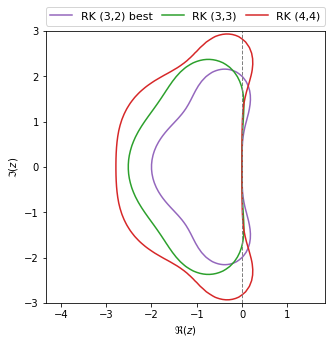
\includegraphics[width=0.3\textwidth]{\localPath/figures/rk_sd.png}
    \caption{The domain of stability for some classic explicit Runge--Kutta methods is shown. The nomenclature \textit{RK(s,p)} denotes a method with $s$ stages that is of order $p$. The Butcher tableaus of these methods are given in Appendix \ref{butcher}.
    }
	\label{fig:RK_sd2}
\end{figure}


\subsection{Exponential integrators}

We now apply commonly used exponential integrators to the test equation \eqref{ode_linear}. In this work we will consider the following methods: ExpRK22 (a classic two stage second order method), the method of Cox--Matthews \cite{cox}, the method of Hochbruck--Ostermann  \cite{hochbruck2005}, and the method of Krogstad \cite{krogstad2005}. We refer to \cite{ei} for more details and to Appendix \ref{butcher} for the Butcher tableaus of these methods. 

For the sake of brevity we will only detail the calculation for the ExpRK22 scheme. Applying this method to the test equation we obtain
\begin{eqnarray*}
k_1&=&e^{ia\Delta t}u^n + \Delta t\varphi_1(ia\Delta t)\lambda u^n\nonumber\\
u^{n+1}&=& e^{ia\Delta t}u^n + \Delta t \Big[ (\varphi_1(ia\Delta t)-\varphi_2(ia\Delta t))\lambda u^n + \varphi_2(ia\Delta t)\lambda k_1\Big], 
\end{eqnarray*}
where $\varphi_1(z)=(e^{z}-1)/z$ and $\varphi_2(z)=(e^{z}-1-z)/z^2$ are entire functions. This yields the stability function
\[ \phi(z) = e^{ia\Delta t} + \Big(\varphi_1(ia\Delta t)-\varphi_2(ia\Delta t)+e^{ia\Delta t}\varphi_2(ia\Delta t)\Big)z + \varphi_1(ia\Delta t)\varphi_2(ia\Delta t)z^2, \]
where, as before, we use $z=\lambda \Delta t$.

Our first observation is that, in contrast to Lawson methods, the behavior of this stability function can not be understood by the domain of stability of the underlying $RK(2, 2)$ method, \ie~the explicit method we obtain if we take $a \to 0$. In fact, as we vary $a$ the domain of stability changes drastically. The domain of stability for the four exponential integrators (ExpRK22, Cox--Matthews, Hochbruck--Ostermann, and Krogstad) is plotted in Figure~\ref{fig:expRK_sd} for $a\Delta t=1.1$ and $a\Delta t=3.4$. It is most striking that for large $\vert a\Delta t \vert$ the domain of stability does not contain a symmetric interval of the imaginary axis. It should be evident that this has the potential to causes severe stability issues.

\begin{figure}[h]
	\centering
	\begin{subfigure}[b]{0.3\textwidth}
		\centering 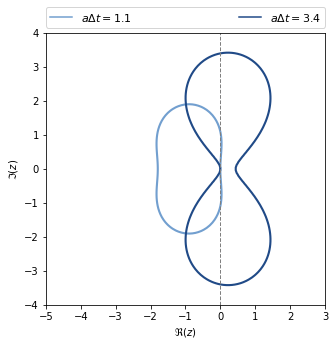
\includegraphics[width=\textwidth]{\localPath/figures/expRK22_sd.png}
	\end{subfigure}
	\begin{subfigure}[b]{0.3\textwidth}
		\centering 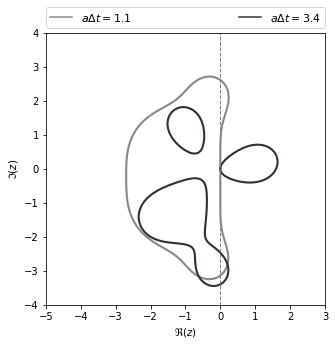
\includegraphics[width=\textwidth]{\localPath/figures/K_sd.png}
	\end{subfigure}

	\begin{subfigure}[b]{0.3\textwidth}
		\centering 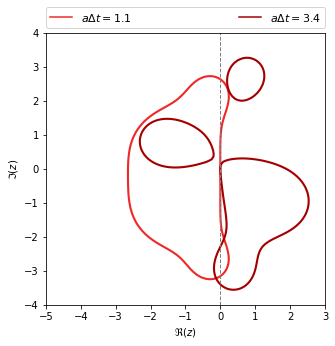
\includegraphics[width=\textwidth]{\localPath/figures/CM_sd.png}
	\end{subfigure}
		\begin{subfigure}[b]{0.3\textwidth}
		\centering 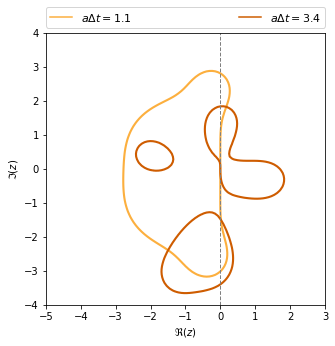
\includegraphics[width=\textwidth]{\localPath/figures/HO_sd.png}
	\end{subfigure}
    \caption{Stability domain of exponential integrators for two different values of $a\Delta t\in\{1.1, 3.4\}$.  From top left to bottom right: ExpRK22,  Krogstad, Cox--Matthews and Hochbruck--Ostermann.}  
	\label{fig:expRK_sd}
\end{figure}



%%%%%%%%%%%%%%%%%%%%%%%%%%%%%%%%%%
%%%%%%%%%%%%%%%%%%%%%%%%%%%%%%%%%%

\subsection{Phase space discretization}

We start from the two-dimensional linear transport equation
\begin{equation}
	\label{vp_linear}
    \partial_t f + d\partial_x f + b\partial_v f = 0, \;\; d, b\in\mathbb{R}, \;\; x\in [0, 2 \pi], \;\; v\in [-v_{\max},v_{\max}], 
\end{equation}
where $v_{\max}>0$  refers to the truncated velocity domain. 
The sought-after distribution function is $f(t,x,v)$ and we impose periodic boundary conditions in the $x$-direction. We assume that $d$ and $b$ are constants and thus the corresponding operators commute. This is an idealization of the Vlasov equation we will consider in the next section. In preparation for that example it is most useful to think that $d$ is large and thus would induce a stringent CFL condition if discretized by an explicit scheme.

We now have to discretize this equation both in the $x$ and the $v$ direction. In the spatial direction $x$, we will consider a spectral approximation. Performing a Fourier transformation of equation \eqref{vp_linear} yields
\begin{equation} 
\label{fourier_x_vlasov}
\partial_t \hat{f}_{k} +  i d k\hat{f}_{k} +b \partial_v \hat{f}_{k} = 0,
\end{equation} 
where $\hat{f}_k(t,v)$ denotes the Fourier transform of $f(t,x,v)$ with respect to $x$. The corresponding frequency is denoted by $k$. 

We now perform the discretization in the $v$ direction. The grid points are denoted by $v_j=-v_{\max}+j \Delta v$, with $\Delta v=2v_{\max}/N_v$, where $N_v$ is the number of points. We will consider two options here. Namely, either using a centered difference scheme or an upwind scheme.




\paragraph{Centered scheme in $v$.\\} The classic centered scheme is obtained by approximating the velocity derivative in equation \eqref{fourier_x_vlasov} by
$$
(\partial_v \hat{f}_{k})(v_j) \approx \frac{\hat{f}_{k, j+1}-\hat{f}_{k, j-1}}{2\Delta v},
$$ 
where $\hat{f}_{k,j}$ is an approximation of $\hat{f}_{k}(v_j)$.  Inserting this centered approximation 
in \eqref{fourier_x_vlasov} yields
\begin{equation} \label{eq:half-fourier}
\partial_t \hat{f}_{k,j} +  i d k\hat{f}_{k,j} +b \frac{\hat{f}_{k,j+1} -\hat{f}_{k,j-1} }{2\Delta v} = 0. \end{equation}
The system is already diagonal with respect to the index $k$. We now also diagonalize it with respect to the index $j$. To do that we express the function in terms of its Fourier modes with respect to $v$. That is,
\[ \hat{f}_{k,j} = \sum_m \bar{f}_{k, m}\exp\left(i \frac{2\pi m}{2v_{\max}}  v_j\right), \]
where $\bar{f}_{k,m}$ denotes the (double) Fourier transform of $f$ with frequency in space $k$ and frequency in velocity $m$. Inserting this into equation \eqref{eq:half-fourier} yields
\begin{equation}
\label{discrete_linear_transport}
	\partial_t \bar{f}_{k,m} + i dk\bar{f}_{k,m} +b \frac{i\sin(2\pi m \Delta v/(2v_{\max})) }{\Delta v} \bar{f}_{k,m}= 0.  
\end{equation}
We immediately see that this equation is precisely in the form of equation \eqref{ode_linear} as studied in the previous section. We also observe that $\lambda \in i\mathbb{R}$. That is, the eigenvalues for the centered difference approximation lie exclusively on the imaginary axis. One immediate consequence is that for Lawson methods the CFL condition is given by $b \Delta t < C \Delta v$, where $C$ is chosen such that $i [-C,C]$ lies in the domain of stability of the underlying Runge--Kutta method.



\paragraph{Linearized WENO approximation in $v$.\\} 

A common technique to discretize hyperbolic partial differential equations is to use the so-called weighted essentially non-oscillatory schemes (WENO) schemes. These are nonlinear schemes that limit oscillations in regions where sharp gradients occur, but still yield high order accuracy in smooth regions of the phase space. In the linear case WENO schemes reduce to upwind discretizations. Here, we will consider the LW5 scheme (the linearized version of the WENO5 scheme as considered in \cite{baldauf, lunet, motamed, wang}) that is given by (from now on we assume w.l.o.g.~that $b>0$)
\begin{align*}
(\partial_v \hat{f}_k)(v_j) &\approx \frac{1}{\Delta v}\Big(-\frac{1}{30} \hat{f}_{k,j-3} +\frac{1}{4} \hat{f}_{k,j-2} -\hat{f}_{k,j-1} + \frac{1}{3} \hat{f}_{k,j} +\frac{1}{2} \hat{f}_{k,j+1} - \frac{1}{20} \hat{f}_{k,j+2}\Big). 
\end{align*}
We now perform the same analysis as for the centered scheme (see \cite{baldauf, fov}). This yields
\begin{align}
  {\color{black} \left( \frac{2\pi }{2 v_{\max}}  i m \bar{f}_{k, m} \approx \right)}
   %(i m \bar{f}_{k, m} \approx ) \;\; 
   \mu_m \bar{f}_{k, m} &:= \frac{\bar{f}_{k,m}}{\Delta v}\Big(-\frac{1}{30} e^{-\frac{3i m\pi \Delta v}{v_{\max}}} +\frac{1}{4} e^{-\frac{2i m \pi \Delta v}{v_{\max}}} -e^{-\frac{i m \pi \Delta v}{v_{\max}}}  \nonumber\\
&\hspace{1cm}+ \frac{1}{3}  +\frac{1}{2} e^{\frac{i m \pi \Delta v}{v_{\max}}} - \frac{1}{20} e^{\frac{2i m \pi \Delta v}{v_{\max}}}\Big). 
\label{lw5symbol}
\end{align}
We then obtain the equation 
\begin{equation}
	\label{discrete_linear_transport_weno}
	\partial_t \bar{f}_{k,m} + i dk\bar{f}_{k,m} +b \mu_m \bar{f}_{k,m}= 0.
\end{equation}
Once again this is precisely the form of equation \eqref{ode_linear}, where $a=dk\in\mathbb{R}$ and $\lambda=b\mu_m \in\mathbb{C}$. The main difference to the centered difference scheme is that $\lambda$ is not necessarily on the imaginary axis. In fact, the eigenvalues aquire a negative real part which stabilizes the scheme and avoids spurious oscillations, but also adds unphysical dissipation to the numerical method.

{\color{black} 
\begin{remark}
Let us remark that performing a Fourier approximation in $v$ is also possible. Using the same notation as before, the counterpart of \eqref{discrete_linear_transport} and \eqref{discrete_linear_transport_weno} in that case is
$$
\partial_t \bar{f}_{k,m} + i dk\bar{f}_{k,m} +b i \frac{2\pi m}{2 v_{\max}} \bar{f}_{k,m}= 0.
$$
It is worth mentioning that this last equation can be obtained by considering the limit $\Delta v$ goes to zero in  \eqref{discrete_linear_transport} or \eqref{discrete_linear_transport_weno}. The stability condition can be computed as for the centered difference case, since the eigenvalues of the Fourier approximation also lies on the imaginary axis. The CFL condition is given by $b \pi  < C \Delta v$, where $C$ is chosen such that $i [-C,C]$ lies in the domain of stability of the underlying Runge--Kutta method. 


\end{remark}
}

\subsection{Computing the CFL condition}

Equipped with the knowledge of the domain of stability for the time discretization and the eigenvalues of the space discretization, we are now in a position to determine the CFL condition for the linear transport equation \eqref{vp_linear}. This task will be rather easy to accomplish for the Lawson schemes, where the stability does not depend on the advection speed for the transport in the $x$ direction. However, for exponential integrators even this linear analysis is rather complicated, as we will see.


\subsubsection{Centered scheme in $v$.}
In the case of centered approximation of the velocity derivative, the Fourier multiplier is a 
pure imaginary complex number (see equation \eqref{discrete_linear_transport}). We thus look for $y_{\max}\in \mathbb{R}_+$ such that the interval $i(-y_{\max},y_{\max}) \subset {\cal D}$, where ${\cal D}$ is the domain of stability for the chosen time integrator. 

\paragraph{Lawson integrators.\\} 
We simply look for the largest value $y_{\max}$ such that $i(-y_{\max}, y_{\max}) \subset \mathcal{D}$. The corresponding values for a number of schemes are listed in Table \ref{tab:ymax_Lawson}. These values have to be understood in the 
following way: they induce the CFL condition $b \Delta t\leq y_{\max}\Delta v$ for the discretized equation \eqref{discrete_linear_transport}, where $\Delta t$ denotes the time step size and $\Delta v$ is the velocity mesh size. 



\begin{table}[h]
	\centering
	\begin{tabular}{|c|c|c|c|}
		\hline
		Methods & Lawson($RK(3,2) \; best$) & Lawson($RK(3,3)$) & Lawson($RK(4,4)$) \\
		\hline
		$y_{\max}$ & $2$ & $\sqrt{3}$ & $2\sqrt{2}$\\
		\hline  
	\end{tabular}
	\caption{CFL number for some Lawson schemes applied to \eqref{discrete_linear_transport}. }
	\label{tab:ymax_Lawson}
\end{table}


\paragraph{Exponential integrators. \\}

For the exponential integrators the domain of stability is very sensitive to the value of $(a\Delta t)$. To get an idea of what we can expect, we consider the quantity $y_{\max} = \min_{(a\Delta t)\in\mathbb{R}} \; y^{exp}_{\max}(a \Delta t)$. As before, $y^{exp}_{\max}(a\Delta t)$ is the largest value such that $i(-y^{exp}_{\max}(a\Delta t), y^{exp}_{\max}(a\Delta t))\subset {\cal D}$, where ${\cal D}$ is the domain of stability for the chosen exponential time integrator for a given $(a\Delta t)$. 
Even for relatively simple numerical methods it is not possible to compute this quantity analytically. Thus, we resort to numerical approximations. Unfortunately, it turns out that for most exponential integrators this value is zero. This can be appreciated by considering Figure \ref{fig:expRK_sd} once more. Clearly, there are values of $(a \Delta t)$ such that no relevant part of the imaginary axis (or only half the imaginary axis) is part of the domain of stability.
Thus, most exponential integrators are unstable in the von Neumann sense. However, this is not what we observe in practice. In fact, already the results presented in \cite{cep} indicate that we can successfully run numerical simulations using, for example, the Cox--Matthews scheme. There are two major points to consider here
\begin{itemize}
    \item The $y_{\max}$ obtained is a worst case estimate. In fact, we know that for $\Delta t \to 0$ we regain the stability of the underlying Runge--Kutta method. Thus, for small $(a \Delta t)$ the methods is expected to work well.
    \item As is usually done we have mandated that $\vert \phi(z) \vert \leq 1$. However, strictly speaking this is not necessary for practical simulation. If we assume that $\vert \phi(z) \vert \leq 1+\varepsilon$ and we take $n$ steps the amplification of the error is given by $(1+\varepsilon)^n$. In the limit $n \to +\infty$ this quantity diverges. However, since we usually do not take infinitely small time steps we still can hope to obtain a relatively accurate approximation, especially if $\varepsilon$ is small. \textcolor{black}{In particular, if $\varepsilon = C \Delta t = C t_{final}/n$ (where $t_{final}$ denotes the final time and $n$ the number of iterations) we have $(1+\varepsilon)^n = (1+\tfrac{C t_{final}}{n} )^n \leq \exp(C t_{final})$ and thus the scheme is stable, while the error constant is increased by $\exp(C t_{final})$.}
\end{itemize}


To investigate this further, we propose to relax the stability condition by introducing a threshold $\varepsilon>0$ 
in the definition of the stability domain
\begin{equation}
\label{d_eps}
	\mathcal{D}_\varepsilon = \{ z\in\mathbb{C} : |\phi(z)| \leq 1+\varepsilon \}. 
\end{equation}

In Figure~\ref{ymax_example}, we plot the domain of stability for the Cox--Matthews method and $a\Delta t = 3.4$ for $\varepsilon=0$ and $\varepsilon=10^{-2}$. One can observe that in the latter case a non-zero $y_{\max}^{exp}(3.4)$ is obtained. We also call attention to the fact that the part of the imaginary axis included in this relaxed stability domain is not symmetric. 

\begin{figure}[h]
  \centering
  \begin{subfigure}[b]{0.33\textwidth}
        \centering 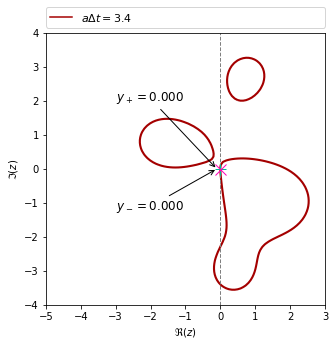
\includegraphics[width=\textwidth]{\localPath/figures/CM_sd_ymax_e0p00.png}
  \end{subfigure}
  \begin{subfigure}[b]{0.33\textwidth}
        \centering 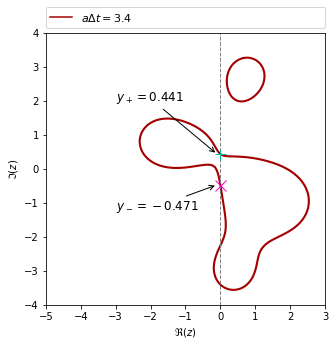
\includegraphics[width=\textwidth]{\localPath/figures/CM_sd_ymax_e0p01.png}
  \end{subfigure}
  \caption{Example of variation of $y_+$ and $y_-$ when we relax the stability condition for the Cox--Matthews scheme. We represent $\mathcal{D}_{0}$ on the left, and $\mathcal{D}_{10^{-2}}$ on the right with the values $y_+$ and $y_-$  such that 
  $i(y_-, y_+)\subset \mathcal{D}_{\varepsilon}$.}
  \label{ymax_example}
\end{figure}

In Figure \ref{ymax_expRK22}, we plot the dependence of $y^{exp}_{\max}$ as a function of $(a\Delta t)$ for $\varepsilon=10^{-2}$ and the ExpRK22 method. Let us recall that for $\varepsilon=0$, the method gives $y_{\max}=0$. One can observe that the  domain of stability 
${\cal D}_\varepsilon$  of this method is still symmetric with respect to the real axis. In addition, the method becomes more stable as $|a\Delta t|$ increases. Thus, the behavior of the method is completely different from the configuration with $\varepsilon=0$.

\begin{figure}[h]
	\centering
	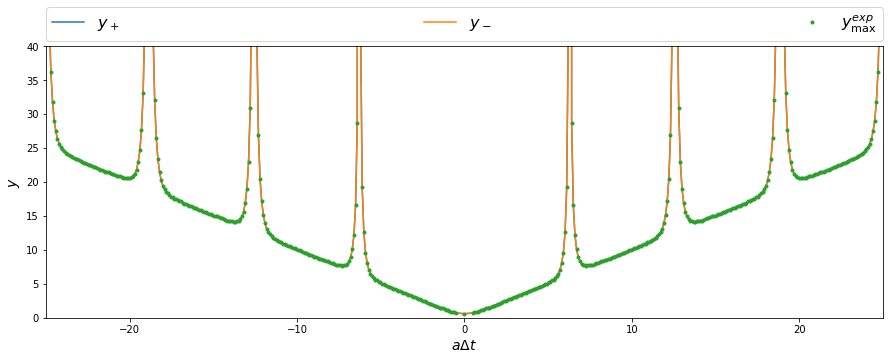
\includegraphics[scale=0.3]{\localPath/figures/ymax_expRK22_0p01}
    \caption{$y^{exp}_{\max}$, $|y_+|$ and $|y_-|$ as a function of $a \Delta t$ for the ExpRK22 method with $\varepsilon=10^{-2}$. } 
	\label{ymax_expRK22}
\end{figure}

In Figure \ref{ymax_HO}, we plot $y^{exp}_{\max}$ as a function of $(a\Delta t)$ for the Hochbruck--Ostermann method (once again for 
$\varepsilon=10^{-2}$). This schemes also gives $y_{\max}=0$ for $\varepsilon=0$. In this case the domain of stability is not symmetric 
and the stability depends quite erratically on the value of $(a \Delta t)$.
\begin{figure}[h]
	\centering
	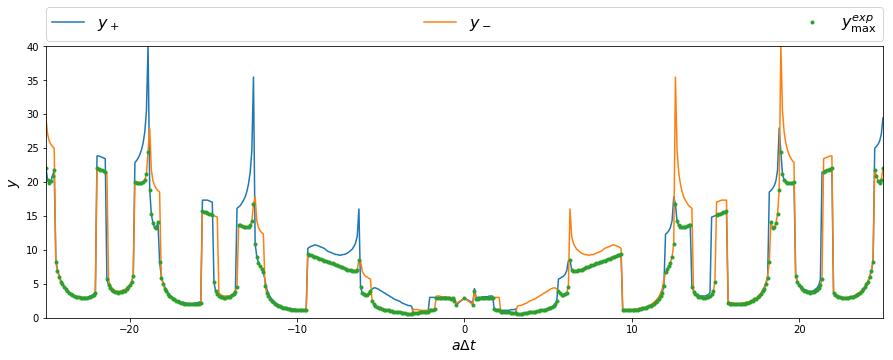
\includegraphics[scale=0.3]{\localPath/figures/ymax_HO_0p01}
	\caption{$y^{exp}_{\max}$, $|y_+|$ and $|y_-|$  as a function of $a\Delta t$ for the Hochbruck--Ostermann method with $\varepsilon=10^{-2}$.} 
	\label{ymax_HO}
\end{figure}
In Table \ref{tab:ymax_expo} we have summarized the values of $y_{\max}$ for the four exponential integrators considered in this paper.


\begin{table}
	\centering
	\begin{tabular}{|c|c|c|c|c|}
		\hline
		Methods                                & ExpRK22 & Krogstad & Cox--Matthews & Hochbruck--Ostermann      \\
		\hline
		$y^{exp}_{\max} (\varepsilon=10^{-3})$ & $0.300$ & $0.100$  & $0.150$      & $0.250$ \\
		\hline
		$y^{exp}_{\max} (\varepsilon=10^{-2})$ & $0.551$ & $0.200$  & $0.450$      & $0.501$ \\
		\hline  
		$y^{exp}_{\max} (\varepsilon=10^{-1})$ & $1.001$ & $0.601$  & $1.351$      & $1.702$ \\
		\hline  
	\end{tabular}
	\caption{CFL number, assuming the relaxed stability constraint, for some exponential integrators applied to \eqref{discrete_linear_transport}.}
	\label{tab:ymax_expo}
\end{table}

{\color{red}
Finally, we give an illustration of the above comments by running \eqref{vp_linear} ($d=b=1$ and $v_{\max}=3$) 
with a discontinuous initial data to study the impact of high-frequency on the stability of exponential schemes coupled 
with a centered scheme in $v$. 
The initial condition is 
$$
f_0(x, v) = 1 \mbox{ if } \sqrt{(x-\pi)^2+v^2} \leq 1, \mbox{ and } 0  \mbox{ elsewhere}. 
$$
From the stability analysis we know that for each $k$ it holds that $\bar{f}^{n+1}_{k,m} = \phi(z)\bar{f}^{n}_{k,m}$,
where $\phi$ is the stability function. 
Our study enables us to estimate the amplification factor $|\phi(z)|$ by $(1+\varepsilon)$ (uniformly with respect to $k$)  
so that $|\bar{f}^{n+1}_{k,m}|^2 \leq  (1+\varepsilon)^2 |\bar{f}^{n}_{k,m}|^2$. Hence, for a given $\varepsilon$, 
we consider a time step according to Table \ref{tab:ymax_expo} and run 
two exponential schemes, namely Hochbruck-Ostermann and Cox-Matthews,   
for $100$ timesteps. After each time step
we compute $\| f^n\|^2_{\ell^2} / \| f^0\|^2_{\ell^2}$. 
The results can be found in Figure \ref{instab}.   
\begin{figure}
\centering
\begin{tabular}{cc}
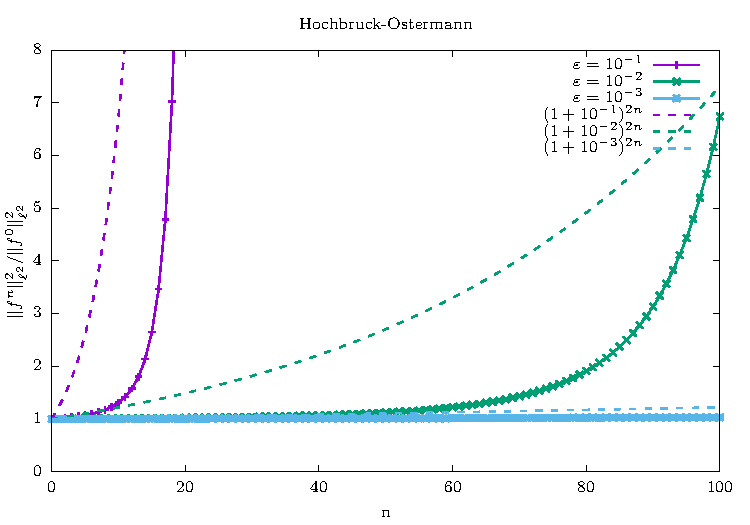
\includegraphics[scale=0.5]{\localPath/figures/error_growup_HO.pdf} & 
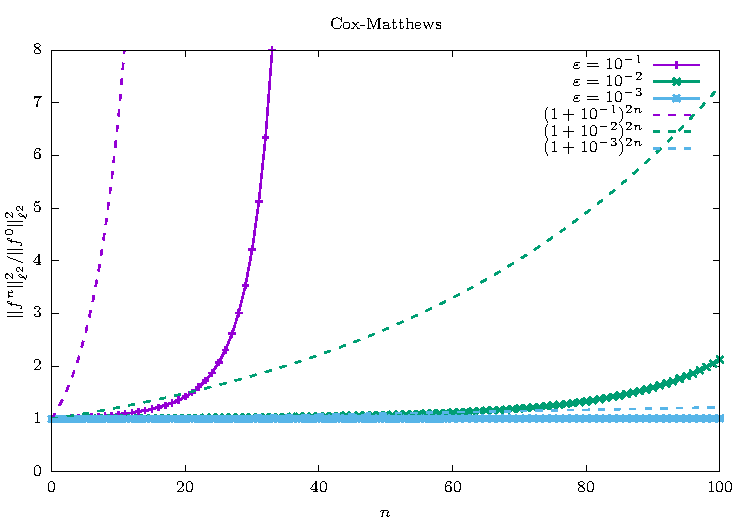
\includegraphics[scale=0.5]{\localPath/figures/error_growup_CM.pdf} 
\end{tabular}
\caption{Evolution of $\| f^n\|^2_{\ell^2} / \| f^0\|^2_{\ell^2}$ and of $(1+\varepsilon)^{2n}$ as a function of $n$ for different values of 
$\varepsilon$. Left: Hochbruck-Ostermann scheme. Right: Cox-Matthews scheme. }
\label{instab}
\end{figure}
First, we have a numerical confirmation that $(1+\varepsilon)$ is an estimate of the amplification factor 
(the ratio $\| f^n\|^2_{\ell^2} / \| f^0\|^2_{\ell^2}$  always lies under the curve $n\mapsto (1+\varepsilon)^{2n}$).  
Second, since the number of time steps is fixed, for $\varepsilon=0.1$ the simulation becomes unstable for $n\geq 20$. 
As soon as $\varepsilon$ is small enough, the simulation is stable. 
%As mentioned above, if $\varepsilon$ as $\varepsilon =C \Delta t = Ct_{final}/n$  
%(with $\Delta t=y_{\max} \Delta v$, $y_{\max}$ being given by Table \ref{tab:ymax_expo} and $\Delta v=6/81$), 
%the scheme is  stable and considering a final time $t_{final} = n\Delta t$, the linear analysis leads to 
%\begin{eqnarray*}
%\|{f}^{n}\|_{\ell^2} &=& \|\bar{f}^{n}\|_{\ell^2} \leq  (1+\varepsilon)^n \|\bar{f}^{0}\|_{\ell^2} =  (1+C\Delta t)^{t_{final}/\Delta t} \|\bar{f}^{0}\|_{\ell^2} \nonumber\\
%&\leq & \exp(Ct_{final}) \|\bar{f}^{0}\|_{\ell^2} = \exp(Ct_{final}) \|{f}^{0}\|_{\ell^2}, 
%\end{eqnarray*}
%which gives some practical informations on the stability of the methods since $C$ and $t_{final}$ are known a priori. 
}

\subsubsection{Linearized WENO5 (LW5) scheme. }

In the case of a WENO5 approximation of the velocity derivative, we can not 
easily find a Fourier multiplier because of its nonlinearity. 
Recent studies about stability of WENO5 \cite{wang, motamed, lunet} considered 
the linearized version of WENO schemes by freezing the nonlinear weights, 
so that WENO5 reduces to a high order (linear) upwind scheme called LW5. For this LW5 scheme we can
compute the eigenvalues, see equation \eqref{lw5symbol}, 
and different time stepping schemes can be studied to determine the stability limit. 
We consider only Lawson methods here since we found 
that the exponential schemes we considered (\ie{}~ExpRK22, Krogstad, Cox--Matthews, Hochbruck--Ostermann) 
lead to unstable results when they are combined with LW5 (even in the weak sense considered in the previous section).

The goal  is then to determine the largest non-negative real number $\sigma>0$ such that the 
eigenvalues of the upwind scheme LW5 scaled by $\sigma$ are contained in the domain of stability for the 
time integrator. Since the eigenvalues of LW5 are not as simple as in the case of the centered scheme, we determine $\sigma$ numerically. The main idea of the algorithm to obtain an estimation of $\sigma$ is:
\begin{enumerate}
    \item The argument $\varphi$ of the eigenvalues $\mu_m$  (normalized by $\Delta v$) given by \eqref{lw5symbol} are discretized using a fine angular grid $\{ \varphi_k\} \subset [-\pi/2, \pi/2]$, since the real part of $\mu_{m}$ is negative due to its diffusive character.
  \item A discretized version of the boundary of the stability domain of the underlying Runge--Kutta method is computed.
  \item For each discretized eigenvalue, we look for the closest boundary point of the Runge--Kutta stability domain. 
  This enables us to compute the associated stretching factor $\sigma(\varphi_k)$.
  \item Taking the minimum over all the discretized eigenvalues yields $\sigma:=\min_{k} \sigma(\varphi_k)$. 
\end{enumerate}




In Figure \ref{cfl_rk44_lw5} (left), we plot the dependence of $\sigma$ with respect to the angle $\varphi\in [-\pi/2, \pi/2]$ 
for Lawson($RK(4, 4)$) coupled with LW5. We also plot (Figure \ref{cfl_rk44_lw5} (right)) the stability domain of Lawson($RK(4, 4)$), 
the eigenvalues for LW5 (normalized by $\Delta v$) and the eigenvalues for LW5 scaled by $\sigma$. 
The CFL number for some Lawson schemes is shown in Table \ref{tab:ymax_weno_Lawson}. It is interesting to note that the time step size is  reduced compared to the centered scheme.
\begin{table}[h]
	\centering
	\begin{tabular}{|c|c|c|c|}
		\hline
		Methods & Lawson($RK(3,2) \; best$) & Lawson($RK(3,3)$) & Lawson($RK(4,4)$) \\
		\hline
		$\sigma $ & $1.344$ & $1.433$   & $1.73$   \\
		\hline  
	\end{tabular}
	\caption{CFL number for some Lawson schemes applied to \eqref{discrete_linear_transport_weno}. }
	\label{tab:ymax_weno_Lawson}
\end{table}

\begin{figure}[h]
  \centering
  \begin{subfigure}[b]{0.4\textwidth}
        \centering 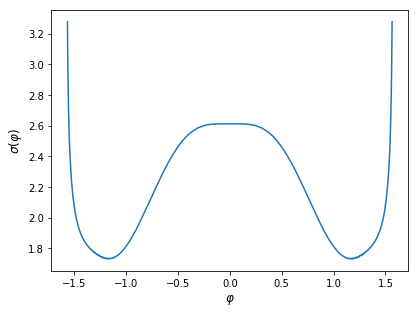
\includegraphics[width=\textwidth]{\localPath/figures/cfl_rk44_weno_phi.png}
  \end{subfigure}
  \begin{subfigure}[b]{0.3\textwidth}
        \centering 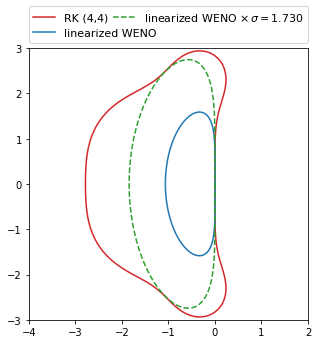
\includegraphics[width=\textwidth]{\localPath/figures/cfl_rk44_weno.png}
  \end{subfigure}
  \caption{Left: $\sigma$ as a function of the angle $\varphi$. Right: stability domain of Lawson($RK(4,4)$) (red), 
  eigenvalues for LW5 normalized by $\Delta v$ (blue) and eigenvalues for LW5 normalized by $\Delta v$ 
  stretched with factor $\sigma=1.73$ (dashed green). } 
  \label{cfl_rk44_lw5}
\end{figure}

%%%%%%%%%%%%%%%%%%%%%%%%%%%%%%%
\section{Numerical simulation: Vlasov-Poisson equations \label{sec:vp}}

In this section we apply Lawson methods and exponential integrators to the Vlasov-Poisson system. We will see that the linear theory developed in the last section gives a good indication of the stability even for this nonlinear problem. We consider a distribution function $f(t, x, v)$ depending on time $t\geq 0$, space $x$, with periodic boundary conditions, and velocity $v$, which satisfies the Vlasov equation 
\begin{equation}
	\label{vlasov}
    \partial_t f(t, x, v) + v\partial_x f(t, x, v) + E(f)(t, x)\partial_v f(t, x, v) = 0   
\end{equation}
coupled to a Poisson problem for the electric field $E(f)(t, x)$ 
\begin{equation}
    \partial_x  E(f)(t, x)= \int_{\mathbb{R}} f(t, x, v) \,dv -1. 
\end{equation}
We employ a Fourier approximation in space. In velocity we either use a centered discretization
$$
\partial_t \hat{f}_{k,j} + v_j i k \hat{f}_{k,j} + \Widehat{\Big(E_{\cdot} \frac{f_{\cdot,j+1}  -f_{\cdot,j-1}}{2\Delta v}\Big)}_k = 0
$$  
or the WENO5 discretization
\begin{equation}
    \displaystyle\partial_t \hat{f}_{k,j} + v_j ik \hat{f}_{k,j} + \Widehat{\Big(E^+_{\cdot} \frac{f^+_{\cdot,j+1/2} - f^+_{\cdot,j-1/2}}{\Delta v} \Big)}_k 
+ \Widehat{\Big(E^-_{\cdot} \frac{f^-_{\cdot,j+1/2} - f^-_{\cdot,j-1/2}}{\Delta v} \Big)}_k = 0, 
\label{vp_weno}
\end{equation} 
where $E^+=\max(E, 0)$, $E^-=\min(E, 0)$ and $f^\pm_{j+1/2}$ denote the numerical fluxes (see Appendix \ref{app_weno} for more details). Both of these phase space discretizations can be easily cast in the following form
\[ \partial_t \hat{f}_{k,j} = - v_j i k \hat{f}_{k,j} + F(f)_{k,j}, \]
for an appropriately defined $F$. We can now apply an exponential integrator or a Lawson scheme. To illustrate this let us consider the exponential Euler method. This gives
\[ \hat{f}^{n+1}_{k,j} = \exp(-\Delta t v_j i k) \hat{f}^n_{k,j} + \Delta t \varphi_1(-\Delta t v_j i k) F(f^n)_{k,j}. \]
Since in Fourier space the exponential and $\varphi_1$ functions have only scalar arguments, their computation is easy and efficient (\ie~no matrix functions have to be computed). Due to the nonlinearity, it is favorable to compute $E \partial_v f$ in real space. This is done efficiently by using the fast Fourier transform. Generalizing this scheme to multiple dimensions in both space and velocity is straightforward.


To apply our theory from the linear analysis to the nonlinear Vlasov-Poisson case, we need a way to compute the CFL condition. Note that the coefficient of the $v$ advection depends on $E$ and thus implicitly on time. We choose the time step for the centered scheme as follows
\begin{equation}
\label{cfl_vlasov_lc}
\Delta t_n = \frac{y_{\max} \Delta v}{\| E^n \|_{L^\infty}}, 
\end{equation}
whereas for the WENO5 scheme we use the CFL condition computed from its linearized version (LW5)
\begin{equation}
\label{cfl_vlasov_lw}
\Delta t_n = \frac{\sigma \Delta v}{\| E^n \|_{L^\infty}}.
\end{equation}
The value $\| E^n \|_{L^\infty}$ is just the maximal value of the electric field at time $t_n$. The values for  $y_{\max}$ and $\sigma$ are given in Tables \ref{tab:ymax_Lawson}, \ref{tab:ymax_expo}, and \ref{tab:ymax_weno_Lawson} according to the chosen time integrator. 


\subsection{Landau damping test.} 

We present numerical results for the standard Landau damping test case. The initial condition is given by
$$
f_0(x, v) = \frac{1}{\sqrt{2\pi}} e^{-\frac{v^2}{2}} (1+0.001 \cos(0.5 x)), \;\; x\in [0, 4\pi], v\in \mathbb{R}. 
$$
The numerical parameters are chosen as follows: the number of points in space is $N_x=81$ whereas the velocity domain 
is truncated to $[-v_{\max}, v_{\max}]$ with $v_{\max}=8$ and is discretized with $N_v=128$ grid points.

Let us remark that for the Landau damping test, the conditions \eqref{cfl_vlasov_lc} and 
\eqref{cfl_vlasov_lw} allow us to take very large time steps, since $\| E^n \|_{L^\infty} \leq \| E^0 \|_{L^\infty} = 2\cdot 10^{-3}$. Then, 
we get $\Delta t = C \Delta v \; 0.5\cdot 10^3 =  62.5 C$, where $C$ can be either $y_{\max}$ or $\sigma$ depending on the chosen time integrator. This means that in practice we can choose the time step $\Delta t$ independently from the mesh. This is clearly a desirable desirable feature of the time integrator.

In Figure \ref{ld}, the time history of the electric energy $\|E^n\|_{L^2}$ (in semi-log scale) 
{\color{black} using Lawson($RK(4, 4)$)-WENO5 (with two different time steps $\Delta t=1/8$ and $\Delta t=1$), 
and using Hochbruck--Ostermann-CD2 (with $\Delta t=1$).   
One can observe that the expected damping rate  
($\gamma=-0.153$) is recovered for the three schemes. Although, the accuracy deteriorates for $\Delta t=1$ Lawson($RK(4, 4)$)-WENO5, 
the Hochbruck--Ostermann-CD2 scheme gives very good results even with $\Delta t=1$. We note that all the numerical schemes are clearly stable. }
\begin{figure}[h]
	\centering
%	% GNUPLOT: LaTeX picture with Postscript
\begingroup
  \makeatletter
  \providecommand\color[2][]{%
    \GenericError{(gnuplot) \space\space\space\@spaces}{%
      Package color not loaded in conjunction with
      terminal option `colourtext'%
    }{See the gnuplot documentation for explanation.%
    }{Either use 'blacktext' in gnuplot or load the package
      color.sty in LaTeX.}%
    \renewcommand\color[2][]{}%
  }%
  \providecommand\includegraphics[2][]{%
    \GenericError{(gnuplot) \space\space\space\@spaces}{%
      Package graphicx or graphics not loaded%
    }{See the gnuplot documentation for explanation.%
    }{The gnuplot epslatex terminal needs graphicx.sty or graphics.sty.}%
    \renewcommand\includegraphics[2][]{}%
  }%
  \providecommand\rotatebox[2]{#2}%
  \@ifundefined{ifGPcolor}{%
    \newif\ifGPcolor
    \GPcolorfalse
  }{}%
  \@ifundefined{ifGPblacktext}{%
    \newif\ifGPblacktext
    \GPblacktexttrue
  }{}%
  % define a \g@addto@macro without @ in the name:
  \let\gplgaddtomacro\g@addto@macro
  % define empty templates for all commands taking text:
  \gdef\gplbacktext{}%
  \gdef\gplfronttext{}%
  \makeatother
  \ifGPblacktext
    % no textcolor at all
    \def\colorrgb#1{}%
    \def\colorgray#1{}%
  \else
    % gray or color?
    \ifGPcolor
      \def\colorrgb#1{\color[rgb]{#1}}%
      \def\colorgray#1{\color[gray]{#1}}%
      \expandafter\def\csname LTw\endcsname{\color{white}}%
      \expandafter\def\csname LTb\endcsname{\color{black}}%
      \expandafter\def\csname LTa\endcsname{\color{black}}%
      \expandafter\def\csname LT0\endcsname{\color[rgb]{1,0,0}}%
      \expandafter\def\csname LT1\endcsname{\color[rgb]{0,1,0}}%
      \expandafter\def\csname LT2\endcsname{\color[rgb]{0,0,1}}%
      \expandafter\def\csname LT3\endcsname{\color[rgb]{1,0,1}}%
      \expandafter\def\csname LT4\endcsname{\color[rgb]{0,1,1}}%
      \expandafter\def\csname LT5\endcsname{\color[rgb]{1,1,0}}%
      \expandafter\def\csname LT6\endcsname{\color[rgb]{0,0,0}}%
      \expandafter\def\csname LT7\endcsname{\color[rgb]{1,0.3,0}}%
      \expandafter\def\csname LT8\endcsname{\color[rgb]{0.5,0.5,0.5}}%
    \else
      % gray
      \def\colorrgb#1{\color{black}}%
      \def\colorgray#1{\color[gray]{#1}}%
      \expandafter\def\csname LTw\endcsname{\color{white}}%
      \expandafter\def\csname LTb\endcsname{\color{black}}%
      \expandafter\def\csname LTa\endcsname{\color{black}}%
      \expandafter\def\csname LT0\endcsname{\color{black}}%
      \expandafter\def\csname LT1\endcsname{\color{black}}%
      \expandafter\def\csname LT2\endcsname{\color{black}}%
      \expandafter\def\csname LT3\endcsname{\color{black}}%
      \expandafter\def\csname LT4\endcsname{\color{black}}%
      \expandafter\def\csname LT5\endcsname{\color{black}}%
      \expandafter\def\csname LT6\endcsname{\color{black}}%
      \expandafter\def\csname LT7\endcsname{\color{black}}%
      \expandafter\def\csname LT8\endcsname{\color{black}}%
    \fi
  \fi
    \setlength{\unitlength}{0.0500bp}%
    \ifx\gptboxheight\undefined%
      \newlength{\gptboxheight}%
      \newlength{\gptboxwidth}%
      \newsavebox{\gptboxtext}%
    \fi%
    \setlength{\fboxrule}{0.5pt}%
    \setlength{\fboxsep}{1pt}%
\begin{picture}(7200.00,5040.00)%
    \gplgaddtomacro\gplbacktext{%
      \csname LTb\endcsname%%
      \put(814,704){\makebox(0,0)[r]{\strut{}$-18$}}%
      \put(814,1292){\makebox(0,0)[r]{\strut{}$-16$}}%
      \put(814,1880){\makebox(0,0)[r]{\strut{}$-14$}}%
      \put(814,2468){\makebox(0,0)[r]{\strut{}$-12$}}%
      \put(814,3055){\makebox(0,0)[r]{\strut{}$-10$}}%
      \put(814,3643){\makebox(0,0)[r]{\strut{}$-8$}}%
      \put(814,4231){\makebox(0,0)[r]{\strut{}$-6$}}%
      \put(814,4819){\makebox(0,0)[r]{\strut{}$-4$}}%
      \put(946,484){\makebox(0,0){\strut{}$0$}}%
      \put(1678,484){\makebox(0,0){\strut{}$5$}}%
      \put(2410,484){\makebox(0,0){\strut{}$10$}}%
      \put(3142,484){\makebox(0,0){\strut{}$15$}}%
      \put(3875,484){\makebox(0,0){\strut{}$20$}}%
      \put(4607,484){\makebox(0,0){\strut{}$25$}}%
      \put(5339,484){\makebox(0,0){\strut{}$30$}}%
      \put(6071,484){\makebox(0,0){\strut{}$35$}}%
      \put(6803,484){\makebox(0,0){\strut{}$40$}}%
    }%
    \gplgaddtomacro\gplfronttext{%
      \csname LTb\endcsname%%
      \put(308,2761){\rotatebox{-270}{\makebox(0,0){\strut{}$||E(t)||_{L^2}$}}}%
      \put(3874,154){\makebox(0,0){\strut{}$t$}}%
      \csname LTb\endcsname%%
      \put(5816,4646){\makebox(0,0)[r]{\strut{}Lawson$(RK(4,4))$ - WENO5 $\Delta t = 1/8$}}%
      \csname LTb\endcsname%%
      \put(5816,4426){\makebox(0,0)[r]{\strut{}Lawson$(RK(4,4))$ - WENO5 $\Delta t = 1$}}%
      \csname LTb\endcsname%%
      \put(5816,4206){\makebox(0,0)[r]{\strut{}slope $-0.153$}}%
    }%
    \gplbacktext
    \put(0,0){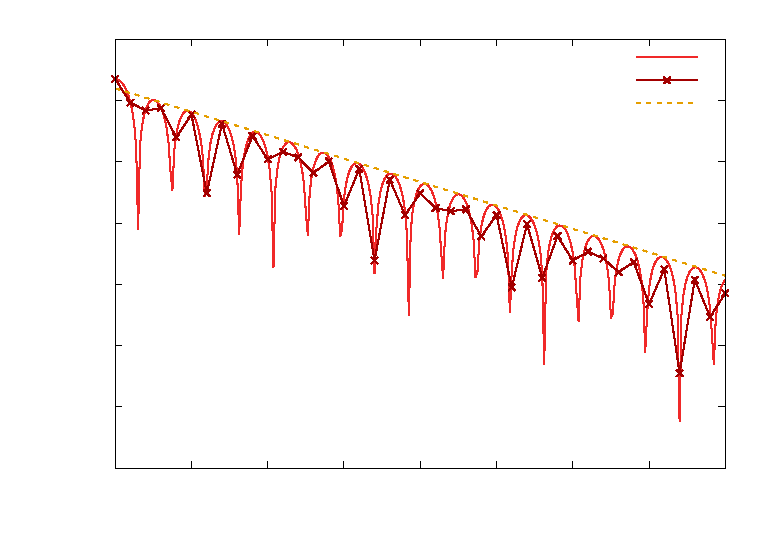
\includegraphics{img/Emax}}%
    \gplfronttext
  \end{picture}%
\endgroup

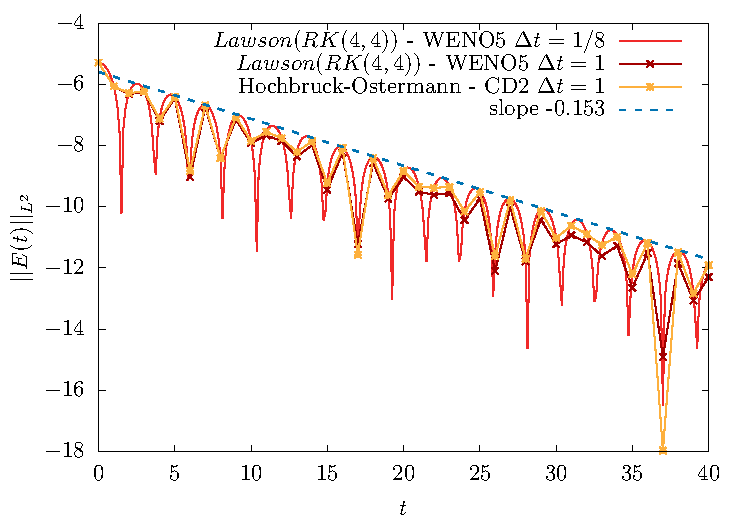
\includegraphics[width=\textwidth]{\localPath/figures/linear_landau.pdf}
	\caption{Landau damping test: time history of $\|E(t)\|_{L^2}$ (semi-log scale) obtained with Lawson($RK(4, 4)$) and WENO5 
	(with $\Delta t=1/8$ and $\Delta t=1$) {\color{black} and with Hochbruck-Ostermann and CD2 (with $\Delta t=1$)}.}
	\label{ld}
\end{figure}



\subsection{Bump on tail test.}

Next, we consider the bump on tail test for which the initial condition is 
$$
f_0(x, v) = \left[\frac{0.9}{\sqrt{2\pi}} e^{-\frac{v^2}{2}} + \frac{0.2}{\sqrt{2\pi}} e^{-2(v-4.5)^2} \right](1+0.04 \cos(0.3 x)), \;\; x\in [0, 20\pi], v\in \mathbb{R}. 
$$
The numerical parameters are chosen as follows: the number of points in space is $N_x=135$ 
whereas the velocity domain $[-v_{\max}, v_{\max}]$ (with $v_{\max}=8$) is discretized with $N_v=256$ grid points. 
Concerning the time step, 
as in the Landau damping example, the conditions \eqref{cfl_vlasov_lc} and \eqref{cfl_vlasov_lw} turn out to be very light for Lawson schemes. 
Indeed, we found $\max_n \| E^n \|_{L^\infty} \approx 0.6$ 
so that, with the considered velocity grid, the time step has to be smaller than $0.14$ 
in the worst case (Lawson($RK(3, 2) \; best)$ combined with WENO5). 
To capture correctly the phenomena involved in the bump on tail test, we take the following time step size
\begin{equation}
\label{dtbot}
\Delta t_n = \min \Big( 0.1,  \frac{C \Delta v}{\|E^n\|_{L^\infty}} \Big), 
\end{equation}
with $C=y_{\max}$ or $\sigma$ depending on the chosen scheme. Thus, also in this configuration we are mostly limited by the accuracy 
and not by the stability constraint.

{\color{black} In Figure \ref{space}, the full distribution function $f$ is plotted at time $t=40$ ($\Delta t=0.05$) for different schemes (exponential or Lawson in time 
and WENO or centered differences in velocity). One can observe spurious oscillations when the centered differences scheme case is used (second and third rows) whereas the slope 
limiters of WENO5 (first line) are able to control this phenomena so that extremas are well preserved. This is consistent with what has been observed in the literature.}

%In Figure \ref{space}, the full distribution function $f$ is plotted at time $t=40$ for 
%Lawson($RK(4, 4)$) coupled with the WENO5 scheme, Lawson($RK(4, 4)$) coupled with the centered scheme 
%and Hochbruck--Ostermann coupled with the centered scheme. In these figures, we look at the impact of the velocity 
%approximation.  One can observe spurious oscillations in the centered scheme case (middle figure) whereas the slope 
%limiters of WENO5 are able to control this phenomena so that extremas are well preserved. This is consistent with what has been observed in the literature.

\begin{figure}
\begin{tabular}{ccc}
    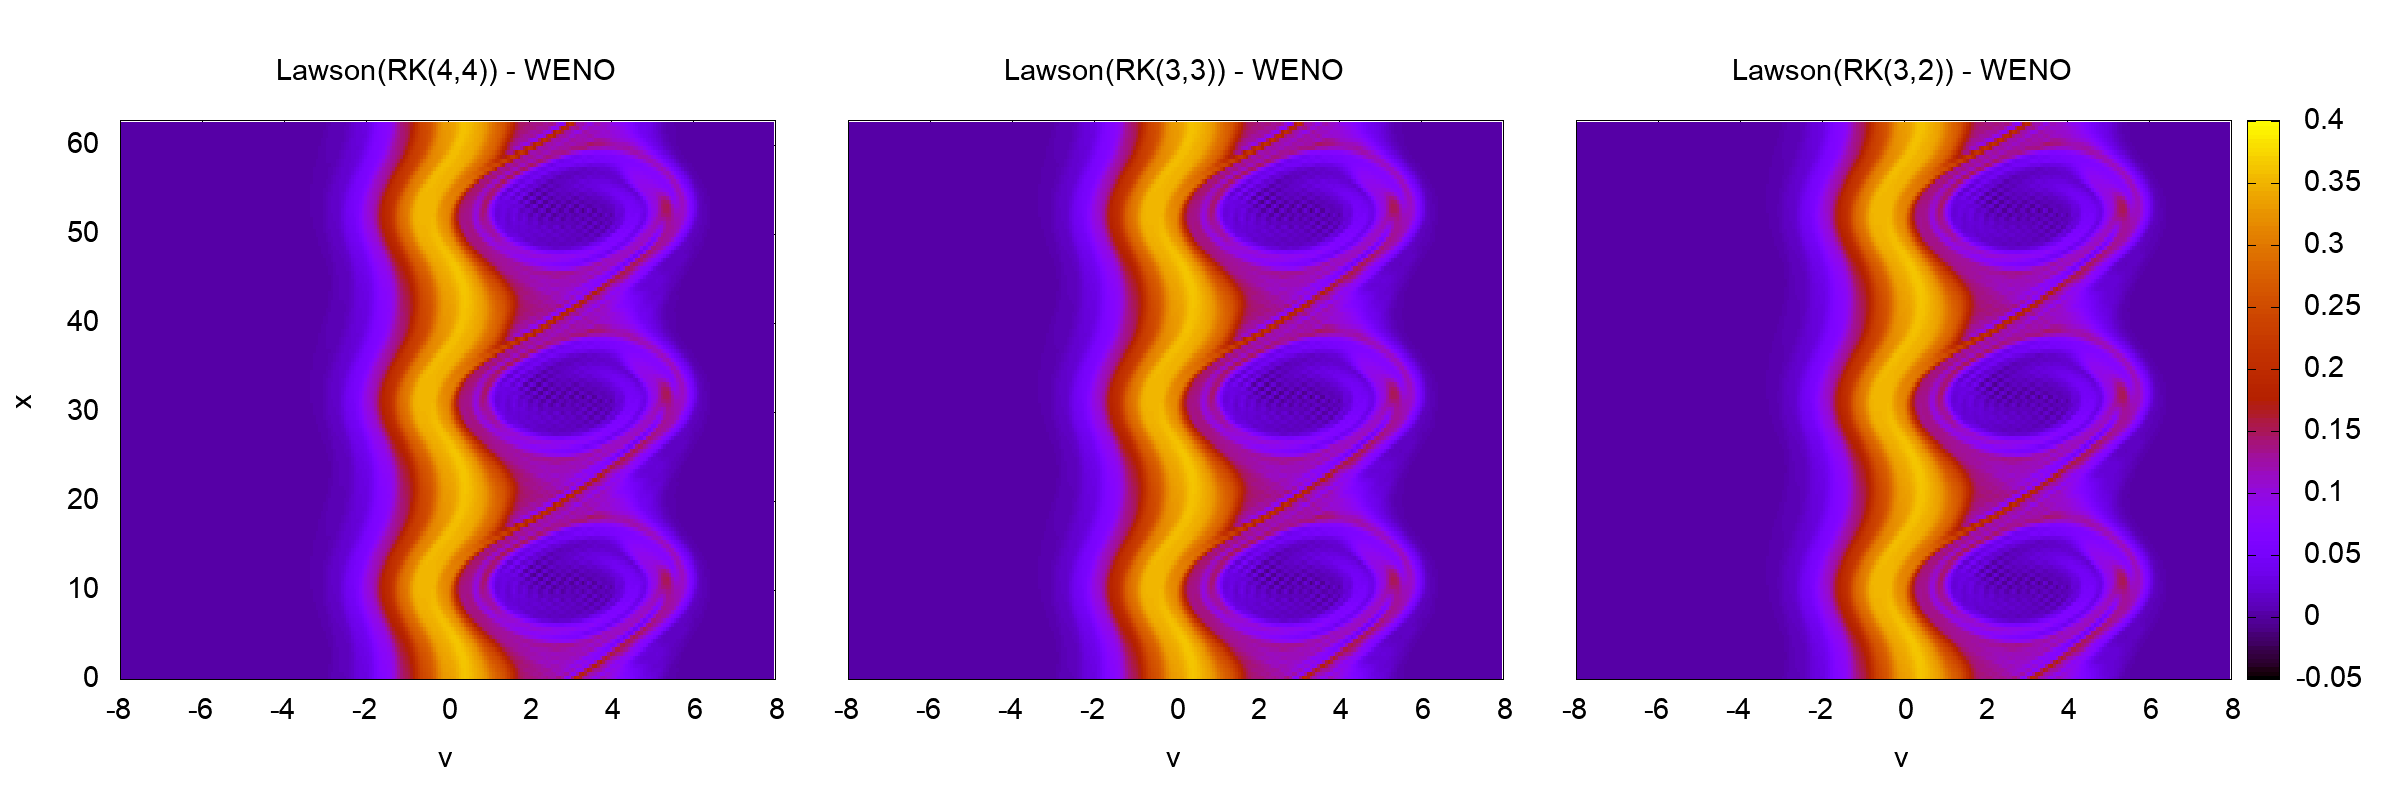
\includegraphics[width=\textwidth]{\localPath/figures/vp_dt0p05_weno.png} \\
    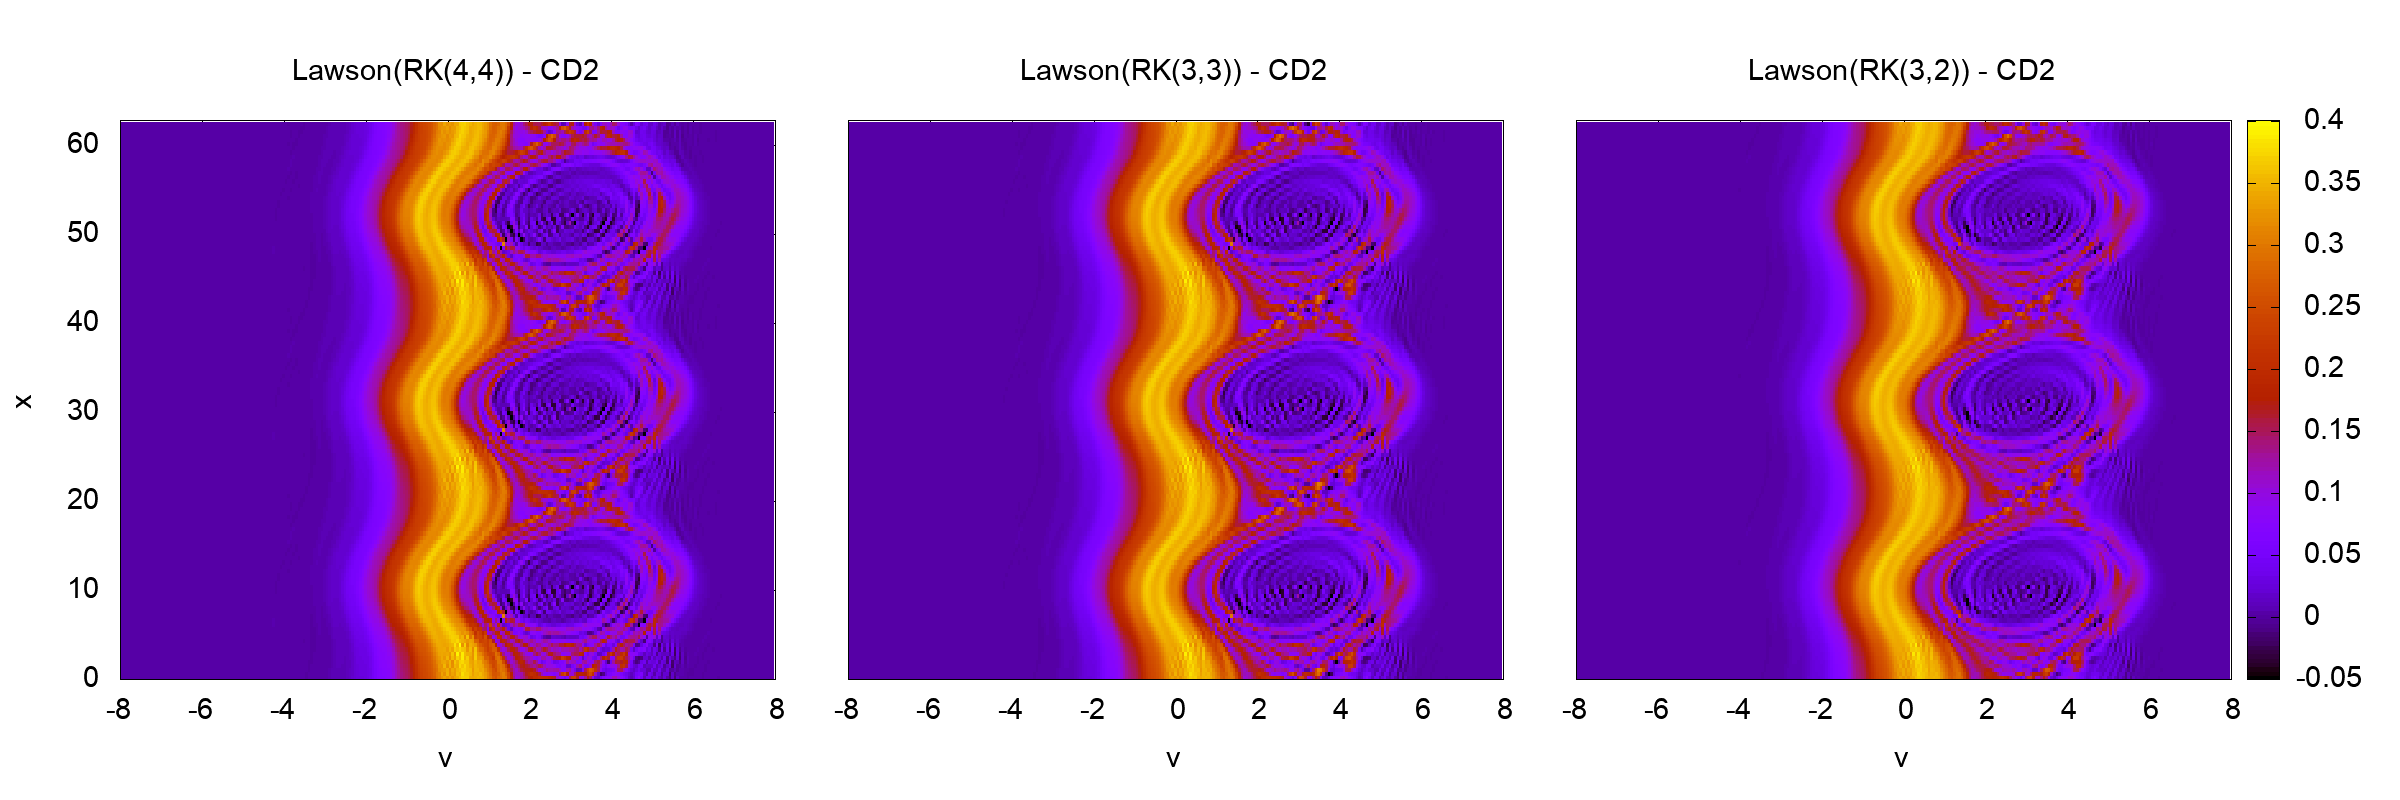
\includegraphics[width=\textwidth]{\localPath/figures/vp_dt0p05_o2.png}\\
    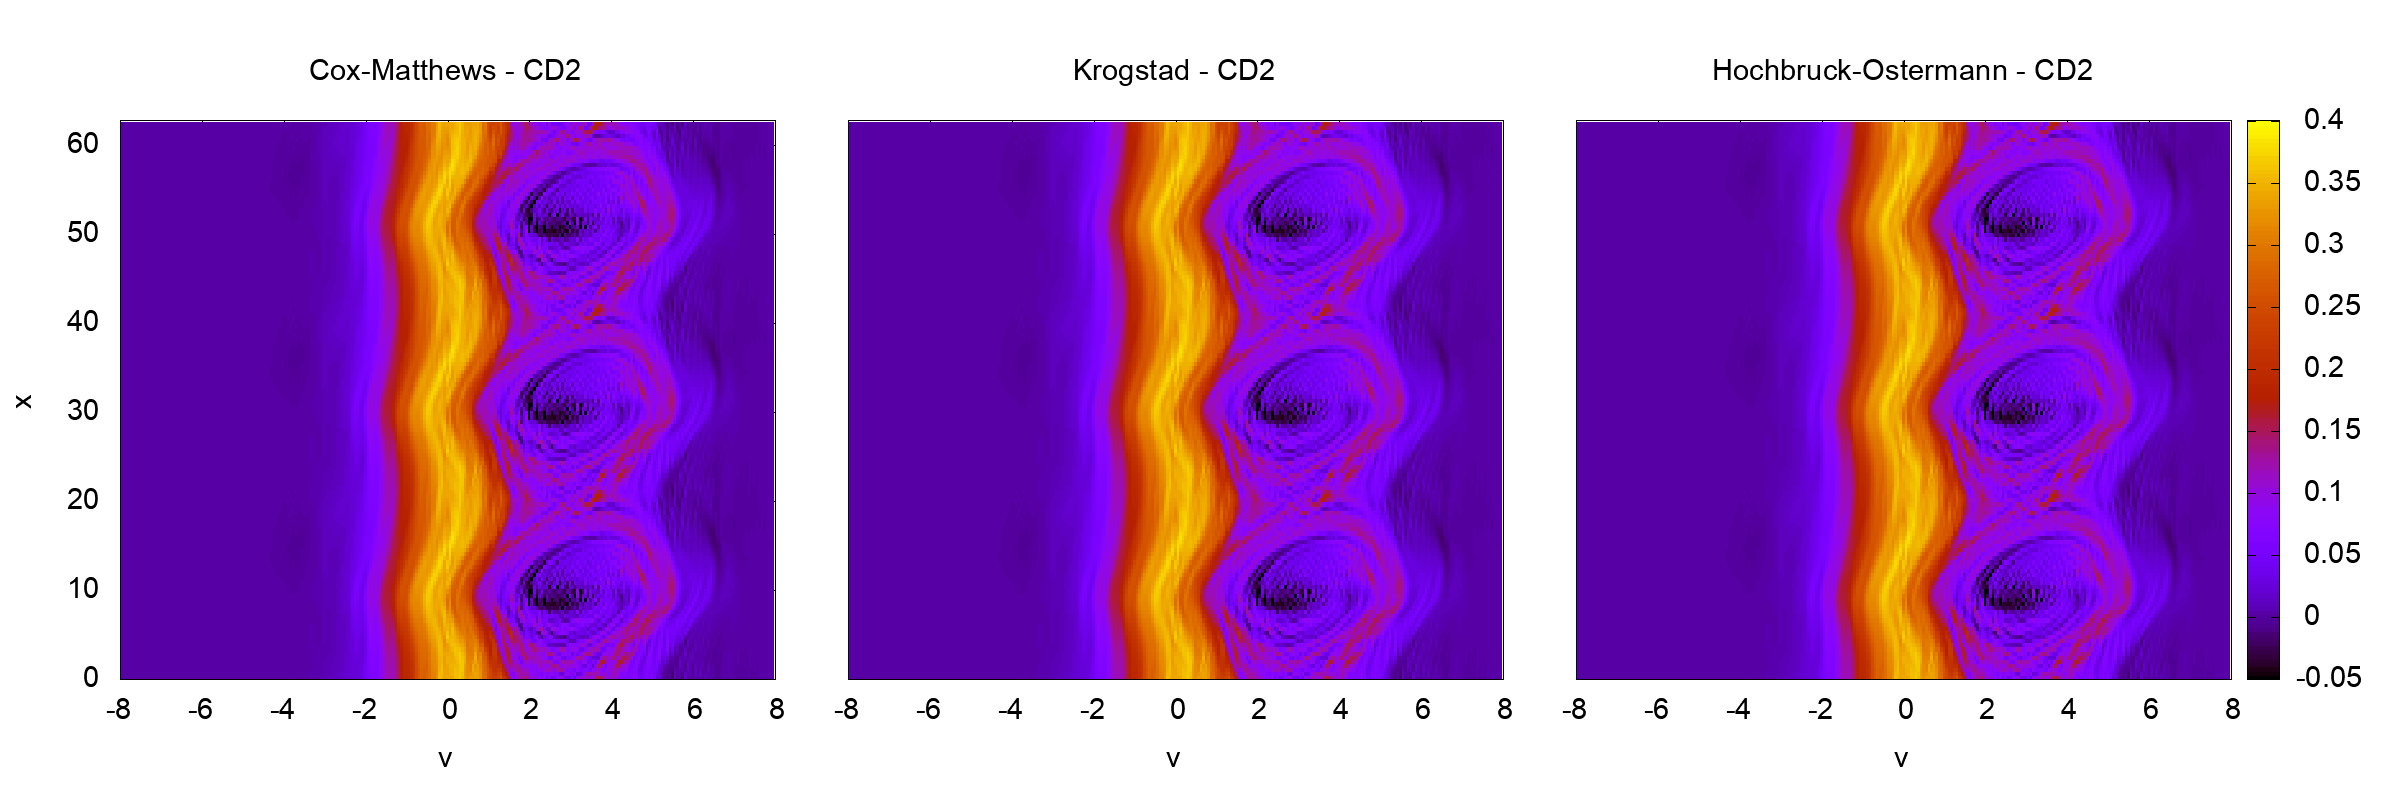
\includegraphics[width=\textwidth]{\localPath/figures/vp_dt0p05_expRK.png}
  \end{tabular}
    \caption{{\color{black} Distribution function at time $t=40$ as a function of $x$ and $v$ for: $(i)$ Lawson schemes ($RK(4, 4)$, $RK(3, 3)$, $RK(3, 2)$) + WENO5 (first row) ; $(ii)$ Lawson schemes ($RK(4, 4)$, $RK(3, 3)$, $RK(3, 2)$) + centered difference scheme (second row) ; $(iii)$ exponential schemes (Cox-Matthews, Krogstad, Hochbruck--Ostermann) + centered difference scheme (third row).}}  
\label{space}      
\end{figure}



%\begin{figure}
%\centering
%    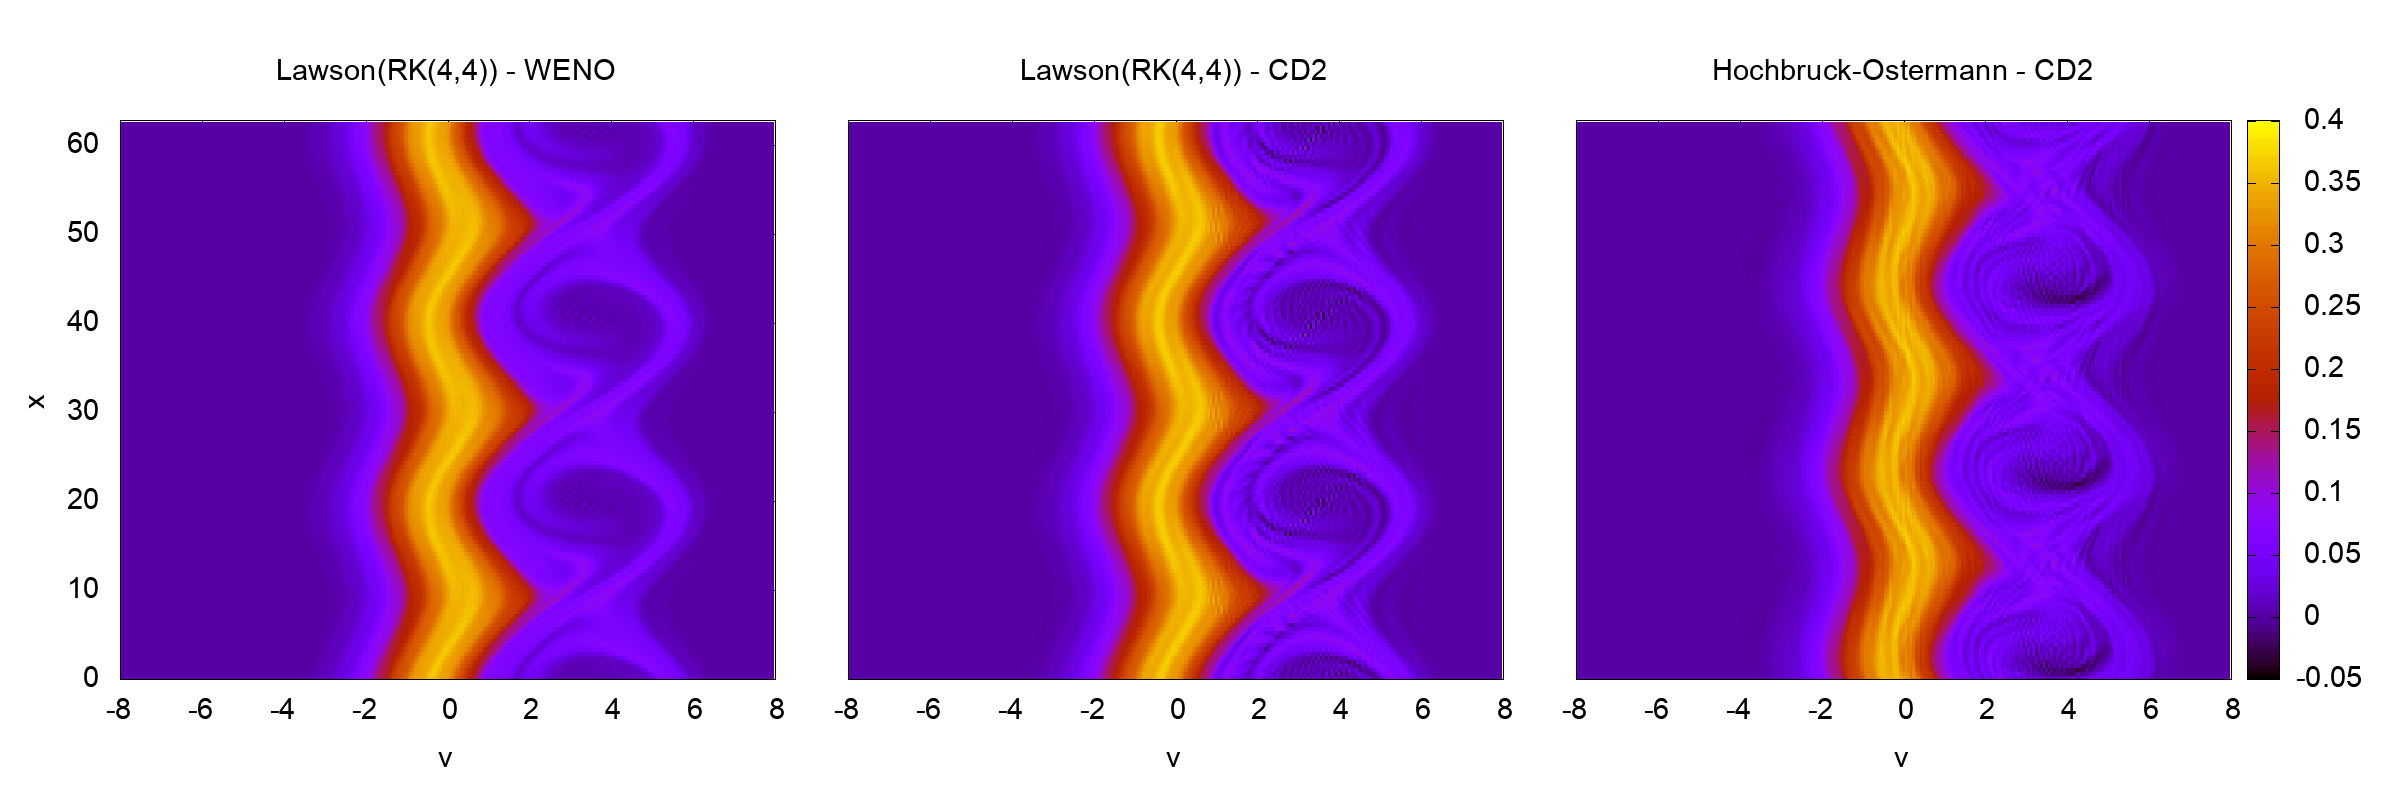
\includegraphics[width=\textwidth]{\localPath/figures/vp_cfl.png}
%    \caption{Distribution function at time $t=40$ as a function of $x$ and $v$ for Lawson($RK(4, 4)$) + WENO5 (left), Lawson($RK(4, 4)$) + centered scheme (center), Hochbruck--Ostermann + centered scheme (right).}  
%\label{space}      
%\end{figure}

In Figure \ref{total_energy}, we plot the time evolution of $({\cal H}^n -{\cal H}(0))/{\cal H}(0)$, where ${\cal H}^n\approx {\cal H}(n\Delta t)$ and ${\cal H}(t)$ is the total energy defined by 
$$
{\cal H}(t) = \frac{1}{2}\int\int |v|^2 f(t, x, v) \,dxdv + \frac{1}{2}\int |E|^2(t, x) \,dx. 
$$
This quantity is known to be preserved with time {\color{black} at the continuous level. It is thus a useful metric to evaluate and compare the different numerical 
methods. At this stage, all the used numerical methods are stable and we now look at their accuracy with respect to conservation of energy. }
% and thus allows us to look at the accuracy of the different methods considered in this paper.
We observe that Lawson/centered schemes (referred as 'CD2' in the 
legend) preserve this quantity well. It is well known (see for example \cite{cf}) that centered schemes are better at preserving the total energy compared to upwind schemes. The reason is that upwind schemes introduce numerical diffusion. The exponential integrators that are considered show all very similar behavior with respect to energy conservation. They seem to include less drift than the Lawson methods, but for the time scales considered here their error is larger.

\begin{figure}%[h]
	\centering
	%\input{\localPath/figures/H}
  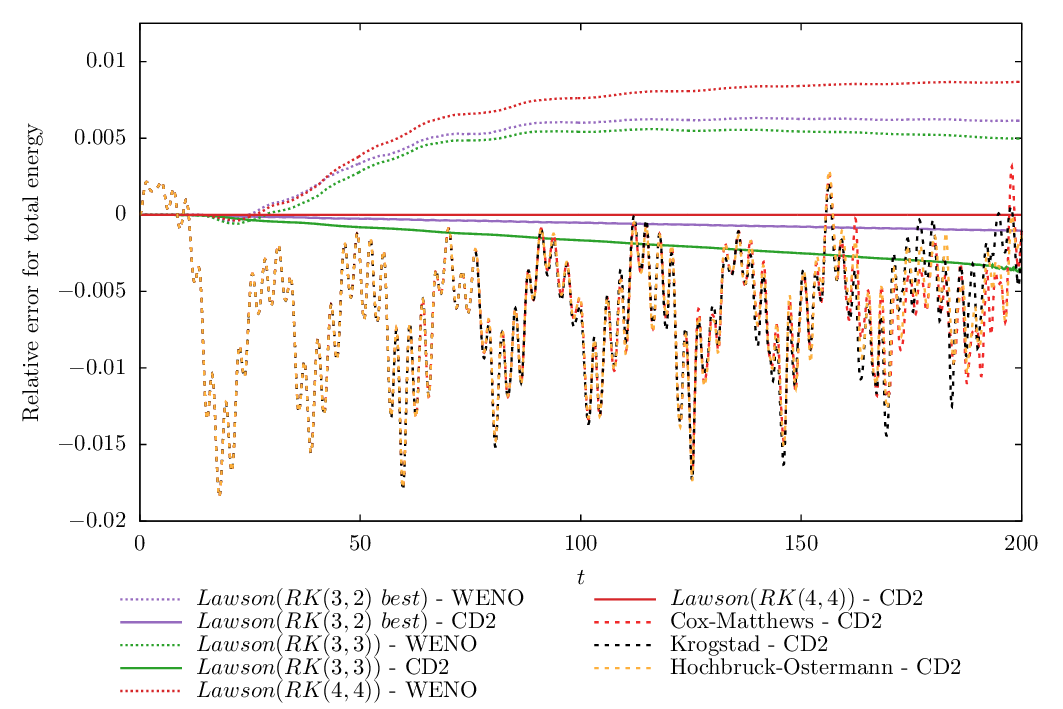
\includegraphics[width=0.9\textwidth]{\localPath/figures/H.png}
	\caption{Time evolution of the relative error of the total energy for the different methods. }
	\label{total_energy}
\end{figure}

Although being able to choose the time step size independently of the mesh is a desirable feature, it makes checking the sharpness of the CFL estimate derived in the previous section more difficult. To accomplish this, we consider the same parameters as before, except for the phase space mesh which now uses $N_x=81$ and $N_v=512$ grid points.  Then the maximum time step becomes $\Delta t=\min_n C\Delta v/\|E^n\|_{L^\infty} \approx 0.052C$ (since $\max_n \|E^n\|_{L^\infty}\approx 0.6$ and $\Delta v=16/512=0.03125$). We consider two different time steps:  $\Delta t=0.052C$ (which satisfies the linearized CFL condition) and $\Delta t = 1.4 \times 0.052C$ (which violates the linearized CFL condition). The results are shown in Figure \ref{unstable}. There the Lawson($RK(4,4)$) method has been chosen for the time discretization whereas WENO5 and centered scheme are both considered for the velocity discretization. More specifically,
\begin{itemize}
    \item for WENO5 we use $C=1.73$ (obtained from the linearized version LW5) and we compare the results obtained 
    with $\Delta t=0.09$ (satisfies the CFL condition) and $\Delta t=0.13$ (does not satisfy the CFL condition). 
    \item for the centered scheme, we use $C=2\sqrt{2}$ and we compare the results obtained with $\Delta t=0.14$ (satisfies the CFL condition) with $\Delta t=0.2$ (does not satisfy the CFL condition). 
\end{itemize}
In Figure \ref{unstable}, the time evolution of the electric energy $\|E(t)\|^2_{L^2}$ is displayed for these two velocity discretizations.  
One can observe for the time step size that satisfies the CFL condition the simulation is stable and gives the expected results, whereas for the choice that violates the CFL condition the simulation blows up. Thus, the results confirm that the CFL condition obtained by the linear theory yields a good prediction for the nonlinear Vlasov--Poisson equation. 
On the right part of Figure \ref{unstable}, the time history of the quantity $C \Delta v/ \|E^n\|_{L^\infty}$ is shown (red) together with the time step size considered for the WENO velocity discretization. The choice $\Delta t=0.13$ (blue line) is larger than the allowed time step size around $t\approx 20$, which explains the numerical instability observed at that point in time. 

\begin{figure}
\centering
\begin{tabular}{cccc}
  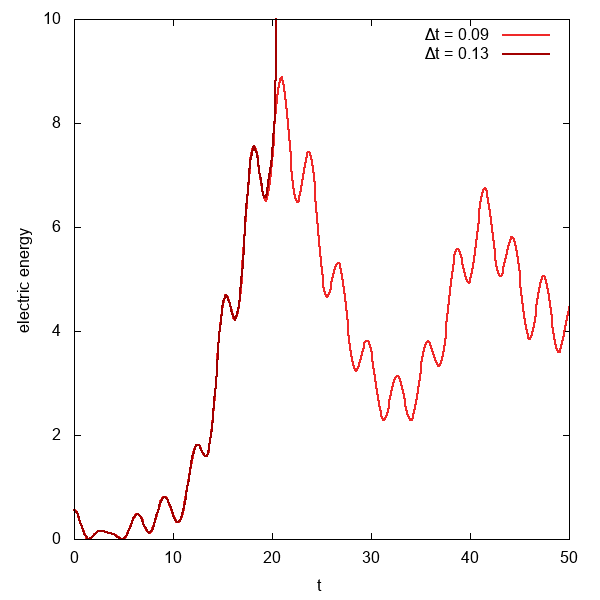
\includegraphics[scale=0.3]{\localPath/figures/ee_weno_rk44.png} &\hspace{-0.2cm}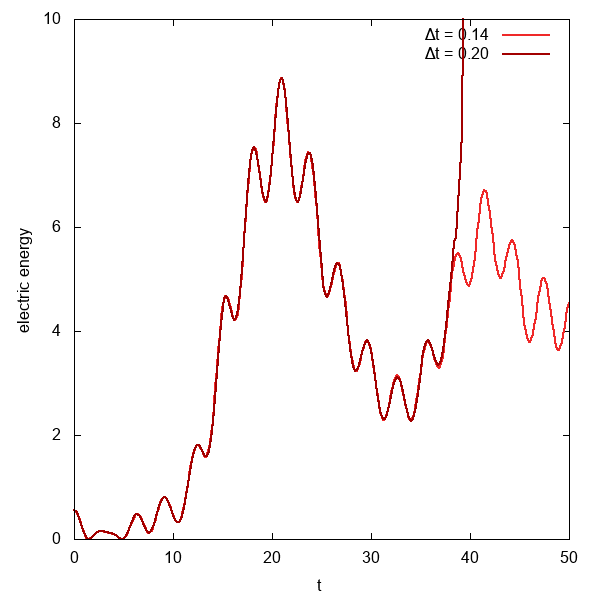
\includegraphics[scale=0.3]{\localPath/figures/ee_o2_rk44.png} & \hspace{-0.2cm}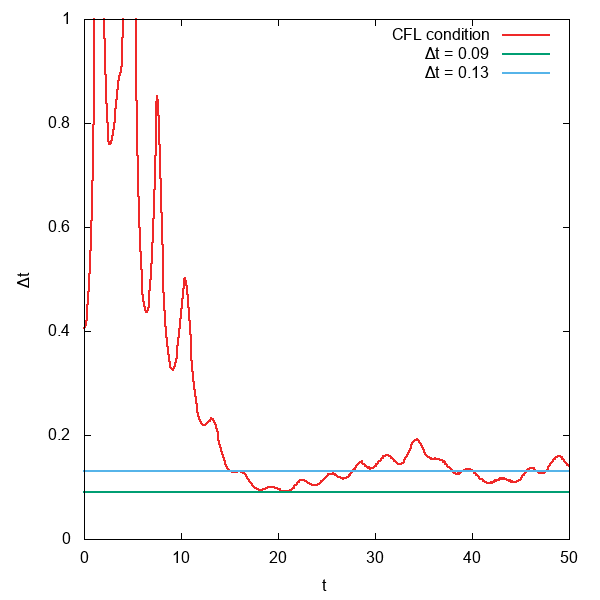
\includegraphics[scale=0.3]{\localPath/figures/bot_cfl_weno_rk44.png} 
   \end{tabular}
\caption{Illustration of the accuracy of the CFL estimate obtained from the linear theory. History of electric energy with Lawson($RK(4,4)$) + WENO5 (left),  Lawson($RK(4,4)$) + centered scheme (middle) and history of CFL condition for Lawson($RK(4,4)$) + WENO5 case (right)}
\label{unstable}      
\end{figure}
 
 
%%%%%%%%%%%%%%%%%%%%%%%%%%%%%
%%%%%%%%%%%%%%%%%%%%%%%%%%%%%
\section{Numerical simulation: drift-kinetic equations \label{sec:dk}}

In this section we will consider a model motivated by the simulation of strongly magnetized plasmas, such as those found in tokamaks. In this case the dynamics is governed by gyrokinetic equations. Gyrokinetics averages out the fast oscillatory motion of the charged particles around the magnetic field lines. In a simplified slab geometry, gyrokinetic models reduce to the drift-kinetic equation. In this case the unknown $f$ depends on three cylindrical spatial coordinates $(r,\theta,z)$ and one velocity direction $v$. This model is composed of a guiding-center dynamics in the plane orthogonal to the magnetic field lines and of a Vlasov type dynamics in the direction parallel (to the magnetic field lines). In addition to its relevance in physics, it is also a good test case for stressing exponential methods. The latter is due to the fact that after some time the nonlinearity can become strong enough such that the time step size is is dictated by stability constraints (especially for high order methods).

Our goal in this section is to find a numerical approximation of $f=f(t,r,\theta,z,v)$ satisfying the following $4D$ slab drift-kinetic equation (see \cite{grandgirard})
\begin{equation}
\label{dk}
\partial_tf-\frac{\partial_\theta \phi}{r}\partial_rf+\frac{\partial_r \phi}{r}\partial_\theta f
+v\partial_zf-\partial_z\phi\partial_{v}f=0,
\end{equation}
for $(r,\theta,z,v)\in \Omega\times[0,L]\times \mathbb{R}$, $\Omega=[r_{\rm min},r_{\rm max}]\times [0, 2\pi]$.
The self-consistent potential $\phi=\phi(r,\theta,z)$ is determined by solving the quasi neutrality equation
\begin{align}
    -\left[\partial_r^2\phi+\left(\frac{1}{r}+\frac{\partial_r n_0(r)}{n_0(r)}\right)\partial_r\phi \right.&+\left.\frac{1}{r^2}\partial_\theta^2\phi\right]+\frac{1}{T_e(r)}(\phi-\langle\phi\rangle)\nonumber\\
\label{qn}
&\hspace{-3cm}=\frac{1}{n_0(r)}\int_{\mathbb{R}} fdv-1,
\end{align}
where $\langle\phi\rangle = \frac{1}{L}\int_0^L \phi(r,\theta,z)\,dz$ and the functions $n_0$ and $T_e$ depend only on $r$ and are given analytically.


In many situations the $v \partial_z f$ term yields the most restrictive CFL condition. In this setting exponential methods can be very successful as they remove the most stringent CFL condition, while still treating the remaining terms explicitly (which computationally is relatively cheap). The $\varphi$ functions can be computed in Fourier space (as has been discussed in some detail for the Vlasov--Poisson system in the previous section) or using a semi-Lagrangian approach. Exponential integrators for the drift-kinetic model have been proposed in \cite{cep}. They compare favorably to splitting schemes and have the advantage that they can be more easily adapted to different models. In \cite{cep} only a second order exponential integrator and the fourth order Cox--Matthews scheme have been considered. Due to the investigations in the present paper we now understand that this is not an ideal choice. Thus, the purpose of this section is to demonstrate that Lawson methods can be more efficient and to further corroborate the results obtained in the previous sections. The difference in stability for Lawson schemes and exponential integrators will be very evident in the numerical simulations that are presented.

\subsection{Numerical discretization}

First, we remark that $z$ is a periodic variable which motivates us to consider the Fourier transform in this direction. The corresponding frequencies are denoted by $k$. Equation \eqref{dk} then becomes
$$
\partial_t \hat{f}_k -\partial_r \widehat{\left(\frac{\partial_\theta \phi}{r}f\right)}_k+\partial_\theta \widehat{\left(\frac{\partial_r \phi}{r} f\right)}_k +vik \hat{f}_k-\partial_v\widehat{\left( \partial_z\phi \, f\right)}_k=0, 
$$
Setting $F(t, f)= \partial_r \widehat{\left(\frac{\partial_\theta \phi}{r}f\right)}-\partial_\theta \widehat{\left(\frac{\partial_r \phi}{r} f\right)} +\partial_v\widehat{\left( \partial_z\phi \,f\right)}$, this equation can be written as
$$
\partial_t \hat{f} = - vik \hat{f} + F(t, f). 
$$
This is now precisely in the form to which we can apply an exponential method. In addition, computing the required matrix functions is very efficient as all the frequencies decouple (see the corresponding discussion in section \ref{sec:vp}).

To complete the numerical scheme, one has to detail the phase space approximation. As in \cite{cep} we will use Arakawa's method to approximate the derivatives needed to compute $F$. Arakawa's method is a centered difference scheme that conserves three invariants. More details can be found in \cite{cep}.


\subsection{Numerical results \label{subsec:driftkinetic-results}}

In this section, we detail the physical parameters of the considered test case. The set up is identical to \cite{cep} (see also 
\cite{BC2013, vlasovia}). The initial value is given by 
\begin{align*}
f(t=0,r,\theta,z,v) &=
f_{\rm eq}(r,v)\left[1+\epsilon \exp\left(-\frac{(r-r_p)^2}{\delta r}\right)\cos\left(\frac{2\pi n}{L}z+m\theta\right)\right],
\end{align*}
where the equilibrium distribution is given by
\begin{equation} \label{eq:equilibrium}
f_{\rm eq}(r,v)=\frac{n_0(r)\exp(-\frac{v^2}{2T_i(r)})}{(2\pi T_i(r))^{1/2}}.
\end{equation}
The radial profiles $T_i$, $T_e$, and $n_0$ have the analytic expressions
$$
\mathcal{P}(r) = C_\mathcal{P}\exp\left(-\kappa_\mathcal{P}\delta r_{\mathcal{P}}\tanh(\frac{r-r_p}{\delta r_{\mathcal{P}}})\right), \; \mathcal{P}\in \{T_i,T_e,n_0\}
$$
with the constants defined as follows
$$
\ C_{T_i}=C_{T_e}=1,\ C_{n_0}=\frac{r_{\rm max}-r_{\rm min}}{
\int_{r_{\rm min}}^{r_{\rm max}}\exp(-\kappa_{n_0}\delta r_{n_0}\tanh(\frac{r-r_p}{\delta r_{n_0}}))\,dr}.
$$
Finally, we consider the parameters of \cite{BC2013} (MEDIUM case)
\begin{eqnarray*}
&&r_{\rm min} = 0.1,\ r_{\rm max} = 14.5,\\
&& \kappa_{n_0}= 0.055,\ \kappa_{T_i}=\kappa_{T_e}= 0.27586,\\
&&\delta r_{T_i}=\delta r_{T_e}=\frac{\delta r_{n_0}}{2}= 1.45,\ \epsilon=10^{-6},\ n=1,\ m=5,\\
&&L=1506.759067,\ r_p = \frac{r_{\rm min}+r_{\rm max}}{2},\delta r = \frac{4 \delta r_{n_0}}{\delta r_{T_i}}.
\end{eqnarray*}
and use a $v$-range of $v \in [-7.32,7.32]$.

We consider two configurations. A direct formulation, where the boundary conditions are given by
$$
f(r_{\rm min},\theta ,z,v)=f_{eq}(r_{\rm min},v) \qquad
f(r_{\rm max},\theta ,z,v)=f_{eq}(r_{\rm max},v).
$$
Note that these are not homogeneous Dirichlet boundary conditions. It is well known (and supported by \cite{cep}) 
that the Arakawa scheme works better for homogeneous boundary conditions. In addition to the direct formulation, we therefore also introduce a so-called perturbation formulation (see also \cite{vlasovia, latu2}).
First, we note that the equilibrium function $f_{\rm eq}$ defined in (\ref{eq:equilibrium}) is a steady state for our problem. We therefore divide $f$ into
$$
f(t,r,\theta ,v)=f_{eq}(r,v)+\delta f(t,r,\theta ,v).
$$
With this formulation, our problem (\ref{dk}) becomes
$$
\partial_t\delta f+\frac{E_\theta}{r}\partial_r (f_{eq} + \delta f)-\frac{E_r}{r}\partial_\theta \delta f+v\partial_z\delta f+E_z \partial_v (f_{eq} + \delta f)=0,
$$
where $E_\theta=-\partial_\theta \phi$, $E_r=-\partial_r \phi$ and $E_z=-\partial_z \phi$. Expanding the various terms we obtain
$$
\partial_t\delta f+\frac{E_\theta}{r}\partial_r\delta f-\frac{E_r}{r}\partial_\theta \delta f+v\partial_z\delta f+ E_z \partial_v \delta f
+\frac{E_\theta}{r}\partial_r f_{eq} + E_z \partial _v f_{eq}=0
$$
which can be written as
$$
\partial_t\delta f + v\partial_z \delta f -F(\delta f) +\frac{E_\theta}{r}\partial_r f_{eq} +E_z\partial _v f_{eq} = 0.
$$
Note that the equation is very similar to equation (\ref{dk}). We, however, have obtained two additional source terms, which depend on the equilibrium distribution $f_{eq}$ as well as on the electric field.
Furthermore, the right hand side of the quasi-neutrality equation (\ref{qn}) becomes
$$
\frac{1}{n_0}\int f_{eq} \,dv+\frac{1}{n_0}\int \delta f \,dv-1 = \frac{1}{n_0}\int \delta f \,dv.
$$
Due to the similarity of the direct formulation and the perturbation formulation, the same code can 
be used for both by simply exchanging the right hand side of the quasi-neutrality equation, changing the boundary conditions, and adding the appropriate source terms. Thus, to implement the exponential integrator we consider the following equation 
$$ \partial_t\delta f + v\partial_z \delta f  = F_{pert}(\delta f),  $$
with
$$ F_{pert} (\delta f)= F(\delta f) -\frac{E_\theta}{r}\partial_r f_{eq} - E_z\partial _v f_{eq},  $$
and proceed as before (with $F$ replaced by $F_{pert}$). The space discretization of the source terms can be done either analytically or using a numerical approximation. In our implementation we have used standard centered differences. The Arakawa scheme that is used to discretize $F(\delta f)$ now employs homogeneous Dirichlet boundary conditions for $\delta f$ in the $r$-direction.

We have seen in section \ref{sec:vp} that for the Vlasov--Poisson equation we can derive a constraint on the time step size which ensures stability. 
For Lawson methods this also gives a good estimate in practice. However, for exponential integrators the situation is far more complicated, see the discussion in section \ref{ode}. Thus, a natural question that arises is how large time steps can we take in practice. To do that we will employ an adaptive step size controller that uses Richardson extrapolation to obtain an error estimate. By denoting a time step as follows $f^{n+1} = \varphi_{\Delta t_n}(f^n)$ and considering 
$\tilde{f}^{n+1} = \varphi_{\Delta t_n/2}\circ \varphi_{\Delta t_n/2}(f^n)$
we can construct the Richardson extrapolated numerical solution of a method of order $p$ as follows
$f_R^{n+1} = (2^{p+1} \tilde{f}^{n+1} - f^{n+1})/(2^{p+1} -1)$, which turns out 
to be an approximation of order $(p+1)$ of the exact solution.  
Then, it is possible to determine an estimate of the local error 
$e_{n+1}$ 
of the time integrator through the following expression 
$$
e_{n+1} = \left\Vert f_R^{n+1} - f^{n+1}\right\Vert_{L^{\infty}} + {\cal O}(\Delta t_n^{p+2}), 
%\left\Vert \frac{2^{p+1} (\tilde{f}^{n+1} - f^{n+1})}{2^{p+1}  - 1} - f^{n+1} \right\Vert_{L^2} + {\cal O}(\Delta t_n^{p+2}), 
$$
where the $L^\infty$ norm is considered in the $r, \theta, z, v$ variables. If the estimate for the error $e_{n+1}$ is larger than a specified $\text{tol}$ we reject the step and start again from time $t_n$. Otherwise, the step is accepted and we proceed with the time integration. In either case we then determine the new step size $\Delta t_{new}$ such that the local error is smaller than the tolerance. That is, we choose 
\begin{equation} 
\label{compute_dt}
\Delta t_{new}=s \Delta t_{n}\left(\frac{\text{tol}}{e_{n+1}}\right)^{1/(p+1)}, 
\end{equation}
where $\text{tol}$ is the prescribed tolerance, $p$ is the order of the method, and $s=0.8$ is a safety factor. This process is very well established in the literature and we refer the interested reader to \cite{gustafsson1988,gustafsson1994,soderlind2002,soderlind2006,lukas}. 
Other strategies can also be considered such as embedded Lawson or exponential methods (see \cite{gni, balac}).  
Such methods may be more efficient but we restrict ourselves here to the strategy based on Richardson extrapolation 
since it can be applied to any time integrator.

An interesting property of this adaptive step size controller is that it forces the time step size to satisfy the stability constraint of the numerical method. This is perhaps surprising at first sight since the scheme only controls the local error. However, numerical instability are characterized by error amplification as integration proceeds in time. Thus, a single step can violate the stability constraint, but later on the error amplification increases the local error in such a way that the adaptive step size controller is forced to reduce the time step size. Thus, the controller ensures that we obtain a stable numerical simulation for which the local error is below the specified tolerance.

This procedure allows us to perform a fair comparison between Lawson methods and exponential integrators. Since we are mainly interested in the stability of the methods and, particularly in the nonlinear regime, prescribing a stringent tolerance is infeasible in any case, we will choose a relatively large tolerance for our simulation ($\text{tol}=10^{-2}$ for the perturbation formulation). To avoid the problem of too large time steps at the beginning of the simulation, where accuracy and not stability dictates the time step, we limit the maximal step size to 
$\Delta t=11$ (coarse) and $\Delta t=10$ (fine) for second order methods, $\Delta t=30$ for third order methods and Lawson($RK(3, 2) \; best$), 
and $\Delta t=40$ for fourth order methods.

To evaluate the performances of the different time integrators, we consider the time evolution of the electric energy defined by
$$
{\cal E}(t) = \left( \int_{0}^{L} \int_0^{2\pi} \phi^2(t, r_p, \theta, z ) \,d\theta dz \right)^{1/2}, \;\;\; \mbox{ with } r_p=\frac{r_{\min}+r_{\max}}{2}, 
$$
as well as the time evolution of the total mass and the total energy 
\begin{eqnarray*}
{\cal M}(t) &=& \int_{r_{\min}}^{r_{\max}} \int_{0}^{L} \int_0^{2\pi} \int_{\mathbb R} f(t, r, \theta, z, v ) \,dv d\theta dz dr, \nonumber\\ 
{\cal N}(t) &=&\int_{r_{\min}}^{r_{\max}} \int_{0}^{L} \int_0^{2\pi} \int_{\mathbb R} \frac{v^2}{2} f(t, r, \theta, z, v ) \,dv d\theta dz dr \nonumber\\ 
&& + \int_{r_{\min}}^{r_{\max}} \int_{0}^{L} \int_0^{2\pi} \int_{\mathbb R} f(t, r, \theta, z, v )\phi(t, r, \theta, z) \,dv d\theta dz dr. 
\end{eqnarray*}
The numerical results for the perturbation formulation are given in Figure \ref{fig:driftkinetic-pert1}. There
the time history of the electric energy and the time step size as of function of time for two different 
discretizations in phase space, $32 \times 32 \times 32 \times 64$ and  $64 \times 64 \times 64 \times 128$ grid points, are shown. 
We first see that all the time integrators agree very well; that is, we see an initial exponential growth (the rate is in good agreement with the linear theory; see, for example, \cite{BC2013}) 
in the electric energy. This phase is followed by saturation at very similar levels for all numerical methods used. 
We also observe that all exponential integrators, except the method of Krogstad, are forced to reduce their step size after time $t\approx 5000$ for the fine, \ie $64\times 64 \times 64 \times 128$ grid points, case. 
This is particularly drastic for ExpRK33 and the Cox--Matthews method which suffer from stability issues even for the coarse discretization. In general, for the finer space discretization (see the right plot in Figure \ref{fig:driftkinetic-pert1}), the problem becomes significantly more severe. It is also worth mentioning that ExpRK33 leads to unstable results in spite of the step size controller, which clearly highlights the unstable nature of that integrator. 
Neither of the Lawson schemes have similar issues and the size of the stability domain on the imaginary axis gives a good indication of the relative time steps this methods can take. We also note that at later times Lawson schemes are able to take significantly larger time steps compared to exponential integrators. 
The only exponential integrator that performs well in this regime is the method of Krogstad. Thus, the numerical results agree well with what we would expect based on the theoretical analysis. 


\begin{figure}[h]
	\centering
	\begin{subfigure}[b]{0.48\textwidth}
%       \centering 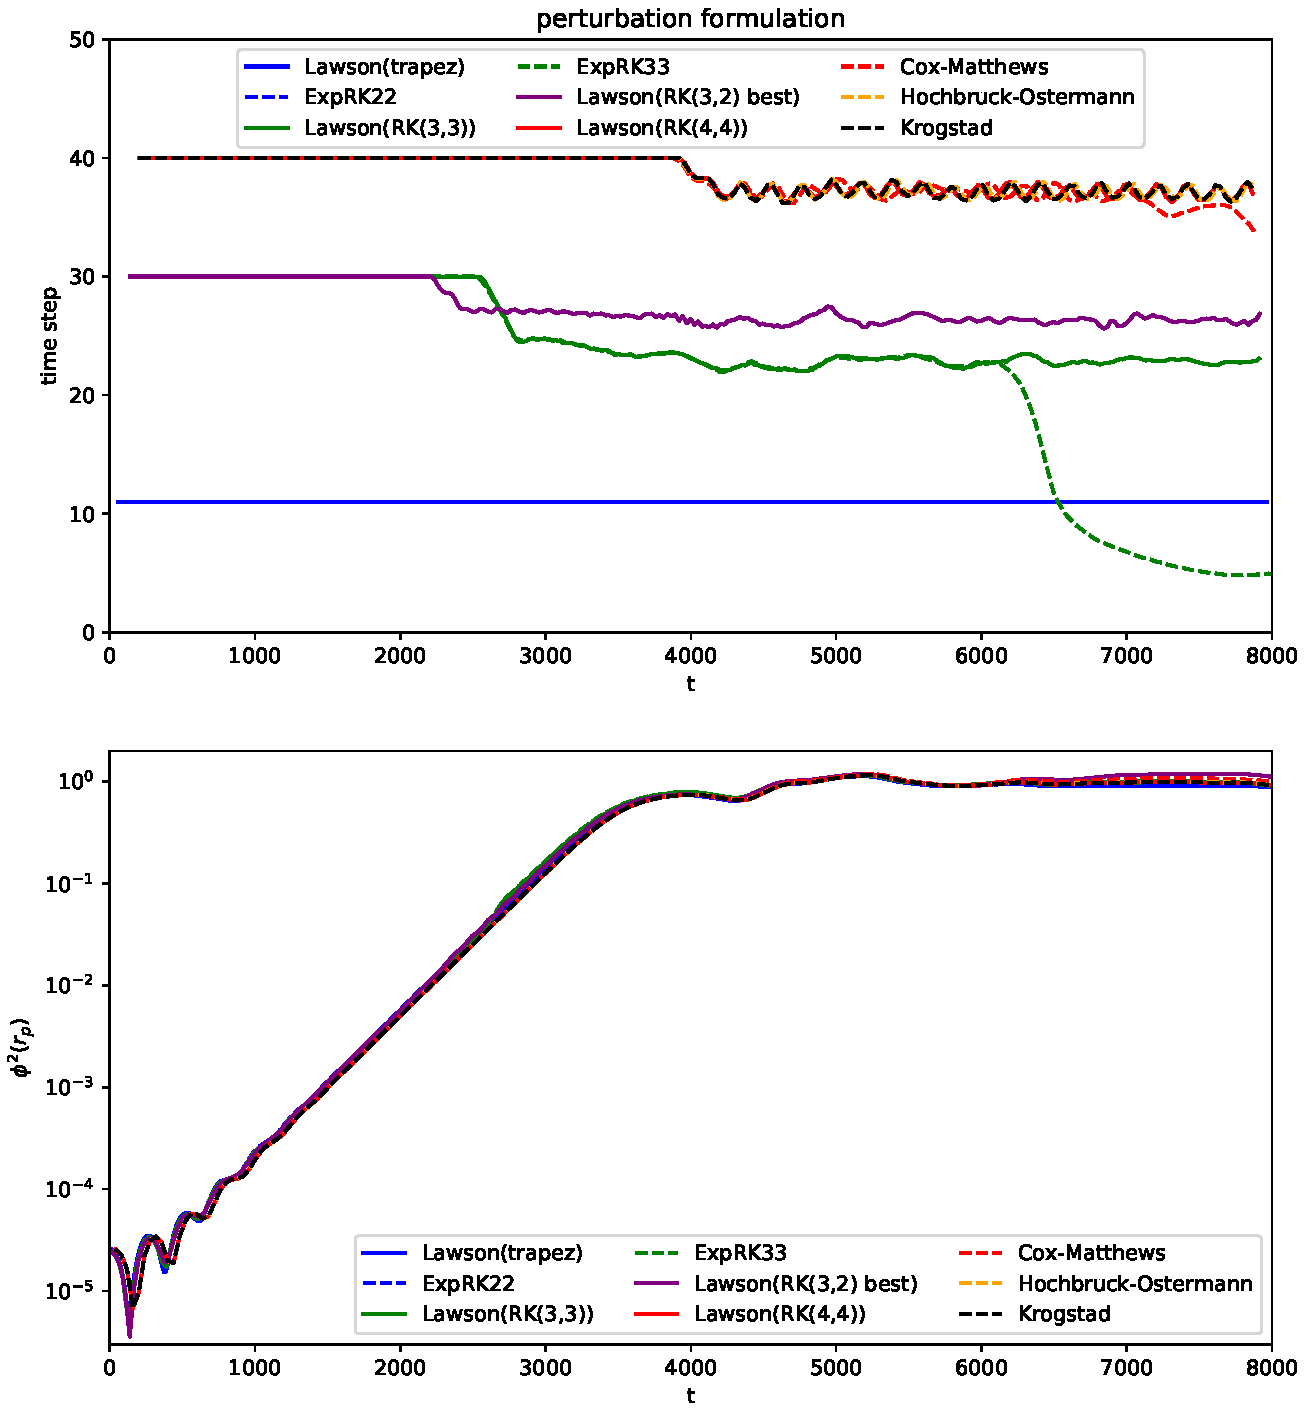
\includegraphics[width=\textwidth]{\localPath/figures/driftkinetic-tol1.00e-02-32x32x32x64-pert1}.pdf
        \centering 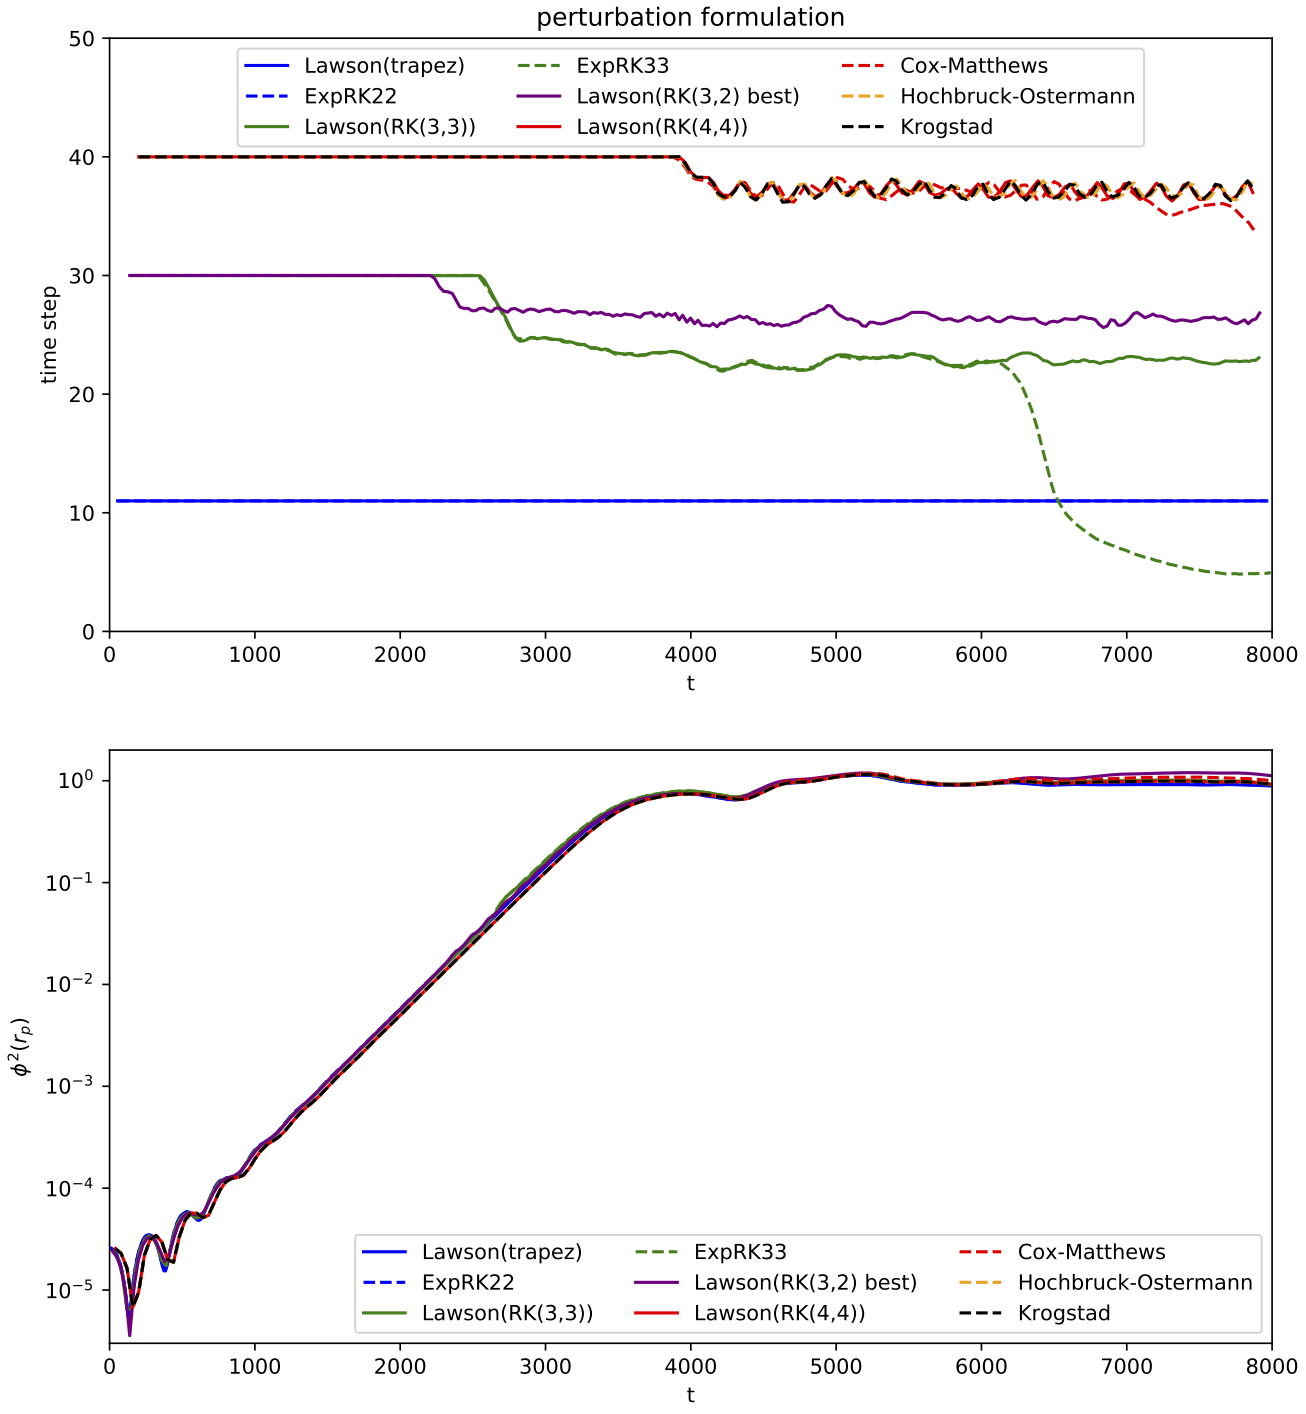
\includegraphics[width=\textwidth]{\localPath/figures/driftkinetic-tol1e-02-32x32x32x64-pert1}%.pdf
	\end{subfigure}
	\begin{subfigure}[b]{0.48\textwidth}
%       \centering 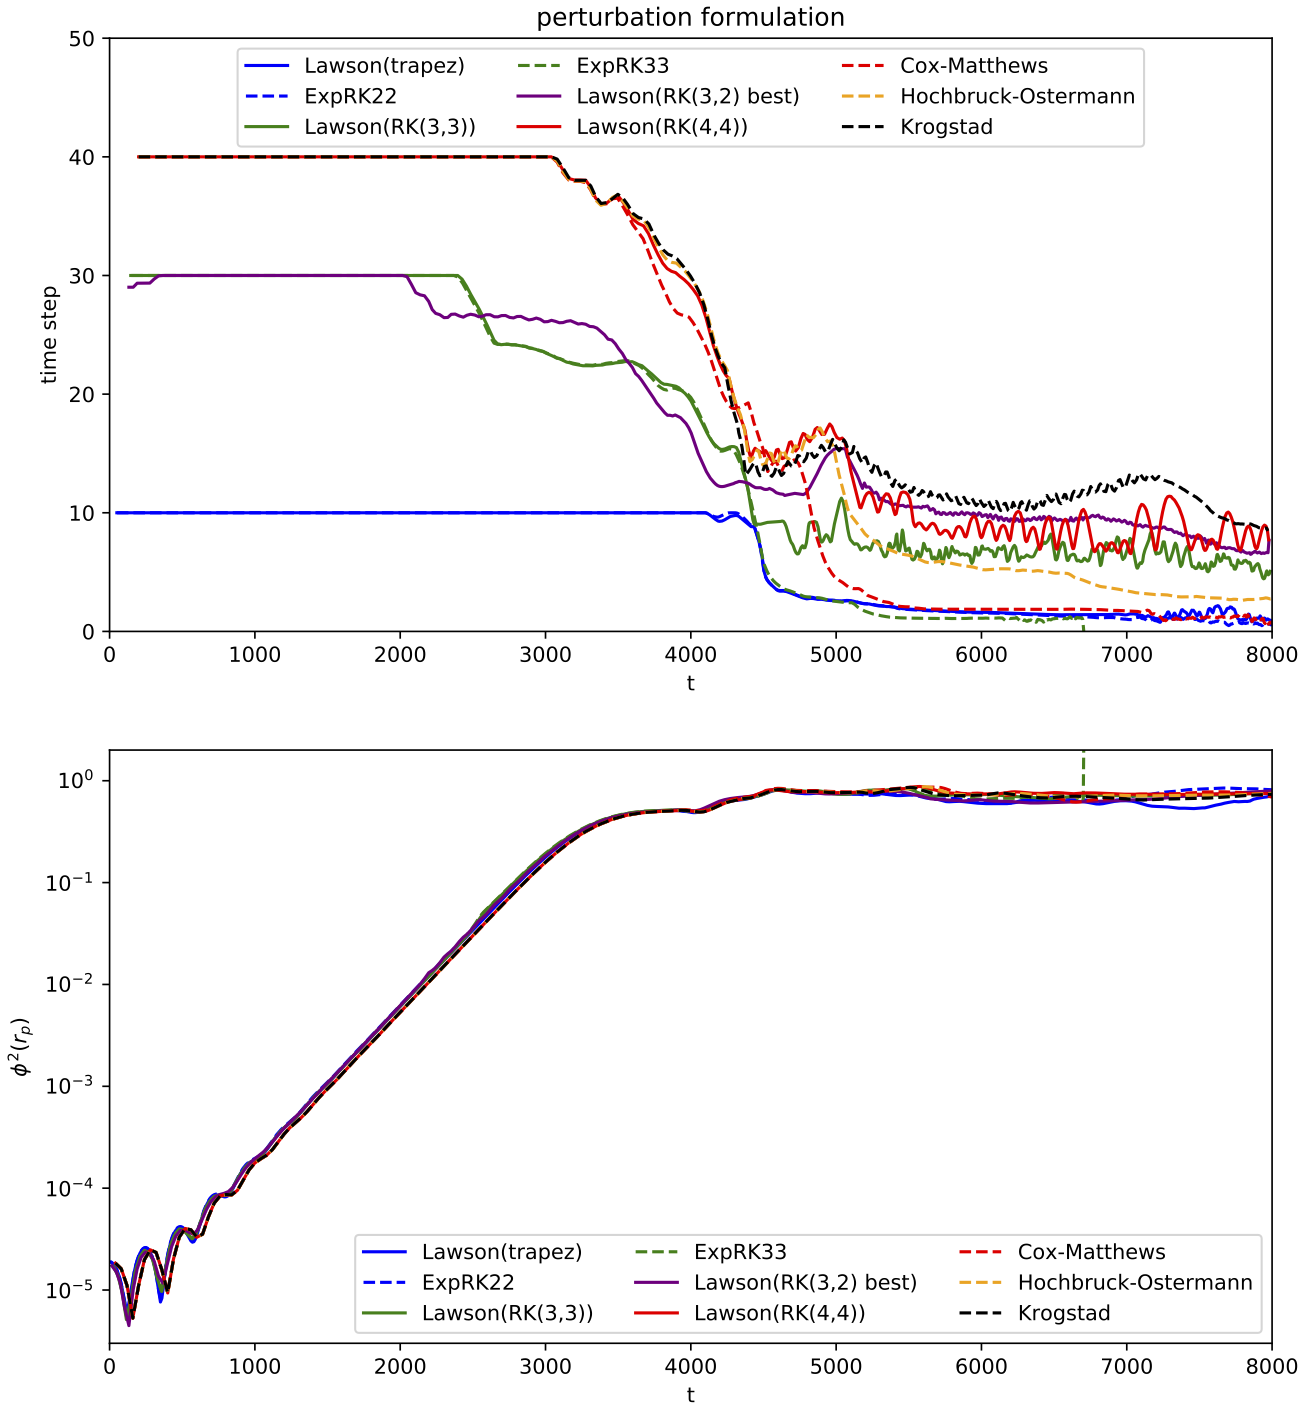
\includegraphics[width=\textwidth]{\localPath/figures/driftkinetic-tol1.00e-02-64x64x64x128-pert1}.pdf
        \centering 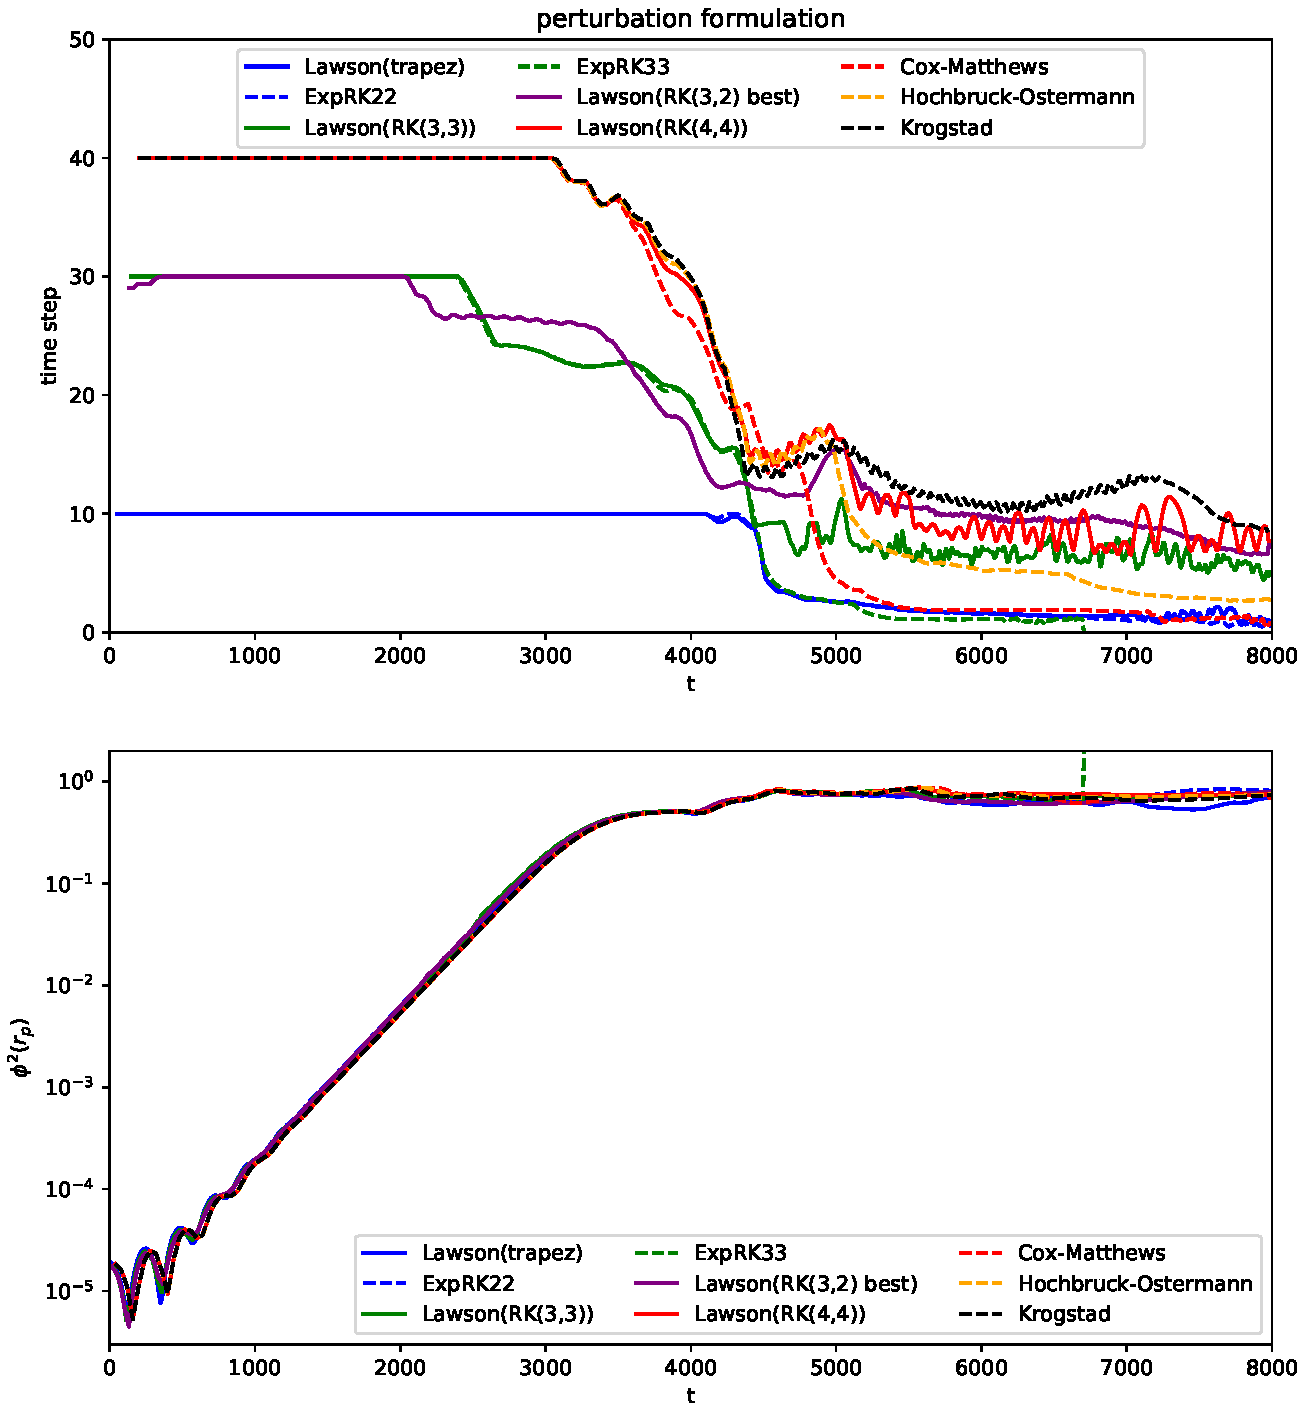
\includegraphics[width=\textwidth]{\localPath/figures/driftkinetic-tol1e-02-64x64x64x128-pert1}%.pdf
	\end{subfigure}
    \caption{Numerical simulation for a number of Lawson methods and exponential integrators for the drift-kinetic model (perturbation formulation). The upper plots show the time step size as a function of time. The lower plots show the time evolution of the electric energy. The configuration on the left uses $32 \times 32 \times 32 \times 64$ grid points and the configuration on the right uses $64 \times 64 \times 64 \times 128$ grid points.}\label{fig:driftkinetic-pert1}
\end{figure}

The corresponding numerical results using the direct formulation are shown in Figure \ref{fig:driftkinetic-pert0}. The situation for the direct formulation is very similar to the perturbation formulation, even if one 
can observe that the time steps are slightly larger than in the perturbation formulation. 
One explanation comes from the fact that the relative error computed in the perturbation 
case involves the norm of $\delta f$ which can be quite different from the norm 
of $f$ so that equation \eqref{compute_dt} leads to different value of the time step 
even if the accuracy of the solution is the same.


\begin{figure}[h]
	\centering
	\begin{subfigure}[b]{0.48\textwidth}
%       \centering 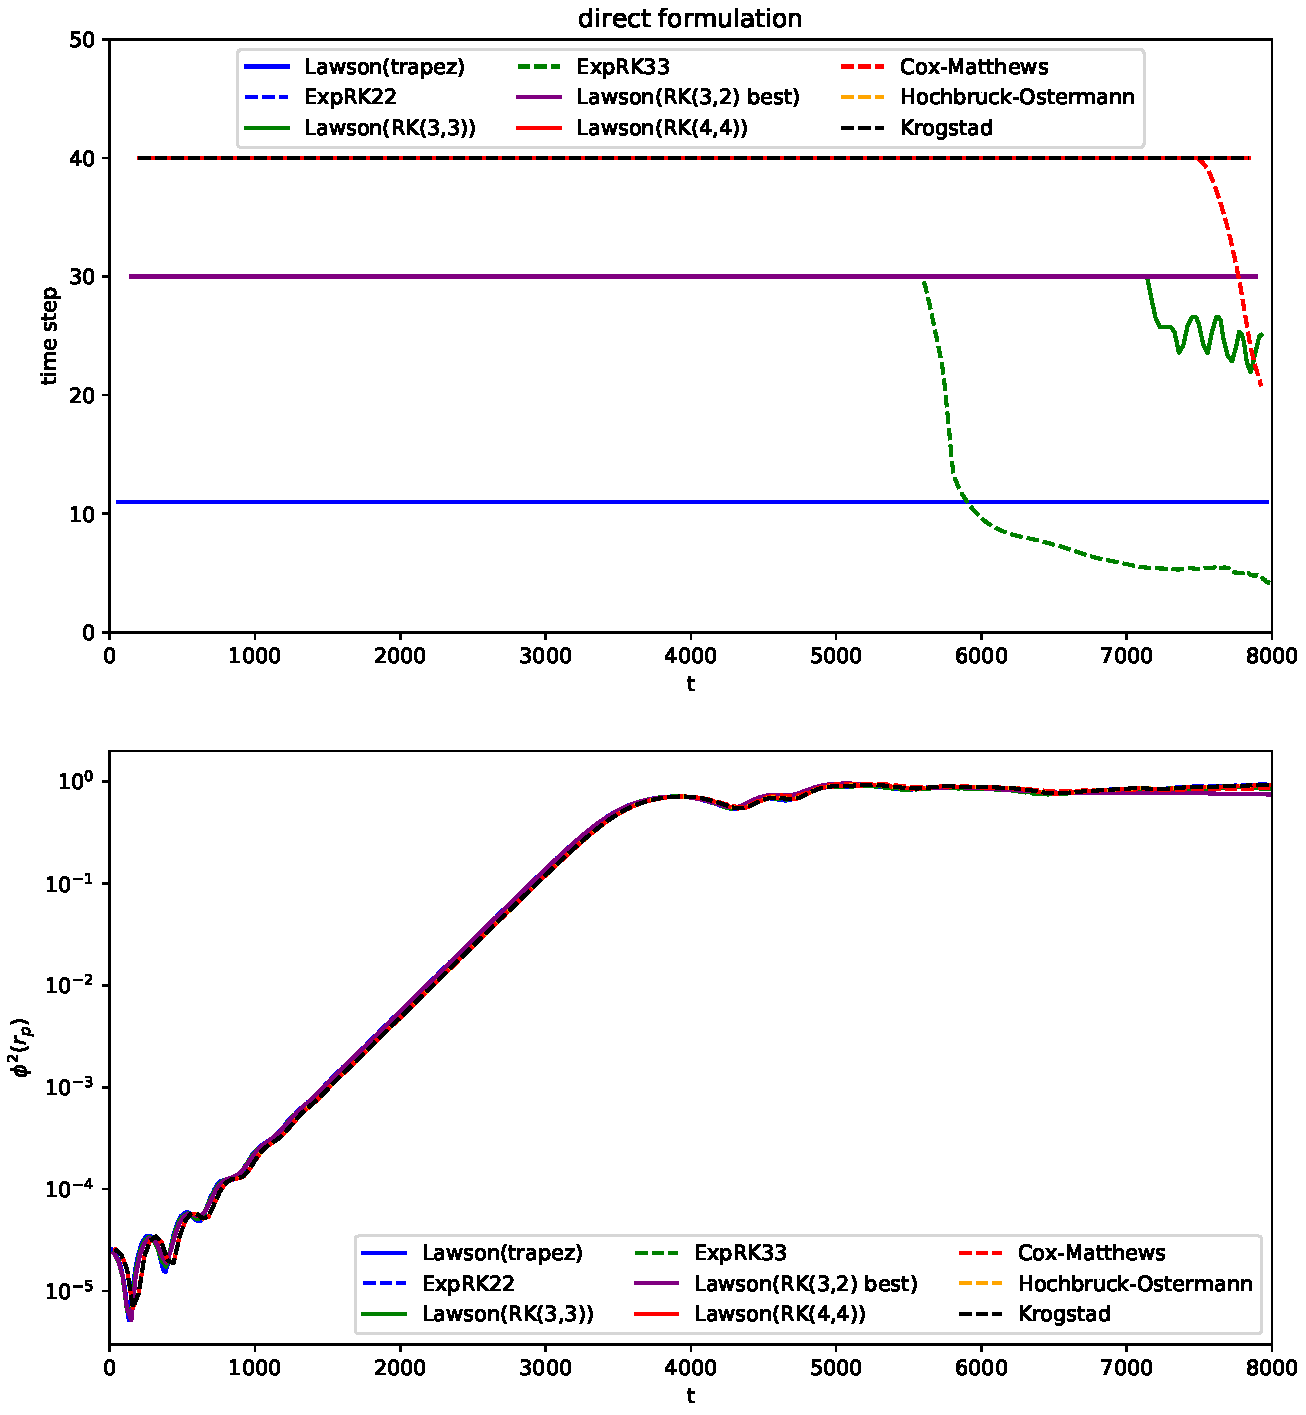
\includegraphics[width=\textwidth]{\localPath/figures/driftkinetic-tol1.00e-02-32x32x32x64-pert0.pdf}
        \centering 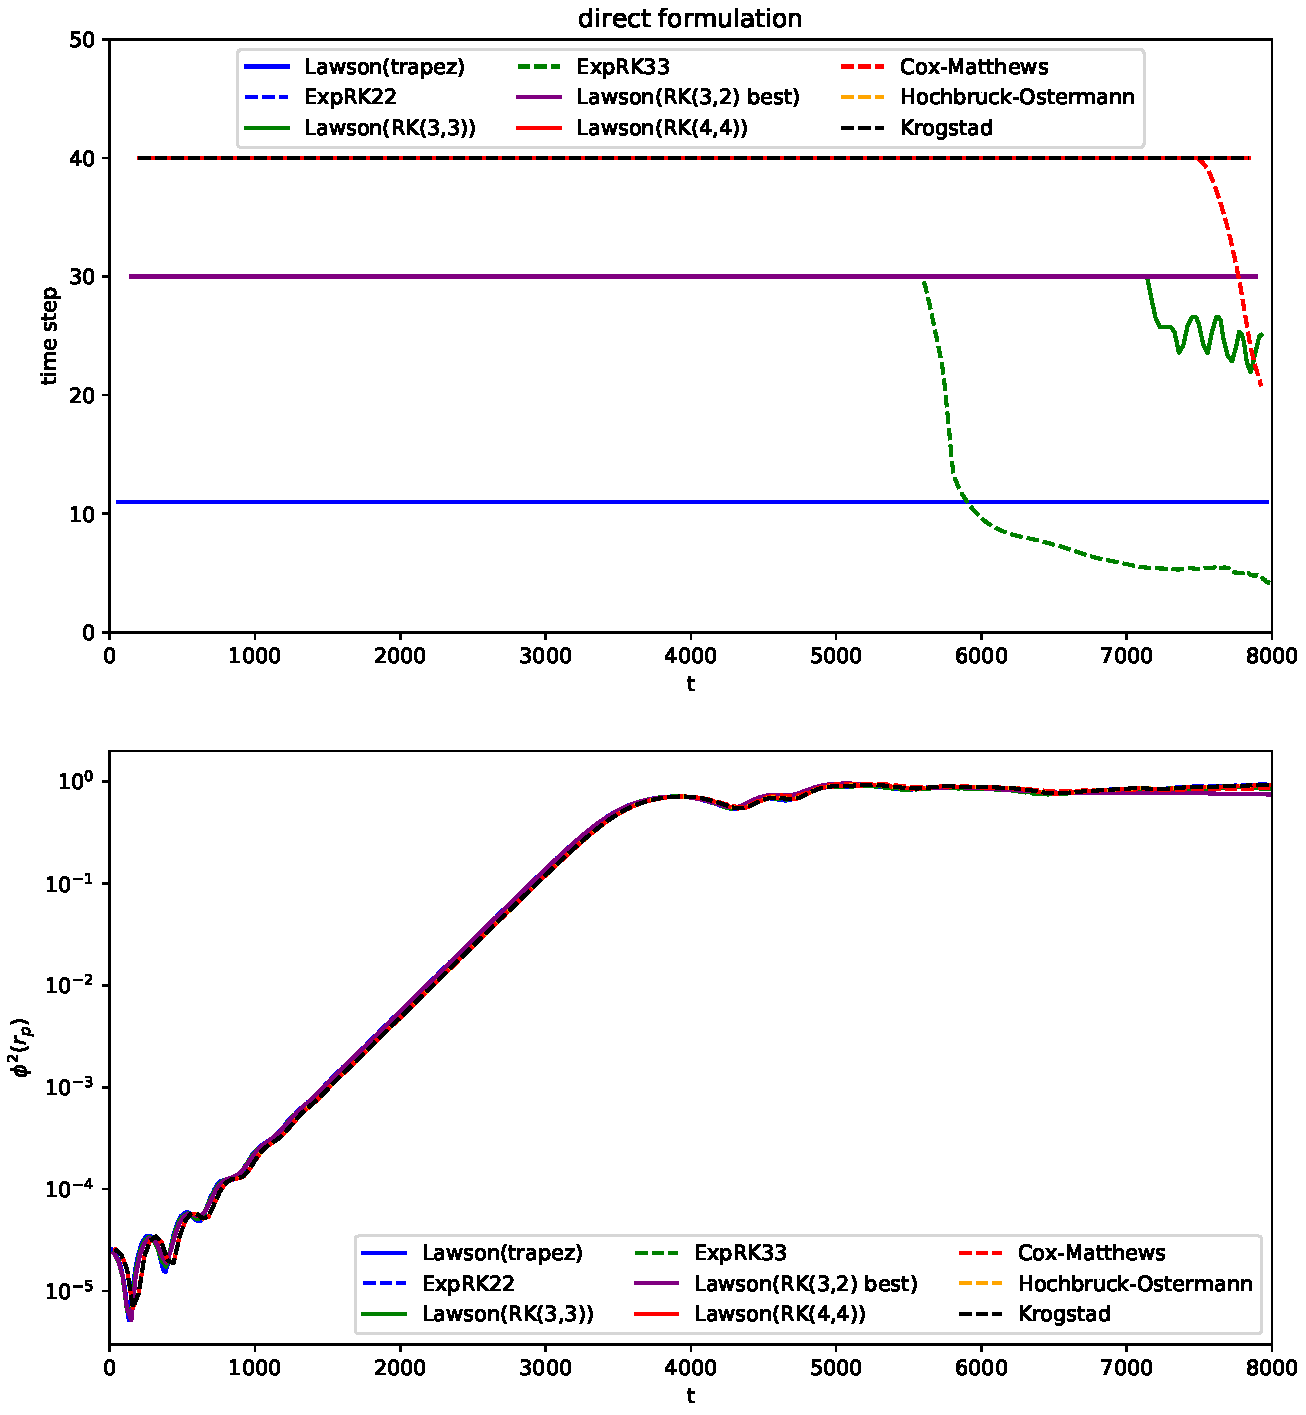
\includegraphics[width=\textwidth]{\localPath/figures/driftkinetic-tol1e-02-32x32x32x64-pert0}%.pdf
	\end{subfigure}
	\begin{subfigure}[b]{0.48\textwidth}
%        \centering 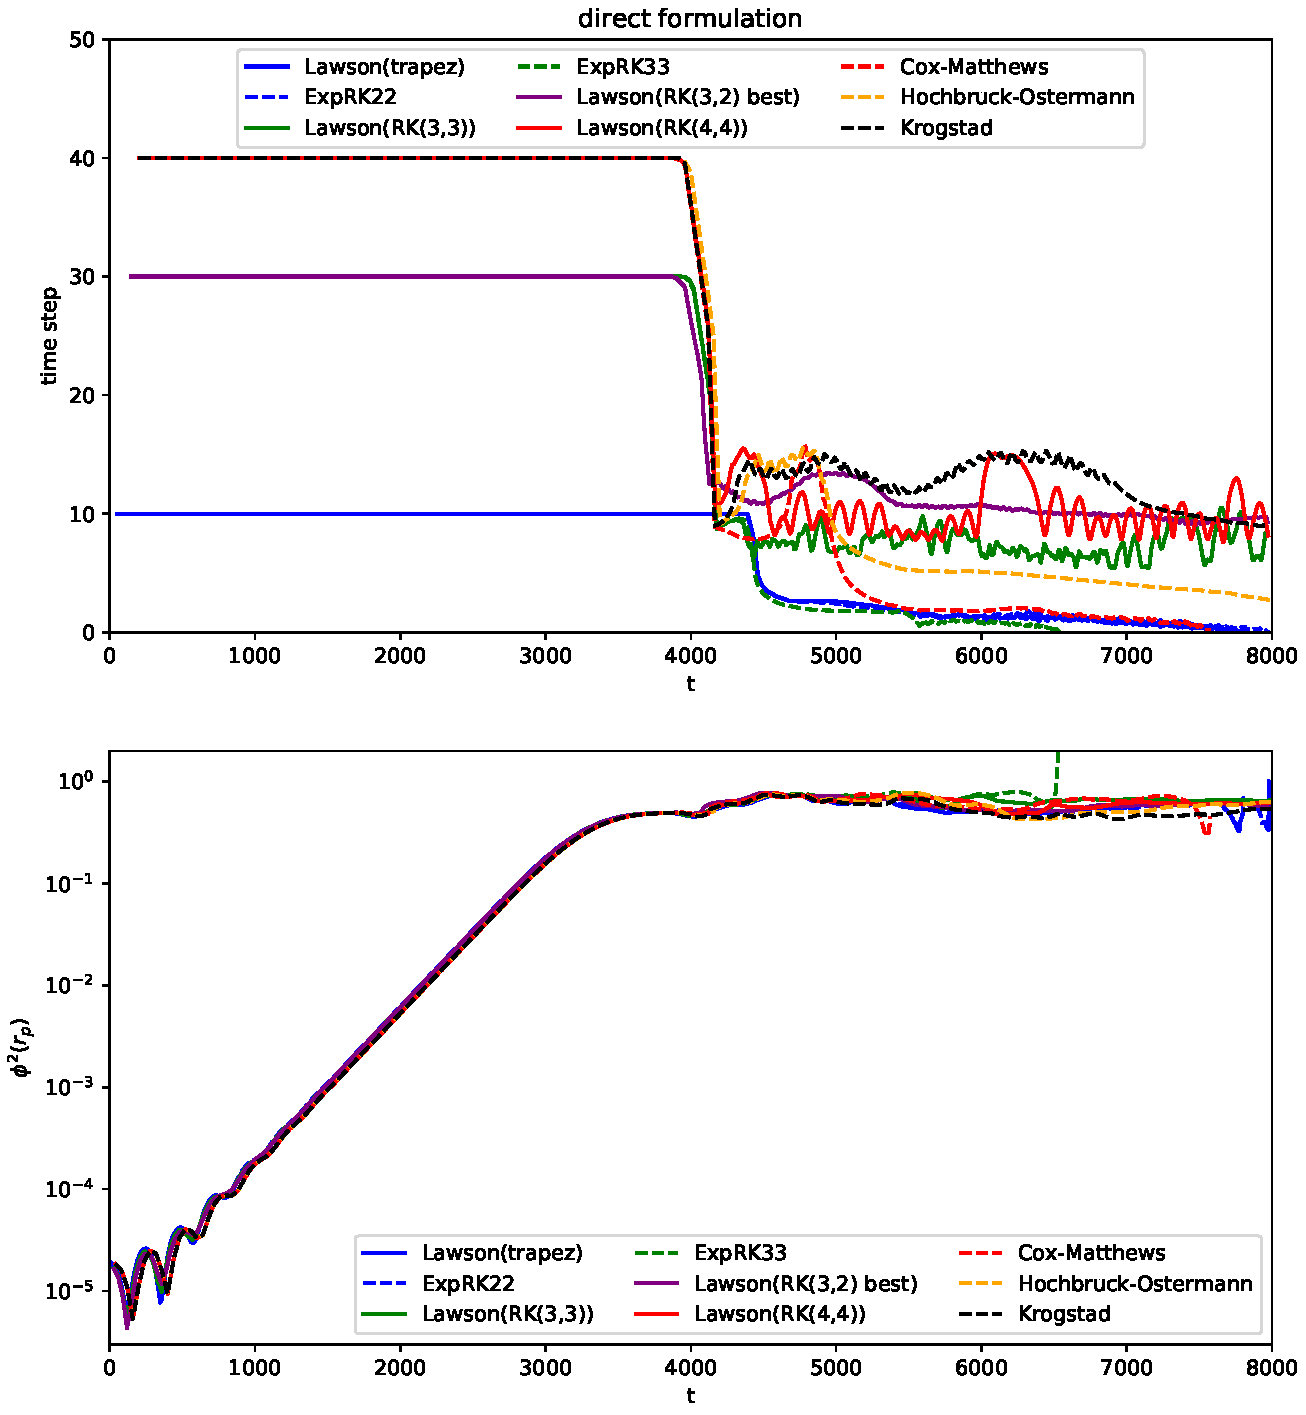
\includegraphics[width=\textwidth]{\localPath/figures/driftkinetic-tol1.00e-02-64x64x64x128-pert0.pdf}
         \centering 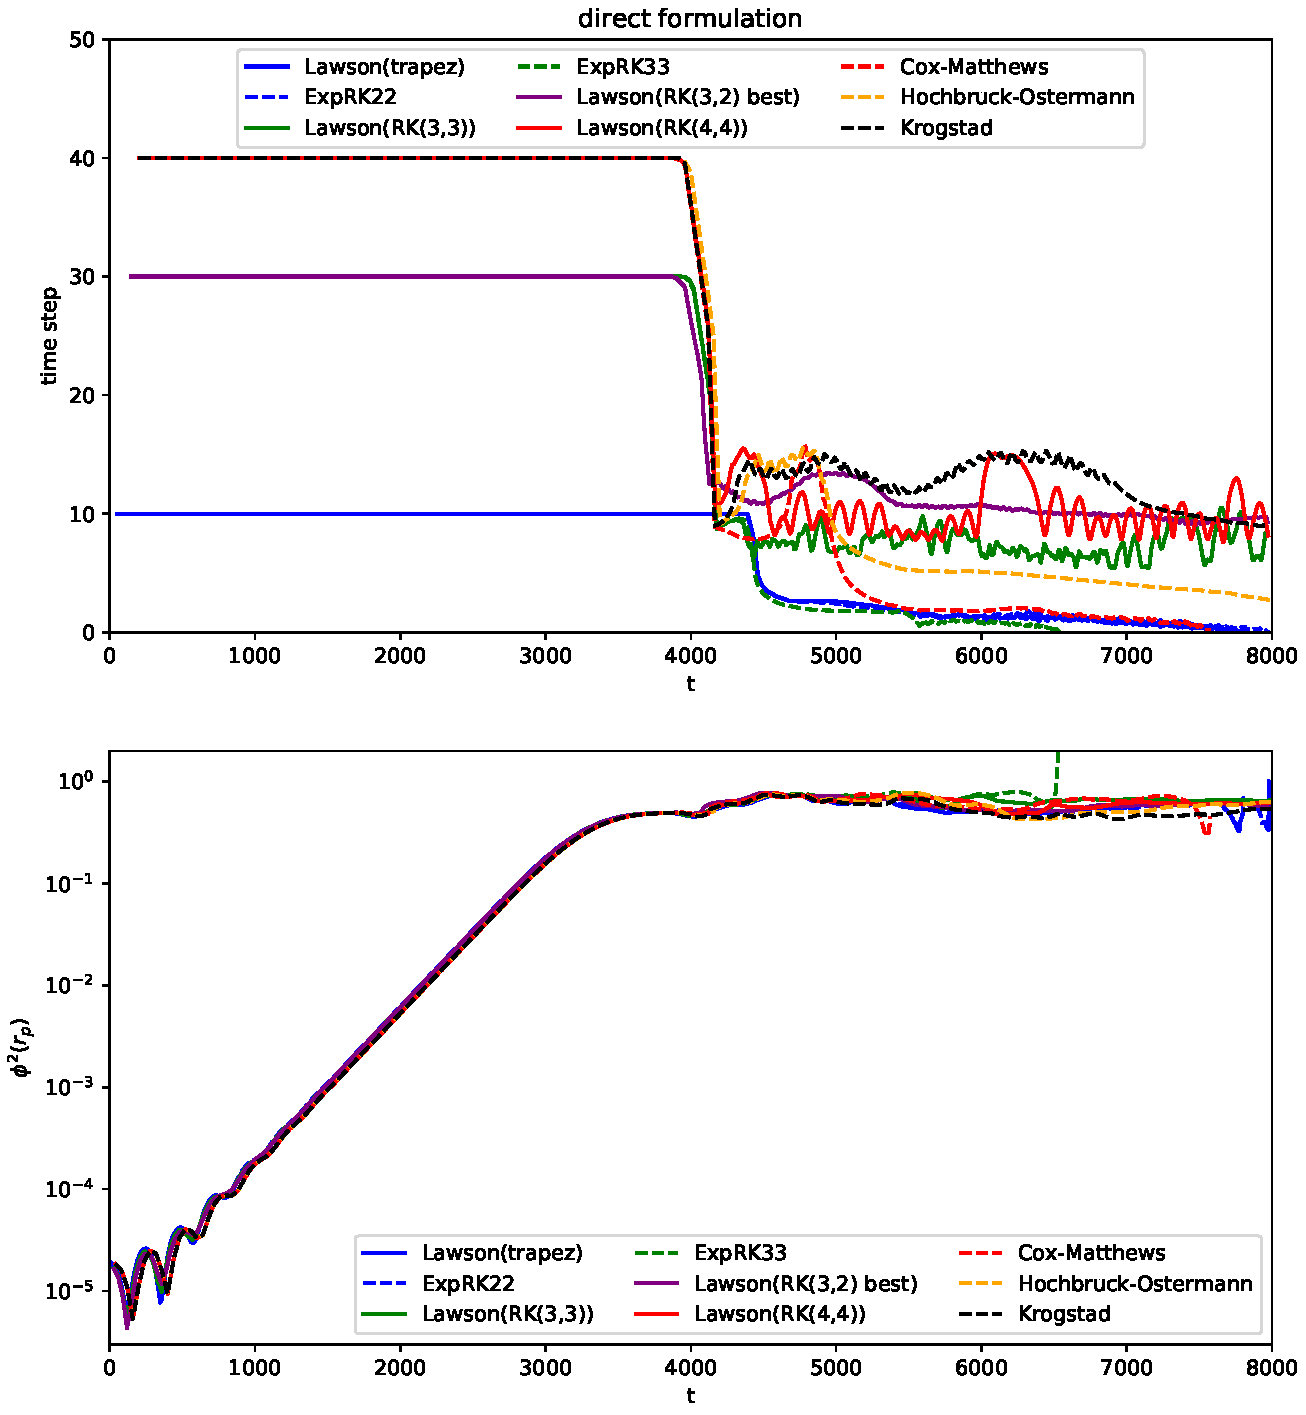
\includegraphics[width=\textwidth]{\localPath/figures/driftkinetic-tol1e-02-64x64x64x128-pert0}%.pdf
	\end{subfigure}
	\caption{Numerical simulation for a number of Lawson methods and exponential integrators for the drift-kinetic model (direct formulation). The upper plots show the time step size as a function of time. The lower plots show the time evolution of the electric energy. The configuration on the left uses $32 \times 32 \times 32 \times 64$ grid points and the configuration on the right uses $64 \times 64 \times 64 \times 128$ grid points.}\label{fig:driftkinetic-pert0}
\end{figure}

In Figure \ref{fig:mass_energy}, the time history of the relative error of the total mass and of the total energy 
are displayed with the phase space discretization $64\times 64\times 64\times 128$ and 
using Lawson($RK(4,4)$) and Cox--Matthews time integrators (the perturbation formulation is used here). Since mass is a linear invariant it is preserved, up to machine precision, by the exponential integrator, see \cite{le2015KP}. We also observe good conservation of energy even in the nonlinear phase, which confirms the excellent behavior of the methods. 

\begin{figure}[h]
	\centering
        \centering 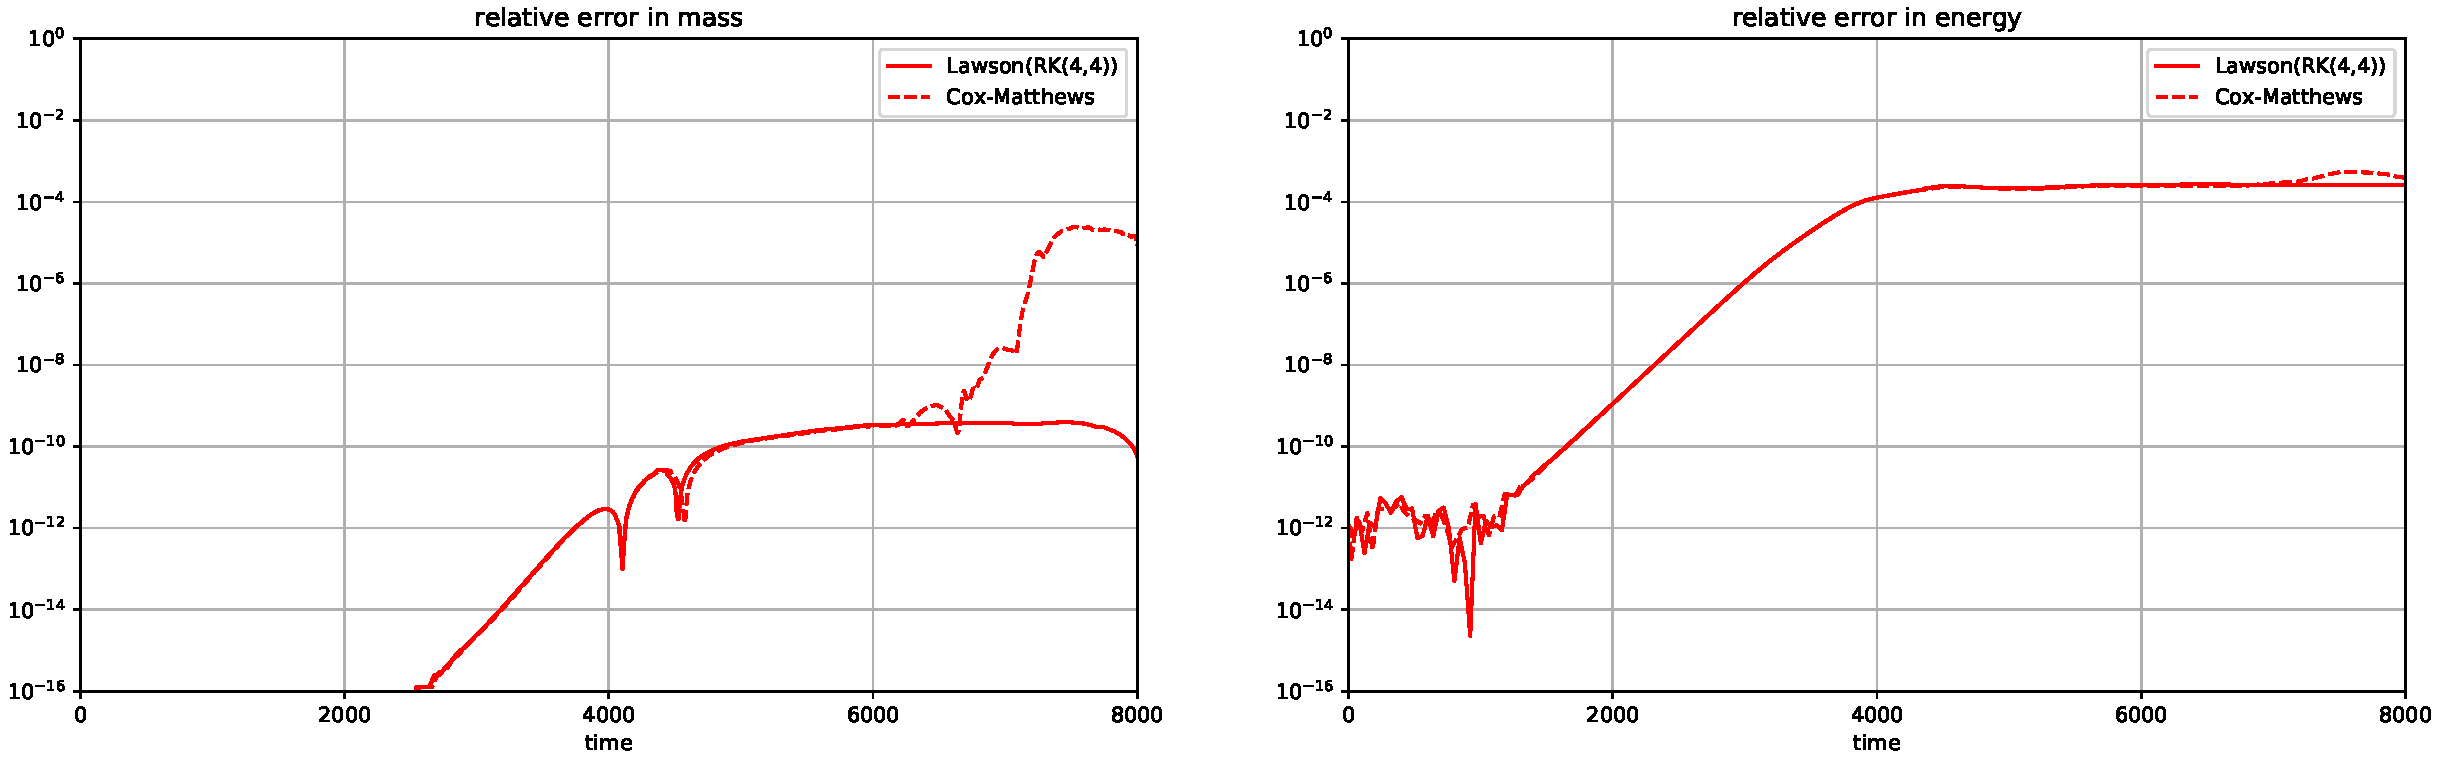
\includegraphics[width=\textwidth]{\localPath/figures/diagnostics.pdf}
    \caption{Numerical simulation for Lawson(RK(4,4)) and the Cox--Matthews method for the drift-kinetic model (perturbation formulation). Left: time history of the error in total mass. 
	Right: time history of the error in total energy. The configuration uses  $64 \times 64 \times 64 \times 128$ grid points.}
	\label{fig:mass_energy}
\end{figure}


Finally, we show slices of the distribution function and the density at different times. The simulation in Figure \ref{fig:snapshots-lrk44} is conducted with the Lawson($RK(4,4)$) scheme and the simulation in Figure \ref{fig:snapshots-cm} with the Cox--Matthews scheme (both 
with the perturbation formulation). In both cases the configuration of Figure \ref{fig:driftkinetic-pert1} and the fine space resolution has been employed. As comparison, a reference solution computed with the Lawson($RK(4,4)$) scheme and a step size controller that keeps the error below $10^{-5}$ per unit time step is shown in Figure \ref{fig:snapshots-ref}. We remark that all simulations show good agreement: the $m=5$ modes in the $\theta$ 
direction are recovered and after initial growth of the unstable mode,
 we can observe a shearing of the structures and the appearance of small scale structures which are typical for the nonlinear phase. 

\begin{figure}[h]
	\centering
    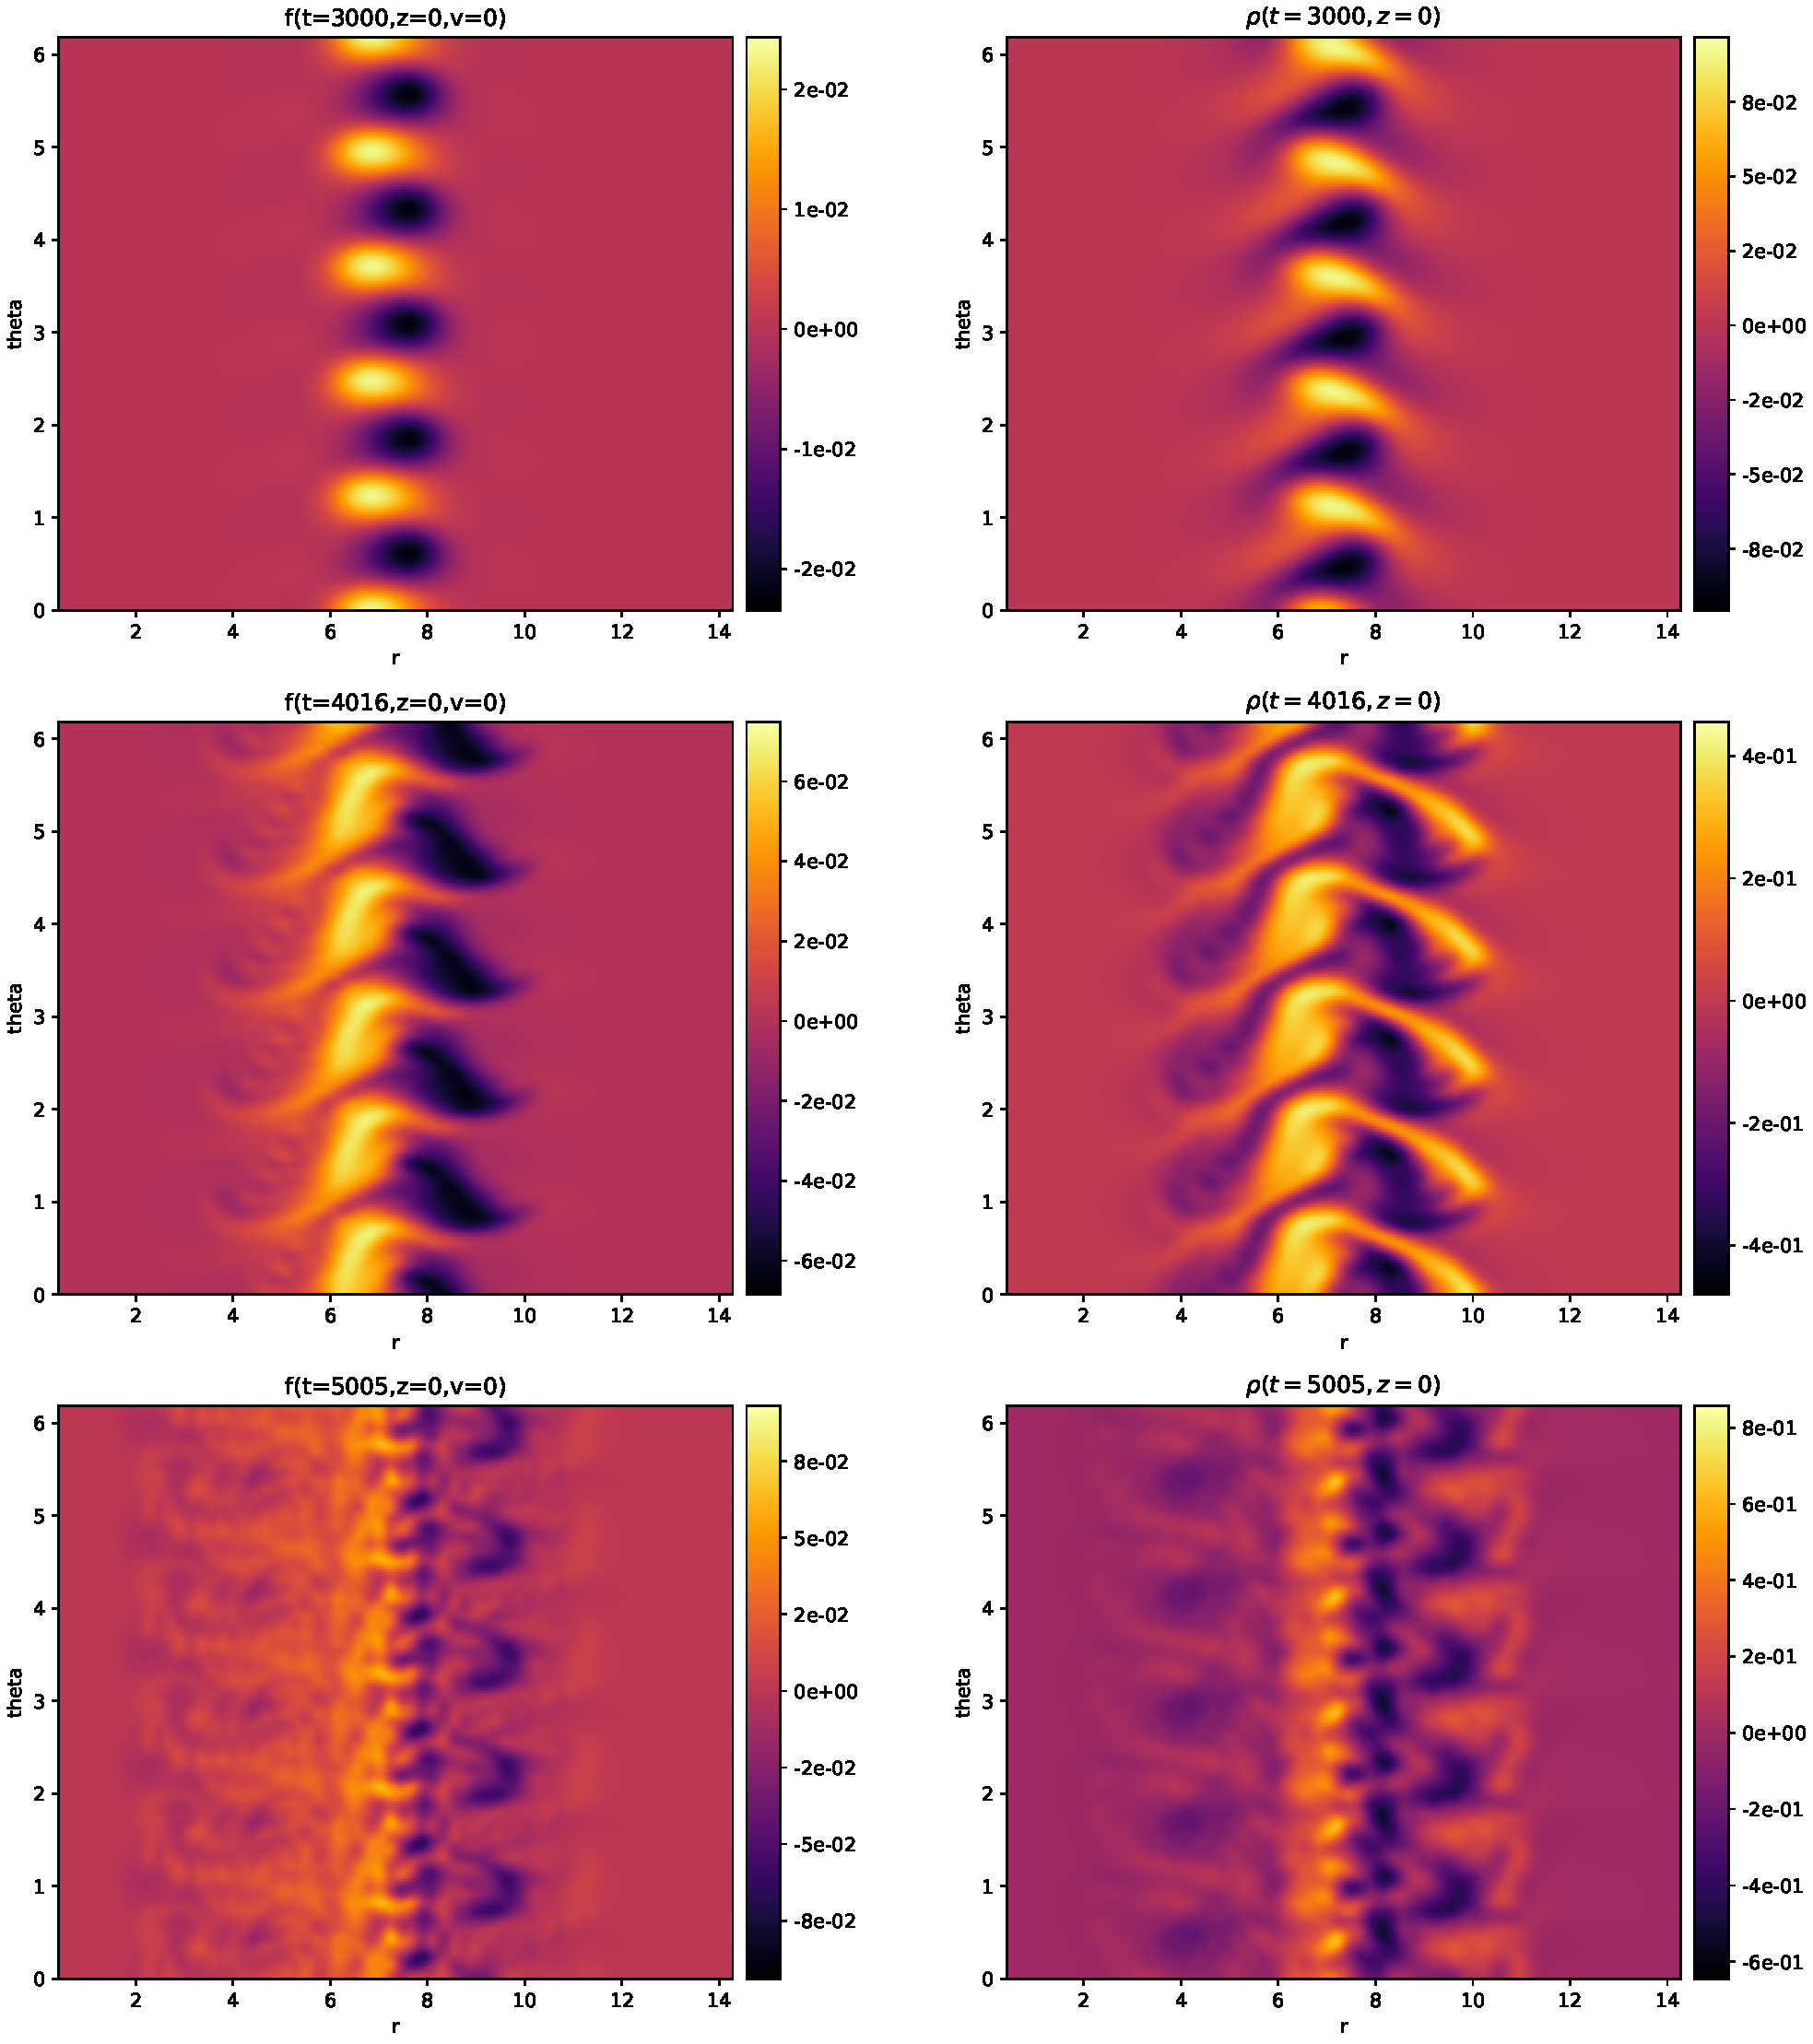
\includegraphics[width=\textwidth]{\localPath/figures/snapshots-lawson-rk44-tol1e-2.pdf}
    \caption{A slices at $(z,v)=(0,0)$ of the distribution function  (on the left) and a slice at $z=0$ of the density (on the right) are shown for times $t=3000$, $4000$, and $5000$. The Lawson($RK(4,4)$) scheme, in the configuration described in section \ref{subsec:driftkinetic-results}, with $64\times64\times64\times128$ grid points is used. \label{fig:snapshots-lrk44}}
\end{figure}


\begin{figure}[h]
	\centering
    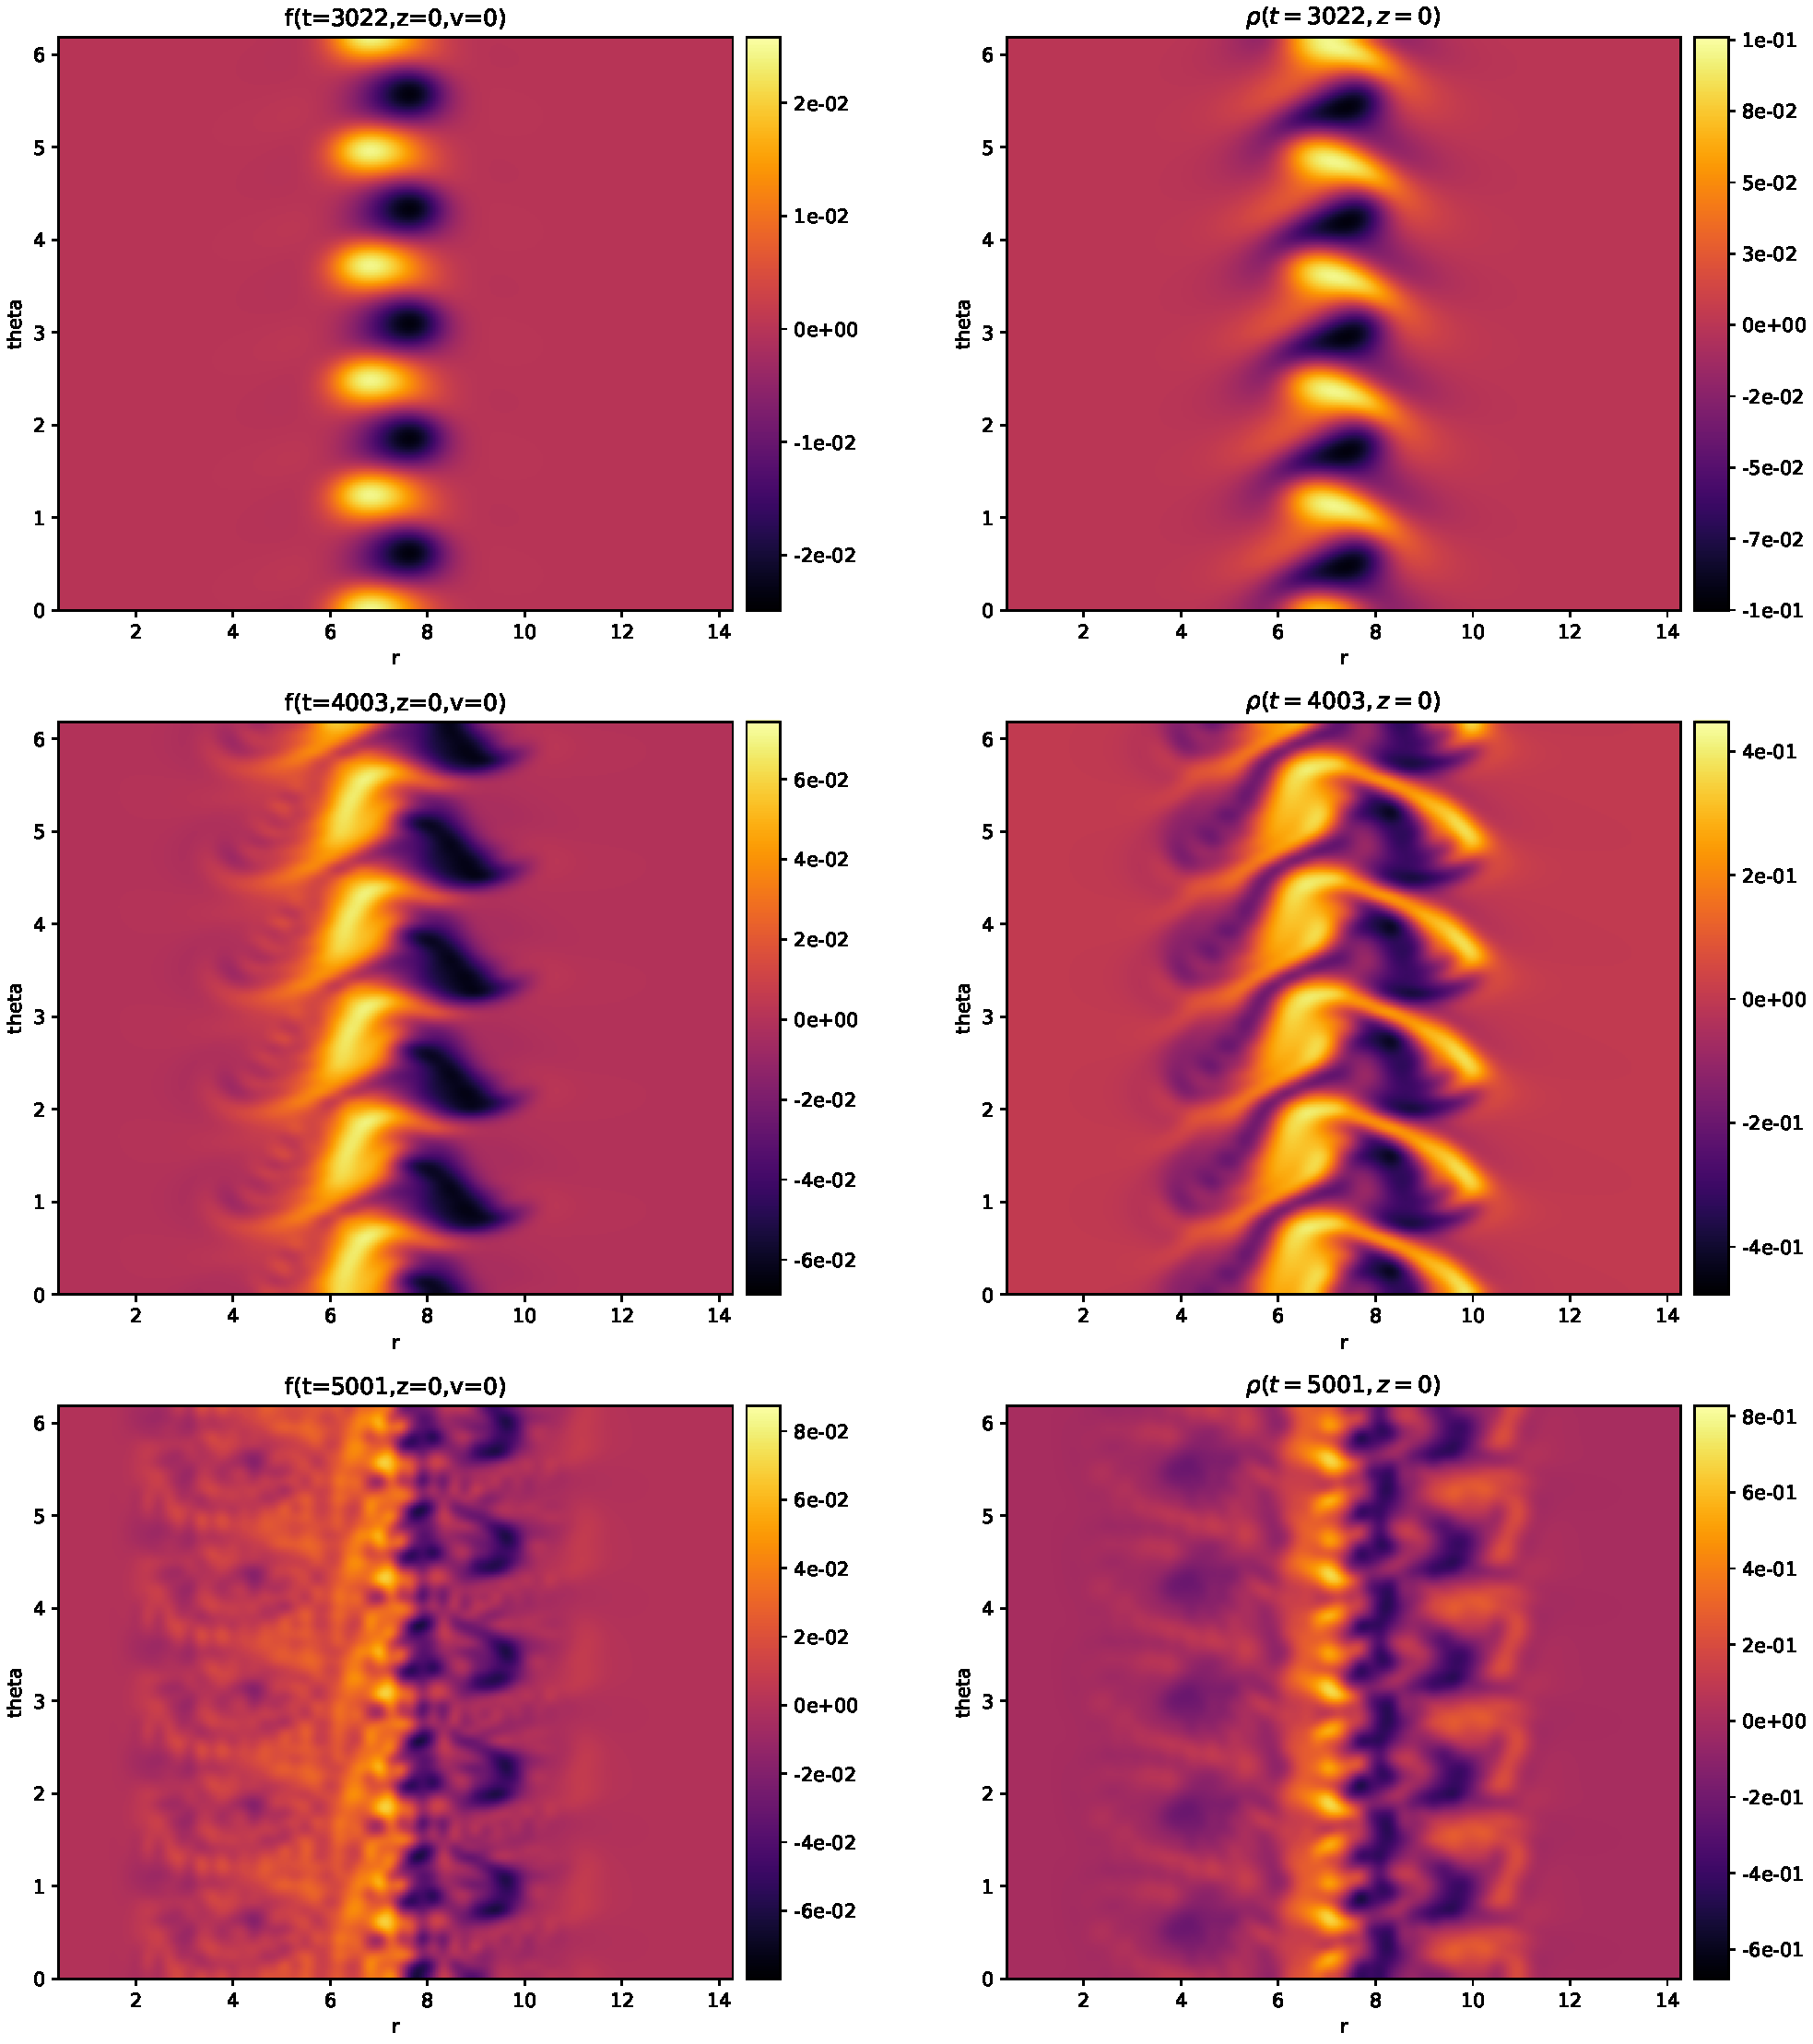
\includegraphics[width=\textwidth]{\localPath/figures/snapshots-coxmatthews-tol1e-2.pdf}
    \caption{A slices at $(z,v)=(0,0)$ of the distribution function  (on the left) and a slice at $z=0$ of the density (on the right) are shown for times $t=3000$, $4000$, and $5000$. The Cox--Matthews scheme, in the configuration described in section \ref{subsec:driftkinetic-results}, with $64\times64\times64\times128$ grid points is used. \label{fig:snapshots-cm}}
\end{figure}


\begin{figure}[h]
	\centering
    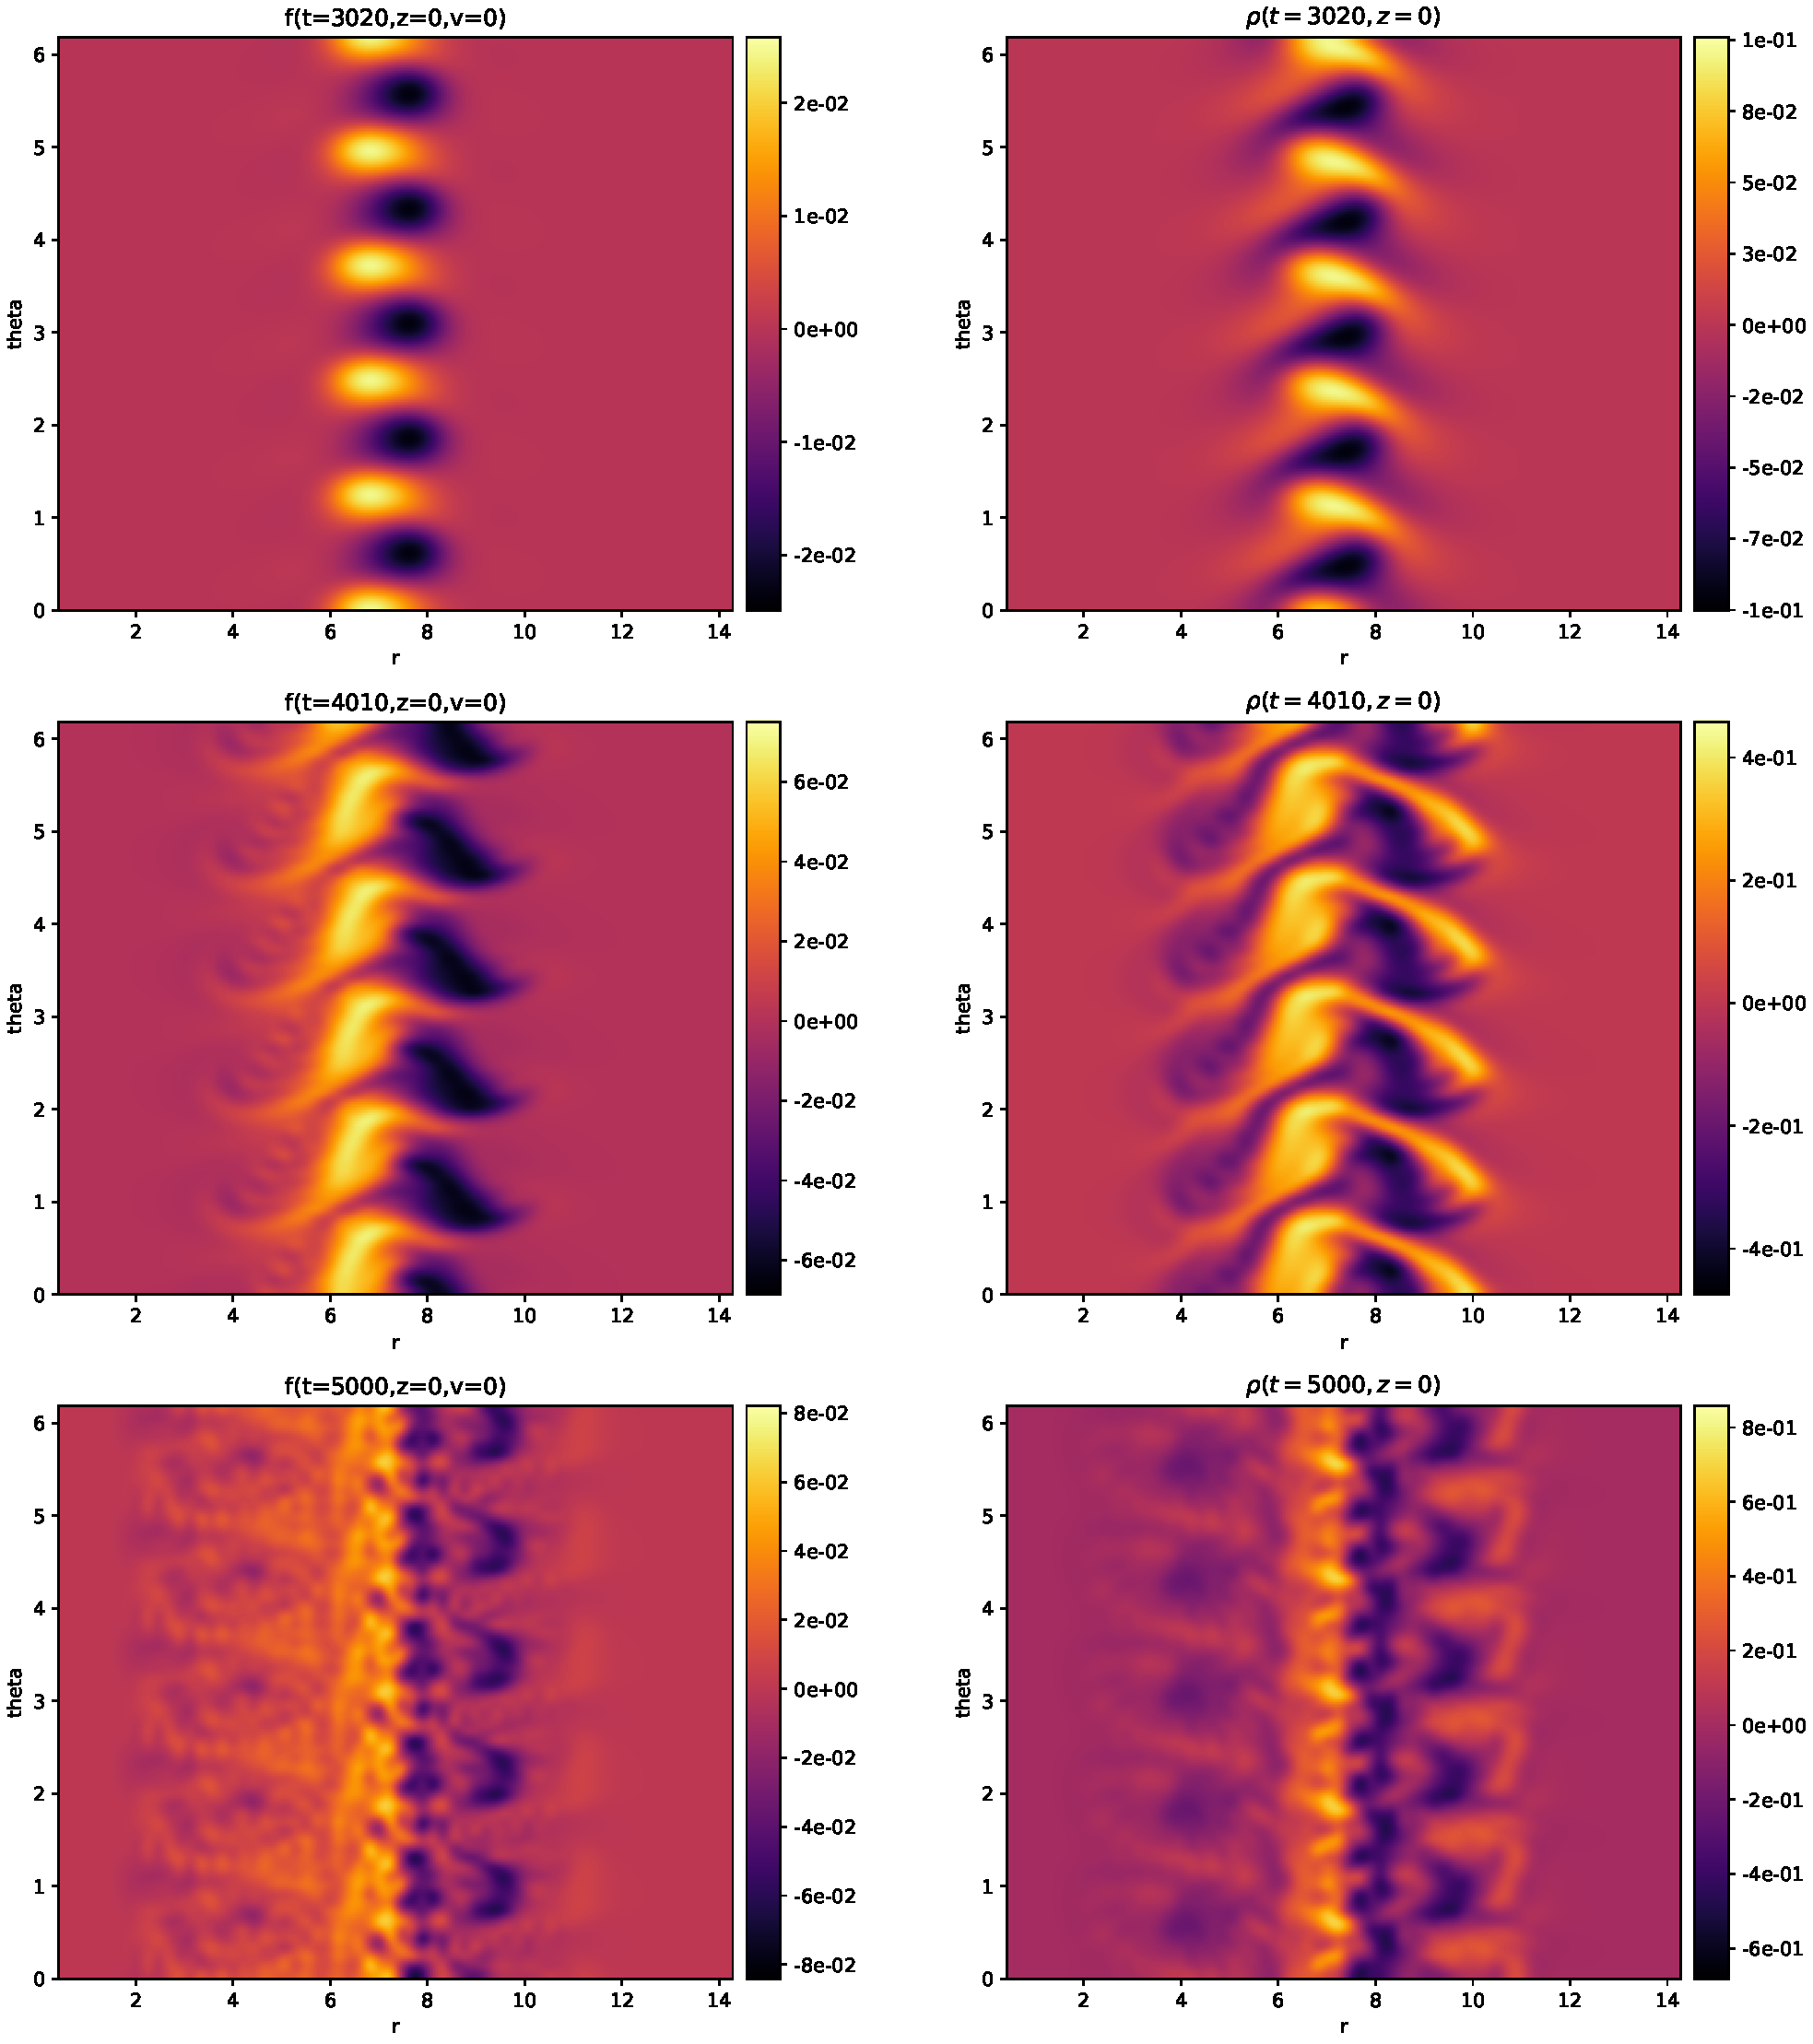
\includegraphics[width=\textwidth]{\localPath/figures/snapshots-reference-1e-5.pdf}
    \caption{A slices at $(z,v)=(0,0)$ of the distribution function  (on the left) and a slice at $z=0$ of the density (on the right) are shown for times $t=3000$, $4000$, and $5000$. The Lawson($RK(4,4)$) scheme with a tolerance of $10^{-5}$ per unit step and $64\times64\times64\times128$ grid points is used. \label{fig:snapshots-ref}}
\end{figure}




\section*{Acknowledgement}
\addcontentsline{toc}{section}{Acknowledgement}

We would like to thank David C. Seal (U.S. Naval Academy) and Sigal Gottlieb (University of Massachusetts, Dartmouth) for the helpful discussion.

This work has been carried out within the framework of the EUROfusion Consortium and has received funding from the Euratom research and training programme 2014- 2018 and 2019-2020 under grant agreement No 633053. The views and opinions expressed herein do not necessarily reflect those of the European Commission. The work has been supported by the French Federation for Magnetic Fusion Studies (FR-FCM) and by the Austrian Science Fund (FWF): project number P 32143-N32. 

\begin{subappendices}
%%%%%%%%%%%%%%%%%%%%%%%%%%%%%%%%%%%%%%%%%%%%%%%%%%%%%%%%%%%%%%%%%%%%%
\section{Butcher tableaus}
\label{butcher}
In this section, we write down the different numerical methods used in this work. As in section \ref{sec:expint},
we consider the following equation
$$
\dot{u} = A u + F(u),
$$
where $A$ is a matrix and $F$ a general nonlinear function of $u$.
The Butcher tableaus for the Lawson integrators used in the main text are stated in this section.
A Lawson method is uniquely determined by the underlying (explicit) Runge--Kutta methods and can be written as follows
$$
\begin{aligned}
        u^{(\ell)} &= e^{c_\ell \Delta t A}u^n + \Delta t\sum_{j=1}^s a_{\ell, j} e^{-(c_j-c_\ell)\Delta t A} F(u^{(j)}),  \\
    u^{n+1} &= e^{\Delta t A}u^n + \Delta t\sum_{j=1}^s    b_j e^{(1-c_j)\Delta t A} F(u^{(j)}),
  \end{aligned}
$$
where the coefficients  $a_{\ell, j}$ and $b_j$ are given by the Butcher tableaus.
The Butcher tableaus for the \textit{RK(2,2) best}, \textit{RK(3,3)} (the classic method of order 3),
and \textit{RK(4,4)} (the classic method of order 4) are shown in Table \ref{rks}.

\begin{table}[h]
\centering
\begin{tabular}
{c|cccc}
$0$\\
$\frac{1}{2}$ & $\frac{1}{2}$\\
$\frac{1}{2}$ &$0$ &$\frac{1}{2}$ \\
$1$& $0$& $0$& $1$\\
\hline
& $\frac{1}{6}$ &$\frac{1}{3}$ &$\frac{1}{3}$ &$\frac{1}{6} $
\end{tabular}
\hspace{1cm}
\begin{tabular}
{c|ccc}
$0$\\
$\frac{1}{2}$ & $\frac{1}{2}$\\
$1 $ &$-1$ &$2$ \\
\hline
& $\frac{1}{6}$ &$\frac{2}{3}$ &$\frac{1}{6}$
\end{tabular}
\hspace{1cm}
\begin{tabular}
{c|ccc}
$0$\\
$\frac{1}{2}$ & $\frac{1}{2}$\\
$\frac{1}{2}$              &$0$ &$\frac{1}{2}$ \\
\hline
& $0$ &$0$ &$1$
\end{tabular}
    \caption{Butcher tableaus for $RK(4,4)$ (left), $RK(3,3)$ (middle) and $RK(3,2)\text{ best}$ (right).}
\label{rks}
\end{table}


A general exponential integrator can be written as
$$
  \begin{aligned}
        u^{(\ell)} &= u^n + \Delta t\sum_{j=1}^s a_{\ell, j}(\Delta t A)\left( F(u^{(j)}) + A u^n \right) \\
    u^{n+1} &= u^n + \Delta t\sum_{j=1}^s    b_j(\Delta t A)\left( F(u^{(j)}) + A u^n \right),
  \end{aligned}
$$
where the coefficients $a_{\ell, j}(\Delta t A)$ and $b_j(\Delta t A)$ can be written as a linear combination of $\varphi_\ell$ and $\varphi_{\ell,  j}$
(see \cite{ei})
$$
 \varphi_\ell(z) = \frac{e^{z} - \sum_{k=0}^{\ell-1}\frac{1}{k!}z^k}{z^\ell},
$$
and we use the notations $\varphi_\ell :=\varphi_\ell(\Delta t A)$ and $\varphi_{\ell,j} := \varphi_\ell(c_j \Delta t A)$. The coefficients are collected in tableau form, see Table \ref{tab:butcher_expRK}.
\begin{table}[h]
  \centering
  \begin{tabular}{c|ccccc}
    $0$    &  & $$ & $$  & \\
    $c_2$    & $a_{2, 1}$ &  & $$ &  \\
    $\vdots$ & $\vdots$ & $\ddots$ & $$ &  \\
    $c_s$    & $a_{s1}$ & $\cdots$ & $a_{s, s-1}$ &  \\ \hline
    & $b_1$ & $\cdots$ & $b_{s-1}$ & $b_s$
  \end{tabular}
    \caption{Butcher tableau of a general exponential integrators}\label{tab:butcher_expRK}
\end{table}
The Butcher tableaus for the exponential integrators used in the main text are given in Tables \ref{butcherexprk22}, \ref{butcherK}, \ref{butcherHO} and \ref{butcherCM}.

\begin{table}[H]
  \centering
  \begin{tabular}{c|cc}
    $0$ & \\
    $1$ & $\varphi_{1,2}$ \\
    \hline
    & $\varphi_1 - \varphi_2$ & $\varphi_2$
  \end{tabular}
  \caption{Butcher tableau of ExpRK22.}
  \label{butcherexprk22}
\end{table}

\begin{table}[H]
  \centering
  \begin{tabular}{c|cccc}
    $0$           & \\
    $\frac{1}{2}$ & $\frac{1}{2}\varphi_{1,2}$ \\
    $\frac{1}{2}$ & $\frac{1}{2}\varphi_{1,3}-\varphi_{2,3}$ & $\varphi_{2,3}$ \\
    $1$           & $\varphi_{1,4}-2\varphi_{2,4}$           & $0$          & $2\varphi_{2,4}$ \\
    \hline
    & $\varphi_1-3\varphi_2+4\varphi_3$ & $2\varphi_2-4\varphi_3$ & $2\varphi_2-4\varphi_3$ & $-\varphi_2+4\varphi_3$ \\
  \end{tabular}
  \caption{Butcher tableau of the Krogstad method.}
    \label{butcherK}
\end{table}

\begin{table}[H]
  \centering
  \begin{tabular}{c|ccccc}
    $0$           & \\
    $\frac{1}{2}$ & $\frac{1}{2}\varphi_{1,2}$ \\
    $\frac{1}{2}$ & $\frac{1}{2}\varphi_{1,3}-\varphi_{2,3}$    & $\varphi_{2,3}$ \\
    $1$           & $\varphi_{1,4}-2\varphi_{2,4}$              & $\varphi_{2,4}$ & $\varphi_{2,4}$ \\
    $\frac{1}{2}$ & $\frac{1}{2}\varphi_{1,5}-2a_{5,2}-a_{5,4}$ & $a_{5,2}$       & $a_{5,2}$       & $\frac{1}{4}\varphi_{2,5} - a_{5,2}$ \\
    \hline
    & $\varphi_1-3\varphi_2+4\varphi_3$ & $0$ & $0$ & $-\varphi_2+4\varphi_3$ & $2\varphi_2-8\varphi_3$ \\
  \end{tabular}

    $$\begin{aligned} a_{5,2} &= \frac{1}{2}\varphi_{2,5}-\varphi_{3,4}+\frac{1}{4}\varphi_{2,4}-\frac{1}{2}\varphi_{3,5} \\ a_{5,4} &= \frac{1}{4}\varphi_{2,5}-a_{5,2} \end{aligned}
  $$
  \caption{Butcher tableau of the Hochbruck--Ostermann method.}
  \label{butcherHO}
\end{table}

\begin{table}[H]
  \centering
  \begin{tabular}{c|cccc}
    $0$           & \\
    $\frac{1}{2}$ & $\frac{1}{2}\varphi_{1,2}$ \\
    $\frac{1}{2}$ & $0$                        & $\frac{1}{2}\varphi_{1,3}$ \\
    $1$           & $\frac{1}{2}\varphi_{1,3}(\varphi_{0,3}-1)$ & $0$ & $\varphi_{1,3}$ \\
    \hline
    & $\varphi_1-3\varphi_2+4\phi_3$ & $2\varphi_2-4\varphi_3$ & $2\varphi_2-4\varphi_3$ & $4\varphi_3-\varphi_2$ \\
  \end{tabular}
  \caption{Butcher tableau of the Cox--Matthews method.}
    \label{butcherCM}
\end{table}


\section{WENO5 scheme}
\label{app_weno}
The different ingredients of the WENO5 scheme used in \eqref{vp_weno} are detailed here. First the fluxes are given by
$$
  \begin{aligned}
    {f}_{j+\frac{1}{2}}^+   =\ & w_0^+\left(  \frac{2}{6}f_{j-2} - \frac{7}{6}f_{j-1} + \frac{11}{6}f_{j}   \right)
                                +    w_1^+\left( -\frac{1}{6}f_{j-1} + \frac{5}{6}f_{j}   +  \frac{2}{6}f_{j+1} \right) \\
                                +  & w_2^+\left(  \frac{2}{6}f_{j}   + \frac{5}{6}f_{j+1} -  \frac{1}{6}f_{j+2} \right)
  \end{aligned}
$$
and
$$
  \begin{aligned}
    {f}_{j+\frac{1}{2}}^-   =\ & w_2^-\left( -\frac{1}{6}f_{j-1} + \frac{5}{6}f_{j}   + \frac{2}{6}f_{j+1} \right)
                                +    w_1^-\left(  \frac{2}{6}f_{j}   + \frac{5}{6}f_{j+1} - \frac{1}{6}f_{j+2} \right) \\
                                +  & w_0^-\left( \frac{11}{6}f_{j+1} - \frac{7}{6}f_{j+2} + \frac{2}{6}f_{j+3} \right).
  \end{aligned}
$$
The weights are defined through the $\beta$ coefficients
$$
  \begin{aligned}
    \beta_0^+ &= \frac{13}{12}(\underbrace{f^+_{j-2} - 2f^+_{j-1} + f^+_{j}  }_{\Delta x^2(f''_j + \mathcal{O}(\Delta x))}))^2 + \frac{1}{4}( \underbrace{f^+_{j-2} - 4f^+_{j-1} + 3f^+_{j}}_{2\Delta  f'_j + \mathcal{O}(\Delta x^2))}  )^2 \\
    \beta_1^+ &= \frac{13}{12}( \underbrace{f^+_{j-1} - 2f^+_{j}   + f^+_{j+1}}_{\Delta x^2(f''_j + \mathcal{O}(\Delta x^2))} )^2 + \frac{1}{4}( \underbrace{f^+_{j-1} -  f^+_{j+1}}_{2\Delta x f'_j + \mathcal{O}(\Delta x^2))})^2 \\
    \beta_2^+ &= \frac{13}{12}( \underbrace{f^+_{j}   - 2f^+_{j+1} + f^+_{j+2}}_{\Delta x^2(f''_j + \mathcal{O}(\Delta x))} )^2 + \frac{1}{4}(\underbrace{3f^+_{j}   - 4f^+_{j+1} +  f^+_{j+2}}_{-2\Delta  f'_j + \mathcal{O}(\Delta x^2))})^2 \\
  \end{aligned}
$$
with
$$
  \begin{aligned}
    \beta_0^- &= \frac{13}{12}(f^-_{j+1} - 2f^-_{j+2} + f^-_{j+3})^2 + \frac{1}{4}(3f^-_{j+1} - 4f^-_{j+2} +  f^-_{j+3})^2 \\
    \beta_1^- &= \frac{13}{12}(f^-_{j}   - 2f^-_{j+1} + f^-_{j+2})^2 + \frac{1}{4}( f^-_{j}   -  f^-_{j+2})^2 \\
    \beta_2^- &= \frac{13}{12}(f^-_{j-1} - 2f^-_{j}   + f^-_{j+1})^2 + \frac{1}{4}( f^-_{j-1} - 4f^-_{j}   + 3f^-_{j+1})^2 \\
  \end{aligned}
$$
Then, the normalized weights are
$$
  \alpha_i^\pm = \frac{\gamma_i}{(\varepsilon + \beta_i^\pm)^2},\quad i=0,1,2,
$$
where  $\varepsilon$ is a numerical regularization parameter set to $10^{-6}$
and $\gamma_0=\frac{1}{10}$, $\gamma_1=\frac{6}{10}$
and $\gamma_2=\frac{3}{10}$. Finally the weights are given by
$$
  w_i^\pm = \frac{\alpha_i^\pm}{\sum_m \alpha_m^\pm},\quad i=0,1,2.
$$
\end{subappendices}


\end{otherlanguage}
%\selectlanguage{french}




\clearemptydoublepage
% !TEX root = ../main.tex
\renewcommand{\localPath}{chap2}

\chapter{Modèle hybride linéarisé dans~le~cas~$1dx-1dv$}
\label{chap2}

Ce chapitre est la première partie de l'étude du modèle hybride linéarisé~\eqref{eq:0:vmhl:1}-\eqref{eq:0:vmhl:4} dans le cadre restreint $1dx-1dv$. Cela permet de mettre en place certains outils d'analyse, et d'utiliser les résultats du chapitre précédent dans le contexte d'un modèle hybride linéarisé. Ce travail collaboratif avec Anaïs Crestetto\footnote{Université de Nantes, Laboratoire de Mathématiques Jean Leray}, Nicolas Crouseilles\footnote{Univ Rennes, Inria Bretagne Atlantique (MINGuS) \& ENS Rennes} et Yingzhe Li\footnote{Max Planck Institute, Institut Für Plasmaphysik, Germany} a mené à un article \emph{Comparison of high-order Eulerian methods for electron hybrid model} soumis dans \emph{Journal of Computational Physics} en 2021.

%% section 1
% !TEX root = ../chap3.tex

\section{Introduction}

L'objectif de ce chapitre est d'étendre les stratégies développées pour la résolution d'un modèle hybride linéarisé, présentées dans le chapitre~\ref{chap2}, au cas $1dz-3dv$ permettant de prendre en compte, entre autre, les effets du champ magnétique sur la dynamtique des particules. Nous étudierons dans ce chapitre un modèle hybride, ce qui suppose que la distribution de particules est composée de deux populations, une première ayant une vitesse thermique faible, et considérée comme \emph{froide}, dont on approximera la dynamique comme celle d'un fluide ; une seconde population ayant une vitesse thermique plus élevée, considérée comme \emph{chaude}, mais contrairement au chapitre~\ref{chap2}, celle-ci n'a pas besoin d'être distribuée selon une bi-maxwellienne. Ce type de modèle peut être utilisé pour modéliser des particules d'un plasma dans un tokamak, ou des particules du vent solaire interagissant avec la magnétosphère terrestre. Dans ces contextes les particules se déplacent de manière hélicoïdale selon les lignes du champ extérieur $\vb{B}_0 = (0,0,B_0)^\top$, et seul le déplacement dans cette direction sera étudié ici, ce qui explique le nom de la seule variable d'espace considérée : $z$. Pour le déplacement hélicoïdale complet \Josselin{il faudrait ajouter ici une référence que je n'ai pas car je ne connais pas trop ces modèles, de mémoire c'est ce que faisait Xiaofei}.

La prise en compte des effets du champ magnétique dans le modèle nous mène à considérer un système à 7 inconnues $(j_{c,x},j_{c,y},B_x,B_y,E_x,E_y,f_h)$, ce qui induit un coût de calcul bien plus important avec les méthodes eulériennes que nous étudions. Pour diminuer ce coût de calcul nous souhaitons diminuer le nombre d'itérations tout en assurant la stabilité des méthodes considérées ; cela se fait en augmentant le pas de temps $\Delta t$ et en estimant les contraintes de stabilité. L'utilisation de méthodes d'ordre élevés en temps, en espace et en vitesse, permet de réduire l'erreur, capturer la dynamique non-linéaire du système, avec peu de points de discrétisation.

Nous souhaitons dans ce chapitre comparer deux méthodes d'ordre élevé en temps et dans l'espace des phrases, sur un cas à 4 dimensions, plus proches d'applications physiques, il s'agit d'une généralisation des deux stratégies développées dans le chapitre~\ref{chap2}, une méthode de \emph{splitting} et une méthode de Lawson. La contrainte du nombre de dimensions ne permet pas de raffiner le maillage\footnote{Pour une discrétisation de $128$ points par direction, la grille contient $128^4$ points, soit, représentées avec des réels à virgule flottante à double précision (64 bits), un espace mémoire de 2Go pour la seule variable $f_h$ ; une méthode de Lawson d'ordre 4 nécessite la sauvegarde des étages intermédiaires, donc $4\times 2\textrm{Go}$ minimum. L'utilisation de transformées de Fourier impose de travailler avec des nombres complexes, ce qui nécessite de doubler l'utilisation mémoire pour la même précision.}, ce qui ne permet pas l'accès à une solution de référence, nous devrons nous contenter de regarder les invariants (comme l'énergie totale), et de comparer les résultats aux taux d'instabilités fournis par les relations de dispersion.

Pour résoudre les problèmes que pose ce problème nous présenterons tout d'abord le modèle hybride $1dz-3dv$, puis nous détaillerons les schémas numériques que nous considérons. La méthode de \emph{splitting} hamiltonien contient 7 étapes, rendant de fait l'ordre élevé (méthode de Suzuki) trop coûteux pour approfondir son étude, nous nous concentrerons donc sur des méthodes de \emph{splitting} d'ordre plus faible. Pour la méthode de Lawson, il est envisageable d'effectuer un filtrage du terme induit pas le champ magnétique externe $\vb{B}_0$, permettant d'augmenter le pas de temps stabilisant la méthode. La partie linéaire du système introduit une matrice dont il n'est pas possible de calculer exactement son exponentielle, pourtant nécessaire pour la mise en œuvre d'une méthode de Lawson perforante. Nous étudierons un premier cas où nous ne profitons pas pleinement de toute la partie linéaire du système, introduisant ainsi une condition de stabilité ; puis nous proposerons une méthode permettant, à l'aide de méthodes approchées comme la troncature de la série de Taylor ou les approximants de Padé, de calculer une approximation de l'exponentielle de toute la partie linéaire, permettant ainsi de se soustraire à une condition de stabilité. \Josselin{Mettre les références vers les sections.}

%% section 2
% !TEX root = ../chap3.tex

\section{Présentation du modèle}

\begin{align}
  \label{eq:VHM:jx}
  &\pdv{j_{c,x}}{t} = \Omega_{pe}^2 { E}_x - { j}_{c,y}B_0,\\
  \label{eq:VHM:jy}
  &\pdv{j_{c,y}}{t} = \Omega_{pe}^2 { E}_y + { j}_{c,x}B_0,\\
  \label{eq:VHM:Bx}
  &\pdv{B_{x  }}{t} = \partial_z E_y,\\
  \label{eq:VHM:By}
  &\pdv{B_{y  }}{t} = -\partial_z E_x,\\
  \label{eq:VHM:Ex}
  &\pdv{E_{x  }}{t} =-\partial_z B_y - {j}_{c,x} + \int v_x f_h \dd{\vb{v}},\\
  \label{eq:VHM:Ey}
  &\pdv{E_{y  }}{t} =\partial_z B_x - {j}_{c,y} + \int v_y f_h \dd{\vb{v}}, \\
  \label{eq:VHM:fh}
  &\pdv{f_{h  }}{t} +  v_z\partial_z f_h - \left(E_x + v_y B_0 - v_zB_y\right)\partial_{v_x} f_h\\
  &\hspace{2cm}- \left(E_y - v_x B_0 + v_z B_x\right)\partial_{v_y} f_h- \left(v_x B_y- v_y B_x\right)\partial_{v_z} f_h = 0.\nonumber
\end{align}
Cela nous permet de définir l'hamiltonien :
\begin{equation}
  \mathcal{H} = {}
      \underbrace{\frac{1}{2}\int_{\mathbb{R}}(E_x^2+E_y^2) \dd{z}}_{\mathcal{H}_E}
    + \underbrace{\frac{1}{2}\int_{\mathbb{R}}(B_x^2+B_y^2) \dd{z}}_{\mathcal{H}_B}
    + \underbrace{\frac{1}{2}\int_{\mathbb{R}}\frac{1}{\Omega_{pe}^2}(j_{c,x}^2+j_{c,y}^2) \dd{z}}_{\mathcal{H}_{j_c}}
    + \underbrace{\frac{1}{2}\int_{\mathbb{R}}\int_{\mathbb{R}^2}|\vb{v}|^2 f_h \dd{\vb{v}}\dd{z}}_{\mathcal{H}_{f_h}}
  \label{eq:ham1dz3dv}
\end{equation}

On définit le crouchet suivant, définit pour deux fonctionnelles $\mathcal{F}$ et $\mathcal{G}$ :
\begin{equation}
  \begin{aligned}
    \{ \mathcal{F},\mathcal{G} \}[ j_{c,x}, j_{c,y}, B_x, B_y, E_x, E_y, f_h] &=
                       \int_{\mathbb{R}}\int_{\mathbb{R}^3} f_h \left( \partial_z\fdv{\mathcal{F}}{f_h}\partial_{v_z}\fdv{\mathcal{G}}{f_h} - \partial_{v_z}\fdv{\mathcal{F}}{f_h}\partial_z\fdv{\mathcal{G}}{f_h} \right) \dd{\vb{v}}\dd{z} \\
      &\hspace{-4cm} + \int_{\mathbb{R}}\int_{\mathbb{R}^3} f_h \left(
            \partial_{v_x}\fdv{\mathcal{F}}{f_h}\fdv{\mathcal{G}}{E_x} + \partial_{v_y}\fdv{\mathcal{F}}{f_h}\fdv{\mathcal{G}}{E_y}
          - \partial_{v_x}\fdv{\mathcal{G}}{f_h}\fdv{\mathcal{F}}{E_x} - \partial_{v_y}\fdv{\mathcal{G}}{f_h}\fdv{\mathcal{F}}{E_y}
          \right) \dd{\vb{v}}\dd{z} \\
      &\hspace{-4cm} + \int_{\mathbb{R}}\int_{\mathbb{R}^3} f_h(\vb{B}+\vb{B}_0)\cdot\left( \nabla_{\vb{v}}\fdv{\mathcal{F}}{f_h}\times\nabla_{\vb{v}}\fdv{\mathcal{G}}{f_h} \right) \dd{\vb{v}}\dd{z} \\
      &\hspace{-4cm} + \int_{\mathbb{R}} \left(
          - \partial_z\fdv{\mathcal{F}}{E_y}\fdv{\mathcal{G}}{B_x} + \partial_z\fdv{\mathcal{F}}{E_x}\fdv{\mathcal{G}}{B_y}
          + \partial_z\fdv{\mathcal{G}}{E_y}\fdv{\mathcal{F}}{B_x} - \partial_z\fdv{\mathcal{G}}{E_x}\fdv{\mathcal{F}}{B_y}
          \right) \dd{z} \\
      &\hspace{-4cm} + \int_{\mathbb{R}} \Omega_{pe}^2 \left(
            \fdv{\mathcal{F}}{j_{c,x}}\fdv{\mathcal{G}}{E_x} + \fdv{\mathcal{F}}{j_{c,y}}\fdv{\mathcal{G}}{E_y}
          - \fdv{\mathcal{G}}{j_{c,x}}\fdv{\mathcal{F}}{E_x} - \fdv{\mathcal{G}}{j_{c,y}}\fdv{\mathcal{F}}{E_y}
          \right) \dd{z} \\
      &\hspace{-4cm} + \int_{\mathbb{R}} \Omega_{pe}^2B_0 \left(
            \fdv{\mathcal{F}}{j_{c,x}}\fdv{\mathcal{G}}{j_{c,y}}
          - \fdv{\mathcal{F}}{j_{c,y}}\fdv{\mathcal{G}}{j_{c,x}}
          \right) \dd{z}.
  \end{aligned}
  \label{bracket}
\end{equation}
Cela nous permet de réécrire le système~\eqref{eq:VHM:jx}-\eqref{eq:VHM:fh} comme 
$$
  \partial_t U = \{ U,\mathcal{H} \}
$$
où $U(t,z,\vb{v}) = ( j_{c,\perp}(t,z) , B_\perp(t,z) , E_\perp(t,z) , f)h(t,z,\vb{v}) )^\top$ où $\mathcal{H}$ est donné par~\eqref{eq:ham1dz3dv} et $j_{c,\perp}=(j_{c,x},j_{c,y})^\top$, $B_{\perp}=(B_{x},B_{y})^\top$ et $E_{\perp}=(E_{x},E_{y})^\top$. Par la suite, nous utiliserons également les notations $v_\perp = (v_x,v_y)^\top\in\mathbb{R}^2$ ainsi que $\vb{v} = (v_\perp,v_z)^\top\in\mathbb{R}^3$ et nous définissions la matrice symplectique 
$$
  J = \begin{pmatrix}
     0 & 1 \\
    -1 & 0
  \end{pmatrix}.
$$

%% section -
%% !TEX root = ../chap2.tex

\section{Structure géométrique du mod\`ele hybride lin\'earis\'e VHL}
\label{s:geom}

Dans cette partie, nous présentons la structure du modèle hybride linéarisé VHL \eqref{eq:vahl}, à savoir son Hamiltonien et son crochet de Poisson. Pour simplifier les notations, nous notons dans cette section $f=f_h$, $\rho_c=\rho_c^{(0)}$ et $u=u_c$. Cette structure permet notamment d'assurer la préservation de nombreux invariants (énergie totale et opérateurs de Casimir entre autres) mais sera à la base d'un \emph{splitting} en temps, dans l'esprit de \cite{Crouseilles:2015}, \cite{Casas:2017}, \cite{Kraus:2017} \cite{Li:2020}. Nous aurons besoin d'introduire certaines notations pour pouvoir introduire la structure.

Tout d'abord, rappelons que pour une fonctionnelle donnée ${\cal G}(f)$, la dérivée de Fréchet de la distribution $\frac{\delta {\cal G}}{\delta f}(f)$ évaluée au point $f$, est définie par 
\begin{equation}
  {\cal G}(f + \delta f) - {\cal G}(f) = \int_{\Omega\times \mathbb{R}} \frac{\delta {\cal G}}{\delta f}(f)(x, v) \delta f(x, v) \mathrm{d}x\mathrm{d}v +{\cal O}(\delta f^2), 
\end{equation}
pour toute variation régulière $\delta f$. On définit le Hamiltonien associé au modèle VHL \eqref{eq:vahl} 
\begin{eqnarray}
\label{hamiltonian_red}
  \mathcal{H} &=& \frac{1}{2}\int_{\mathbb{R}} {E}^2 \mathrm{d}{x}  +  \frac{1}{2}\int_{\mathbb{R}} \rho_{c} u^2\mathrm{d}{x} + \frac{1}{2}\int_{\mathbb{R}}\int_{\mathbb{R}} v^2 f\,\mathrm{d}x\,\mathrm{d}v, \\
              &=&  \mathcal{H}_E + \mathcal{H}_u + \mathcal{H}_f. 
\end{eqnarray}
Les trois termes correspondent respectivement à l'énergie électrique, l'énergie cinétique des particules froides et l'énergie cinétique des particules chaudes. Pour une fonctionnelle ${\cal G}(E, u, f)$, on notera $\delta {\cal G}/\delta f$, $\delta {\cal G}/\delta E$ et $\delta {\cal G}/\delta u$ les dérivées de Fréchet de ${\cal G}$ par rapport à $f, E$ et $u$ respectivement. On introduit à présent le crochet de Poisson de deux fonctionnelles ${\cal F}(E, u, f)$ et ${\cal G}(E, u, f)$
$$
  \begin{aligned}
    \{ {\cal F}, {\cal G} \}( u, E, f) &= \int_{\mathbb{R}}\int_{\mathbb{R}} f \left( \partial_x \frac{\delta {\cal F}}{\delta f}\partial_{v} \frac{\delta {\cal G}}{\delta f} - \partial_{v} \frac{\delta {\cal F}}{\delta f}\partial_{x} \frac{\delta {\cal G}}{\delta f}\right)\mathrm{d}v \mathrm{d}x \\
                         & + \int_{\mathbb{R}}  \left(  \frac{\delta {\cal F}}{\delta{ u}}  \frac{\delta {\cal G}}{\delta{ E}} - \frac{\delta {\cal F}}{\delta{ E}}  \frac{\delta {\cal G}}{\delta{u}} \right) \mathrm{d}x \\
                         & + \int_{\mathbb{R}}\int_{\mathbb{R}}  \left(  \frac{\delta {\cal F}}{\delta{ E}}  \partial_v f\frac{\delta {\cal G}}{\delta{ f}} - \frac{\delta {\cal G}}{\delta{ E}} \partial_v f \frac{\delta {\cal F}}{\delta{f}} \right) \mathrm{d}{ v}\mathrm{d}x \\
  \end{aligned}
$$
Avec cette notation, le modèle hybride linéarisé~\eqref{eq:vahl} se réécrit alors, avec  $U=(u, E, f)$ et $\mathcal{H}$ donn\'e par \eqref{hamiltonian_red}
\begin{equation}
\label{ham_form}
  \partial_t U = \{ U, \mathcal{H} \}. 
\end{equation}

Dans la suite, on vérifie que la réécriture \eqref{ham_form} est bien équivalente au modèle VHL. 
Pour cela, on a besoin des relations suivantes 
$$
  \frac{\delta \mathcal{H}}{\delta f} = \frac{v^2}{2}, \;\; \frac{\delta \mathcal{H}}{\delta u} = \rho_c u, \;\; \frac{\delta \mathcal{H}}{\delta E} = E. 
$$
De plus, par abus de notation, on notera la fonctionnelle associ\'ee \`a la fonction comme suit (par exemple pour $u$) 
$u(t, z)=\int_{\mathbb{R}} u(t, x)\delta(x-z) \mathrm{d}x$, de sorte que $ \frac{\delta u}{\delta u} = \delta(x-z)$. Pour $f$, 
on notera $f(t, x, w)=\int_{\mathbb{R}} f(t, z, v)\delta(x-z)\delta(w-v) \mathrm{d}x\mathrm{d}v$, de sorte que $ \frac{\delta f}{\delta f} = \delta(x-z)\delta(w-v)$. 

\medskip 

\noindent $\bullet$ On calcule dans un premier temps $\{ u, \mathcal{H} \}$ 
\begin{eqnarray*}
\partial_t u(t, z) = \{ u, \mathcal{H} \} &=& 0+ \int_{\mathbb{R}}   \delta(x-z) E(t,x) \mathrm{d}x  + 0 = E(t,z)
\end{eqnarray*}
\noindent $\bullet$ Puis on considère $\{ E, \mathcal{H} \}$ 
\begin{eqnarray*}
\partial_t E(t, z) = \{ E, \mathcal{H} \} &=& 0 -  \int_{\mathbb{R}}  \delta(x-z) \rho_c u \mathrm{d}x  +  \int_{\mathbb{R}}\int_{\mathbb{R}}  \left(  \delta(x-z)  \partial_v f \frac{v^2}{2}  \right) \mathrm{d}{ v}\mathrm{d}x \nonumber\\
&=& - \rho_c u(t, z) - \int_{\mathbb{R}} f(t, z, v) v\mathrm{d}{ v} 
\end{eqnarray*}
\noindent $\bullet$  Finalement,  $\{ f, \mathcal{H} \}$ donne 
\begin{eqnarray*}
\partial_t f(t, z,w) = \{ f, \mathcal{H} \} &=&  \int_{\mathbb{R}}\int_{\mathbb{R}} f \left( \partial_x (\delta(x-z)\delta(w-v)) \partial_v \frac{v^2}{2}   \right)\mathrm{d}v \mathrm{d}x \nonumber\\
&& + 0  -  \int_{\mathbb{R}}\int_{\mathbb{R}}  \left( E  \partial_v f \right) \delta(x-z)  \delta(w-v)    \mathrm{d}{ v}\mathrm{d}x \nonumber\\
&=& (- v\partial_x f - E\partial_v f)(t, z, w). 
\end{eqnarray*}

Enfin, on peut vérifier  que le crochet de Poisson satisfait les propriétés suivantes 
\begin{itemize}
\item anti-symétrie: $\{ F, G \} = -\{ G, F \}$ 
\item bilinéarité: $\{ F + G, H \} = \{ F, H \}+\{ G, H \}$ 
\item identité de Jacobi : $\{\{ F, G \}, H\} + \{\{G,H\}, F \} + \{\{H, F\}, G \} = 0$.  
\end{itemize}
Les deux premières propriétés sont  simples alors que la dernière est habituellement 
plus compliquée. On utilise les calculs de \cite{Li:2020}, \cite{Morrison:2012}. 

%% section 3
% !TEX root = ../../main.tex

\section{Méthodes de résolution numérique en temps}
%%%%%%%%%%%%%%%%%%%%%%%%%%%%%%%%%%%%%%%%%%%%%%%%%%%%%%%%%%%%%%%%%%%%%%

Dans cette section nous allons présenter les principales méthodes utilisées pour résoudre numériquement des équations dites cinétiques en temps, et plus spécifiquement le système~\eqref{eq:0:vmhl:1}-\eqref{eq:0:vmhl:4}. Une fois discrétisé en $(\vb{x},\vb{v})$, les différents systèmes que nous regardons peuvent se réduire au modèle abstrait suivant :
\begin{equation}
  \dot{u} = L(t,u) + N(t,u),\quad u(0)=u_0
  \label{eq:0:dtu}
\end{equation}
d'inconnue $u\in\mathbb{R}^n$ et où $L$ et $N$ sont des fonctions $(t,u)\in\mathbb{R}_+\times\mathbb{R}^n\mapsto\mathbb{R}^n$, $n\in\mathbb{N}$ est le nombre de dimensions, ou d'inconnues du problème. C'est sur cette équation~\eqref{eq:0:dtu} que nous allons présenter les différentes méthodes d'intégration en temps utilisées ici.

% --------------------------------------------------------------------
\subsection{Méthode de \emph{splitting} hamiltonien}
% --------------------------------------------------------------------

Les méthodes de \emph{splitting} sont classiquement utilisées dans la résolution d'équations cinétiques (\cite{Morrison:2017,Grandgirard:2006,Tronci:2010,Tronci:2014}), elles consistent à diviser l'équation à résoudre en plusieurs parties. La construction de ces méthodes en temps se fait par concaténation des différentes étapes en formant des palindromes.

Une méthode de \emph{splitting} consiste à résoudre les deux équations suivantes successivement :
\begin{eqnarray}
    \dot{u} = L(t,u)\label{eq:0:split:1}\\
    \dot{u} = N(t,u)\label{eq:0:split:2}
\end{eqnarray}
La solution de l'équation~\eqref{eq:0:dtu} au temps $t$ est $\varphi_t(u_0)$, et sera approchée par une composition de $\varphi_t^{[L]}(u_0)$ et $\varphi_t^{[N]}(u_0)$, respectivement solutions de~\eqref{eq:0:split:1} et~\eqref{eq:0:split:2}. Ainsi la méthode de Lie, \emph{splitting} d'ordre 1, consiste à approcher $\varphi_t(u_0)$ par $\varphi_t(u_0)\approx \varphi_t^{[L]} \circ \varphi_t^{[N]}(u_0)$. Si la résolution de chaque sous-système $\varphi_t^{[L]}$ et $\varphi_t^{[N]}$ est exacte, la seule erreur en temps provient du \emph{splitting}.

La résolution de chaque sous-système peut se faire sur des intervalles de temps différents (que nous noterons en indice), ainsi la méthode de Strang~\cite{Strang:1968}, \emph{splitting} d'ordre 2, s'écrit comme :
$$
  u(t) = S_{t}(u_0) = \varphi^{[L]}_{t/2}\circ\varphi^{[N]}_{t}\circ\varphi^{[L]}_{t/2}(u_0)
$$

Lorsque l'équation met en jeu plusieurs termes, comme c'est le cas pour le système~\eqref{eq:0:vmhl:1}-\eqref{eq:0:vmhl:4}, il est difficile de savoir comment choisir $L$ et $N$. L'hamiltonien du système permet de suggérer une décomposition intéressante, et de construire des méthodes appelées \emph{splitting} hamiltonien~\cite{Crouseilles:2015,Casas:2017,Bernier:2020,Li:2019}.


\subsection{Méthode de type Runge-Kutta}
% --------------------------------------------------------------------

Les méthodes de type Runge-Kutta sont des méthodes d'approximation de solutions d'équations différentielles, développées dès 1901. Elles peuvent être vues comme une extension, à des ordres supérieurs, de la méthode d'Euler. Nous utiliserons ce type de méthodes pour résoudre la discrétisation en temps. Nous allons présenter ce type de méthode sur l'équation :
$$
  \dot{u} = N(t,u),\qquad u(0)=u_0
$$
où $u\in\mathbb{R}^n$, et $N:(t,u)\in\mathbb{R}_+\times\mathbb{R}^n\mapsto N(t,u)\in\mathbb{R}^n$ une fonction agissant sur $u$ et pouvant dépendre du temps $t$. Il s'agit d'un cas particulier de l'équation~\eqref{eq:0:dtu} où $L$ est la fonction nulle. Nous résumerons les méthodes par leur tableau de Butcher\cite{Butcher:2008}, qui se représentent sous la forme :
\begin{equation}  
  \begin{array}{c|c}
    \begin{matrix}
      c_1 \\
      \vdots \\
      c_s
    \end{matrix}
    &
    \begin{matrix}
      a_{11} & \cdots & a_{1s} \\
      \vdots & \ddots & \vdots \\
      a_{s1} & \cdots & a_{ss}
    \end{matrix} \\
    \hline
     & \begin{matrix} b_1 & \cdots & b_s \end{matrix} \\
  \end{array}
  \label{eq:0:butcher}
\end{equation}
et qui se lit :
$$
  \begin{aligned}
    u^{(i)} &= u^n + \Delta t \sum_{j=1}^s a_{ij} N(t^n+c_j\Delta t,u^{(j)}) \\
    u^{n+1} &= u^n + \Delta t \sum_{i=1}^s b_i N(t^n+c_i\Delta t, u^{(i)}),
  \end{aligned}
$$
où $u^n\approx u(t^n)$ avec $t^n=n\Delta t$, et où $\Delta t$ est le pas de temps.

Nous n’étudierons, pour des raisons de performances numériques, que des méthodes dites explicites, c'est-à-dire que chaque étage ne nécessite que les étages précédents pour être calculé. Dans ce cas, la matrice $(a_{ij})_{i,j}$ est triangulaire strictement inférieure. Dans le cadre de méthode explicite, il est possible de convertir la méthode, comme la méthode RK(3,3) de Shu-Osher, pour n'avoir qu'une seule évaluation de la fonction non linéaire $N$ par étage de la méthode.

Un intérêt des méthodes de type Runge-Kutta explicite est la montée en ordre. En effet celle-ci peut se faire de manière presque linéaire par rapport au nombre d'étages. À l'inverse, ces méthodes ne préservent pas l'énergie du système qu'elles résolvent, la montée en ordre est donc une nécessité pour réduire l'erreur et garantir la validité des résultats. Un autre inconvénient de ce type de résolution est l'introduction de condition de stabilité, que nous détaillerons un peu plus dans le cadre du chapitre~\ref{chap1}.

Nous bénéficions de la large littérature sur le sujet des méthodes de type Runge-Kutta, l'étude de stabilité ou de convergence (voir~\cite{Shu:2001,Butcher:2008,Gottlieb:2011,Baldauf:2008,Spiteri:2002}), ainsi que des améliorations dans des contextes spécifiques ; telles que les méthodes de Dormand-Prince permettant des stratégies de pas de temps adaptatifs (voir~\cite{Dormand:1978,Dormand:1980,,Gustafsson:1988,,Gustafsson:1994,Balac:2013,Balac:2014}), ou les méthodes de Lawson qui profitent de la structure linéaire de l'équation (voir~\cite{Lawson:1967,Isherwood:2018,Hochbruck:2020}).

\subsubsection{Méthode de Lawson}
% --------------------------------------------------------------------
\label{ssec:0:lawson}

Les méthodes de Lawson sont une optimisation des méthodes de type Runge-Kutta à des équations ayant une partie linéaire que l'on écrit comme suit :
$$
  \dot{u}(t) = Lu(t) + N(t,u)
$$
il s'agit du cas particulier de l'équation~\eqref{eq:0:dtu} où $L$ est une matrice ou un opérateur linéaire agissant sur $u$. Le principe de la méthode de Lawson est d'utiliser une formule de Duhamel sur $u$ pour résoudre exactement le terme linéaire. Ceci permet de se soustraire d'une condition de stabilité provenant du terme linéaire, et réduire l'erreur en résolvant exactement le plus de termes possibles.

Nous effectuons une formule de Duhamel en notant $v = e^{-tL}u$, ce qui nous permet de calculer :
$$
  \dot{v}(t) = -Le^{-tL}u(t) + e^{-tL}\dot{u}(t)
$$
d'où :
$$
  \dot{v}(t) = -Le^{-tL}u(t) + e^{-tL}Lu(t) + e^{-tL}N(t,u).
$$
On peut maintenant écrire l'équation sur $v$ que nous souhaitons résoudre avec une méthode de type Runge-Kutta :
$$
  \dot{v} = \tilde{N}(t,v)
$$
avec $\tilde{N}:(t,v)\in\mathbb{R}_+\times\mathbb{R}^n\mapsto e^{-tL}N(t,e^{tL}v)\in\mathbb{R}^n$. La méthode de Lawson consiste à réécrire la méthode Runge-Kutta sur $v$ en la variable $u$, où la partie linéaire est résolue exactement. La méthode de Lawson, induite par une méthode Runge-Kutta explicite décrite par le tableau de Butcher~\eqref{eq:0:butcher}, s'écrit alors :
$$
  \begin{aligned}
    u^{(i)} &= e^{c_i\Delta t L}u^n + \Delta t \sum_{j=1}^{i-1} a_{ij}e^{-(c_j-c_i)\Delta t L}N(t^n+c_j\Delta t,u^{(j)}) \\
    u^{n+1} &= e^{\Delta t L}u^n + \Delta t \sum_{i=1}^{s} b_i e^{(1-c_i)\Delta tL} N(t^n+c_i\Delta t,u^{(i)})
  \end{aligned}
$$

Le cadre théorique pour l'étude de convergence de schémas a été proposé dans~\cite{Hochbruck:2010,Hochbruck:2020}. Comme pour une méthode Runge-Kutta classique, il est possible d'appliquer la même méthode d'optimisation de Shu-Osher pour n'avoir qu'une seule évaluation de la fonction non-linéaire $N$ par étage dans le cadre d'une méthode explicite.


\section{Méthodes de résolution numérique en espace}
%%%%%%%%%%%%%%%%%%%%%%%%%%%%%%%%%%%%%%%%%%%%%%%%%%%%%%%%%%%%%%%%%%%%%%

Nous présentons dans cette section les méthodes numériques permettant de discrétiser en espace ($\vb{x}$ ou $\vb{v}$) que nous allons utiliser pour résoudre numériquement le système~\eqref{eq:0:vmhl:1}-\eqref{eq:0:vmhl:4}.

% --------------------------------------------------------------------
\subsection{Méthode WENO}
% --------------------------------------------------------------------

La méthode WENO, pour \emph{Weighted Essentially Non-Oscillatory}, est une méthode volumes finis ou différences finies, dont l'écriture classique est d'ordre 5. Il s'agit d'une méthode \emph{upwind}, d'ordre élevé, combinée à des poids non-linéaires permettant de réduire les oscillations par de la baisse d'ordre et de la diffusion numérique. La méthode d'ordre 5 est présentée dans \cite{Liu:1994,Jiang:1996,Shu:1999,Shu:2003}. Nous la présentons ici pour une équation de transport de la forme :
\begin{equation}
  \partial_t u + \partial_x f(u) = 0,\qquad u(t=0,x) = u_0(x)
  \label{eq:0:dtudxfu}
\end{equation}
avec $u(t,x)$ la fonction inconnue dépendant du temps $t\geq 0$ et de l'espace $x\in\Omega$ (supposé ici périodique par commodité), et $f:u\mapsto f(u)$ une fonction agissant sur $u$. On définit une discrétisation de l'espace $x_i = i\Delta x + x_0$, $i=0,\dots,N_x$, avec $\Delta x>0$ le pas d'espace. La méthode WENO se présente comme suit :
$$
  \partial_t u_j(t) + \frac{1}{\Delta x}\left( \hat{f}_{j+\frac{1}{2}} - \hat{f}_{j-\frac{1}{2}} \right) = 0,
$$
où $u_j(t)\approx u(t,x_j)$, $j=0,\dots,N$, et où $\hat{f}_{j+\frac{1}{2}} = \hat{f}(u_{j-2},\dots,u_{j+2})$ est le flux numérique, ici présenté pour WENO5, avec $(u_{j-2},\dots,u_{j+2})$ le \emph{stencil} de la méthode, c'est-à-dire le voisinage de points nécessaire pour calculer une approximation de la dérivée en espace. Comme pour une méthode \emph{upwind}, il est nécessaire de distinguer le flux en deux parties, positive et négative :
$$
  f(u) = f^+(u) + f^-(u).
$$
Pour cela il est possible d'utiliser le flux de Lax-Friedrichs (voir~\cite{Shu:1997}). Dans les cas qui nous intéressent, $f:u\mapsto au$ est une fonction linéaire, il est donc simplement nécessaire de connaître le signe de la vitesse d'advection $a$, on note alors $a^+ = \max(a,0)$ et $a^-=\min(a,0)$ et on a $f^\pm_j=f^\pm(u_j)=a^\pm u_j$.

\begin{figure}[h]
  \centering
  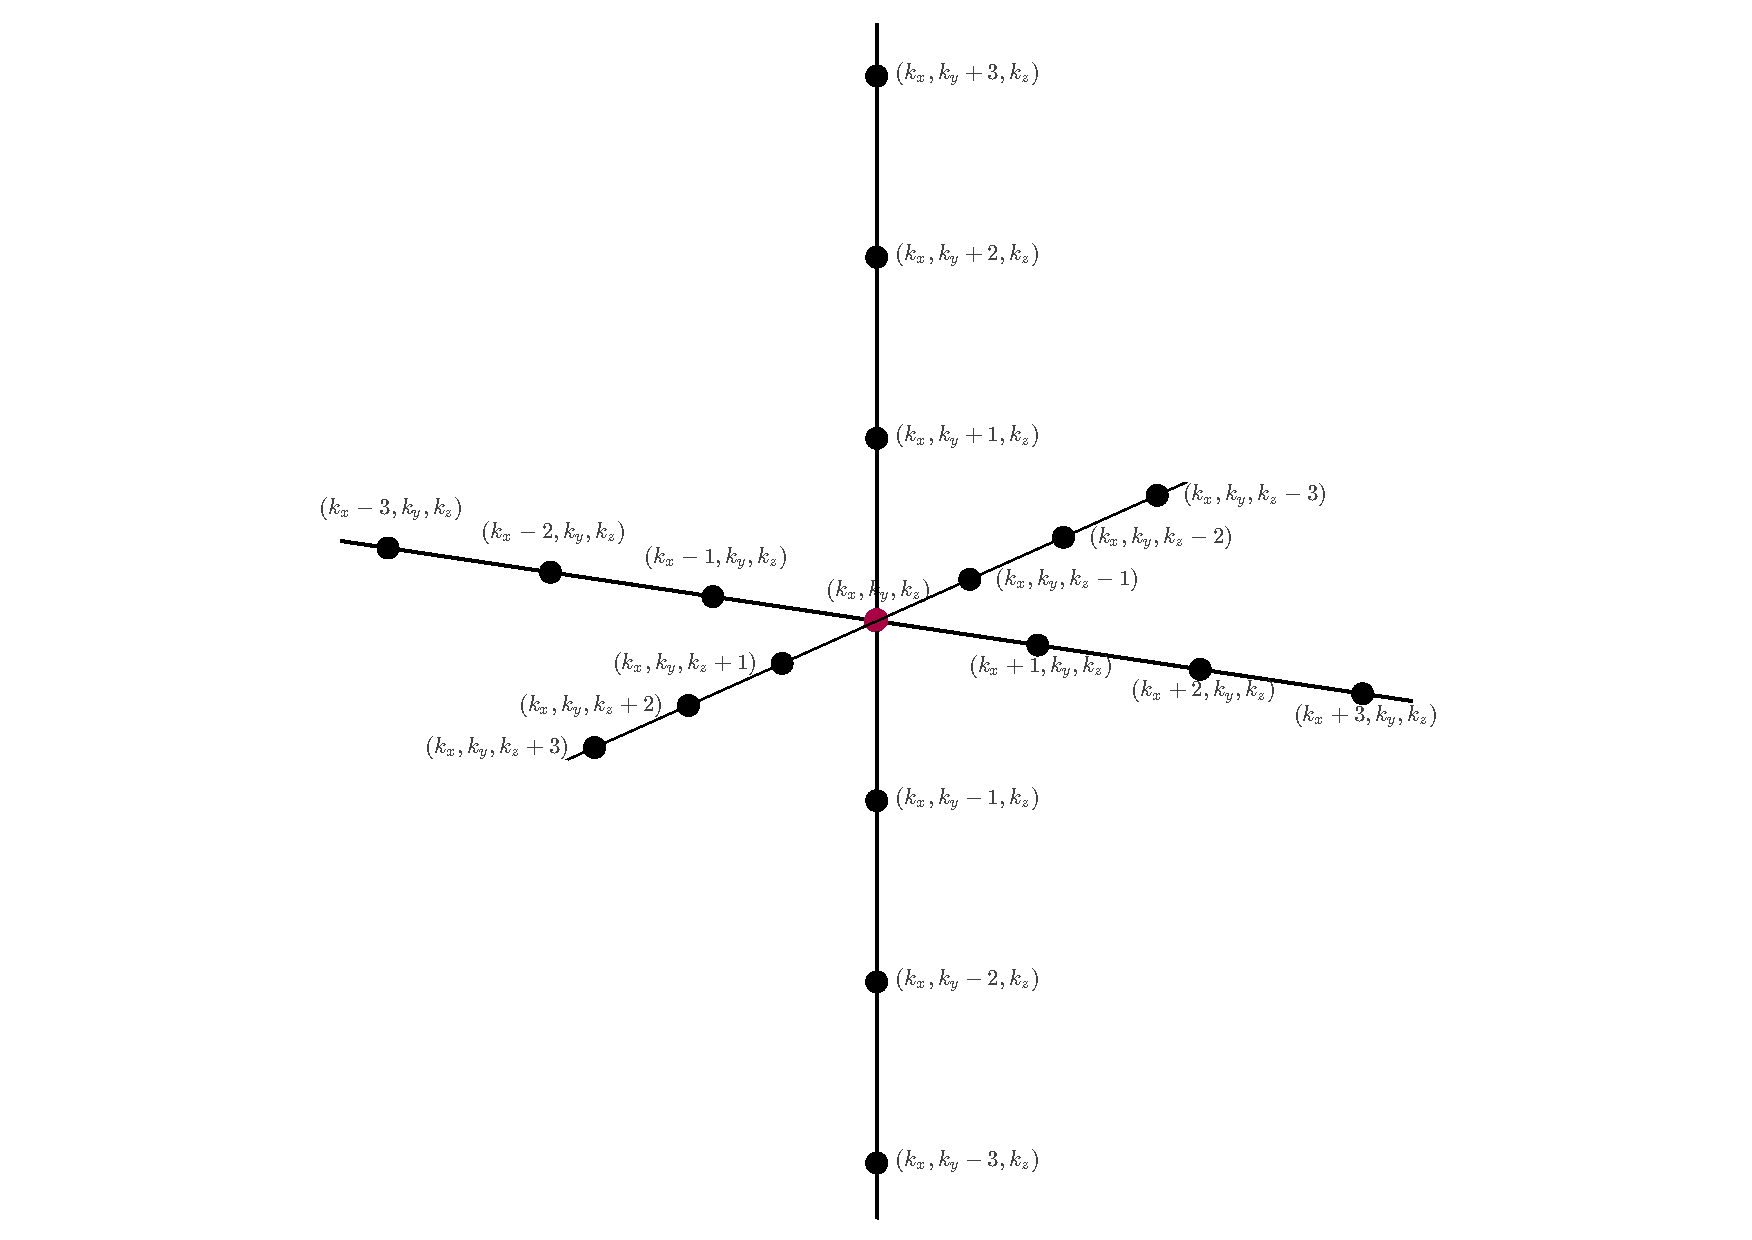
\includegraphics[width=0.9\textwidth]{\localPath/figures/stencil.pdf}
  \caption{Présentation des \emph{stencils} utilisés par la méthode WENO5 pour calculer le flux numérique.}
  \label{fig:intro:stencil}
\end{figure}

La méthode WENO5 consiste en 3 interpolations, sur 3 \emph{stencils} différents, comme l'illustre la figure~\ref{fig:intro:stencil}, pondérées par des poids non-linéaires issus des approximations des dérivées successives de $f$. L'écriture des poids s'effectue comme suit dans le cas $f^-=0$ :
$$
  \begin{aligned}
    \beta_0 &= \frac{13}{12}( \underbrace{f^+_{j-2} - 2f^+_{j-1} + f^+_{j}}_{\Delta x^2(f''_{j} + \mathcal{O}(\Delta x))})^2   + \frac{1}{4}( \underbrace{  f^+_{j-2} - 4f^+_{j-1} + 3f^+_{j}  }_{ 2\Delta x ( f'_{j} + \mathcal{O}(\Delta x^2))})^2 \\
    \beta_1 &= \frac{13}{12}( \underbrace{f^+_{j-1} - 2f^+_{j}   + f^+_{j+1}}_{\Delta x^2(f''_{j} + \mathcal{O}(\Delta x^2))} )^2 + \frac{1}{4}( \underbrace{  f^+_{j-1} -               f^+_{j+1}}_{ 2\Delta x   f'_{j} + \mathcal{O}(\Delta x^2))})^2 \\
    \beta_2 &= \frac{13}{12}( \underbrace{f^+_{j}   - 2f^+_{j+1} + f^+_{j+2}}_{\Delta x^2(f''_{j} + \mathcal{O}(\Delta x))} )^2   + \frac{1}{4}( \underbrace{ 3f^+_{j}   - 4f^+_{j+1} +  f^+_{j+2}}_{-2\Delta x ( f'_{j} + \mathcal{O}(\Delta x^2))})^2 \\
  \end{aligned}
$$
où les coefficients $\beta_0$ sont appelés indicateurs de continuité (\emph{indicators of smoothness}). Ce qui nous permet de calculer les poids définis par :
$$
  \alpha_i = \frac{\gamma_i}{(\varepsilon + \beta_i)^2},\quad i=0,1,2
$$
où $\varepsilon$ est un paramètre numérique pour assurer la non nullité du dénominateur, il sera pris à $10^{-6}$ ; et avec $\gamma_0=\frac{1}{10}$, $\gamma_1=\frac{6}{10}$ et $\gamma_2=\frac{3}{10}$. La normalisation des poids s'effectue comme suit :
$$
  w_i = \frac{\alpha_i}{\sum_m \alpha_m},\quad i=0,1,2
$$
Nous pouvons ensuite calculer les flux numériques pour WENO5 \cite{Shu:2003}, donnés par :
$$
  \begin{aligned}
    \hat{f}_{j+\frac{1}{2}}^+   =\ & w_0\left(  \frac{2}{6}f^+_{j-2} - \frac{7}{6}f^+_{j-1} + \frac{11}{6}f^+_{j}   \right)
                                +    w_1\left( -\frac{1}{6}f^+_{j-1} + \frac{5}{6}f^+_{j}   +  \frac{2}{6}f^+_{j+1} \right) \\
                                +  & w_2\left(  \frac{2}{6}f^+_{j}   + \frac{5}{6}f^+_{j+1} -  \frac{1}{6}f^+_{j+2} \right).
  \end{aligned}
$$
La méthode WENO5 prend la forme finale :
$$
  \partial_xf(x_j) \approx \frac{1}{\Delta x}\left[ \left(\hat{f}_{j+\frac{1}{2}}^+ - \hat{f}_{j-\frac{1}{2}}^+ \right) + \left(\hat{f}_{j+\frac{1}{2}}^- - \hat{f}_{j-\frac{1}{2}}^- \right) \right].
$$

Il existe des variantes de la méthode WENO5, permettant de réduire la perte d'ordre à l'approche d'un choc, à savoir WENO-M (\cite{Henrick:2005}) ou WENO-Z (\cite{Borges:2008}). Ces variations se font sur le calcul des poids non-linéaires. Ainsi la méthode WENO-M utilise une fonction de \emph{mappage} pour équilibrer les poids et est définie par :
$$
  \begin{aligned}
    \alpha_i    &= \frac{\gamma_i}{(\epsilon + \beta_i)^2} \\
    \tilde{w}_i &= \frac{\alpha_i}{\sum_k \alpha_k} \\
    g_i         &= w_i\left( \frac{\gamma_i + \gamma_i^2 - 3w_i\gamma_i + w_i^2}{\gamma_i^2 + w_i(1-2\gamma_i)} \right) \\
    w_i         &= \frac{g_i}{\sum_k g_k}
  \end{aligned}
$$
avec le paramètre $\epsilon = 10^{-4}$. La méthode WENO-Z est quant à elle définie par :
$$
  \begin{aligned}
    \alpha_i &= \gamma_i\left( 1+ \frac{\tau_5}{\epsilon + \beta_i} \right) \\
    w_i      &= \frac{\alpha_i}{\sum_k \alpha_k}
  \end{aligned}
$$
avec les paramètres $\epsilon = 10^{-40}$ et $\tau_5 = \beta_0 - \beta_2$. Cette dernière méthode est celle qui réduit le plus la perte d'ordre à l'approche d'une discontinuité. L'étude approfondie de ces méthodes n'est pas envisagée dans ce travail car les solutions de la physique des plasmas ne présentent pas de discontinuités. Il est à noter que ces méthodes conservent la même linéarisation que le schéma WENO5 classique de Jiang et Shu~\cite{Jiang:1996}, ce qui permet d'y appliquer les résultats de stabilités obtenus dans le chapitre~\ref{chap1}.

Il est possible de monter en ordre en suivant les résultats dans~\cite{Wu:2021}, l'ordre 5 sera considéré comme suffisant dans la suite de ce travail.

L'étude de la stabilité de la méthode WENO5 couplée avec différentes méthodes de type Runge-Kutta pour la résolution en temps a été initiée dans~\cite{Wang:2007} où il a été démontré l'instabilité de la méthode couplée avec la méthode d'Euler explicite, il est nécessaire d'avoir au moins un étage supplémentaire permettant d'assurer la stabilité, ou d'utiliser une méthode d'ordre 3. Des estimations de stabilité et de conditions de stabilité ont par la suite été proposées dans \cite{Motamed:2010,Lunet:2017}. Une étude automatique de la stabilité est présentée dans~\cite{Crouseilles:2019b} qui constitue le chapitre~\ref{chap1} de ce document.

% --------------------------------------------------------------------
\subsection{Méthode semi-lagrangienne}
% --------------------------------------------------------------------

Une méthode très populaire pour la résolution numérique de l'équation de Vlasov est la méthode semi-lagrangienne. Celle-ci s'adapte très bien à notre problème car les termes de transports sont linéaires. Elle a l'avantage de ne pas introduire de contrainte de stabilité. La méthode semi-lagrangienne repose sur la remonté des caractéristique, prenons pour exemple l'équation :
$$
  \partial_t u + a\partial_xu = 0,\quad u(t=0,x)=u_0(x),
$$
ce qui correspond à l'équation~\ref{eq:0:dtudxfu} avec le flux $f$ linéaire par rapport à l'inconnue $u$. On définit les caractérisitique le long desquelles $u$ est constante :
$$
  \begin{cases}
    \dot{x}(s) = a \\
    x(t) = x
  \end{cases}
$$
dont la solution s'écrit $x(s) = a(s-t)+x$. Avec $u(s,x(s))=u(t,x(t))$ on a $u(s,a(s-t)+x) = u(t,x)$ et en prenant $s=t^n=n\Delta t$, et $t=t^{n+1}$, on a :
$$
  u(t^{n+1},x) = u(t^n,x-a\Delta t),\quad \forall x\in[0,L]
$$
Pour connaître $u(t^{n+1},x_j)$ de $u(t^n,\cdot)$, on pose $x=x_j$ : $u(t^{n+1},x_j) = u(t^n,x_j-a\Delta t)$, comme l'illustre la figure~\ref{fig:intro:semilag}. Dans le cadre d'un schéma numérique, $x_j-a\Delta t$ n'étant pas un point de la grille, il faut évaluer en $x_j-a\Delta t$ un polynôme par morceaux, construit à partir des données $u(t^n,x_k)$, $k\in\mathbb{N}$. Plusieurs méthodes d'interpolation sont alors envisageable, la méthode par splines permet une reconstruction gloable de la solution~\cite{Cheng:1976,Sonnendrucker:2015} ; une approche plus locale à partir des données d'un \emph{stencil}, c'est-à-dire des données $u(x_{j^\star-d},t^n)$ jusqu'à $u(x_{j^\star+d},t^n)$, à l'aide d'un polynôme d'interpolation, comme un polynôme de Lagrange de degré $2d+1$, est aussi envisageable~\cite{Charles:2013}. Nous utiliserons cette approche locale avec $d=2$ par la suite.

\begin{figure}[h]
  \centering
  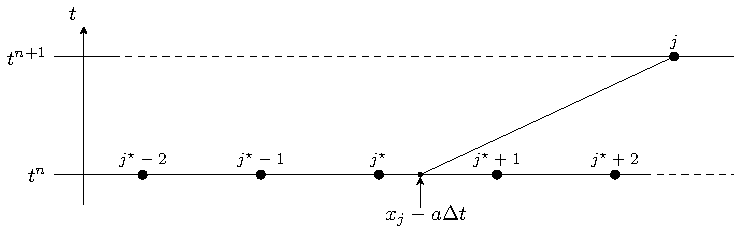
\includegraphics[width=0.9\textwidth]{\localPath/figures/semilag.pdf}
  \caption{Méthode des caractéristiques pour une méthode semi-lagrangienne avec une vitesse de transport $a>0$, et $d=2$.}
  \label{fig:intro:semilag}
\end{figure}


% --------------------------------------------------------------------
\subsection{Méthode pseudo-spectrale}
% --------------------------------------------------------------------

Une autre méthode souvent utilisée pour la résolution d'équations aux dérivées partielles est la méthode pseudo-spectrale qui consiste à approcher les opérateurs différentiels dans l'espace de Fourier à l'aide de transformées de Fourier. Cette méthode permet de transformer une équation aux dérivées partielles en un système d'équations différentielles ordinaires en transformant par exemple une dérivée dans l'espace réel en un produit dans l'espace de Fourier. Nous considèrerons ici la transformée de Fourier discrète, cela consiste à réécrire notre fonction $u$, $L$-périodique et de classe $C^1$, sous la forme :
$$
  u(x) = \sum_{\kappa=-\infty}^{+\infty} \hat{u}_\kappa e^{i\frac{2\pi \kappa}{L}x},
$$
où les coefficients de Fourier $\hat{u}_\kappa$ sont définis par :
$$
  \hat{u}_\kappa = \frac{1}{L}\int_0^L u(x)e^{-i\frac{2\pi \kappa}{L}x}\dd{x}.
$$

En n'ayant la connaissance de la fonction $u$ qu'en des points $x_j = j\frac{L}{N}$, $j=0,\dots,N-1$ de la grille, il est possible d'approcher les coefficient de Fourier par une somme discrète :
$$
  \hat{u}_\kappa \approx \frac{1}{N-1}\sum_{j=0}^N u(x_j) e^{=i\frac{2\pi j}{N}\kappa}.
$$

Transformer une dérivée en un produit nous sera utile au long de ce travail dans deux contextes, un premier linéaire :
$$
  \partial_t u + a\partial_x u = 0,\qquad u(t=0,x)=u_0(x)
$$
devenant après une transformée de Fourier : $\partial_t \hat{u}_\kappa + ai\kappa \hat{u}_\kappa = 0$ et pouvant se résoudre exactement en temps : $\hat{u}_\kappa(t) = \exp(-ia\kappa t)\hat{u}_\kappa(0)$. Cela correspond à la partie linéaire d'une méthode de Lawson~\ref{ssec:0:lawson}. L'autre cas d'utilisation sera pour un terme non-linéaire de la forme :
$$
  \partial_t u + \partial_xf(u) = 0,\qquad u(t=0,x)=u_0(x)
$$
devenant alors après une transformée de Fourier : $\partial_t\hat{u}_\kappa + i\kappa\widehat{\left(f(u)\right)}_\kappa = 0$. Ce terme n'ayant pas de solution explicite il sera résolu numériquement pas une méthode Runge-Kutta, correspondant au terme non-linéaire d'une méthode de Lawson.

Nous utiliserons l'algorithme de transformée de Fourier rapide (\emph{fast Fourier transform} ou FFT) pour effectuer numériquement cette opération, dont une implémentation est proposée dans~\cite{Saramito:2013}. Cet algorithme possède une complexité en temps de $\order{N\log N}$, où $N$ est le nombre de points de discrétisation en espace.

%% section 4
% !TEX root = ../../main.tex

\section{Relations de dispersion}
\label{s:dispersion}

Cette section est dédiée à l'étude des relations de dispersion relatives aux modèles cinétique~\eqref{eq:vlasov}-\eqref{eq:poisson} et hybride linéarisé~\eqref{eq:vahl}. Il s'agit de linéariser le modèle étudié puis d'exprimer le mode fondamental du champ électrique linéarisé. Cela permet d'obtenir une très bonne approximation de la phase linéaire de l'énergie électrique. Cette approche, complètement indépendante des schémas numériques utilisés pour résoudre le modèle de départ, sera utilisée comme outil de validation des codes présentés dans la section~\ref{s:scheme}.

Nous allons présenter les relations de dispersion de nos deux modèles, puis nous expliquerons comment reconstruire l'approximation linéaire de l'énergie électrique. Enfin, nous détaillerons les calculs des relations de dispersion pour le cas test qui nous intéressera dans les simulations numériques (sections~\ref{s:limit} et~\ref{s:compare}).

%----------
\subsection{Relations de dispersion dans le cas cinétique}
%----------

Nous nous intéressons d'abord aux relations de dispersion du modèle cinétique de Vlasov-Poisson~\eqref{eq:vlasov}-\eqref{eq:poisson}, en nous appuyant sur \cite{Sonnendrucker:2015}. Pour obtenir les relations de dispersion, il est nécessaire de linéariser le système autour d'un équilibre, pour cela rappelons les équations de Vlasov-Poisson~\eqref{eq:vlasov}-\eqref{eq:poisson} :
\begin{equation}
  \begin{cases}
    \partial_t f + v\partial_xf + E\partial_vf = 0 \\
    \partial_x E = \int_\mathbb{R} f\,\mathrm{d}v - 1 \\
    f(t=0, x, v)=f^0(x,v)
  \end{cases}
  \label{eq:vp}
\end{equation}
Dans un premier temps, nous nous intéressons à la linérarisation de ce modèle cinétique autour d'un état d'équilibre donné par $\left(f(t,x,v)\right)_{eq} = f^{(0)}(v)$ et $\left(E(t,x)\right)_{eq} = 0$, on considère le développement suivant :
\begin{equation}
  \begin{cases}
    f(t,x,v) = f^{(0)}(v) + \varepsilon f^{(1)}(t,x,v) + \mathcal{O}(\varepsilon^2) \\
    E(t,x) = 0 + \varepsilon E^{(1)}(t,x) + \mathcal{O}(\varepsilon^2)
  \end{cases}
  \label{eq:expansions}
\end{equation}
La densité de particules est définie par $\rho_0 = \rho_{0,c}+\rho_{0,h} = \int f^{(0)}\,\mathrm{d}v$. On injecte~\eqref{eq:expansions} dans~\eqref{eq:vp} pour obtenir :
$$
  \begin{cases}
    \varepsilon\partial_t f^{(1)} + v\varepsilon\partial_x f^{(1)} + \varepsilon E^{(1)}\left(\partial_v f^{(0)}+\varepsilon\partial_v f^{(1)}\right)=\mathcal{O}(\varepsilon^2) \\
    \varepsilon\partial_x E^{(1)} = \int f^{(0)} + \varepsilon\int f^{(1)} - n_0 + \mathcal{O}(\varepsilon^2)
  \end{cases}
$$
ce qui nous permet d'obtenir, en négligeant les termes d'ordre $\varepsilon^2$, le système de Vlasov-Poisson linéarisé :
\begin{equation}
  \begin{cases}
    \partial_t f^{(1)} + v\partial_x f^{(1)} + E^{(1)}\partial_v f^{(0)} = 0 \\
    \partial_x E^{(1)} = \int f^{(1)}\,\mathrm{d}v
  \end{cases}
  \label{eq:systVPlin}
\end{equation}

Pour un état d'équilibre connu $f^{(0)}(v)$, habituellement une distribution gaussienne, les inconnues de~\eqref{eq:systVPlin} sont $f^{(1)}(t,x,v)$ et $E^{(1)}(t,x)$.

Nous souhaitons dériver l'expression générale de la relation de dispersion associée au modèle cinétique linéarisé~\eqref{eq:systVPlin}. Afin de simplifier la lecture, nous supprimons l'index $(1)$ sur nos inconnues $f^{(1)}$ et $E^{(1)}$. Nous supposons que le fonctions $f^{(1)}$ et $E^{(1)}$ sont $L$-périodiques en $x$ dans le domaine $\Omega=[0,L]$, nous allons, successivement, appliquer une transformée de Fourier en $x$ et et une transformée de Laplace en $t$ sur le système~\eqref{eq:systVPlin}.

Tout d'abord, nous effectuons une transformée de Fourier en $x$, définie pour une fonction $f(x)$ comme :
$$
  \hat{f}(k) = \frac{1}{L}\int_0^L f(x)e^{-ikx}\,\mathrm{d}x\,,\quad k=\frac{2\pi}{L}n, n\in\mathbb{Z}
$$
Nous obtenons :
\begin{equation}
  \begin{cases}
    \partial_t \hat{f} + ikv\hat{f} + \hat{E}\partial_v f^{(0)} = 0 \\
    ik\hat{E} = \int \hat{f}(t,k,v) dv
  \end{cases}
  \label{eq:fourier}
\end{equation}
Maintenant, nous utilisons la transformée de Laplace définie pour une fonction $f(t)$ par :
$$
  \tilde{f}(\omega) = \int_0^{+\infty} f(t)e^{i\omega t}\,\mathrm{d}t
$$
et, si elle est définie, la transformée de Laplace inverse est donnée par :
$$
  f(t) = \frac{1}{2i\pi}\int_{u-i\infty}^{u+i\infty} \tilde{f}(\omega)e^{-i\omega t}\,\mathrm{d}\omega
$$
Appliquons la transformée de Laplace à la première équation du système~\eqref{eq:fourier} :
$$
  \int_0^{+\infty}\partial_t\hat{f}(t)e^{i\omega t}\,\mathrm{d}t
  + \int_0^{+\infty}ikv\hat{f}(t)e^{i\omega t}\,\mathrm{d}t
  + \int_0^{+\infty}\hat{E}(t)\partial_v f^{(0)}e^{i\omega t}\,\mathrm{d}t
  = 0
$$
et en utilisant une intégration par partie dans la première intégrale nous obtenons :
$$
  \begin{aligned}
    -\hat{f}(t=0,k,v) - i\omega\int_0^{+\infty} \hat{f}(t)e^{i\omega t}\,\mathrm{d}t + ikv\int_0^{+\infty} \hat{f}(t)e^{i\omega t} \mathrm{d}t \\
    +\partial_vf^0\int_0^{+\infty}\hat{E}(t)e^{i\omega t}\,\mathrm{d}t=0
  \end{aligned}
$$
et donc :
\begin{equation}
  (ikv-i\omega)\tilde{\hat{f}}(\omega,k,v) + \partial_vf^0\tilde{\hat{E}}(\omega,k) = \hat{f}_0(k,v),
  \label{eq:fourierlaplace_f}
\end{equation}
où $\hat{f}_0(k,v) = \hat{f}(t=0,k,v)$ correspond à la condition initiale. En appliquant maintenant la transformée de Laplace à la seconde équation de~\eqref{eq:fourier} nous obtenons :
$$
  \int_0^{+\infty}ik\hat{E}(t,k)e^{i\omega t}\,\mathrm{d}t = \int_0^{+\infty}\int_{-\infty}^{+\infty}\hat{f}(t,k,v)\,\mathrm{d}v\,e^{i\omega t}\,\mathrm{d}t
$$
ce qui nous donne :
\begin{equation}
  \tilde{\hat{E}}(\omega,k)=-\frac{i}{k}\int_{-\infty}^{+\infty}\tilde{\hat{f}}(\omega,k,v)dv
  \label{eq:fourierlaplace_E}
\end{equation}
Maintenant, nous souhaitons injecter l'équation~\eqref{eq:fourierlaplace_f} dans~\eqref{eq:fourierlaplace_E}. Nous devons prêter attention aux pôles $\omega = kv$. En fait, si $\Im(\omega)>0$ et pour une fonction analytique $g(v)$, alors l'intégrale $\int_{-\infty}^{+\infty}\frac{g(v)}{ikv-i\omega}\,\mathrm{d}v$ est analytique. Lorsque $\Im(\omega) \leq 0$, nous devons construire un prolongement analytique et remplacer l'intégrale par $\int_\gamma \frac{g(v)}{ikv-i\omega}\,\mathrm{d}v$ avec $\gamma$ un coutour ouvert parallèle à l'axe réel à l'infini et qui passe par le pôle $\omega = kv$ (voir \cite{Sonnendrucker:2015}). Par la suite, nous utiliserons la notation $\gamma$ soit pour l'axe réel $]-\infty,+\infty[$ quand $\Im(\omega)>0$, ou pour un chemin ouvert bien choisi lorsque $\Im(\omega)\leq 0$. 

Avec cette notation, le résultat de l'injection de~\eqref{eq:fourierlaplace_f} dans~\eqref{eq:fourierlaplace_E} nous donne :
$$
  \begin{aligned}
    \tilde{\hat{E}}
    & = -\frac{i}{k}\int_\gamma \frac{1}{ikv-i\omega}\left( \hat{f}_0(k,v) - \partial_vf^{(0)}\tilde{\hat{E}}(\omega,k) \right)\,\mathrm{d}v \\
    & = -\frac{1}{k}\int_\gamma \frac{\hat{f}_0(k,v)}{kv-\omega}\,\mathrm{d}v + \frac{1}{k}\int_\gamma \frac{\partial_v f^{(0)}\tilde{\hat{E}}(\omega,k)}{kv-\omega}\,\mathrm{d}v \\
    & = - \frac{1}{k^2}\int_\gamma \frac{\hat{f}_0(k,v)}{v-\frac{\omega}{k}}\,\mathrm{d}v + \frac{1}{k^2}\tilde{\hat{E}}(\omega,k)\int_\gamma \frac{\partial_v f^{(0)}}{v-\frac{\omega}{k}}\,\mathrm{d}v
  \end{aligned}
$$
donc :
$$
  \left( 1 - \frac{1}{k^2}\int_\gamma \frac{\partial_v f^{(0)}}{v-\frac{\omega}{k}}\,\mathrm{d}v \right) \tilde{\hat{E}}(\omega,k) = -\frac{1}{k^2}\int_\gamma \frac{\hat{f}_0(k,v)}{v-\frac{\omega}{k}}\,\mathrm{d}v
$$
En introduisant :
\begin{equation}
  D(k,\omega) = 1 - \frac{1}{k^2}\int_\gamma \frac{\partial_v f^{(0)}}{v-\frac{\omega}{k}}\,\mathrm{d}v
  \label{eq:D}
\end{equation}
et
\begin{equation}
  N(k,\omega) = -\frac{1}{k^2}\int_\gamma\frac{\hat{f}_0(k,v)}{v-\frac{\omega}{k}}dv
  \label{eq:N}
\end{equation}
nous pouvons définir $\tilde{\hat{E}}(\omega,k)$ comme :
$$
  \tilde{\hat{E}}(\omega,k) = \frac{N(k,\omega)}{D(k,\omega)}
$$
L'équation~\eqref{eq:D} est appelée relation de dispersion du modèle cinétique.

%----------
\subsection{Relations de dispersion dans le cas hybride}
%----------

Intéressons-nous dans cette section à dériver l'expression générale de la relation de dispersion associée au modèle hybride linéarisé~\eqref{eq:vahl}. Pour cela, nous allons repartir du modèle hybride non-linéaire~\eqref{eq:hyb_nonlin} et linéariser à la fois les équations fluides et l'équation cinétique. On injecte le développement~\eqref{eq:lin_variables} dans~\eqref{eq:hyb_nonlin}. Les mêmes calculs que dans la section~\ref{s:models} et l'approximation en $\varepsilon^2$ y compris dans l'équation cinétique sur $f_h$ conduisent au modèle
$$
  \begin{cases}
    \partial_tu_c^{(1)}=E^{(1)}\\
    \partial_tE^{(1)}=-\rho_c^{(0)}u_c^{(1)}-\int v f_h^{(1)}\,\mathrm{d}v\\
    \partial_t f_h^{(1)}+ v\partial_xf_h^{(1)}+ E^{(1)}\partial_vf_h^{(0)}=0
  \end{cases}
$$ 
d'inconnues $E^{(1)}$, $u_c^{(1)}$ et $f_h^{(1)}$ que nous noterons dans la suite, respectivement, $E$, $u_c$ et $f_h$, solutions du système hybride linéarisé dans toutes les inconnues
\begin{equation}
  \begin{cases}
    \partial_t u_c = E \\
    \partial_t E = -\rho_c^{(0)}u_c - \int vf_h\,\mathrm{d}v \\
    \partial_t f_h + v\partial_x f_h + E\partial_v f_h^{(0)} = 0
  \end{cases}
\label{eq:systHlin}
\end{equation}
Nous insistons sur le fait que le modèle~\eqref{eq:systHlin} correspond à une linéarisation de la partie cinétique (ou chaude) du modèle hybride~\eqref{eq:vahl} que nous avons étudié précédemment. Par la suite, nous supposerons que la densité de particules froides $\rho_c^{(0)}$ est une constante (en temps $t$ et espace $x$) et que la fonction $f_h^{(0)}$ est une fonction paire en $v$ et ne dépend que de cette variable. Nous supposons que les fonctions $f_h$, $E$ et $u_c$ sont $L$-périodiques en $x$ sur le domaine spatial $\Omega = [0,L]$ et nous appliquons la transformée de Fourier en $x$ puis une transformée de Laplace en $t$.

Tout d'abord, nous appliquons la transformée de Fourier en $x$ :
\begin{equation}
  \begin{cases}
    \partial_t \hat{u}_c = \hat{E} \\
    \partial_t\hat{E}=-\rho_c^{(0)}\hat{u}_c-\int \hat{f}_h dv \\
    \partial_t \hat{f}_h+ikv\hat{f}_h+ \hat{E}\partial_v f_h^{(0)} = 0
  \end{cases}
  \label{eq:fourierH}
\end{equation}
Alors, nous multiplions par $e^{i\omega t}$ et nous intégrons en temps. L'équation sur $\hat{u}_c$ nous donne :
\begin{eqnarray}
  \int_0^{+\infty} \partial_t \hat{u}_c e^{i\omega t} \,\mathrm{d}t &=& \int_0^{+\infty} \hat{E}e^{i\omega t}\,\mathrm{d}t\nonumber\\
  -\int_0^{+\infty}i\omega  \hat{u}_c e^{i\omega t} \,\mathrm{d}t-\hat{u}_c(t=0,k) &=& \int_0^{+\infty} \hat{E}e^{i\omega t}\,\mathrm{d}t\nonumber\\
  -i\omega  \tilde{\hat{u}}_c(\omega,k)-\hat{u}_c(t=0,k) &=& \tilde{\hat{E}}(\omega,k)\nonumber\\
  \tilde{\hat{u}}_c(\omega,k)+\frac{1}{i\omega}\tilde{\hat{E}}(\omega,k) &=& -\frac{1}{i\omega}\hat{u}_c(t=0,k)
  \label{eq:LF_u}
\end{eqnarray}
Les mêmes opérations sur l'équation sur $\hat{E}$ nous donnent :
\begin{eqnarray}
  -i\omega  \tilde{\hat{E}}(\omega,k)-\hat{E}(t=0,k)&=&-\rho_c^{(0)}\tilde{\hat{u}}_c(\omega,k)-\int_{-\infty}^{+\infty} v\tilde{\hat{f}}_h(\omega,k)dv
  \label{eq:LF_E}
\end{eqnarray}
Tandis que l'équation sur $\hat{f}_h$ nous donne :
\begin{eqnarray}
  -i\omega  \tilde{\hat{f}}_h(\omega,k,v)-\hat{f}_h(t=0,k,v)+ikv\tilde{\hat{f}}_h(\omega,k,v)+\tilde{\hat{E}}(\omega,k)\partial_vf_h^{(0)}(v)=0\nonumber\\
  \tilde{\hat{f}}_h(\omega,k,v)\left(ikv-i\omega\right)=\hat{f}_h(t=0,k,v)-\tilde{\hat{E}}(\omega,k)\partial_vf_h^{(0)}(v)\nonumber\\
  \tilde{\hat{f}}_h(\omega,k,v)=-\frac{i}{k}\frac{\hat{f}_h(t=0,k,v)}{v-\frac{\omega}{k}}+\frac{i}{k}\frac{\tilde{\hat{E}}(\omega,k)\partial_vf_h^{(0)}(v)}{v-\frac{\omega}{k}}.
  \label{eq:LF_f}
\end{eqnarray}
Nous injectons l'expression~\eqref{eq:LF_f} dans~\eqref{eq:LF_E} :
$$
  \begin{aligned}
    -i\omega  \tilde{\hat{E}}(\omega,k)-\hat{E}(t=0,k)=-\rho_c^{(0)}\tilde{\hat{u}}(\omega,k)+\frac{i}{k}\int_\gamma v\frac{\hat{f}_h(t=0,k,v)}{v-\frac{\omega}{k}}dv \\
    -\frac{i}{k}\int_\gamma v\frac{\tilde{\hat{E}}(\omega,k)\partial_vf_h^{(0)}(v)}{v-\frac{\omega}{k}}dv
  \end{aligned}
$$
soit :
\begin{equation}
  \begin{aligned}
    \tilde{\hat{E}}(\omega,k)\left(1-\frac{1}{\omega k}\int_\gamma v\frac{\partial_vf_h^{(0)}(v)}{v-\frac{\omega}{k}}dv\right)-\frac{\rho_c^{(0)}}{i\omega}\tilde{\hat{u}}_c(\omega,k)=-\frac{1}{i\omega}\hat{E}(t=0,k)\nonumber\\
    -\frac{1}{\omega k}\int_\gamma v\frac{\hat{f}_h(t=0,k,v)}{v-\frac{\omega}{k}}dv
  \end{aligned}
  \label{eq:LF_Ef}
\end{equation}
Nous injectons maintenant l'expression~\eqref{eq:LF_u} dans~\eqref{eq:LF_Ef} pour obtenir le problème suivant :
$$
  \begin{aligned}
    \tilde{\hat{E}}(\omega,k)\left(1-\frac{1}{\omega k}\int_\gamma v\frac{\partial_vf_h^{(0)}(v)}{v-\frac{\omega}{k}}dv\right)+\frac{\rho_c^{(0)}}{i\omega}\left(\frac{1}{i\omega}\tilde{\hat{E}}(\omega,k)+\frac{1}{i\omega}\hat{u}_c(t=0,k)\right)\\
    =-\frac{1}{i\omega}\hat{E}(t=0,k)
    -\frac{1}{\omega k}\int_\gamma v\frac{\hat{f}_h(t=0,k,v)}{v-\frac{\omega}{k}}dv
  \end{aligned}
$$
soit :
$$
  \begin{aligned}
    \tilde{\hat{E}}(\omega,k)\left(1-\frac{1}{k^2}\left(\rho_c\frac{k^2}{\omega^2}+\int_\gamma \frac{\partial_vf_h^{(0)}(v)}{v-\frac{\omega}{k}}dv\right)\right)~~~~~~~~~~~~~~~~~~~~~~~~~~~~~~~~~~~~~~~~\\
    =\frac{\rho_c^{(0)}}{\omega^2}\hat{u}_c(t=0,k)-\frac{1}{i\omega}\hat{E}(t=0,k)
    -\frac{1}{\omega k}\int_\gamma v\frac{\hat{f}_h(t=0,k,v)}{v-\frac{\omega}{k}}dv
  \end{aligned}
$$
Nous introduisons :
\begin{equation}
  D(k,\omega) = 1-\frac{1}{k^2}\left( \rho_c^{(0)}\frac{k^2}{\omega^2}+\int_\gamma \frac{\partial_vf_h^{(0)}(v)}{v-\frac{\omega}{k}}dv\right )
  \label{eq:relD_H}
\end{equation}
et
\begin{equation}
  N(k,\omega) = \frac{\rho_c^{(0)}}{\omega^2}\hat{u}_c(t=0,k)-\frac{1}{i\omega}\hat{E}(t=0,k) 
    -\frac{1}{\omega k}\int_\gamma v\frac{\hat{f}_h(t=0,k,v)}{v-\frac{\omega}{k}}dv,
  \label{eq:relN_H}
\end{equation}
nous pouvons alors définir $\tilde{\hat{E}}(\omega,k)$ comme :
$$
  \tilde{\hat{E}}(\omega,k)=\frac{N(k,\omega)}{D(k,\omega)}
$$

\begin{remark}
  Comme nous le verrons dans la sous-section suivante, pour retrouver la pente de la partie linéaire de l'énergie électrique, il est suffisant de trouver les racines de $D(k,\omega)$, ou les pôles de $\tilde{\hat{E}}(\omega,k)$. Si seule la pente de la partie linéaire nous intéresse, un autre moyen de la retrouver est de réécrire les équations~\eqref{eq:LF_u}-\eqref{eq:LF_Ef} comme le système suivant :
  \begin{equation}
    \begin{pmatrix}
      1                       & \frac{1}{i\omega} \\
      -\frac{\rho_c}{i\omega} & 1-\frac{1}{\omega k}\int_\gamma v\frac{\partial_v f_h^{(0)}(v)}{v-\frac{\omega}{k}}\,\mathrm{d}v
    \end{pmatrix}
    \begin{pmatrix}
      \tilde{\hat{u}}_c(\omega,k) \\
      \tilde{\hat{E}}(\omega,k)
    \end{pmatrix}
    =
    \begin{pmatrix}
      -\frac{1}{i\omega}\hat{u}_c(0,k) \\
      -\frac{1}{i\omega}\hat{E}(0,k) - \frac{1}{\omega k}\int_\gamma v\frac{\hat{f}_h(0,k,v)}{v-\frac{\omega}{k}}\,\mathrm{d}v
    \end{pmatrix}
    \label{eq:systHyb}
  \end{equation}
  Le problème revient alors à trouver les racines du déterminant de ce système, qui s'écrit
%  Nous sommes alors incités à calculer le déterminant de ce système pour se faire une idée des solutions de ce système :
  $$
    \begin{aligned}
      Det(k,\omega) & = 1 - \frac{1}{\omega k}\int_\gamma v\frac{\partial_v f_h^{(0)}(v)}{v-\frac{\omega}{k}}\,\mathrm{d}v - \frac{\rho_c^{(0)}}{\omega^2} \\
                    & = 1 - \frac{1}{k^2}\left( \rho_c^{(0)}\frac{k^2}{\omega^2} + \int_\gamma \frac{\partial_v f_h^{(0)}(v)}{v-\frac{\omega}{k}}\,\mathrm{d}v \right)
    \end{aligned}
  $$
  On retrouve bien~\eqref{eq:relD_H}. La connaissance de~\eqref{eq:relN_H} nous donnera, en plus de la pente, la phase de l'énergie électrique dans sa partie linéaire.
\end{remark}

%----------
\subsection{Expression du champ électrique linéarisé}
%----------

Dans cette sous-section, nous considérons un prolongement analytique continu de $N(k,\omega)$ et $D(k,\omega)$, et nous supposons que la transformée de Laplace et de Fourier de $\tilde{\hat{E}}$ sont bien définies pour obtenir une approximation du champ électrique linéarisé.

La transformée de Laplace inverse peut être calculée à l'aide du théorème des résidus :
$$
  \hat{E}(t,k)=\frac{1}{2i\pi}\int_{u-i\infty}^{u+i\infty}\tilde{\hat{E}}(\omega,k)e^{-i\omega t}d\omega=\sum_jRes_{\omega=\omega^{k,j}}\left(\tilde{\hat{E}}(\omega,k)e^{-i\omega t}\right)
$$
où $\omega^{k,j}$ sont les pôles de $\tilde{\hat{E}}(\omega,k)$. Nous rappelons que si $\omega^{k,j}$ est un pôle simple, alors :
$$
  \begin{aligned}
    Res_{w=w^{k,j}}\left( \tilde{\hat{E}}(\omega,k)e^{-i\omega^{k,j}t} \right)
      & = \lim_{\omega\to\omega^{k,j}}\left( \omega - \omega^{k,j} \right)\tilde{\hat{E}}(\omega,k)e^{-i\omega t} \\
      & = \lim_{\omega\to\omega^{k,j}}\left( \omega - \omega^{k,j} \right)\frac{N(k,\omega)}{D(k,\omega)}e^{-i\omega t}
  \end{aligned}
$$
Maintenant, un développement de Taylor de $D(k,\omega)$ nous donne :
$$
  D(k,\omega) = \underbrace{D(k,\omega^{k,j})}_{0} + \left( \omega - \omega^{k,j} \right)\frac{\partial D}{\partial \omega}(k,\omega^{k,j}) + \mathcal{O}\left( (\omega-\omega^{k,j})^2 \right)
$$
donc, le passage à la limite nous donne :
\begin{equation}
  Res_{\omega=\omega^{k,j}}\left(\tilde{\hat{E}}(\omega,k)e^{-i\omega^{k,j}t}\right)=\frac{N(k,\omega^{k,j})}{\frac{\partial D}{\partial \omega}(k,\omega^{k,j})}e^{-i\omega^{k,j} t}.
  \label{eq:residu}
\end{equation}

\begin{remark}
  En fait, pour un $k$ fixé, on obtient une très bonne approximation de $\hat{E}(t,k)$ (excepté pour des temps courts) en considérant seulement la fréquence principale. Soient les deux racines $\omega^{k,j_0\pm}=\pm\omega_r+i\omega_i$ de $D(k,\omega)$ (où $\omega_r\in\mathbb{R}^+$, $\omega_i\in\mathbb{R}$) qui ont la plus grande partie imaginaire $\omega_i$ : pour toute autre racine $\omega^{k,j}$, on a $\Im(\omega^{k,j})<\omega_i$. Les autres pôles peuvent être négligés. En effet, nous avons :
  $$
    \begin{aligned}
       \hat{E}(t,k)&=&\sum_jC_je^{-i\omega^{k,j} t}=C_{j_0^+}e^{-i\omega^{k,j_0^+}t}+C_{j_0^-}e^{-i\omega^{k,j_0^-}t}+\sum_{j\neq j_0^\pm}C_je^{-i\omega^{k,j} t}\\
 &=&e^{\omega_it}\left(C_{j_0^+}e^{-i\omega_rt}+C_{j_0^-}e^{i\omega_rt}+\sum_{j\neq j_0^\pm}C_je^{-i\Re(\omega^{k,j}) t}e^{(\Im(\omega^{k,j})-\omega_i)t}\right)
    \end{aligned}
  $$
  et par hypothèse, $\Im(\omega^{k,j})-\omega_i < 0$ $\forall j\neq j_0^\pm$, nous pouvons conclure que la somme tend vers zéro lorsque $t\to+\infty$.
\end{remark}

\begin{lemma}
  Si $f^{(0)}(v)$ (respectivement $f_h^{(0)}(v)$) est une fonction paire, alors pour $D$ défini par~\eqref{eq:D} (respectivement~\eqref{eq:relD_H}) nous avons $D(k,\omega_r+i\omega_i) = 0 \Leftrightarrow D(k,-\omega_r+i\omega_i)=0$.
  \label{lemma:doubleracine}
\end{lemma}
\begin{proof}
  Voir en Annexe~\ref{a:dispersion}. \commentaire[Anais]{(à voir si on le laisse en annexe ou si on l'enlève complètement)} 
\end{proof}

En considérant seulement les deux racines principales $\pm\omega_r + i\omega_i$ de $D(k,\omega)$, supposés pôles simples de $\tilde{\hat{E}}(\omega,k)$, nous avons l'approximation :
$$
  \hat{E}(t,k)\approx Res_{\omega=\omega_r+i\omega_i}\left(\tilde{\hat{E}}(\omega,k)e^{-i\omega t}\right)+Res_{\omega=-\omega_r+i\omega_i}\left(\tilde{\hat{E}}(\omega,k)e^{-i\omega t}\right)
$$
où les résidus sont définis par~\eqref{eq:residu}. Notons $r^\pm$ le module de $\frac{N(k,\pm\omega_r+i\omega_i)}{\frac{\partial D}{\partial \omega}(k,\pm\omega_r+i\omega_i)}$ et $\phi^\pm$ son argument, nous avons alors :
\begin{equation}
  \hat{E}(t,k)\approx r^+e^{i\phi^+}e^{-i(\omega_r+i\omega_i)t}+r^-e^{i\phi^-}e^{-i(-\omega_r+i\omega_i)t}. 
  \label{eq:Etk_sanssym}
\end{equation}
Dans plusieurs cas test classiques, nous avons une symétrie entre les racines, qui dépend de la perturbation initiale de l'équilibre. Par la suite la perturbation initiale de l'équilibre sera toujours une fonction cosinus.

\begin{hyp}
  Le module et l'argument de $\frac{N(k,\pm\omega_r+i\omega_i)}{\frac{\partial D}{\partial \omega}(k,\pm\omega_r+i\omega_i)}$  vérifient $r^+ = r^-$ (noté $r$ par la suite) et $\phi^+ = -\phi^-$ (noté simplement $\phi$).
  \label{hyp:sym}
\end{hyp}
Sous l'hypothèse~\ref{hyp:sym}, nous obtenons :
\begin{eqnarray}
  \hat{E}(t,k)\approx&& re^{i\phi}e^{-i(\omega_r+i\omega_i)t}+re^{-i\phi}e^{-i(-\omega_r+i\omega_i)t} \nonumber\\
  &=&re^{\omega_i t}\left(e^{i(\omega_r t-\phi)}+e^{-i(\omega_r t-\phi)}\right)\nonumber\\
  &=&2re^{\omega_i t}\cos\left(\omega_r t-\phi\right).
  \label{eq:Etk}
\end{eqnarray}
Maintenant, si nous considérons la définition des coefficients de Fourier, nous avons :
$$
  \hat{E}(t,k) = \frac{1}{L}\int_0^L E(t,x)e^{-ikx}\,\mathrm{d}x = \frac{1}{L}\int_0^L E(t,x)\cos(-kx)\,\mathrm{d}x + i\frac{1}{L}\int_0^L E(t,x)\sin(-kx)\,\mathrm{d}x
$$
et :
$$
  \begin{aligned}
    \hat{E}(t,-k) 
      & = \frac{1}{L}\int_0^L E(t,x)e^{ikx}\,\mathrm{d}x = \frac{1}{L}\int_0^L\cos(kx)\,\mathrm{d}x + i\frac{1}{L}\int_0^L E(t,x)\sin(kx)\,\mathrm{d}x \\
      & = \frac{1}{L}\int_0^L E(t,x)e^{ikx}\,\mathrm{d}x = \frac{1}{L}\int_0^L\cos(-kx)\,\mathrm{d}x - i\frac{1}{L}\int_0^L E(t,x)\sin(-kx)\,\mathrm{d}x \\
      & = \overline{\hat{E}(t,k)}
  \end{aligned}
$$

\begin{hyp}
  $N(k,\omega) = 0$ si $k\notin\left\{\pm\frac{2\pi}{L}\right\}$.
  \label{hyp:knuls}
\end{hyp}
Sous l'hypothèse~\ref{hyp:knuls}, avec l'approximation des coefficients de Fourier (qui sont tous réels) données par~\eqref{eq:Etk} et avec $l=\frac{2\pi}{L}$, nous obtenons l'approximation du champ électrique suivante :
$$
  \begin{aligned}
    E(t,x) &\approx \varepsilon E^{(1)}(t,x) \approx \varepsilon\left( \hat{E}(t,l)e^{ikx} + \overline{\hat{E}(t,l)}e^{-ilx} \right) \\
           &\approx 2\varepsilon \hat{E}(t,l)\cos(lx) \\
           &\approx 4\varepsilon r e^{\omega_i t}\cos(\omega_t t -\phi)\cos\left(\frac{2\pi}{L}x\right)
  \end{aligned}
$$
Ce qui nous permet d'obtenir une approximation de l'énergie électrique, définie par :
\begin{equation}
  \begin{aligned}
    \mathcal{E}(t) & := \left( \int_0^L E^2(t,x)\,\mathrm{d}x \right)^{\frac{1}{2}} \\
                   & \approx 4\varepsilon r e^{\omega_i t}\left|\cos(\omega_rt - \phi)\right|\left( \int_0^L \cos^2\left(\frac{2\pi}{L}x\right)\,\mathrm{d}x \right)^{\frac{1}{2}} \\
                   & \approx 2\sqrt{2L}\varepsilon r e^{\omega_i t}\left|\cos(\omega_rt - \phi)\right|
  \end{aligned}
\label{eq:enelec}\end{equation}
puisque :
$$
  \begin{aligned}
    \int_0^L \cos^2\left(\frac{2\pi}{L}x\right)\,\mathrm{d}x
      & = \int_0^L\frac{1}{2}\,\mathrm{d}x + \int_0^L\frac{1}{2}\cos\left(\frac{4\pi}{L}x\right)\,\mathrm{d}x \\
      & = \frac{L}{2} + \left[ \frac{L}{8\pi}\sin\left(\frac{4\pi}{L}x\right)\right]_0^L = \frac{L}{2}
  \end{aligned}
$$

\begin{remark}
  Il est possible de mener une étude similaire pour une perturbation donnée par une fonction sinus. Nous obtenons alors des résultats similaires en remplaçant dans l'approximation de $\hat{E}(t,k)$, $E(t,x)$ et $\mathcal{E}(t)$ les fonctions cosinus par des fonctions sinus.
\end{remark}

Il est à noter que ces approximations ne prennent en compte que les racines dominantes de $D(\frac{2\pi}{L},\omega)$, les deux ayant la plus grande partie imaginaire. Cette approximation devient valable en temps $t$ suffisamment long.

La partie imaginaire $\omega_i$ nous donne le comportement global des coefficients de Fourier du champ électrique, et donc de l'énergie électrique comme une fonction du temps. Nous obtenons un amortissement de l'énergie électrique si $\omega_i < 0$, ou une instabilité si $\omega_i >0$. Lorsque nous traçons l'énergie électrique en fonction du temps en échelle logarithmique, nous pouvons observer les comportements suivants :
\begin{itemize}
  \item un amortissement avec un taux $\omega_i<0$, le taux indiquant la pente globale de l'amortissement,
  \item quelques oscillations stables, suivies du développement d'une instabilité avec un taux $\omega_i>0$, jusqu'à la saturation recherchée.
\end{itemize}

%----------
\subsection{Applications}\label{ssec:disp_appl}
%----------

Dans cette sous-section, nous nous intéressons au calcul de $D(k,\omega)$ pour le modèle cinétique~\eqref{eq:D} ou hybride~\eqref{eq:relD_H}, dans le cadre des cas tests qui nous intéressent. Pour le modèle cinétique la distribution initiale est donnée par :
$$
  f_0(x,v) = \mathcal{M}_{1-\alpha,0,T_c}(v)
    + \left(
      \mathcal{M}_{^\alpha/_2,v_0,1}(v) + \mathcal{M}_{^\alpha/_2,-v_0,1}(v)
    \right)(1+\epsilon\cos(kx))
$$
avec $\alpha$ la densité de particules chaudes, centrées en $\pm v_0\in\mathbb{R}$, et les particules froides sont caractérisées par une température $T_c$, et où l'on note :
$$
  \mathcal{M}_{\rho,u,T}(v) := \frac{1}{(2\pi T)^\frac{1}{2}}\exp\left(-\frac{|v-u|^2}{2T}\right)
$$
la distribution maxwellienne de densité $\rho$, centrée en la vitesse $u$ et de température $T$. Cette distribution initiale $f_0$ nous permet de construire une condition initiale compatible pour le modèle hybride, données par la limite $T_c\to 0$ :
\begin{equation}
  \begin{aligned}
    f_{h,0} (x,v) & = \left(
      \mathcal{M}_{^\alpha/_2,v_0,1}(v) + \mathcal{M}_{^\alpha/_2,-v_0,1}(v)
    \right)(1+\epsilon\cos(kx)) \\
    u_{c,0} & = 0
  \end{aligned}
\label{eq:f0hdexv}\end{equation}
le champ électrique à l'instant initial $E_0$ est donné par la résolution de l'équation de Poisson avec la condition initiale :
$$
  \partial_x E_0(x) = (1-\alpha) + \int_\mathbb{R}f_{h,0}(x,v)\,\mathrm{d}v - 1
$$

Nous cherchons ensuite les racines en $\omega$ de la fonction $D(k,\omega)$ pour $k$ fixé. Celles-ci sont approchées numériquement à l'aide d'une méthode de Newton, la dérivée $\frac{\partial D}{\partial\omega}(k,\omega)$ est alors nécessaire. La racine ayant la plus grande partie imaginaire, dans la pratique nous ne conservons que celle avec une partie réelle positive, nous donne des informations sur l'évolution de l'énergie électrique au cours du temps (taux d'amortissement et taux d'instabilité en échelle logarithmique). De plus, le calcul de $N(k,\omega)$ nous permet d'obtenir plus d'informations sur le mode dominant $\hat{E}(t,k)$ donné par~\eqref{eq:Etk_sanssym} dans le cas général, ou par~\eqref{eq:Etk} sous l'hypothèse~\ref{hyp:sym}. Nous en déduisons notamment la phase des oscillations de l'énergie électrique dans sa partie linéaire.


%-------------
\subsubsection{Quelques propriétés de la fonction de dispersion du plasma}

Dans le calcul de $D(k,\omega)$ et $N(k,\omega)$ apparaît la fonction de dispersion du plasma, aussi appelée fonction de Fried-Conte~\cite{Fried:1961} :
\begin{equation}
  Z(\xi):=\frac{1}{\sqrt{\pi}} \int_\gamma \frac{e^{-z^2}}{z-\xi}\,\mathrm{d}z
  \label{eq:Zfct}
\end{equation}
Tout d'abord on rappelle que :
\begin{equation}
  Z'(\xi)=-2\left(1+\xi Z(\xi)\right).
  \label{eq:Zder}
\end{equation}
Nous allons maintenant établir quelques propriétés utiles pour vérifier l'hypothèse~\ref{hyp:sym} dans différents cas test classiques.

\begin{lemma}
  La fonction $Z_\alpha^0(\omega):\omega\in\mathbb{C}\mapsto Z\left(\alpha\omega\right)\in\mathbb{C}$, avec $\alpha\in\mathbb{R}$ fixé, est telle que : $Z_\alpha^0(-\bar{\omega}) = -\overline{Z_\alpha^0(\omega)}$.
  \label{lemma:Z0}
\end{lemma}

\begin{lemma}
  La fonction $Z_{\alpha,\beta}^+(\omega):\omega\in\mathbb{C}\mapsto Z\left(\alpha\omega-\beta\right)+Z\left(\alpha\omega+\beta\right)\in\mathbb{C}$, avec $\alpha\in\mathbb{R}$, $\beta\in\mathbb{R}$ fixés, est telle que : $Z_{\alpha,\beta}^+\left(-\overline{\omega}\right)=-\overline{Z_{\alpha,\beta}^+(\omega)}$.
  \label{lemma:Z+}
\end{lemma}

\begin{lemma}
  La fonction $Z_{\alpha,\beta}^-(\omega):\omega\in\mathbb{C}\mapsto Z\left(\alpha\omega-\beta\right)-Z\left(\alpha\omega+\beta\right)\in\mathbb{C}$, avec $\alpha\in\mathbb{R}$, $\beta\in\mathbb{R}$ fixés, est telle que : $Z_{\alpha,\beta}^-\left(-\overline{\omega}\right)=\overline{Z_{\alpha,\beta}^-(\omega)}$.
  \label{lemma:Z-}
\end{lemma}

La démonstration de ces lemmes est proposée dans l'annexe~\ref{a:dispersion}.

L'introduction de la fonction $Z$ provient de la nécessité dans les relations de dispersion définies en~\eqref{eq:D}-\eqref{eq:N} et~\eqref{eq:relD_H}-\eqref{eq:relN_H} d'intégrer une distribution maxwellienne qui est une distribution gaussienne renormalisée :
$$
  \mathcal{M}_{\rho,u,T} = \frac{\rho}{\sqrt{2\pi T}}e^{-\frac{(v-u)^2}{2T}}
$$
Rappelons le résultat :
$$
  \partial_v \mathcal{M}_{\rho,u,T}(v) = -\frac{v-u}{T}\mathcal{M}_{\rho,u,T}(v)
$$
Ainsi, avant de passer à l'application de ces résultats sur le cas test qui nous intéresse, calculons une intégrale qui intervient dans le calcul de $D(k,\omega)$ :
$$
  \begin{aligned}
    \int_\gamma \frac{\partial_v\mathcal{M}_{\rho,u,T}}{v-\frac{\omega}{k}}\,\mathrm{d}v 
      & = -\frac{\rho}{\sqrt{2\pi T}T}\int_\gamma \frac{(v-\frac{\omega}{k} + \frac{\omega}{k}-u)e^{-\frac{(v-u)^2}{2T}}}{v-\frac{\omega}{k}}\,\mathrm{d}v \\
      & = -\frac{\rho}{\sqrt{2\pi T}T}\left( \int_\gamma e^{-\frac{(v-u)^2}{2T}}\,\mathrm{d}v + \left(\frac{\omega}{k}-u\right)\int_\gamma \frac{e^{-\frac{(v-u)^2}{2T}}}{v-\frac{\omega}{k}}\,\mathrm{d}v \right)
  \end{aligned}
$$
Dans la première intégrale, on utilise le changement de variable $w = \frac{v-u}{\sqrt{T}}$, $\mathrm{d}w = \frac{\mathrm{d}v}{\sqrt{T}}$, dans la seconde intégrale, nous utilisons le changement de variable suivant : $w=\frac{v-u}{\sqrt{2T}}$, $\mathrm{d}w = \frac{\mathrm{d}v}{\sqrt{2T}}$. Nous obtenons :
$$
  \begin{aligned}
    -\frac{\rho}{\sqrt{2\pi T}T}\left( \int_\gamma e^{-\frac{w^2}{2}}\sqrt{T}\,\mathrm{d}w + \left(\frac{\omega}{k}-u\right)\int_\gamma \frac{e^{-w^2}}{\sqrt{2T}w + u - \frac{\omega}{k}}\sqrt{2T}\,\mathrm{d}w \right) \\
    = \frac{\rho}{T}\left( 1 + \frac{1}{\sqrt{2\pi T}}\left(\frac{\omega}{k}-u\right)\int_\gamma \frac{e^{-w^2}}{w-\frac{1}{\sqrt{2T}}\left(\frac{\omega}{k}-u\right)}\,\mathrm{d}w \right)
  \end{aligned}
$$
et enfin nous obtenons :
\begin{equation}
  \int_\gamma \frac{\partial_v \mathcal{M}_{\rho,u,T}(v)}{v-\frac{\omega}{k}}\,\mathrm{d}v
    = -\frac{\rho}{T}\left( 1 + \frac{1}{\sqrt{2T}}\left(\frac{\omega}{k}-u\right)Z\left(\frac{\frac{\omega}{k}-u}{\sqrt{2T}}\right) \right)
    \label{eq:intforM}
\end{equation}
où $Z$ est la fonction de diffusion de plasma~\eqref{eq:Zfct}.

Le calcul de la fonction $N(k,\omega)$ demande l'évaluation d'une intégrale pour laquelle on utilise le changement de variable $w = \frac{v-u}{\sqrt{2T}}$,
$$
  \begin{aligned}
    \int_\gamma \frac{\mathcal{M}_{\rho,u,T}(v)}{v-\frac{\omega}{k}}\,\mathrm{d}v
      & = \frac{\rho}{\sqrt{2\pi T}}\int_\gamma \frac{e^{-\frac{(v-u)^2}{2T}}}{v-\frac{\omega}{k}}\,\mathrm{d}v \\
      & = \frac{\rho}{\sqrt{2\pi T}}\int_\gamma \frac{e^{-w^2}}{\sqrt{2T}w + u - \frac{\omega}{k}}\sqrt{2T}\,\mathrm{d}w \\
      & = \frac{\rho}{\sqrt{2\pi T}}\int_\gamma \frac{e^{-w^2}}{w - \frac{1}{\sqrt{2T}}\left(\frac{\omega}{k}-u\right)}\,\mathrm{d}w
  \end{aligned}
$$  
soit :
\begin{equation}
  \int_\gamma \frac{\mathcal{M}_{\rho,u,T}(v)}{v-\frac{\omega}{k}}\,\mathrm{d}v
    = \frac{\rho}{\sqrt{2T}}Z\left(\frac{\frac{\omega}{k}-u}{\sqrt{2T}}\right)
  \label{eq:NforM}
\end{equation}


%-------------
\subsubsection{Application à la modélisation hybride}

La condition initiale du cas test du modèle hybride nous donne comme état d'équilibre (état perturbé) pour les particules chaudes :
$$
  f_h^{(0)}(v) = \mathcal{M}_{^\alpha/_2,v_0,1}(v) + \mathcal{M}_{^\alpha/_2,-v_0,1}(v) = \frac{\alpha}{2\sqrt{2\pi}}\left( e^{-\frac{(v-v_0)^2}{2}} + e^{-\frac{(v+v_0)^2}{2}} \right)
$$
avec une vitesse des particules chaudes $v_0\in\mathbb{R}$ fixée et une densité de particules chaudes $\alpha\in\mathbb{R}$. Les particules froides n'étant pas perturbées, l'état d'équilibre est l'état initial caractérisé par une densité $\rho_c^{(0)}= 1-\alpha$, et une vitesse moyenne $u_c(t=0,x)=0$. L'expression~\eqref{eq:relD_H} nous donne à l'aide de~\eqref{eq:intforM} :
\begin{eqnarray}
  D(k,\omega)
    &=&1-\frac{1}{k^2}\left(\left(1-\alpha\right)\frac{k^2}{\omega^2}+\int_\gamma \frac{\partial_vf_h^{(0)}(v)}{v-\frac{\omega}{k}}dv\right)\nonumber\\
    &=&1-\frac{1}{k^2}\left[\left(1-\alpha\right)\frac{k^2}{\omega^2}-\frac{\alpha}{2}\left(1+\frac{1}{\sqrt{2}}\left(\frac{\omega}{k}-v_0\right)Z\left(\frac{1}{\sqrt{2}}\left(\frac{\omega}{k}-v_0\right)\right)\right)\right.\nonumber\\
    &&~~~~~~~~~~~~~~~~~~~\left.-\frac{\alpha}{2}\left(1+\frac{1}{\sqrt{2}}\left(\frac{\omega}{k}+v_0\right)Z\left(\frac{1}{\sqrt{2}}\left(\frac{\omega}{k}+v_0\right)\right)\right)\right].
  \label{eq:D_hchyb}
\end{eqnarray}
On dérive $D(k,\omega)$ à l'aide de~\eqref{eq:Zder} :
\begin{equation}
  \begin{aligned}
    \frac{\partial D(k,\omega)}{\partial \omega} = 2\frac{\left(1-\alpha\right)}{\omega^3}+\frac{1}{\sqrt{2}k^3}\frac{\alpha}{2}\left[\left(1-2\tilde{\omega}_-^2\right)Z\left(\tilde{\omega}_-\right)\right. \\
      \left.+\left(1-2\tilde{\omega}_+^2\right)Z\left(\tilde{\omega}_+\right)-2\tilde{\omega}_--2\tilde{\omega}_+\right]
  \end{aligned}
  \label{eq:hchybderD}
\end{equation}
où $\tilde{\omega}_\pm=\frac{1}{\sqrt{2}}\left(\frac{\omega}{k}\pm v_0\right)$.

Maintenant, remarquons que :
$$
  \hat{f}_h(t=0,k,v) = \hat{g}(k)\frac{\alpha}{2\sqrt{2\pi}}\left( e^{-\frac{(v-v_0)^2}{2}}  e^{-\frac{(v+v_0)^2}{2}}\right)\,,\quad g(x) = \cos\left(\frac{2\pi}{L}x\right)
$$
ce qui nous permet de simplifier ce calcul de $N(k,\omega)$ en utilisant~\eqref{eq:relN_H} et~\eqref{eq:NforM} :
$$
  \begin{aligned}
    N(k,\omega)
      & = \frac{(1-\alpha)}{\omega^2}\hat{u}(t=0,k) - \frac{1}{i\omega}\hat{E}(t=0,k) - \frac{\hat{g}(k)}{2\omega k}\left( \int_\gamma v\frac{\mathcal{M}_{^\alpha/_2,v_0,1}}{v-\frac{\omega}{k}}\,\mathrm{d}v  +  \int_\gamma v\frac{\mathcal{M}_{^\alpha/_2,-v_0,1}}{v-\frac{\omega}{k}}\,\mathrm{d}v \right) \\
      & = \frac{(1-\alpha)}{\omega^2}\hat{u}(t=0,k) - \frac{1}{i\omega}\hat{E}(t=0,k) - \frac{\hat{g}(k)}{2\omega k}\left( \int_\gamma\mathcal{M}_{^\alpha/_2,v_0,1}\,\mathrm{d}v + \frac{\omega}{k}\int_\gamma \frac{\mathcal{M}_{^\alpha/_2,v_0,1}}{v-\omega{k}}\,\mathrm{d}v\right. \\
      & \qquad\qquad\qquad\qquad\qquad\qquad\qquad\qquad\qquad\qquad \left. + \int_\gamma\mathcal{M}_{^\alpha/_2,-v_0,1}\,\mathrm{d}v + \frac{\omega}{k}\int_\gamma \frac{\mathcal{M}_{^\alpha/_2,-v_0,1}}{v-\omega{k}}\,\mathrm{d}v \right) \\
      & = \frac{(1-\alpha)}{\omega^2}\hat{u}(t=0,k) - \frac{1}{i\omega}\hat{E}(t=0,k) - \frac{\hat{g}(k)}{2\omega k}\left[ \alpha + \frac{\omega}{k}\frac{\alpha}{2\sqrt{2}}\left( Z\left(\frac{\frac{\omega}{k}-v_0}{\sqrt{2}}\right) \right.\right. \\
      & \qquad\qquad\qquad\qquad\qquad\qquad\qquad\qquad\qquad\qquad\qquad\qquad\quad + \left.\left.Z\left(\frac{\frac{\omega}{k}+v_0}{\sqrt{2}}\right) \right)\right]
  \end{aligned}
$$
soit finalement :
\begin{equation}
  \begin{split}
    N(k,\omega) = \frac{(1-\alpha)}{\omega^2}\hat{u}(t=0,k) - \frac{1}{i\omega}\hat{E}(t=0,k) \\
      -\frac{\hat{g}(k)}{k^2}\left[ \alpha\frac{k}{\omega} + \frac{\alpha}{2\sqrt{2}}\left( Z\left(\frac{\frac{\omega}{k}-v_0}{\sqrt{2}}\right) + Z\left(\frac{\frac{\omega}{k}+v_0}{\sqrt{2}}\right) \right) \right]
  \end{split}
  \label{eq:N_hchyb}
\end{equation}
où $\hat{g}(k)$ est donnée par :
\begin{equation}
  \hat{g}\left(\frac{2\pi}{L}\right) = \hat{g}\left(-\frac{2\pi}{L}\right) = \frac{1}{2}\,,\quad \hat{g}(k) = 0, k\notin\left\{-\frac{2\pi}{L} ,\frac{2\pi}{L} \right\}
\label{eq:gk}
\end{equation}

\begin{lemma}
  Sous l'hypothèse $\hat{u}(t=0,k)=0$, pour $\frac{\partial D(k,\omega)}{\partial\omega}$ donnée par~\eqref{eq:hchybderD} et $N(k,\omega)$ par~\eqref{eq:N_hchyb}, l'hypothèse~\ref{hyp:sym} est satisfaite.
  \label{lemme:hypcashyb}
\end{lemma}

La démonstration de ce lemme est effectuée dans l'annexe~\ref{a:dispersion}. Elle permet de justifier l'écriture~\eqref{eq:Etk} du mode fondamental du champ électrique linéarisé puis l'approximation~\eqref{eq:enelec} de l'énergie électrique linéarisée.

%-------------
\subsubsection{Application à la modélisation cinétique}

La densité de particules initiale de la modélisation cinétique peut se réécrire comme la somme de la densité de particules froides et de la densité de particules chaudes, avec pour les particules froides une simple distribution maxwellienne non perturbée, et pour les particules chaudes une bi-maxwellienne dont l'intégration a déjà été traitée dans le cas hybride :
\begin{equation}
  f_0(x,v) = \mathcal{M}_{1-\alpha,0,Tc}(v) + f_{h,0}(x,v)
 \label{init_f0_rel_disp} 
\end{equation}
avec $f_{h,0}(x,v)$ donnée par~\eqref{eq:f0hdexv}. L'expression de $D(k,\omega)$ s'obtient à partir de~\eqref{eq:D} et~\eqref{eq:intforM} :
\begin{equation}
  \begin{aligned}
    D(k,\omega) = 1 - \frac{1}{k^2}\left[\vphantom{\frac{}{\sqrt{}}}\right. & -\frac{1-\alpha}{T_c}\left( 1 + \frac{1}{\sqrt{2T_c}}\frac{\omega}{k}Z\left( \frac{1}{\sqrt{2T_c}}\frac{\omega}{k}\right) \right) \\
                                          & -\frac{\alpha}{2}\left( 1 + \frac{1}{\sqrt{2}}\left(\frac{\omega}{k}-v_0\right)Z\left(\frac{1}{\sqrt{2}}\left(\frac{\omega}{k}-v_0\right)\right) \right) \\
                                          & \left. -\frac{\alpha}{2}\left( 1 + \frac{1}{\sqrt{2}}\left(\frac{\omega}{k}+v_0\right)Z\left(\frac{1}{\sqrt{2}}\left(\frac{\omega}{k}+v_0\right)\right) \right)  \right]
  \end{aligned}
    \label{D_3bump}
\end{equation}
Expression que l'on peut dériver et simplifier à l'aide de~\eqref{eq:Zder} :
\begin{equation}
  \begin{aligned}
    \frac{\partial D(k,\omega)}{\partial\omega} = \frac{1}{\sqrt{2}k^3}\left[\vphantom{\frac{}{\sqrt{}}}\right.
        & \frac{1-\alpha}{\sqrt{T_c}T_c}\left( (1-2\tilde{\omega}_0^2)Z(\tilde{\omega}_0) - 2\tilde{\omega}_0 \right) \\
        & \left.\vphantom{\frac{}{\sqrt{}}} +\frac{\alpha}{2}\left( (1-2\tilde{\omega}_-^2)Z(\tilde{\omega}_-) + (1-2\tilde{\omega}_+^2)Z(\tilde{\omega}_+) - 2\tilde{\omega}_- - 2\tilde{\omega}_+ \right) \right]
  \end{aligned}
  \label{eq:3bumpderD}
\end{equation}
où $\tilde{\omega}_0 = \frac{1}{\sqrt{2T_c}}\frac{\omega}{k}$ et $\tilde{\omega}_\pm = \frac{1}{\sqrt{2}}(\frac{\omega}{k}\pm v_0)$. Maintenant, pour le calcul de $N(k,\omega)$, on remarque que l'on a :
$$
  \hat{f}(t=0,k,v) = \hat{g}(k) \frac{\alpha}{2\sqrt{2\pi}}\left( e^{-\frac{(v-v_0)^2}{2}} + e^{-\frac{(v+v_0)^2}{2}} \right) 
$$
avec la fonction $g(x)$ qui vérifie :
$$ 
  \hat{g}\left(\frac{2\pi}{L}\right) = \hat{g}\left(-\frac{2\pi}{L}\right) = \frac{1}{2}\,,\quad \hat{g}(k) = 0, k\notin\left\{-\frac{2\pi}{L} ,\frac{2\pi}{L} \right\}
$$
ce qui nous permet, en utilisant les équations~\eqref{eq:N} et~\eqref{eq:NforM} d'obtenir :
\begin{equation}
  N(k,\omega) = -\frac{\hat{g}(k)}{k^2}\frac{\alpha}{2\sqrt{2}}\left( Z\left(\frac{\frac{\omega}{k}-v_0}{\sqrt{2}}\right) + Z\left(\frac{\frac{\omega}{k}+v_0}{\sqrt{2}}\right) \right)
  \label{eq:N_3bump}
\end{equation}

Nous avons donc le lemme suivant.
\begin{lemma}
  Pour $\frac{\partial D(k,\omega)}{\partial\omega}$ donnée par~\eqref{eq:3bumpderD} et $N(k,\omega)$ par~\eqref{eq:N_3bump}, l'hypothèse~\ref{hyp:sym} est satisfaite.
  \label{lemme:hypcascin}
\end{lemma}

La démonstration de ce lemme est effectuée dans l'annexe~\ref{a:dispersion}. Elle permet de justifier l'écriture~\eqref{eq:Etk} du mode fondamental du champ électrique linéarisé puis l'approximation~\eqref{eq:enelec} de l'énergie électrique linéarisée. 

%----------
\subsubsection{Consistance des relations de dispersion}
%----------

%\commentaire[Nicolas]{
Dans les sous-sections précédentes, nous avons obtenu les relations de dispersion des modèles cinétique et VHL correspondant à la condition initiale \eqref{init_f0_rel_disp}. Une première validation va consister à vérifier que les relations de dispersion du modèle cinétique données par (\ref{D_3bump})-(\ref{eq:3bumpderD})-(\ref{eq:N_3bump}) sont consistantes, quand $T_c\to 0$, avec les relations de dispersion du modèle hybride données par (\ref{eq:D_hchyb})-(\ref{eq:hchybderD})-(\ref{eq:N_hchyb}). Pour cela, rappelons que 
$$
  Z(z)=\sqrt{\pi} \exp(-z^2) (i - erfi(z) )
$$
et qu'à la limite $z\to+\infty$, nous avons le développement asymptotique suivant 
$$
  erfi(z) = -i + \exp(z^2)/\sqrt{\pi} (\frac{1}{z} +\frac{1}{2z^3} +\frac{3}{4z^5} + \mathcal{O}\left(z^{-7}\right) ).
$$
Ainsi, nous avons $Z(z) =  2 i \sqrt{\pi} \exp(-z^2)  - \frac{1}{z}  - \frac{1}{2z^3} - \frac{3}{4z^5}+ \mathcal{O}\left(z^{-7}\right)$ ou encore $Z(z)= - \frac{1}{z}  - \frac{1}{2z^3}- \frac{3}{4z^5}+ \mathcal{O}\left(z^{-7}\right)$ et donc
$$
  zZ(z)=-1-\frac{1}{2z^2} + \mathcal{O}\left(z^{-4}\right).
$$
Commençons par regarder la consistance en $D(k,\omega)$. Avec $z=\frac{1}{\sqrt{2T_c}}\frac{\omega}{k}$ quand $T_c\to 0$, le terme correspondant aux particules froides de \eqref{D_3bump} s'écrit
\begin{eqnarray*}
  -\frac{1-\alpha}{T_c}\left(1+\frac{1}{\sqrt{2T_c}}\frac{\omega}{k}Z\left(\frac{1}{\sqrt{2T_c}}\frac{\omega}{k}\right)\right)&=&-\frac{1-\alpha}{T_c}\left(1-1-\frac{1}{2\left(\frac{1}{\sqrt{2T_c}}\frac{\omega}{k}\right)^2}+ \mathcal{O}\left(\left(\frac{1}{\sqrt{2T_c}}\frac{\omega}{k}\right)^{-4}\right)\right)\nonumber\\
  &=& \left(1-\alpha\right)\frac{k^2}{\omega^2} + \mathcal{O}(T_c). 
\end{eqnarray*}
C'est le terme correspondant à la partie fluide (froide) de \eqref{eq:D_hchyb}. Les autres termes (venant des particules chaudes) sont les mêmes dans les deux expressions, donc $D(k,\omega)$ donné par le modèle cinétique est consistant, à la limite $T_c\to 0$, avec celui donné par le modèle hybride (avec un taux $\mathcal{O}(T_c)$). Regardons ensuite la consistance en $\frac{\partial D(k,\omega)}{\partial \omega}$. Les termes venant des particules chaudes sont les mêmes dans les modèles cinétique (\ref{eq:3bumpderD}) et hybride (\ref{eq:hchybderD}). Nous ne nous intéressons qu'aux termes venant des particules froides. De (\ref{eq:3bumpderD}), nous avons
\begin{eqnarray*}
  &&\frac{1}{\sqrt{2}k^3}\frac{1-\alpha}{T_c\sqrt{T_c}}\left(Z\left(\tilde{\omega}_0\right)-2\tilde{\omega}_0^2Z\left(\tilde{\omega}_0\right)-2\tilde{\omega}_0\right)\\
  &=&\frac{1}{\sqrt{2}k^3}\frac{1-\alpha}{T_c\sqrt{T_c}}\left(-\frac{1}{\tilde{\omega}_0}-\frac{1}{2\tilde{\omega}_0^3}+2\tilde{\omega}_0+\frac{1}{\tilde{\omega}_0}+\frac{3}{2\tilde{\omega}_0^3}-2\tilde{\omega}_0\right)+\mathcal{O}\left(\tilde{\omega}_0^{-5}\right)\\
  &=&\frac{1}{\sqrt{2}k^3}\frac{1-\alpha}{T_c\sqrt{T_c}}\frac{1}{\tilde{\omega}_0^3}+\mathcal{O}\left(\tilde{\omega}_0^{-5}\right)
\end{eqnarray*}
donc pour $\tilde{\omega}_0=\frac{1}{\sqrt{2T_c}}\frac{\omega}{k}$, nous avons 
$$
  \frac{1}{\sqrt{2}k^3}\frac{1-\alpha}{T_c\sqrt{T_c}}\frac{2T_c\sqrt{2T_c}k^3}{\omega^3}=2\frac{1-\alpha}{\omega^3}
$$
qui est le terme fluide de \eqref{eq:hchybderD}. Regardons enfin la consistance en $N(k,\omega)$. Là encore, les termes venant des particules chaudes sont les mêmes dans les modèles cinétique (\ref{eq:N_3bump}) et hybride (\ref{eq:N_hchyb}). Les termes supplémentaires dans le modèle hybride s'annulent sous l'hypothèse $\hat{u}(t=0,k)=0$ et avec $\hat{g}(k)$ donné par (\ref{eq:gk}) et $\hat{E}(t=0,k)$ obtenu à partir de l'équation de Poisson 
\begin{eqnarray*}
  \partial_xE(t=0,x)&=& \rho_c(t=0,x)+\int f^h(t=0,x,v)dv-1\\
                    &=& \left(1-\alpha\right)+\alpha\left(1+\varepsilon\cos\left(\frac{2\pi}{L}x\right)\right)-1\\
                    &=& \alpha\varepsilon\cos\left(\frac{2\pi}{L}x\right)
\end{eqnarray*}
soit
\begin{equation}
  \hat{E}\left(t=0,k\right)=-\frac{i\alpha}{2k},~k\in\left\{-\frac{2\pi}{L},\frac{2\pi}{L}\right\},~~~\hat{E}(k)=0,~k\notin\left\{-\frac{2\pi}{L},\frac{2\pi}{L}\right\}.
\label{eq:Ekbis}
\end{equation}
La consistance du modèle cinétique, à la limite $T_c\to 0$, vers le modèle hybride est établie sur les relations de dispersion.
%} 
%Dans les sous-sections suivantes, nous faisons une étude numérique de la convergence pour $T_c\to 0$ du modèle cinétique \eqref{eq:vlasov}-\eqref{eq:poisson} vers le modèle hybride linéarisé \eqref{eq:vahl}.}


%% section 5
% !TEX root = ../../main.tex

\section{Limite du modèle cinétique vers le modèle hybride}
 \label{s:limit}

Il s'agit ici d'étudier numériquement la convergence du modèle cinétique \eqref{eq:vlasov}-\eqref{eq:poisson} vers le modèle VHL \eqref{eq:vahl}, lorsque la température $T_c$ des particules froides tend vers 0. Une première étude de consistance est effectuée sur les relations de dispersion. Une seconde étude, numérique, montre la convergence de différentes quantités obtenues par les schémas proposés dans la section \ref{s:scheme}. Ces deux études complémentaires ont pour but de justifier l'utilisation de la modélisation hybride linéarisée lorsque les particules se répartissent en deux faisceaux: l'un de particules chaudes (rapides) et l'autre de particules froides (de température $T_c\ll 1$, lentes). Pour cela, le modèle cinétique \eqref{eq:vlasov}-\eqref{eq:poisson} sera initialisé avec
\begin{equation}
  f^0(x,v) = \mathcal{M}_{1-\alpha,0,T_c}(v) + (1+\epsilon\cos(kx))\left( \mathcal{M}_{^\alpha/_2,v_0,1}(v) + \mathcal{M}_{^\alpha/_2,-v_0,1}(v) \right)
\label{eq:K:init}
\end{equation}
avec $k = 0.5$, $v_0 = 3.4$, $\alpha=0.2$, $x\in[0,L]$, $L=\frac{2\pi}{k}=2\pi$, $v\in[-v_{\text{max}},v_{\text{max}}]$ avec $v_{\text{max}}=12$ et la perturbation des particules chaudes $\epsilon = 10^{-2}$. Le paramètre $T_c$ prendra différentes valeurs selon les résultats que nous souhaitons illustrer. Comme dans la sous-section \ref{ssec:disp_appl}, on a noté  $\mathcal{M}_{\rho,u,T}(v)$ la distribution maxwellienne :
$$
  \mathcal{M}_{\rho,u,T}(v) := \frac{\rho}{(2\pi T)^{\frac{1}{2}}}\exp\left(-\frac{\left|v-u\right|^2}{2T}\right)
$$

Pour la condition initiale des simulations avec le modèle hybride linéarisé \eqref{eq:vahl}, nous considérerons :
\begin{equation}
  \begin{aligned}
    u_c(x)   & = 0 \\
    f_h(x,v) & = (1+\epsilon\cos(kx))\left( \mathcal{M}_{^\alpha/_2,v_0,1}(v) + \mathcal{M}_{^\alpha/_2,-v_0,1}(v) \right)
  \end{aligned}
\label{eq:HL:init}
\end{equation}
où $k$, $v_0$, $\alpha$ et $\epsilon$ sont pris identiques au modèle cinétique ; le domaine en $x$ et en $v$ reste inchangé. $E(t=0,x)$ est obtenu en résolvant l'équation de Poisson sur notre condition initiale, comme indiqué dans la proposition~\ref{p:vhl_conservation} :
$$
  \partial_x E(t=0) = (1-\alpha) + \int (1+\epsilon\cos(kx))\left( \mathcal{M}_{^\alpha/_2,v_0,1}(v) + \mathcal{M}_{^\alpha/_2,-v_0,1}(v) \right)\,\mathrm{d}v - 1
$$
Avant une étude plus détaillée, nous donnons un premier aperçu des solutions des deux modèles pour le choix $T_c=0.05$. Sur la figure~\ref{fig:limit_vp}, sont tracées la condition initiale $f^0(x, v)$ du modèle cinétique (gauche), la solution numérique  $f(T_f=300, x, v)$ au temps final du modèle cinétique (milieu) et la solution numérique $f_h(T_f=300, x, v)$ des particules chaudes pour le modèle hybride ainsi que la vitesse moyenne des particules froides $u_c(T_f=300,x)$ (courbe cyan) au temps final (droite). La bande jaune correspond à la population de particules froides, absente dans la modélisation hybride. On observe une bonne corrélation des vortex dans l'espace des phases dans la population de particules froides, et une bonne reconstruction de la population de particules chaudes à partir de la vitesse moyenne $u_c$. De plus, sur la figure \ref{fig:limit_ee_Tf300} est tracée l'évolution de l'énergie électrique $\|E(t, \cdot)\|_{L_2}$ au cours du temps pour ces deux modèles avec les mêmes paramètres numériques (échelle semi-logarithmique) pour différentes valeurs de $T_c=0.05,0.1,0.2,0.4$ pour le modèle cinétique. On observe une convergence de l'énergie électrique du modèle cinétique vers le modèle hybride lorsque $T_c$ tend vers $0$.
\begin{figure}[h]
  \centering
  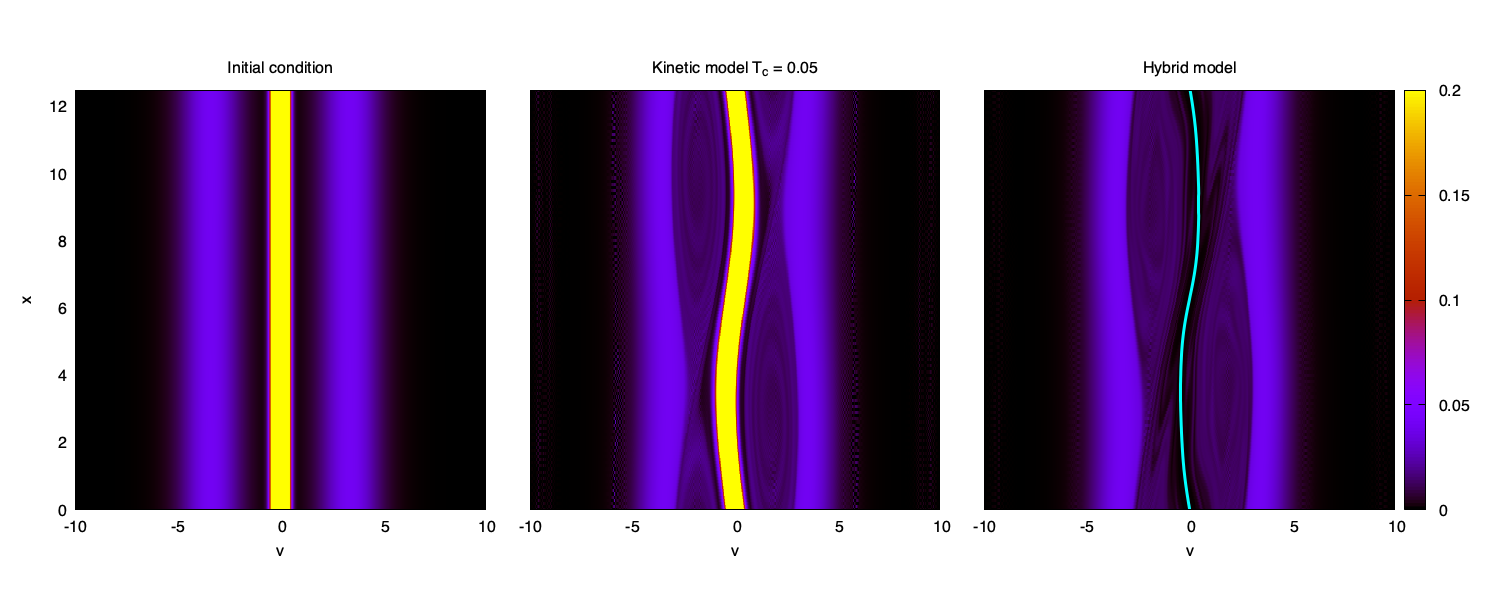
\includegraphics[width=\textwidth]{\localPath/figures/vp_t1.png}
  \caption{Représentation de la condition initiale du modèle cinétique à gauche et la solution obtenue au temps final $T_f=300$ avec le modèle cinétique avec $T_c = 0.05$ (au milieu) et la densité de particules chaudes obtenue avec modèle hybride linéarisé ainsi que la vitesse moyenne des particules froides (courbe cyan) (à droite).}
  \label{fig:limit_vp}
\end{figure}
\begin{figure}[h]
  \centering
  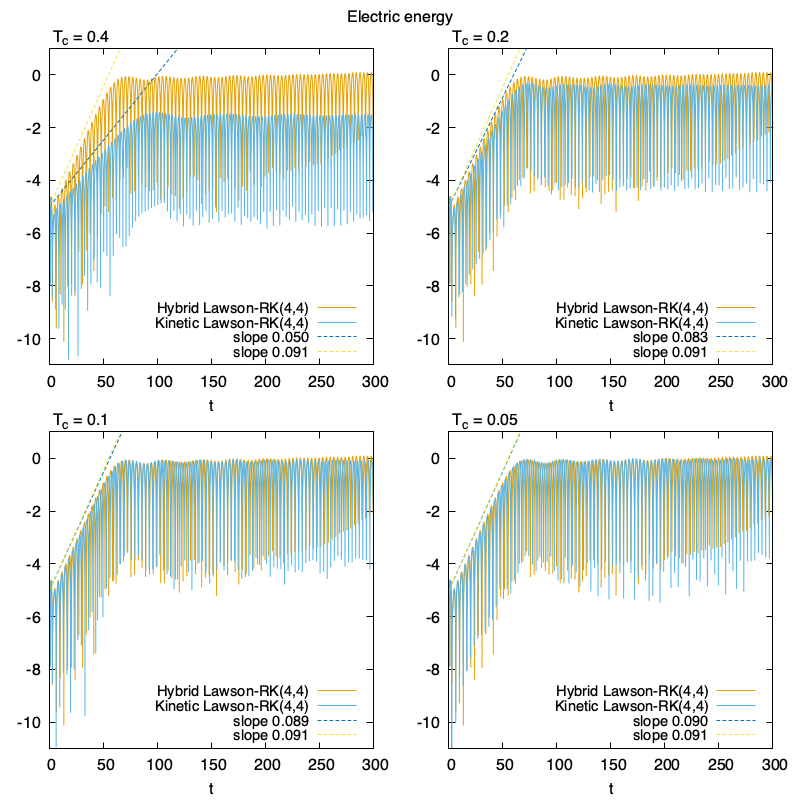
\includegraphics[width=\textwidth]{\localPath/figures/ee_t1.png}
  \caption{Énergie électrique donnée pour le modèle cinétique avec $T_c=0.05,0.1,0.2,0.4$ et le modèle hybride linéarisé.}
  \label{fig:limit_ee_Tf300}
\end{figure}
La première observation est que les résultats proches de ceux obtenus par le modèle hybride linéarisé \eqref{eq:vahl} sont très proches de ceux obtenus par le modèle cinétique \eqref{eq:vlasov}-\eqref{eq:poisson}, ce qui valide la modélisation. La perturbation des particules chaudes induit une instabilité (l'équilibre étant du type double gaussienne) qu'on voit se développer jusqu'au temps $t=75$ (voir figure \ref{fig:limit_ee_Tf300}), et deux vortex sont alors créés autour de la vitesse $v\approx 2$, au centre desquels de fines structures se développent. 

Dans la suite, nous allons approfondir cette étude en comparant les résultats obtenus aux relations de dispersion des deux modèles, puis en essayant de déterminer le domaine de validité du modèle VHL.  

%\commentaire[Anais]{(revoir un peu la rédaction de cette intro car elle ne tenait pas du tout compte de la sous-section relations de dispersion et je n'ai pas l'impression de l'avoir suffisamment modifiée)}

\FloatBarrier
%----------
\subsection{Convergence en énergie totale}
%----------

Nous nous intéresserons ici à une grandeur conservée qu'est l'énergie totale, celle-ci est la somme de l'énergie cinétique et de l'énergie électrique. Pour le modèle cinétique elle se calcule ainsi :
$$
  \mathcal{E}_K(t) = \iint_{\Omega\times\mathbb{R}} v^2 f\,\mathrm{d}x\mathrm{d}v + \int_{\Omega} E^2\,\mathrm{d}x. 
$$
Pour le modèle VHL, l'énergie cinétique comporte deux termes, un terme fluide pour les particules froides, et un terme cinétique pour les particules chaudes :
$$
  \mathcal{E}_{VHL}(t) = \int_\Omega \rho_c u_c^2\,\mathrm{d}x + \iint_{\Omega\times\mathbb{R}}v^2f_h\,\mathrm{d}x\mathrm{d}v + \int_\Omega E^2\,\mathrm{d}x
$$

\begin{pro}
  La différence en énergie totale entre le modèle cinétique et le modèle hybride linéarisé pour des conditions initiales données par~\eqref{eq:K:init} et~\eqref{eq:HL:init} converge en $(1-\alpha)T_c|\Omega|$.
\label{p:limit:convergence}
\end{pro}
\begin{proof}
  Pour le choix de $f^0$, l'énergie totale du modèle cinétique vaut :
  $$
    \begin{aligned}
      \mathcal{E}_K(t) = \mathcal{E}_K(0) &= \iint_{\Omega\times\mathbb{R}}v^2f^0(x,v)\,\mathrm{d}x\mathrm{d}v + \int_{\Omega}E^2(t=0,x)\,\mathrm{d}x \\
                                          &= \left[ (1-\alpha)T_c + \alpha v_0^2 + \alpha \right]|\Omega|
    \end{aligned}
  $$
    On remarque que lorsque $T_c\to 0$, on obtient $\lim_{T_c\to 0}\mathcal{E}_K(t) = (\alpha v_0^2 + \alpha)|\Omega|$. L'énergie totale dans le cadre du modèle hybride se calcule comme suit :
    $$
      \mathcal{E}_{HL}(t) = \int_\Omega \rho_c^{(0)}u_c^2\,\mathrm{d}x + \iint_{\Omega\times\mathbb{R}} v^2f_h\,\mathrm{d}x\mathrm{d}v + \int_\Omega E^2\,\mathrm{d}x
    $$
    ce qui nous donne, avec le choix de condition initiale $\rho_c^{(0)} = 1-\alpha$, $u_c^0 = 0$ et $f_h^0(v) = \mathcal{M}_{^\alpha/_2,v_0,1}(v) + \mathcal{M}_{^\alpha/_2,-v_0,1}(v)$, conformément à~\eqref{eq:HL:init} :
    $$
      \mathcal{E}_{HL}(t) = (\alpha v_0^2 + \alpha)|\Omega|
    $$
    qui est bien compatible avec $\lim_{T_c\to 0}\mathcal{E}_K(t)$. De plus on peut calculer :
    $$
      \mathcal{E}_K(t) - \mathcal{E}_{HL}(t) = (1-\alpha)T_c|\Omega|
    $$
    c'est-à-dire que la convergence du modèle hybride est liée à la pression $\rho_c^{(0)}T_c$ des particules froides.
\end{proof}

Pour vérifier numériquement cette proposition, nous effectuons un jeu de simulations. Le modèle cinétique de Vlasov-Poisson \eqref{eq:vlasov}-\eqref{eq:poisson} est simulé à l'aide d'une méthode en temps de type Lawson basée sur une méthode de Runge-Kutta d'ordre 4, la méthode WENO d'ordre 5 pour approcher la dérivée dans la direction $v$ et l'algorithme de FFT pour la dérivée dans la direction $x$. Il s'agit ainsi du même schéma que celui utilisé pour la fonction de distribution $f_h$ des particules chaudes du modèle hybride linéarisé. Nous choisissons la condition initiale \eqref{eq:K:init} avec $\alpha = 0.2$, $T_c \in \left\{ 0.05,0.1,0.2,0.4\right\}$, la discrétisation du domaine $\Omega = [0,4\pi]$ s'effectue avec $N_x = 135$ points, la discrétisation du domaine en vitesse $[-v_{\text{max}},v_{\text{max}}]$ nécessite de capturer la gaussienne représentant les particules froides pour différentes valeurs de $T_c$ ; nous choisissons donc d'adapter le nombre de points de discrétisation en vitesse $N_v$ à $T_c$, $N_v \in \left\{ 1431,1011,715,505 \right\}$, ceux-ci correspondant à une quinzaine de points de discrétisation pour capturer la gaussienne de température $T_c$. Nous avons une condition CFL sur le schéma WENO utilisé dans la direction $v$, nous nous assurons d'être sous cette condition quelle que soit l'évolution de $E$ en prenant $\Delta t = 0.5\Delta v$. Ce jeu de simulations s'arrête au temps 7, or le choix des différents $\Delta t$ implique des données à des temps différents ; nous choisissons d'effectuer une interpolation polynomiale de Lagrange d'ordre 5 pour exploiter les données au temps $T^\star = 6.5$. Nous obtenons ainsi l'énergie totale pour différentes températures sur la figure~\ref{fig:limit:totalenergy} ; bien que le schéma de type Runge-Kutta ne conserve pas exactement l'énergie, celle-ci est bien préservée en temps court et reste sous l'erreur machine en simple précision jusqu'au temps 50. Après l'interpolation au temps $T^\star = 6.5$ on obtient la convergence vers le modèle hybride sur la figure~\ref{fig:limit:totalenergy} (figure de droite) où l'on observe bien l'ordre 1 en température.
\begin{figure}[h]
  \centering
  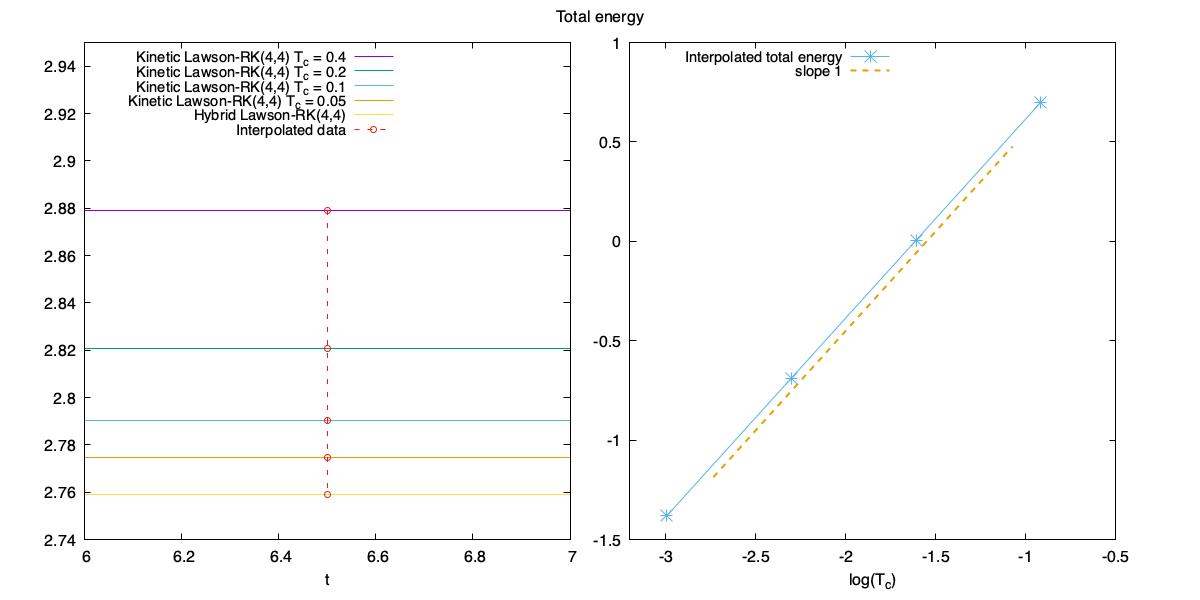
\includegraphics[width=\textwidth]{\localPath/figures/order_HTc.png}
  \caption{Énergie totale avec les différents modèles en échelle semi-log (gauche) et convergence de l'énergie totale du modèle cinétique vers le modèle hybride quand $T_c$ tend vers $0$ en échelle log (droite).}
  \label{fig:limit:totalenergy}
\end{figure}

Nous effectuons le même type d'analyse sur l'énergie électrique, à partir des données des simulations précédentes, en sachant que l'on n'a pas de résultat théorique sur sa convergence. L'énergie électrique pour les différents choix de $T_c$ est représentée sur la figure~\ref{fig:limit:ee} (gauche), cette figure illustre mieux la nécessité d'effectuer une interpolation pour extraire les données. Une convergence est observée sur la figure~\ref{fig:limit:ee} (droite).
\begin{figure}[h]
  \centering
  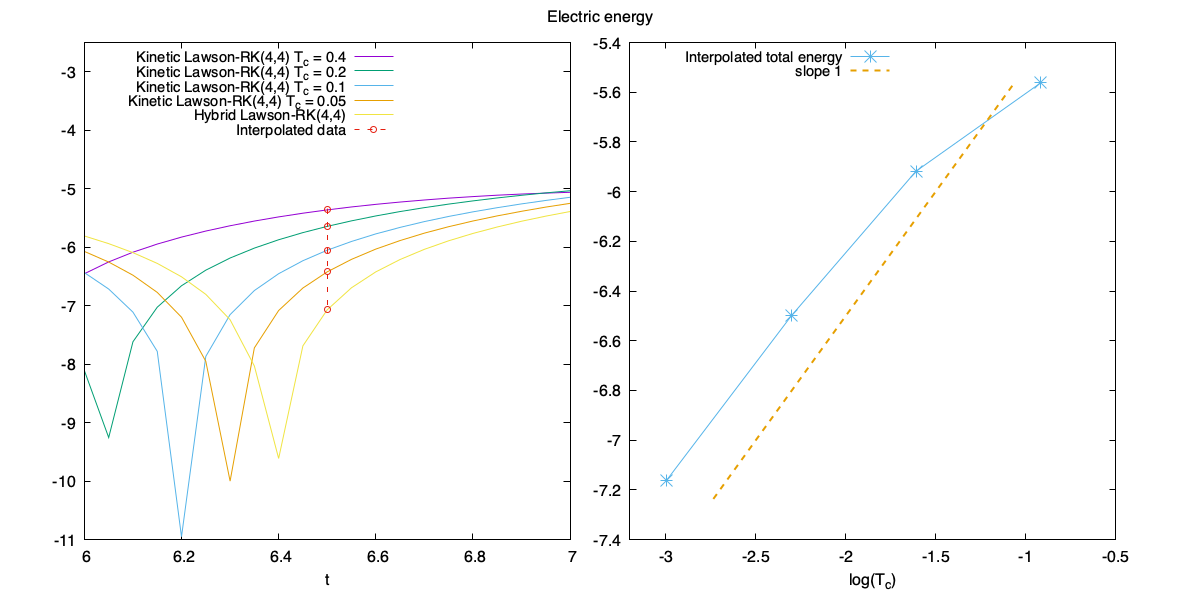
\includegraphics[width=\textwidth]{\localPath/figures/order_eeTc.png}
  \caption{Énergie électrique avec les différents modèles en échelle semi-log (gauche) et convergence de l'énergie totale du modèle cinétique vers le modèle hybride quand $T_c$ tend vers $0$ en échelle log (droite).}
  \label{fig:limit:ee}
\end{figure}

\FloatBarrier

%----------
\subsection{Convergence en température à l'aide des relations de dispersion}
%----------

Nous étudions numériquement la convergence des racines de la relation de dispersion quant $T_c$ tend vers $0$. Pour cela, on note $D^K_{[T_c]}(\omega,k)$ la relation de dispersion du modèle cinétique \eqref{D_3bump} et $D^H(\omega,k)$ la relation de dispersion du modèle VHL \eqref{eq:D_hchyb}. Pour $k$ fixé, on note $\omega\in\mathbb{C}$ la racine de plus grande partie imaginaire. 
%Pour la relation de dispersion, nous regardons les zéros en $\omega$ de la fonction $D^K_{[T_c]}(\omega,k)$ et $D^H(\omega,k)$ à $k$ fixé par la condition initiale. Nous ne conservons que le $\omega\in\mathbb{C}$ avec la plus grande partie imaginaire. 
Cette racine est calculée numériquement à l'aide d'une méthode de Newton. On étudie maintenant la convergence des $\omega_K$ (zéro de $(D^K(\omega,k)$) vers $\omega_H$ (zéro de $(D^H(\omega,k)$). La convergence de $\omega_K(T_c)$ vers $\omega_H$ est visible sur la figure \ref{fig:omega}, où l'on représente, en échelle log-log le module de la différence des deux zéros $\Delta \omega = |\omega_K-\omega_H|$.
\begin{figure}[h!]
  \centering
  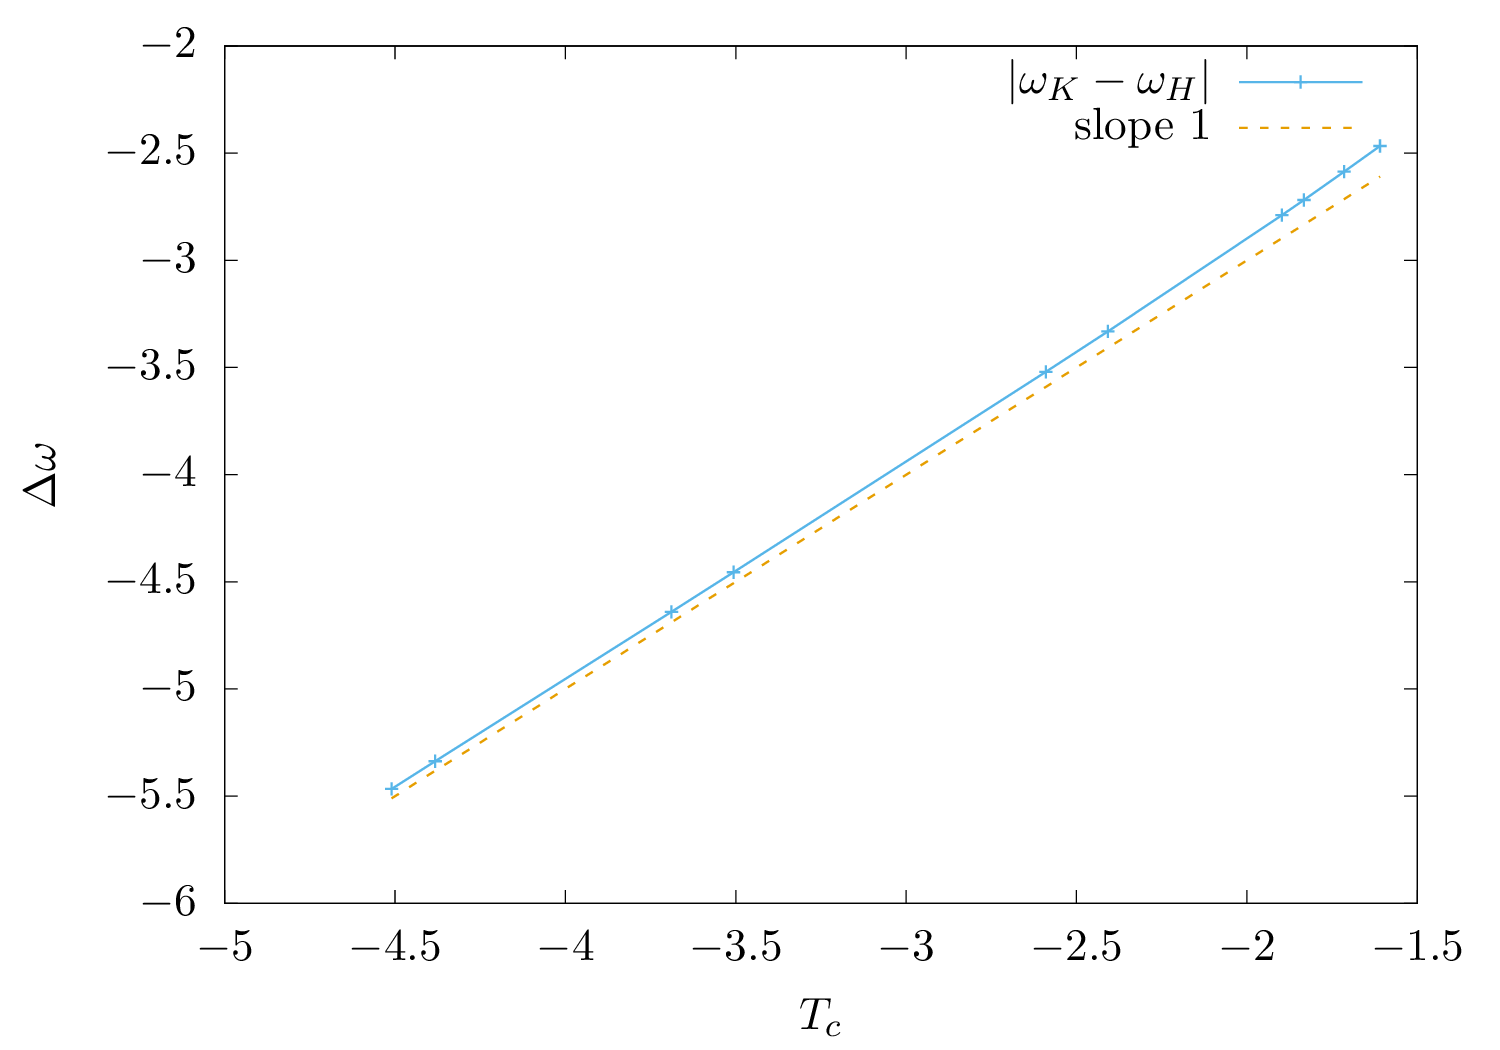
\includegraphics[width=0.8\textwidth]{\localPath/figures/omega.png}
  \caption{Convergence des zéros de la relation de dispersion cinétique vers la solution hybride}
  \label{fig:omega}
\end{figure}
On observe une convergence d'ordre $1$ en $T_c$ des zéros de la relation de dispersion, aucun argument théorique sur les fonctions holomorphes ne vient appuyer ce résultat, contrairement à ce qui a été énoncé pour l'énergie totale.

La racine de plus grande partie imaginaire permet de valider la phase linéaire du code. Cette phase linéaire peut être rendue plus longue en considérant une valeur très faible de la perturbation $\epsilon=10^{-4}$ dans les conditions initiales~\eqref{eq:K:init} et~\eqref{eq:HL:init}. Ceci va nous permettre de vérifier, non seulement le taux d'instabilité, mais aussi, grâce aux calculs de la section \ref{s:dispersion}, l'énergie électrique. Nous pouvons donc comparer pour $\alpha = 0.1$, $T_c=0.1$, $N_x=135$, $N_v=1200$, $T_f=200$ et $\Delta t = 0.5\Delta x$ ce régime linéaire sur la figure~\ref{fig:limit:ee:Tf200}\subref{fig:limit:ee:Tf200:eps10m4}. Un résultat similaire est observable pour différentes températures ainsi que sur le modèle hybride linéarisé, comme l'illustre la figure~\ref{fig:limit:ee:Tf200}\subref{fig:limit:ee:Tf200:cmp_zoom}. Les reconstructions de l'énergie électrique se font à partir des relations de dispersion, avec l'équation~\eqref{eq:enelec}.
\begin{figure}
  \centering
  \begin{subfigure}{0.8\textwidth}
    \centering
    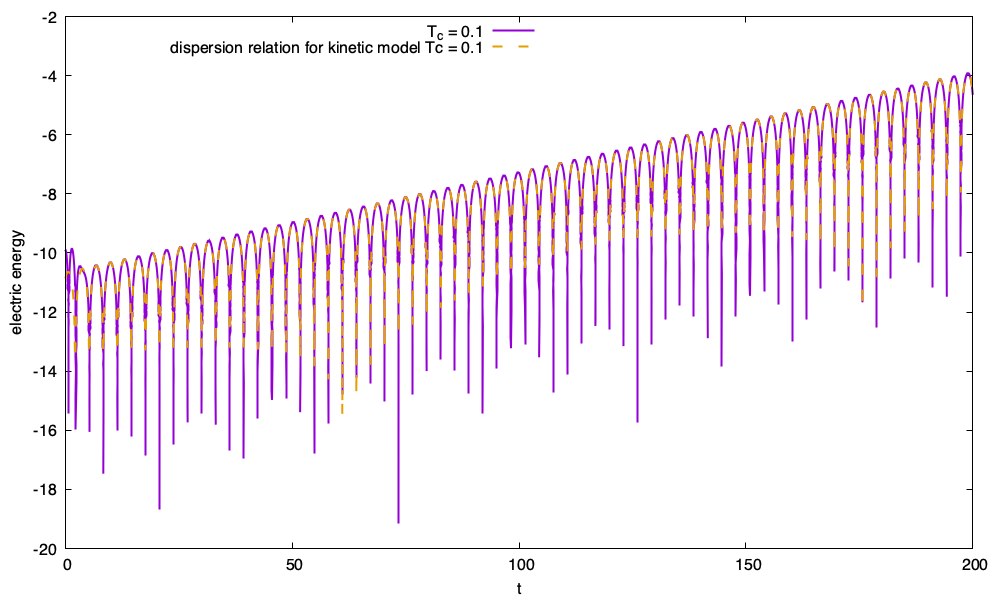
\includegraphics[width=\textwidth]{\localPath/figures/limit_ee_Tf200_eps10m4.png}
    \caption{Énergie électrique jusqu'au temps $200$ avec un régime linéaire très long, et comparaison avec les résultats données par les relations de dispersion.}
    \label{fig:limit:ee:Tf200:eps10m4}
  \end{subfigure}
  \begin{subfigure}{0.8\textwidth}
    \centering
    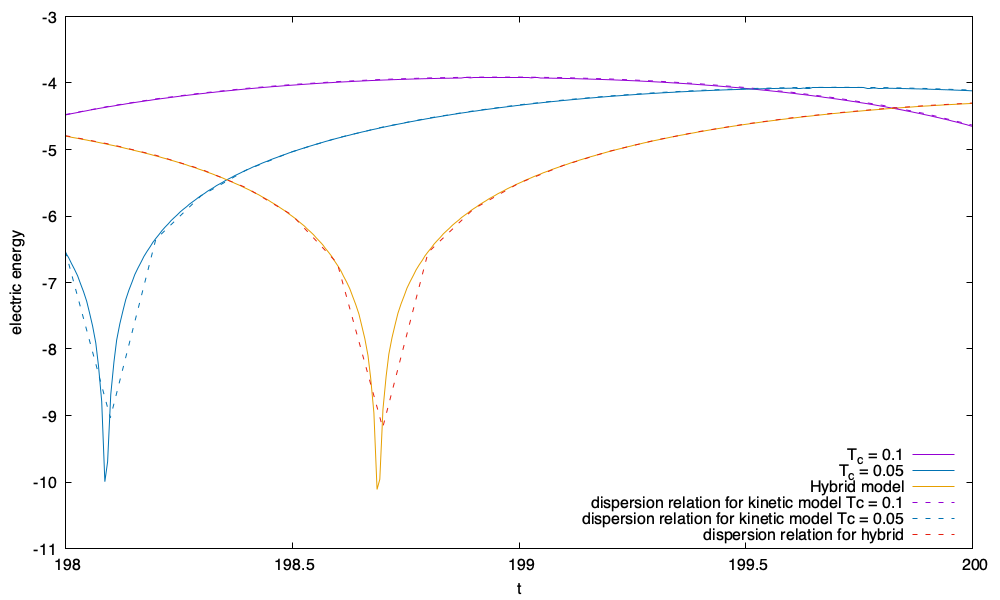
\includegraphics[width=\textwidth]{\localPath/figures/limit_ee_Tf200_cmp_zoom.png}
    \caption{Énergie électrique entre les temps $198$ et $200$ pour les températures $T_c = 0.1,0.05$ et le modèle hybride, et comparaison avec les résultats des relations de dispersion.}
    \label{fig:limit:ee:Tf200:cmp_zoom}
  \end{subfigure}
  \caption{Évolution de l'énergie électrique dans une longue phase linéaire et comparaison avec les relations de dispersion.}
  \label{fig:limit:ee:Tf200}
\end{figure}

En plus du taux d'instabilité de l'énergie électrique, il est possible, à l'aide des relations de dispersion, d'obtenir une très bonne approximation de l'énergie électrique dans la phase linéaire. On peut voir que l'étude des relations de dispersion ne permet pas d'obtenir des résultats fiables en début de simulation, où d'autres modes que le mode principal sont encore visibles (modes évanescents). De même, comme on peut le voir sur la figure~\ref{fig:limit_ee_Tf300}, la phase non-linéaire où l'énergie électrique atteint une saturation mélange de nombreux modes, ce qui est incompatible avec l'étude du linéarisé. Néanmoins, même au temps $t\approx 200$, les résultats du code sont en excellent accord avec ceux obtenus grâce aux relations de dispersion  (voir figure \ref{fig:limit:ee:Tf200:cmp_zoom}). 

\FloatBarrier
%----------
\subsection{Évolution avec la densité de particules chaudes}
%----------

Nous avons validé les modèles et les relations de dispersion lorsque la température des particules froides $T_c$ tend vers $0$ ; la proposition~\ref{p:limit:convergence} nous indique que la convergence s'effectue en $(1-\alpha)T_c|\Omega|$ où $\alpha$ est la densité des particules chaudes. Nous traçons sur la figure~\ref{fig:limit:slope:alpha} l'évolution du taux d'instabilité donné par les relations de dispersion (racine de plus grande partie imaginaire) en fonction de $\alpha$ et pour différentes valeurs de $T_c$. Cette évolution est représentée pour le modèle cinétique avec différentes températures, et  pour le modèle hybride, avec comme condition initiale pour les particules chaudes :
$$
  f_h^0(x,v) = \left(\mathcal{M}_{^\alpha/_2,4,1}(v) + \mathcal{M}_{^\alpha/_2,-4,1}(v)\right)(1+\epsilon\cos\left(k x\right)), \;\; x\in [0, 4\pi]. 
$$
La condition initiale du modèle cinétique est donnée par : $f^0(x,v) = \mathcal{M}_{1-\alpha,0,T_c}(v) + f_h^0(x,v)$.
\begin{figure}[h!]
  \centering
  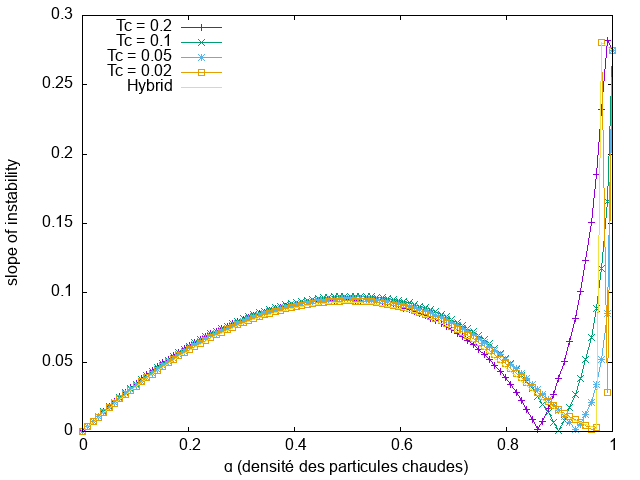
\includegraphics[width=0.8\textwidth]{\localPath/figures/limit_slope_alpha.png}
  \caption{Évolution de la pente du développement de l'instabilité (ou taux d'instabilité) donnée par les relations de dispersion en fonction de la densité de particules chaudes $\alpha$}
  \label{fig:limit:slope:alpha}
\end{figure}
On retrouve sur la figure~\ref{fig:limit:slope:alpha} la convergence en température du modèle cinétique vers le modèle hybride. Pour $\alpha=0$ la condition initiale se restreint aux particules froides, qui ne sont pas perturbées, il est donc normal d'obtenir une pente nulle ; pour $\alpha=1$, il n'y a que des particules chaudes et on retrouve l'instabilité double faisceau (TSI) avec le bon taux d'instabilité. On peut enfin observer que pour ce choix de $T_c$, les taux d'instabilité obtenus restent proches de ceux du modèle VHL pour $0\leq \alpha \leq 0.5$ (qui correspond à une population identique de particules chaudes et froides).

\FloatBarrier

%% section 6
% !TEX root = ../../main.tex

\section{Comparaison des deux résolutions hybrides}
\label{s:compare}

Dans cette section on s'intéressera à la comparaison des méthodes de simulation présentées dans la section~\ref{s:scheme} pour approcher numériquement le modèle VHL. On étudiera en particulier les méthodes de pas de temps adaptatif associées. Nous utilisons dans cette section la condition initiale suivante :
$$
  \begin{aligned}
    u_c(x)   &= 0 \\
    f_h(x,v) &=  \left(\mathcal{M}_{^\alpha/_2,v_0,1}(v) +  \mathcal{M}_{^\alpha/_2,-v_0,1}(v) \right)(1 + \epsilon\cos(kx))
  \end{aligned}
$$
avec $k=0.5$, $\alpha=0.2$, $v_0 = 3.4$, $x\in [0,L]$, $L=4\pi$, $v\in[-12,12]$, et la perturbation $\epsilon = 10^{-2}$. Le champ électrique initial $E(t=0,x)$ est obtenu en résolvant l'équation de Poisson sur notre condition initiale, comme indiqué dans la proposition~\ref{p:vhl_conservation}~:
$$
  \partial_x E(t=0) = (1-\alpha) + \int (1+\epsilon\cos(kx))\left( \mathcal{M}_{^\alpha/_2,v_0,1}(v) + \mathcal{M}_{^\alpha/_2,-v_0,1}(v) \right)\,\mathrm{d}v - 1
$$
La discrétisation du domaine s'effectue avec $N_x=27$ dans la direction $x$, et $N_v=128$ points dans la direction $v$.

Nous allons effectuer deux types de comparaisons entre les méthodes de \emph{splitting} hamiltonien et de Lawson. Une comparaison à pas de temps fixe, où on illustrera l'absence de condition de CFL des méthodes de \emph{splitting} ; puis une comparaison des méthodes de pas de temps adaptatif présentées dans la section~\ref{ssec:dtadapt} avec une tolérance $tol = 2\times10^{-5}$.

\subsection{Comparaison des deux résolutions hybrides à pas de temps fixe}

Cette section est dédiée à la comparaison entre la méthode de \emph{splitting} hamiltonien, présentée dans la sous-section~\ref{ssec:splitting}, et la méthode de Lawson présentée dans la sous-section~\ref{ssec:lawson}, pour la résolution du modèle hybride linéarisé~\eqref{eq:vahl}.

Nous considèrerons trois pas de temps différents :
\begin{itemize}
  \item $\Delta t = 0.1 \approx 0.5\Delta v$, il s'agit d'une condition de CFL classique pour des méthodes de volumes finis ;
  \item $\Delta t = 0.5 \approx \sigma\frac{\Delta v}{\|E^n\|_\infty} = 0.54$, with $\sigma\approx 1.732$, il s'agit de la condition de CFL entre WENO5 et RK($4$,$4$) calculé dans le chapitre précédent ou~\cite{Crouseilles:2019b}, et calculé à partir d'une précédente estimation numérique $\|E^n\|_\infty = \max_{i,n}|E^n_i|\approx 0.6$ ;
  \item $\Delta t = 0.7$, il s'agit dans ce cas d'un cas test avec un pas de temps plus grand que la CFL de la méthode de Lawson, pour illustrer que la méthode de \emph{splitting} n'a pas de contrainte de stabilité sur le pas de temps.
\end{itemize}

Sur la figure~\ref{fig:compare:ee}, on trace l'évolution de l'énergie électrique (en échelle semi-log) calculée par deux méthodes d'ordre 4 (méthode de Suzuki et de Lawson-RK(4,4)), avec différentes valeurs de pas de temps $\Delta t$, $0.1$, $0.5$ et $0.7$. On note que toutes les simulations capturent correctement l'énergie électrique dans la phase linéaire, jusqu'au temps 60, même lorsque la méthode est instable. Pour $\Delta t=0.1,0.5$, on vérifie la stabilité prévue des méthodes, qui donnent des résultats très similaires. Dans le cas $\Delta t=0.7$, la méthode de Lawson-RK(4,4) devient instable dans la phase non-linéaire, c'est en fait dans cette phase que l'amplitude du champ électrique atteint son maximum, et le paramètre $\Delta t=0.7$ viole la condition de CFL, alors que la méthode de \emph{splitting} de Suzuki reste stable comme prévu.

\begin{figure}[h]
  \centering
  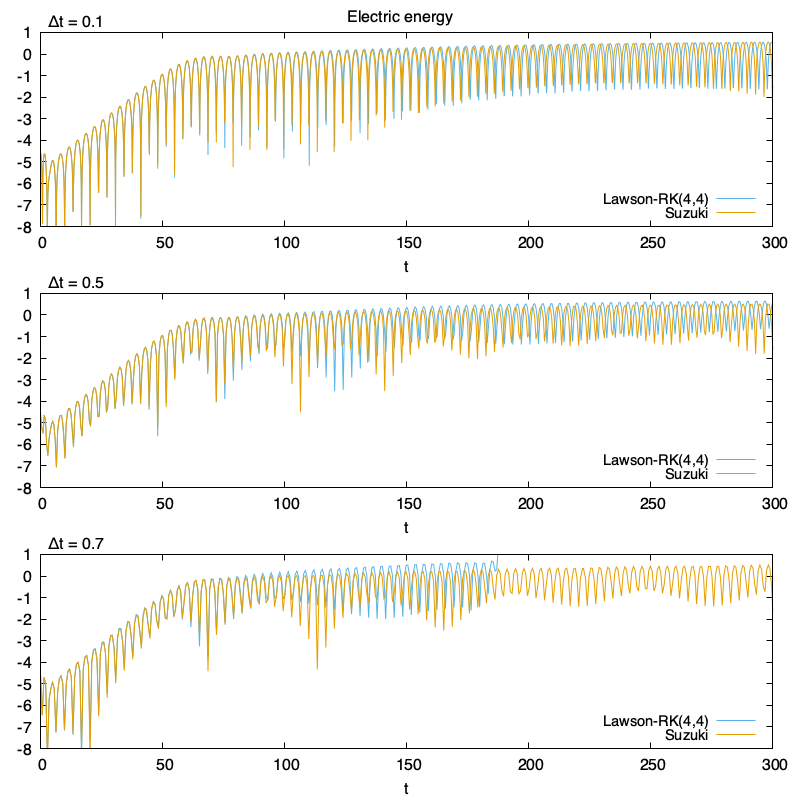
\includegraphics[width=\textwidth]{\localPath/figures/ee_t2.png}
  \caption{Évolution de l'énergie électrique pour le modèle hybride (résolu avec la méthode de Lawson et de Suzuki) pour différentes valeurs de pas de temps $\Delta t=0.1,0.5,0.7$.}
  \label{fig:compare:ee}
\end{figure}


Sur la figure~\ref{fig:H:t2}, on observe l'évolution de l'erreur relative sur l'énergie totale, calculée par :
\begin{equation}
	\frac{\mathcal{H}^n}{\mathcal{H}^0}-1
	\label{eq:relativeerror:H}
\end{equation}
avec :
$$
  \mathcal{H}^n = \frac{1}{2}\iint v^2f_h^n\dd{v}\dd{x}
                + \frac{1}{2}\int\rho_c^{(0)}\left(u_c^n\right)^2\dd{x}
                + \frac{1}{2}\int\left(E^n\right)^2\dd{x}.
$$
On considère les mêmes paramètres numériques et on compare l'effet de la méthode d'intégration en temps (méthode de \emph{splitting} hamiltonien : Lie~\eqref{eq:lie}, Strang~\eqref{eq:strang} et Suzuki~\eqref{eq:suzuki}, et la méthode Lawson-RK(4,4)) sur la préservation de l'énergie totale. On observe que les méthodes géométriques de \emph{splitting} hamiltonien préservent très bien l'énergie totale, en particulier, l'erreur relative oscille autour d'une constante en temps long, ce qui est un comportement typique d'une méthode géométrique. On observe que la méthode de Lawson, si le pas de temps est pris sous la condition de CFL, l'erreur est proche de $4\%$, ce qui est acceptable. Évidemment, comme évoqué précédemment sur l'énergie électrique, on observe un problème lorsque $\Delta t=0.7$, l'erreur donnée par la méthode Lawson-RK($4$,$4$) diverge dans la phase non-linéaire, à cause de l'instabilité numérique ; avant cela, l'erreur est autour des $2\%$. Le tableau~\ref{tab:H:max} résume le maximum de l'erreur relative $\max_n \left| {\cal H}^n / {\cal H}^0 -1 \right|$ pour les différentes méthodes et les différents pas de temps considérés.

\begin{figure}[h]
  \centering
  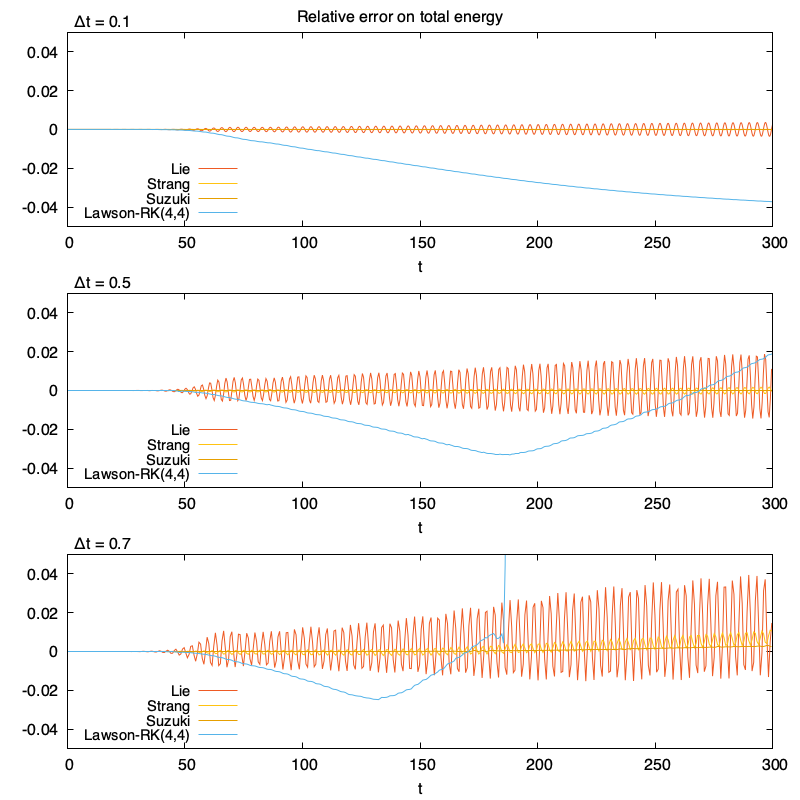
\includegraphics[width=\textwidth]{\localPath/figures/H_t2.png}
  \caption{Évolution de l'erreur relative sur l'énergie totale pour le modèle hybride (résolu avec la méthode de Lawson et de Suzuki) pour différentes valeurs de pas de temps $\Delta t=0.1,0.5,0.7$.}
  \label{fig:H:t2}
\end{figure}

\begin{table}[h]
  \centering
  \begin{tabular}{l|c|c|c}
                   & $0.1$             & $0.5$     & $0.7$        \\
    \hline
    Lie            & $0.0036$          & $0.0187$  & $0.0394$     \\
    Strang         & $0.0001$          & $0.0019$  & $0.0109$     \\
    Suzuki         & $3\times 10^{-8}$ & $0.0001$  & $0.0028$     \\
    Lawson-RK(4,4) & $0.0372$          & $0.0331$  & \texttt{NaN} \\
  \end{tabular}
  \caption{Maximum de l'erreur relative donnée sur la figure~\ref{fig:H:t2}.}
  \label{tab:H:max}
\end{table}

Dans le cas $\Delta t=0.1$, on compare sur la figure~\ref{fig:vp:t2} la distribution de particules chaudes $f_h$ calculée par les méthodes de Suzuki et de Lawson-RK(4,4) au temps $t=100$, sur laquelle on ajoute la vitesse moyenne des particules froides $u_c$. Les solutions numériques ainsi obtenues sont très proches, la position des vortex et l'allure de la vitesse moyenne des particules froides sont très similaires entre les deux méthodes. On observe aussi que la méthode Lawson-RK(4,4) introduit plus de diffusion numérique que la méthode de Suzuki, en effet les vortex semblent avoir une meilleure résolution. Cela peut s'expliquer par la discrétisation dans l'espace des phases dans la direction $v$, une méthode WENO5 (avec limiteurs de pente) est utilisé avec la méthode Lawson-RK(4,4), contre une interpolation d'ordre 5 par des polynômes de Lagrange (sans limiteurs de pente) avec la méthode de Suzuki.

\begin{figure}[h]
  \centering
  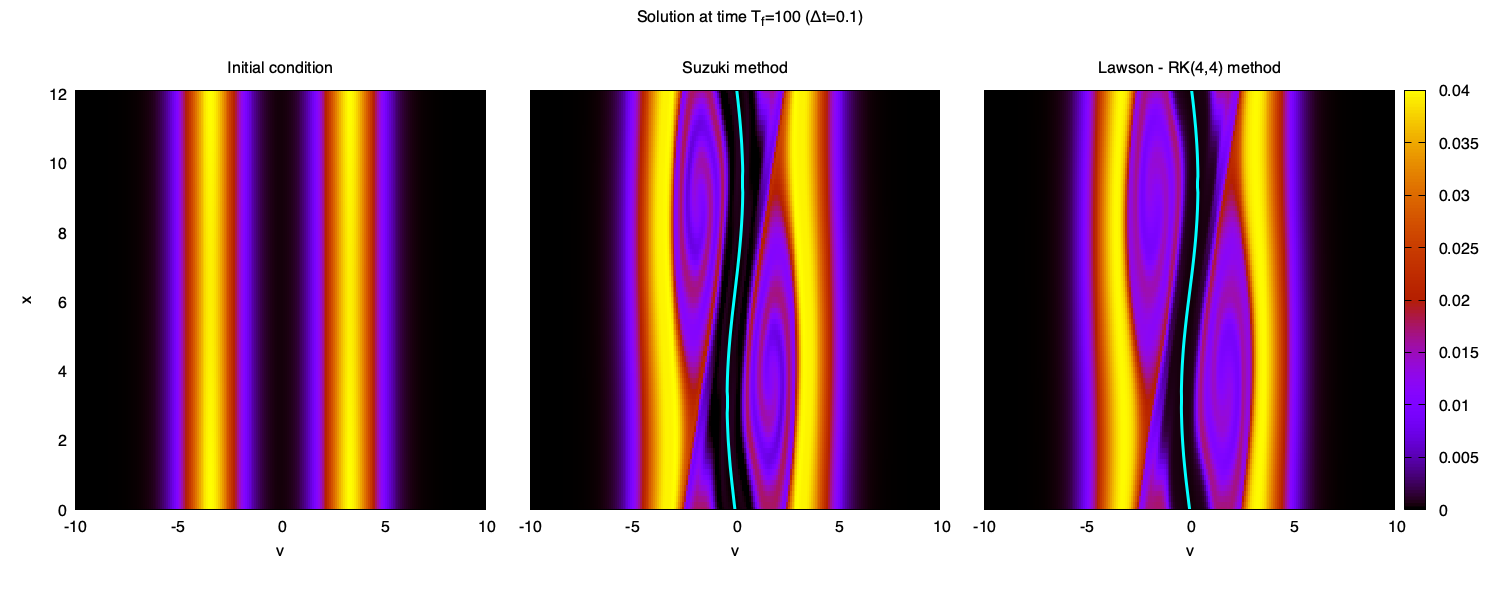
\includegraphics[width=0.9\textwidth]{\localPath/figures/vp_t2.png}
  \caption{Densité des particules chaudes $f_h$ et vitesse moyenne des particules froides $u_c$ (en cyan) la condition initiale (gauche), au temps $t=100$ calculée par la méthode de Suzuki (milieu) et calculée par la méthode de Lawson-RK(4,4) (droite).}
  \label{fig:vp:t2}
\end{figure}

\begin{figure}
	\centering
	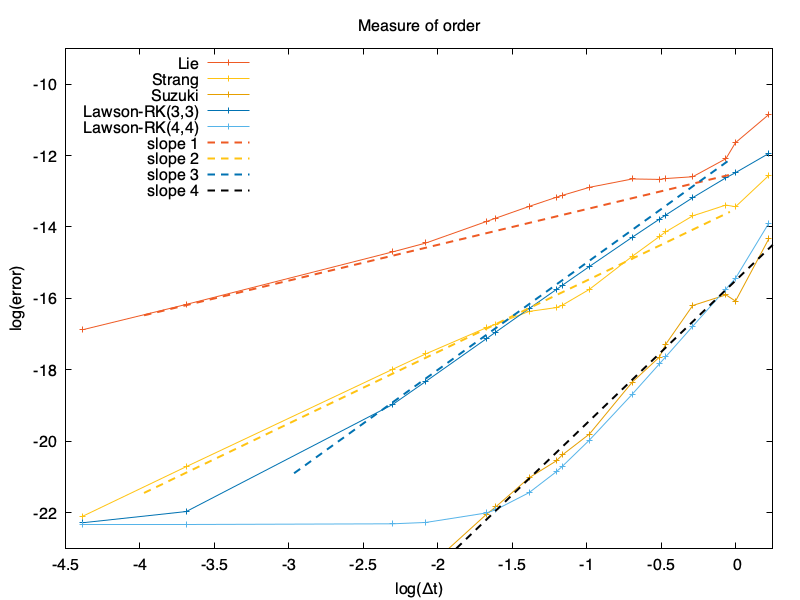
\includegraphics[width=0.75\textwidth]{\localPath/figures/order_t2.png}
	\caption{Étude de l'ordre en temps des différentes méthodes numériques pour résoudre le modèle hybride (méthodes de Lawson et de \emph{splitting}). L'erreur est calculée à partir du maximum de l'erreur relative sur l'énergie totale.}
	\label{fig:order:t2}
\end{figure}

Pour compléter cette étude, on trace sur la figure~\ref{fig:order:t2} l'ordre en temps des différents intégrateurs en temps utilisés pour résoudre le modèle hybride : les méthodes de \emph{splitting} hamiltonien (Lie, Strang et Suzuki), les méthodes de Lawson (RK(4,4) et RK(3,3)). Pour cela on calcule le maximum de l'erreur relative sur l'énergie totale : $\max_n|\mathcal{H}^n/\mathcal{H}^0-1|$, jusqu'au temps $t=15$, en fonction du pas de temps $\Delta t\in[0.01,0.125]$, avec $N_x=243$ et $N_v=512$. Tous les ordres théoriques des méthodes en temps sont bien reconstruits. On remarque que la constante d'erreur entre la méthode de Suzuki et de Lawson-RK(4,4) sont très proches, mais que cette première est légèrement plus coûteuse que la méthode de Lawson (plus de détails dans la section~\ref{ssec:2:time}).

\FloatBarrier

\subsection{Comparaison des deux méthodes de pas de temps adaptatif}
\label{ssec:2:dtn}

Cette section est dédiée à l'étude des méthodes de Suzuki et de Lawson avec leur stratégie de pas de temps adaptatif associée, présentée dans la section~\ref{ssec:dtadapt}. Pour toutes les simulations nous nous somme intéressés à l'estimateur d'erreur qui dans ce cas s'écrit :
\begin{equation}
  \begin{aligned}
    L^{n+1}_{[3]} & = \left(\sum_{i=0}^{N_x-1}\left( {u_c}_i^{n_1,[4]}-{u_c}_i^{n_1,[3]} \right)^2\Delta x\right)^{\frac{1}{2}}
                    + \left(\sum_{i=0}^{N_x-1}\left( {E}_i^{n_1,[4]}-{E}_i^{n_1,[3]} \right)^2\Delta x\right)^{\frac{1}{2}} \\
                  & + \left(\sum_{i=0}^{N_x-1}\sum_{j=0}^{N_v-1}\left| {f_h}_{i,j}^{n_1,[4]}-{f_h}_{i,j}^{n_1,[3]} \right|^2\Delta v\Delta x\right)^{\frac{1}{2}} \\
                  & = L_{u_c}^{n+1} + L_{E}^{n+1} + L_{f_h}^{n+1},
  \end{aligned}
  \label{eq:LucEfh:localerror}
\end{equation}
où ${u_c}_i^{n+1,[p]}$,${E}_i^{n+1,[p]}$ et ${f_h}_{i,j}^{n+1,[p]}$ sont les inconnues discrétisées calculées avec une méthode d'ordre $p$ en temps et associées au temps $t^{n+1}$ et au point $x_i=i\Delta x$, $i=0,\dots,N_x$ et $v_j = -v_\text{max} + j\Delta v$, $j=0,\dots,N_v$ de l'espace des phases. Pour les deux méthodes, si le critère d'erreur $\|L_{[3]}^{n+1}\|<tol$ est satisfait, alors l'itération est acceptée et le temps incrémenté, sinon l'itération est rejetée et reprend au temps $t^n$. Dans les deux cas, le pas de temps suivant est calculé en utilisant~\eqref{eq:dtopt}. Cela nous permet de comparer l'estimateur d'erreur avec la même tolérance $tol$ (prise arbitrairement à $tol=2\times10^{-5}$) entre les deux intégrateurs en temps : la méthode de Suzuki et DP4(3). Nous regarderons aussi la taille des pas de temps proposés par les deux méthodes et le nombre d'itérations nécessaires pour finir la simulation.

\begin{table}[h]
	\centering
	\begin{tabular}{c|c|c|c}
      méthode             & nombre d'itérations & nombre d'itérations acceptées & ratio \\
%      \hline
%       $\Delta t = 0.5$ & 600                  & 600                          & 1     \\
%       $\Delta t = 0.1$ & 3000                 & 3000                         & 1     \\
      \hline
      Suzuki              & 23895                & 23849                        & 0.998 \\
      Lawson-DP4(3)       & 2288                 & 2192                         & 0.958 \\
	\end{tabular}
	\caption{Comparaison du nombre d'itérations pour résoudre le problème jusqu'au temps $t=300$, le nombre d'itérations acceptées de la méthode de pas de temps adaptatif et le ratio entre le nombre d'itérations acceptées et le nombre total d'itérations.}
	\label{tab:compare:iteration}
\end{table}

Le tableau~\ref{tab:compare:iteration} présente le nombre d'itérations nécessaires pour atteindre le temps final $t=300$ pour les deux méthodes de pas de temps adaptatif considérées (méthode de Suzuki et de Lawson-DP4(3)) avec les paramètres numériques suivants $N_x=81$, $N_v=128$. Le nombre d'itérations acceptées (itérations où le critère d'erreur $\|L_{[3]}^{n+1}\|<tol$ est satisfait), et le ratio entre le nombre d'itérations acceptées et le nombre total d'itérations est aussi présenté. On observe qu'une très large majorité des itérations sont acceptées pour les deux méthodes, ce qui signifie que l'estimateur d'erreur est un bon indicateur. Pour la méthode de Lawson-DP4(3) le ratio d'itérations acceptées est légèrement plus faible que pour la méthode de Suzuki, ce qui signifie que la stratégie de pas de temps adaptatif essaie des pas de temps plus larges qui sont parfois rejetés. La très faible proportion d'itérations rejetées indique qu'il est très rarement nécessaire de recalculer une itération avec un pas de temps plus petit. Le surcoût engendré par la méthode de pas de temps adaptatif est donc négligeable. La seconde remarque que l'on peut faire est à propos de la méthode de Suzuki, qui nécessite 10 fois plus d'itérations que la méthode de Lawson-DP4(3) pour atteindre le temps final $t=300$, ce qui signifie que la méthode de Suzuki nécessite de plus petits pas de temps pour satisfaire le critère d'erreur $\|L_{[3]}^{n+1}\|<tol$.

Sur la figure~\ref{fig:compare:dt_and_error} est représentée l'évolution de la taille du pas de temps au cours du temps, en effet celui-ci suit l'équation~\eqref{eq:dtopt} et est donc recalculé à chaque itération. Les itérations rejetées, celles où le critère d'erreur n'est pas satisfait, sont représentées avec des carrés. On remarque tout d'abord que dans la phase linéaire (jusqu'au temps $t\approx 50$) des pas de temps plus grands sont pris. Pendant la phase non-linéaire, le pas de temps oscille près d'une constante, qui permet de capturer les effets non-linéaires (vortex dans la distribution de particules) et les forts gradients (filamentation issue de la formation des votex). On remarque ensuite, que pour une même tolérance ($tol=2\times10^{-5}$), la méthode de Suzuki nécessite de plus petits pas de temps, comparé à la méthode DP4(3), pour satisfaire le critère d'erreur, comme remarqué dans le tableau~\ref{tab:compare:iteration}. On remarque que les variations du pas de temps sont relativement importantes ; il est possible de contrôler ces oscillations en limitant l'évolution des pas de temps en prenant par exemple $\Delta t^{n+1}\in[0.5\Delta t^n,2\Delta t^n]$, comme proposé dans \cite{Balac:2014}. Sur la figure~\ref{fig:compare:error:dtc} est tracée l'évolution de l'erreur locale $L_{[3]}^n$ comme une fonction du temps pour la méthode de Lawson (gauche) et de Suzuki (droite), avec une stratégie de pas de temps adaptatif et une stratégie de pas de temps constant. Pour un grand pas de temps ($\Delta t = 0.5$), les méthodes sont stables, mais le pas de temps dépasse largement la tolérance fixée à $tol=2\times10^{-5}$. Les méthodes à pas de temps adaptatif, choisissent automatiquement un pas de temps permettant de garantir une erreur locale sous la tolérance. La méthode de Lawson avec un pas de temps adaptatif (DP4(3)) et avec un pas de temps fixe à $\Delta t = 0.1$ (RK(4,4)) calculent une erreur locale très proche, pourtant la méthode DP4(3) optimise son pas de temps pour assurer une erreur locale sous la tolérance, et permet d'obtenir des pas de temps plus grand que $\Delta t =0.1$ comme on peut le remarquer sur la figure~\ref{fig:compare:dt_and_error}. Assurer une erreur sous une tolérance avec les plus grands pas de temps possible est une heuristique intéressante. En ce qui concerne les résultats avec la méthode de Suzuki, on remarque de nouveau que la stratégie requière de plus petits pas de temps, comparé à DP4(3), pour assurer une estimation de l'erreur locale sous la tolérance. De plus, avec un pas de temps constant à $\Delta t = 0.1$, la méthode de Suzuki génère des erreurs locales bien plus importantes, alors que la méthode DP4(3) était presque sous la tolérance.

\begin{figure}[h]
  \centering
  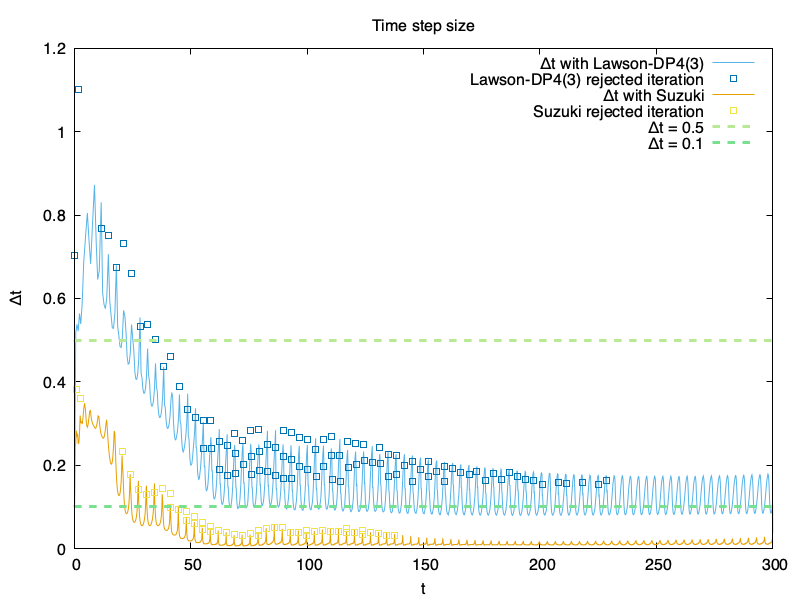
\includegraphics[width=0.75\textwidth]{\localPath/figures/dt_size_t3.png}
  \caption{Évolution du pas de temps $\Delta t_n$ (les itérations rejetées sont représentées par des carrés) pour la modèle hybride avec des méthodes de pas de temps adaptatif.} 
  \label{fig:compare:dt_and_error}
\end{figure}

\begin{figure}[h]
  \centering
  \includegraphics[width=0.49\textwidth]{\localPath/figures/Ll_t3.png}
  \includegraphics[width=0.49\textwidth]{\localPath/figures/Ls_t3.png}
  \caption{Comparaison de l'évolution en temps de l'estimateur d'erreur pour une méthode à pas de temps constant et à pas de temps adaptatif. La méthode de Lawson est à gauche. La méthode de Suzuki est à droite. Les résultats sont en échelle semi-$\log$.}
  \label{fig:compare:error:dtc}
\end{figure}
\begin{figure}[h]
  \centering
  \includegraphics[width=0.8\textwidth]{\localPath/figures/L_LucEfh_t3.png}
  \caption{Comparaison de la contribution de chaque composante de l'estimateur d'erreur locale en fonction du temps, pour la méthode de Lawson (haut) et de Suzuki (bas).}
  \label{fig:compare:error:LucEfh}
\end{figure}

Pour les deux méthodes à pas de temps adaptatif, on s'intéresse maintenant à l'évolution de l'estimateur d'erreur locale au cours du temps, en prennant en compte les différentes contributions de $L^n_{[3]}$, à savoir $L^n_{u_c}$, $L^n_{E}$ et $L^n_{f_h}$ définies dans~\eqref{eq:LucEfh:localerror}. Les résultats sont visibles sur la figure~\ref{fig:compare:error:LucEfh}. L'erreur de la méthode DP4(3) et de ces différentes contributions sont visibles en haut, alors que celles de la méthode de Suzuki sont tracées en bas. Pour la méthode DP4(3), on remarque tout d'abord que la contribution venant de $L^n_{u_c}$ est négligeable (autour de l'erreur machine), ce qui peut s'expliquer par le fait que dans la méthode de Lawson la partie linéaire est résolue exactement. Puisque la partie non-linéaire de la méthode de Lawson comprend le calcul du courant chaud $\int vf_h\dd{v}$ qui va impacter $L^n_E$ et le transport dans la direction $v$ qui va impacter $L^n_{f_h}$, les contributions à l'estimateur d'erreur de ces deux contributions restent prépondérantes tout au long de la simulation. Pour la méthode de Suzuki, l'erreur provient essentiellement de $L^n_{f_h}$, erreur venant de l'interpolation du transport dans la direction $v$. Il est à noter, que les erreurs $L^n_{u_c}$, $L^n_{E}$ ne sont pas nulles au delà du temps $t\approx 50$, mais sont respectivement de l'ordre de $10^{-10}$ et $10^{-8}$.

%\FloatBarrier

\subsection{À propos des temps de calcul}
\label{ssec:2:time}

Pour finir la comparaison entre les méthodes de \emph{splitting} et de Lawson, nous comparerons leurs temps de calcul. Sur la figure~\ref{fig:timer_boxplot_t4} (gauche), on représente la valeur moyenne ainsi que les quartiles du temps de calcul d'une itération de RK(4,4), DP4(3) et de la méthode de Suzuki. Nous rappelons que la méthode RK(4,4) est constituée de 4 étages, alors que les méthodes DP4(3) et de Suzuki en comprennent 5. Cela explique pourquoi une itération de la méthode RK(4,4) coûte moins qu'une itération des deux autres méthodes. Sur la partie de droite de la figure~\ref{fig:timer_boxplot_t4} on compare le temps de calcul de chaque étape des différentes méthodes. On rappelle que la méthode DP4(3) est formée à partir des 4 étages de la méthode RK(4,4) plus un étage supplémentaire. Comme espéré, chaque étape de la méthode de Suzuki a le même coût (puisque la méthode de Suzuki est une composition de 5 méthode de Strang). Au contraire, on observe que les deux premiers étages des méthodes RK(4,4) ou DP4(3) sont moins coûteux que les autres étages, ces deux premiers contenant moins d'opérations.

\begin{figure}[h]
  \centering
  \includegraphics[width=\textwidth]{\localPath/figures/timer_boxplot_t4.png}
  \caption{Valeur moyenne et quartiles du temps de calcul sur une itération (gauche) et pour chaque étape d'une itération (droite).}
  \label{fig:timer_boxplot_t4}
\end{figure}

%% section 7
% !TEX root = ../../main.tex

\section{Conclusion}
% -------------------------------------------------------------------

Au cours de ce chapitre nous avons pu étudier et confirmer numériquement la convergence du modèle cinétique $1dx-1dv$ vers le modèle hybride. Nous avons décrit deux méthodes de résolution du modèle hybride. La première méthode, méthode de \emph{splitting}, tirant parti de la structure hamiltonienne du système et assurant le bon comportement en temps long de certaines quantités (énergie, masse). La seconde méthode de résolution est basée sur une méthode de Lawson, et ne préserve aucune quantité particulière, mais permet une montée en ordre en temps pour un coup numérique plus faible. La comparaison des résultats s'est faite grâce à une étude fine des relations de dispersion, permettant de reconstruire le champ électrique et de déterminer le taux d'instabilité dans nos cas tests.

Un résultat supplémentaire que nous avons pu obtenir dans cette comparaison, est l'intérêt plus important de la méthode de pas de temps adaptatif basée sur la méthode de Lawson, permettant de profiter de toute la littérature sur les méthodes de type Runge-Kutta.

En perspective, il est possible d'étudier le modèle hybride, en tenant compte des termes non-linéaires dans la partie fluide. Dans un contexte plus perturbatif, il est possible que ceux-ci capturent mieux la solution du modèle cinétique, cadre où les hypothèse de linéarisation sont violées. 

Différentes perspectives sont en cours d'étude en ce qui concerne la résolution numérique. Il est envisageable d'augmenter la partie linéaire de l'équation de Vlasov-Ampère hybride linéarisé~\eqref{eq:vahl} en y intégrant le calcul du courant, en effet le système devient, après une transformée de Fourier en $x$, pour un mode de Fourier $\kappa$ :
$$
  \begin{cases}
    \partial_t\hat{f}_{h,\kappa} + i\kappa v\hat{f}_{h,\kappa} + \widehat{\left(E\partial_vf_h\right)}_\kappa = 0 \\
    \partial_t \hat{u}_{c,\kappa} = \hat{E}_\kappa \\
    \partial_t\hat{E}_\kappa = -\rho_c^{(0)}\hat{u}_{c,\kappa} -\int_\mathbb{R} v\hat{f}_{h,\kappa}\dd{v}.
  \end{cases}
$$
En discrétisant en $v$ le problème, et en calculant le courant induit par les particules chaudes $j_h$ à l'aide de la méthode des rectangles :
$$
  \int_\mathbb{R} v\hat{f}_{h,\kappa}\dd{v} = \hat{j}_h \approx \sum_{j=1}^{N_v} v_j\hat{f}_j\Delta v
$$
avec $v_j = -v_{\text{max}}+ j\Delta v$, il est possible de réécrire le problème comme :
$$
  \partial_t \begin{pmatrix}
    \hat{f}_{h,\kappa,1} \\
    \vdots \\
    \hat{f}_{h,\kappa,N_v} \\
    \hat{u}_{c,\kappa} \\
    \hat{E}_\kappa
  \end{pmatrix}
  =
  \begin{pmatrix}
    \mqty{
      \mqty{
        \mqty{\dmat{-i\kappa v_1,\ddots,-i\kappa v_{N_v}}} \\
        \mqty{0            &\cdots& 0               \\
              -v_1\Delta v &\cdots& -v_{N_v}\Delta v }
      }
      &
      \mqty{
        0             & 0      \\
        \vdots        & \vdots \\
        0             & 0      \\
        0             & 1      \\
        -\rho_c^{(0)} & 0
      }
    }
  \end{pmatrix}
  \begin{pmatrix}
    \hat{f}_{\kappa,1} \\
    \vdots \\
    \hat{f}_{\kappa,N_v} \\
    \hat{u}_{c,\kappa} \\
    \hat{E}_\kappa
  \end{pmatrix}
  +
  \begin{pmatrix}
    -\widehat{(E\partial_vf)}_{\kappa,1} \\
    \vdots \\
    -\widehat{(E\partial_vf)}_{\kappa,N_v} \\
    0 \\
    0
  \end{pmatrix}.
$$
Ceci s'applique également au modèle de Vlasov-Ampère~\eqref{eq:vlasov}-\eqref{eq:ampere}. Cette stratégie permet de garantir que l'équation de Poisson sous-jacente est satisfaite. De plus les contributions des estimateurs d'erreur $L_{u_c}$ et $L_E$ passent sous l'erreur machine car mettant en jeu que des variables résolues dans la partie linéaire (et donc exacte), dans le cadre d'une méthode à pas de temps adaptatif, comme présentée sur la figure~\ref{fig:compare:error:LucEfh}.

La résolution de ce problème avec une méthode de Lawson, permet d'envisager l'utilisation de méthodes de Lawson semi-implicites, permettant de lever des conditions de stabilité en $v$. Pour cela il est possible de construire des méthodes de Lawson induites par une méthode DIRK (\emph{Diagonally Implicit Runge-Kutta}), famille de méthodes présentée dans~\cite{Alexander:1976}, une autre stratégie est l'utilisation de méthodes IMEX à partir d'une méthode DIRK comme dans~\cite{Cho:2021}. Rendre implicite des termes, plus particulièrement ceux résolus par une méthode non-linéaire comme WENO est un problème compliqué. Une proposition d'inversion de WENO est présenté dans~\cite{Gottlieb:2006}, avec la méthode iWENO (\emph{implicit WENO}), entraînant des oscillations. Il est également possible de s'appuyer sur les travaux présentés dans~\cite{Boscarino:2019} où est utilisé une méthode de WENO dans un contexte de méthode IMEX en temps. Si on accepte le coût numérique engendré par la méthode implicite il peut être intéressant de s'intéresser aux méthodes AVF (\emph{Averaged Vector Field}) qui permettent de conserver l'énergie totale. Dans~\cite{Mei:2021}, les auteurs combinent le schéma exponentiel et la méthode AVF dans un contexte d'équation différentielles ordinaires ; la généralisation au cas des équations aux dérivées partielles n'est pas triviale mais intéressante.

Nous allons voir dans le chapitre suivant comment s'effectue la montée en dimension du modèle et de sa résolution numérique. Celle-ci engendre de nombreuses modifications, à la fois sur le nombre d'étapes de la méthode de \emph{splitting}, et sur la discrétisation envisageable pour une méthode de Lawson en $(x,\vb{v})$. Les conclusions obtenues, à propos de la performance de certaines méthodes, seront différentes.


% annexe
\begin{subappendices}
% !TEX root = ../chap2.tex

\section{Résultats sur les relations de dispersion}
\label{a:dispersion}

Cette annexe est dédiée aux démonstrations des propriétés énoncées dans la section \ref{s:dispersion} sur les relations de dispersion.

Nous démontrons tout d'abord le lemme \ref{lemma:doubleracine}, qui concerne la symétrie des racines de $D(k,\omega)$, et dont l'énoncé est rappelé ci-dessous.
\begin{lemma}
  Si $f^{(0)}(v)$ (respectivement $f_h^{(0)}(v)$) est une fonction paire, alors pour $D(k,\omega)$ défini par (\ref{eq:D}) (respectivement (\ref{eq:relD_H})) nous avons $D(k,\omega_r+i\omega_i) = 0 \Leftrightarrow D(k,-\omega_r+i\omega_i)=0$.
\end{lemma}

\begin{proof}
  Nous le vérifions dans le cas cinétique, les calculs étant similaires dans le cas hybride. Avec la définition (\ref{eq:D}) de $D(k,\omega)$, nous avons 
  \begin{eqnarray*}
    &&D(k,\omega_r+i\omega_i)=0\\
    &\Leftrightarrow&
    \Re\left(\frac{1}{k^2}\int_\gamma\frac{\partial_vf^0}{v-\frac{\omega_r+i\omega_i}{k}}dv\right)=1,~\Im\left(\frac{1}{k^2}\int_\gamma\frac{\partial_vf^0}{v-\frac{\omega_r+i\omega_i}{k}}dv\right)=0. 
  \end{eqnarray*}
  Distinguons les parties réelles et imaginaires :
  \begin{eqnarray*}
    \int_\gamma\frac{\partial_vf^0(v)}{v-\frac{\omega_r+i\omega_i}{k}}dv=\int_\gamma\frac{\partial_vf^0(v)}{\left(v-\frac{\omega_r+i\omega_i}{k}\right)\left(v-\frac{\omega_r-i\omega_i}{k}\right)}\left(v-\frac{\omega_r-i\omega_i}{k}\right)dv\\
    =\int_\gamma\frac{\partial_vf^0(v)}{\left(v-\frac{\omega_r}{k}\right)^2+\left(\frac{\omega_i}{k}\right)^2}\left(v-\frac{\omega_r}{k}\right)dv+i\int_\gamma\frac{\partial_vf^0(v)}{\left(v-\frac{\omega_r}{k}\right)^2+\left(\frac{\omega_i}{k}\right)^2}\frac{\omega_i}{k}dv.
  \end{eqnarray*}
  Maintenant, considérons $\omega=-\omega_r+i\omega_i$ et rappelons qu'on a supposé que $f^0(v)$ était une fonction paire. Nous obtenons
  \begin{eqnarray*}
    \int_\gamma\frac{\partial_vf^0(v)}{v-\frac{-\omega_r+i\omega_i}{k}}dv~~~~~~~~~~~~~~~~~~~~~~~~~~~~~~~~~~~~~~~~~~~~~~~~~~~~~~~~~~~~~~~~~~~~~~~~~~~~~~~~\\
    =\int_\gamma\frac{\partial_vf^0(v)}{\left(v+\frac{\omega_r}{k}\right)^2+\left(\frac{\omega_i}{k}\right)^2}\left(v+\frac{\omega_r}{k}\right)dv+i\int_\gamma\frac{\partial_vf^0(v)}{\left(v+\frac{\omega_r}{k}\right)^2+\left(\frac{\omega_i}{k}\right)^2}\frac{\omega_i}{k}dv~~~~\\
    =-\int_\gamma\frac{\partial_{v}f^0(-v)}{\left(-v+\frac{\omega_r}{k}\right)^2+\left(\frac{\omega_i}{k}\right)^2}\left(v-\frac{\omega_r}{k}\right)dv+i\int_\gamma\frac{\partial_vf^0(-v)}{\left(-v+\frac{\omega_r}{k}\right)^2+\left(\frac{\omega_i}{k}\right)^2}\frac{\omega_i}{k}dv\\
    =\int_\gamma\frac{\partial_vf^0(v)}{\left(v-\frac{\omega_r}{k}\right)^2+\left(\frac{\omega_i}{k}\right)^2}\left(v-\frac{\omega_r}{k}\right)dv-i\int_\gamma\frac{\partial_vf^0(v)}{\left(v-\frac{\omega_r}{k}\right)^2+\left(\frac{\omega_i}{k}\right)^2}\frac{\omega_i}{k}dv~~~~.
  \end{eqnarray*}
  D'où
  \begin{eqnarray*}
    \Re\left(\frac{1}{k^2}\int_\gamma\frac{\partial_vf^0}{v-\frac{\omega_r+i\omega_i}{k}}dv\right)=1,~\Im\left(\frac{1}{k^2}\int_\gamma\frac{\partial_vf^0}{v-\frac{\omega_r+i\omega_i}{k}}dv\right)=0\\
    \Leftrightarrow
    \Re\left(\frac{1}{k^2}\int_\gamma\frac{\partial_vf^0}{v-\frac{-\omega_r+i\omega_i}{k}}dv\right)=1,~\Im\left(\frac{1}{k^2}\int_\gamma\frac{\partial_vf^0}{v-\frac{-\omega_r+i\omega_i}{k}}dv\right)=0
  \end{eqnarray*}
  et
  $$
    D(k,\omega_r+i\omega_i)=0\Leftrightarrow D(k,-\omega_r+i\omega_i)=0.
  $$
\end{proof}

Nous allons maintenant démontrer les lemmes \ref{lemma:Z0}, \ref{lemma:Z+} et \ref{lemma:Z-}, dont les énoncés sont rappelés ci-dessous, qui donnent des propriétés de la fonction de Fried-Conte (\ref{eq:Zfct}).

\begin{lemma}
  La fonction $Z_\alpha^0(\omega):\omega\in\mathbb{C}\mapsto Z\left(\alpha\omega\right)\in\mathbb{C}$, avec $\alpha\in\mathbb{R}$ fixé, est telle que : $Z_\alpha^0(-\bar{\omega}) = -\overline{Z_\alpha^0(\omega)}$.
\end{lemma}
 
\begin{proof}
  Par définition de la fonction de Fried-Conte, et avec la notation $\omega=\omega_r+i\omega_i$, nous avons
  \begin{eqnarray*}
    Z(\alpha(\omega_r+i\omega_i))=\frac{1}{\sqrt{\pi}}\int_\gamma\frac{e^{-z^2}}{z-\alpha(\omega_r+i\omega_i)}dz=\frac{1}{\sqrt{\pi}}\int_\gamma\frac{e^{-z^2}(z-\alpha\omega_r+i\alpha\omega_i)}{(z-\alpha\omega_r)^2+(\alpha\omega_i)^2}dz
  \end{eqnarray*}
  d'où
  \begin{eqnarray*}
    \Re\left(Z(\alpha(\omega_r+i\omega_i))\right)=\frac{1}{\sqrt{\pi}}\int_\gamma\frac{e^{-z^2}(z-\alpha\omega_r)}{(z-\alpha\omega_r)^2+(\alpha\omega_i)^2}dz\\
    \Im\left(Z(\alpha(\omega_r+i\omega_i))\right)=\frac{1}{\sqrt{\pi}}\int_\gamma\frac{e^{-z^2}\alpha\omega_i}{(z-\alpha\omega_r)^2+(\alpha\omega_i)^2}dz.
  \end{eqnarray*}

  Maintenant, $-\overline{\omega}=-\omega_r+i\omega_i$, implique
  \begin{eqnarray*}
    Z(\alpha(-\omega_r+i\omega_i))&=&\frac{1}{\sqrt{\pi}}\int_\gamma\frac{e^{-z^2}}{z-\alpha(-\omega_r+i\omega_i)}dz\\
    &=&\frac{1}{\sqrt{\pi}}\int_\gamma\frac{e^{-z^2}(z+\alpha\omega_r+i\alpha\omega_i)}{(z+\alpha\omega_r)^2+(\alpha\omega_i)^2}dz\\
    &=&\frac{1}{\sqrt{\pi}}\int_\gamma\frac{e^{-z^2}(-z+\alpha\omega_r+i\alpha\omega_i)}{(-z+\alpha\omega_r)^2+(\alpha\omega_i)^2}dz\\
    &=&-\frac{1}{\sqrt{\pi}}\int_\gamma\frac{e^{-z^2}(z-\alpha\omega_r)}{(z-\alpha\omega_r)^2+(\alpha\omega_i)^2}dz+i\frac{1}{\sqrt{\pi}}\int_\gamma\frac{e^{-z^2}\alpha\omega_i}{(z-\alpha\omega_r)^2+(\alpha\omega_i)^2}dz
  \end{eqnarray*}
  d'où
  \begin{eqnarray*}
    \Re\left(Z(\alpha(-\omega_r+i\omega_i))\right)=-\Re\left(Z(\alpha(\omega_r+i\omega_i))\right)\\
    \Im\left(Z(\alpha(-\omega_r+i\omega_i))\right)=\Im\left(Z(\alpha(\omega_r+i\omega_i))\right),
  \end{eqnarray*}
  ce qui termine la preuve.
\end{proof}


\begin{lemma}
  La fonction $Z_{\alpha,\beta}^+(\omega):\omega\in\mathbb{C}\mapsto Z\left(\alpha\omega-\beta\right)+Z\left(\alpha\omega+\beta\right)\in\mathbb{C}$, avec $\alpha\in\mathbb{R}$, $\beta\in\mathbb{R}$ fixés, est telle que : $Z_{\alpha,\beta}^+\left(-\overline{\omega}\right)=-\overline{Z_{\alpha,\beta}^+(\omega)}$.
\end{lemma}
  
\begin{proof}
  Nous avons par définition de la fonction de Fried-Conte
  \begin{eqnarray*}
    &&Z(\alpha\omega-\beta)+Z(\alpha\omega+\beta)=\frac{1}{\sqrt{\pi}}\int_\gamma\frac{e^{-z^2}}{z-\alpha\omega+\beta}+\frac{e^{-z^2}}{z-\alpha\omega-\beta}dz\\
    &=&\frac{1}{\sqrt{\pi}}\int_\gamma\frac{e^{-z^2}(z-\alpha\omega-\beta)+e^{-z^2}(z-\alpha\omega+\beta)}{(z-\alpha\omega)^2-\beta^2}dz\\
    &=&\frac{2}{\sqrt{\pi}}\int_\gamma\frac{e^{-z^2}(z-\alpha\omega)}{(z-\alpha\omega)^2-\beta^2}dz.
  \end{eqnarray*}
  Maintenant, avec la notation $\omega=\omega_r+i\omega_i$, nous avons
  \begin{eqnarray*}
    &&Z(\alpha(\omega_r+i\omega_i)-\beta)+Z(\alpha(\omega_r+i\omega_i)+\beta)=\frac{2}{\sqrt{\pi}}\int_\gamma\frac{e^{-z^2}(z-\alpha\omega_r-i\alpha\omega_i)}{(z-\alpha\omega_r-i\alpha\omega_i)^2-\beta^2}dz\\
    &=&\frac{2}{\sqrt{\pi}}\int_\gamma\frac{e^{-z^2}(z-\alpha\omega_r-i\alpha\omega_i)}{(z-\alpha\omega_r)^2-(\alpha\omega_i)^2-\beta^2-2i\alpha\omega_i(z-\alpha\omega_r)}dz\\
    &=&\frac{2}{\sqrt{\pi}}\int_\gamma\frac{e^{-z^2}(z-\alpha\omega_r-i\alpha\omega_i)\left((z-\alpha\omega_r)^2-(\alpha\omega_i)^2-\beta^2+2i\alpha\omega_i(z-\omega_r)\right)}{\left((z-\alpha\omega_r)^2-(\alpha\omega_i)^2-\beta^2\right)^2+4\left(\alpha\omega_i\right)^2(z-\alpha\omega_r)^2}dz\\
    &=&\frac{2}{\sqrt{\pi}}\int_\gamma\frac{e^{-z^2}\left((z-\alpha\omega_r)\left((z-\alpha\omega_r)^2-(\alpha\omega_i)^2-\beta^2\right)+2(\alpha\omega_i)^2(z-\alpha\omega_r)\right)}{\left((z-\alpha\omega_r)^2-(\alpha\omega_i)^2-\beta^2\right)^2+4\left(\alpha\omega_i\right)^2(z-\alpha\omega_r)^2}dz\\
    &+&i\frac{2}{\sqrt{\pi}}\int_\gamma\frac{e^{-z^2}\left(2\alpha\omega_i(z-\alpha\omega_r)^2-\alpha\omega_i\left((z-\alpha\omega_r)^2-(\alpha\omega_i)^2-\beta^2\right)\right)}{\left((z-\alpha\omega_r)^2-(\alpha\omega_i)^2-\beta^2\right)^2+4\left(\alpha\omega_i\right)^2(z-\alpha\omega_r)^2}dz\\
    &=&\frac{2}{\sqrt{\pi}}\int_\gamma\frac{e^{-z^2}(z-\alpha\omega_r)\left((z-\alpha\omega_r)^2+(\alpha\omega_i)^2-\beta^2\right)}{\left((z-\alpha\omega_r)^2-(\alpha\omega_i)^2-\beta^2\right)^2+4\left(\alpha\omega_i\right)^2(z-\alpha\omega_r)^2}dz\\
    &+&i\frac{2}{\sqrt{\pi}}\int_\gamma\frac{e^{-z^2}\alpha\omega_i\left((z-\alpha\omega_r)^2+(\alpha\omega_i)^2+\beta^2\right)}{\left((z-\alpha\omega_r)^2-(\alpha\omega_i)^2-\beta^2\right)^2+4\left(\alpha\omega_i\right)^2(z-\alpha\omega_r)^2}dz.
  \end{eqnarray*}
  Par ailleurs, en considérant $-\overline{\omega}=-\omega_r+i\omega_i$, nous avons
  \begin{eqnarray*}
    &&Z(\alpha(-\omega_r+i\omega_i)-\beta)+Z(\alpha(-\omega_r+i\omega_i)+\beta)\\
    &=&\frac{2}{\sqrt{\pi}}\int_\gamma\frac{e^{-z^2}(z+\alpha\omega_r)\left((z+\alpha\omega_r)^2+(\alpha\omega_i)^2-\beta^2\right)}{\left((z+\alpha\omega_r)^2-(\alpha\omega_i)^2-\beta^2\right)^2+4\left(\alpha\omega_i\right)^2(z+\alpha\omega_r)^2}dz\\
    &+&i\frac{2}{\sqrt{\pi}}\int_\gamma\frac{e^{-z^2}\alpha\omega_i\left((z+\alpha\omega_r)^2+(\alpha\omega_i)^2+\beta^2\right)}{\left((z+\alpha\omega_r)^2-(\alpha\omega_i)^2-\beta^2\right)^2+4\left(\alpha\omega_i\right)^2(z+\alpha\omega_r)^2}dz.
  \end{eqnarray*}
  La seule fonction impaire en $z$ est $(z+\alpha\omega_r)$, qui apparaît dans la partie réelle, ainsi
  \begin{eqnarray*}
    &&Z(\alpha(-\omega_r+i\omega_i)-\beta)+Z(\alpha(-\omega_r+i\omega_i)+\beta)\\
    &=&-\frac{2}{\sqrt{\pi}}\int_\gamma\frac{e^{-z^2}(z-\alpha\omega_r)\left((z-\alpha\omega_r)^2+(\alpha\omega_i)^2-\beta^2\right)}{\left((z-\alpha\omega_r)^2-(\alpha\omega_i)^2-\beta^2\right)^2+4\left(\alpha\omega_i\right)^2(z-\alpha\omega_r)^2}dz\\
    &+&i\frac{2}{\sqrt{\pi}}\int_\gamma\frac{e^{-z^2}\alpha\omega_i\left((z-\alpha\omega_r)^2+(\alpha\omega_i)^2+\beta^2\right)}{\left((z-\alpha\omega_r)^2-(\alpha\omega_i)^2-\beta^2\right)^2+4\left(\alpha\omega_i\right)^2(z-\alpha\omega_r)^2}dz.
  \end{eqnarray*}
  L'identification des parties réelles et imaginaires de $Z(\alpha\omega-\beta)+Z(\alpha\omega+\beta)$ et $Z(-\alpha\overline{\omega}-\beta)+Z(-\alpha\overline{\omega}+\beta)$ achève la preuve.
\end{proof}


\begin{lemma}
  La fonction $Z_{\alpha,\beta}^-(\omega):\omega\in\mathbb{C}\mapsto Z\left(\alpha\omega-\beta\right)-Z\left(\alpha\omega+\beta\right)\in\mathbb{C}$, avec $\alpha\in\mathbb{R}$, $\beta\in\mathbb{R}$ fixés, est telle que : $Z_{\alpha,\beta}^-\left(-\overline{\omega}\right)=\overline{Z_{\alpha,\beta}^-(\omega)}$.
\end{lemma}

\begin{proof}
  Nous avons par définition de la fonction de Fried-Conte
  \begin{eqnarray*}
    &&Z(\alpha\omega-\beta)-Z(\alpha\omega+\beta)=\frac{1}{\sqrt{\pi}}\int_\gamma\frac{e^{-z^2}}{z-\alpha\omega+\beta}-\frac{e^{-z^2}}{z-\alpha\omega-\beta}dz\\
    &=&\frac{1}{\sqrt{\pi}}\int_\gamma\frac{e^{-z^2}(z-\alpha\omega-\beta)-e^{-z^2}(z-\alpha\omega+\beta)}{(z-\alpha\omega)^2-\beta^2}dz\\
    &=&-\frac{2}{\sqrt{\pi}}\int_\gamma\frac{e^{-z^2}\beta}{(z-\alpha\omega)^2-\beta^2}dz.
  \end{eqnarray*}
  Maintenant, avec la notation $\omega=\omega_r+i\omega_i$, nous avons
  \begin{eqnarray*}
    &&Z(\alpha(\omega_r+i\omega_i)-\beta)-Z(\alpha(\omega_r+i\omega_i)+\beta)=-\frac{2}{\sqrt{\pi}}\int_\gamma\frac{e^{-z^2}\beta}{(z-\alpha\omega_r-i\alpha\omega_i)^2-\beta^2}dz\\
    &=&-\frac{2}{\sqrt{\pi}}\int_\gamma\frac{e^{-z^2}\beta}{(z-\alpha\omega_r)^2-(\alpha\omega_i)^2-\beta^2-2i\alpha\omega_i(z-\alpha\omega_r)}dz\\
    &=&-\frac{2}{\sqrt{\pi}}\int_\gamma\frac{e^{-z^2}\beta\left((z-\alpha\omega_r)^2-(\alpha\omega_i)^2-\beta^2+2i\alpha\omega_i(z-\alpha\omega_r)\right)}{\left((z-\alpha\omega_r)^2-(\alpha\omega_i)^2-\beta^2\right)^2+4\left(\alpha\omega_i\right)^2(z-\alpha\omega_r)^2}dz
  \end{eqnarray*}
  Par ailleurs, avec $-\overline{\omega}=-\omega_r+i\omega_i$, nous avons
  \begin{eqnarray*}
    &&Z(\alpha(-\omega_r+i\omega_i)-\beta)-Z(\alpha(-\omega_r+i\omega_i)+\beta)\\
    &=&-\frac{2}{\sqrt{\pi}}\int_\gamma\frac{e^{-z^2}\beta\left((z+\alpha\omega_r)^2-(\alpha\omega_i)^2-\beta^2+2i\alpha\omega_i(z+\alpha\omega_r)\right)}{\left((z+\alpha\omega_r)^2-(\alpha\omega_i)^2-\beta^2\right)^2+4\left(\alpha\omega_i\right)^2(z+\alpha\omega_r)^2}dz
  \end{eqnarray*}
  La seule fonction impaire en $z$ est $(z+\alpha\omega_r)$, apparaissant dans la partie imaginaire, d'où
  \begin{eqnarray*}
    &&Z(\alpha(-\omega_r+i\omega_i)-\beta)-Z(\alpha(-\omega_r+i\omega_i)+\beta)\\
    &=&-\frac{2}{\sqrt{\pi}}\int_\gamma\frac{e^{-z^2}\beta\left((z-\alpha\omega_r)^2-(\alpha\omega_i)^2-\beta^2-2i\alpha\omega_i(z-\alpha\omega_r)\right)}{\left((z-\alpha\omega_r)^2-(\alpha\omega_i)^2-\beta^2\right)^2+4\left(\alpha\omega_i\right)^2(z-\alpha\omega_r)^2}dz
  \end{eqnarray*}
  L'identification des parties réelles et imaginaires de $Z(\alpha\omega-\beta)-Z(\alpha\omega+\beta)$ et $Z(-\alpha\overline{\omega}-\beta)-Z(-\alpha\overline{\omega}+\beta)$ achève la preuve.
\end{proof}

Nous pouvons enfin démontrer les lemmes \ref{lemme:hypcashyb} et \ref{lemme:hypcascin} concernant la vérification de l'hypothèse \ref{hyp:sym}, qui conduit à l'expression (\ref{eq:Etk}) du mode fondamental du champ électrique linéarisé puis à l'approximation (\ref{eq:enelec}) de l'énergie électrique linéarisée. Ces lemmes sont rappelés ci-dessous.

D'une part, nous rappelons le résultat \ref{lemme:hypcascin} dans le cas cinétique.
\begin{lemma}
  Pour $\frac{\partial D(k,\omega)}{\partial\omega}$ donnée par~\eqref{eq:3bumpderD} et $N(k,\omega)$ par~\eqref{eq:N_3bump}, l'hypothèse~\ref{hyp:sym} est satisfaite.
\end{lemma}

\begin{proof}
  En utilisant (\ref{eq:3bumpderD}) et les lemmes \ref{lemma:Z0}, \ref{lemma:Z+}, \ref{lemma:Z-} avec $\delta=\frac{1}{\sqrt{2T_c}k}$, $\eta=\frac{1}{\sqrt{2}k}$ et $\beta=\frac{v_0}{\sqrt{2}}$, nous avons
  \begin{eqnarray*}
    \frac{\partial D}{\partial \omega}(k,\omega)&=&\frac{1}{\sqrt{2}k^3}\left[\frac{1-\alpha}{T_c\sqrt{T_c}}\left(\left(1-\frac{\omega^2}{T_ck^2}\right)Z_\delta^0\left(\omega\right)-2\frac{\omega}{\sqrt{2T_c}k}\right)\right.\nonumber\\
    &&~~~~~~~~~~~~~+\frac{\alpha}{2}\left(\left(1-\left(\frac{\omega}{k}-v_0\right)^2\right)Z\left(\frac{1}{\sqrt{2}}\left(\frac{\omega}{k}-v_0\right)\right)\right.\nonumber\\
    &&~~~~~~~~~~~~~~~~~~+\left.\left.\left(1-\left(\frac{\omega}{k}+v_0\right)^2\right)Z\left(\frac{1}{\sqrt{2}}\left(\frac{\omega}{k}+v_0\right)\right)\right.\right.\nonumber\\
    &&~~~~~~~~~~~~~\left.\left.-\frac{2}{\sqrt{2}}\left(\frac{\omega}{k}-v_0\right)-\frac{2}{\sqrt{2}}\left(\frac{\omega}{k}+v_0\right)\right)\right]\nonumber\\
    &=&\frac{1}{\sqrt{2}k^3}\left[\frac{1-\alpha}{T_c\sqrt{T_c}}\left(\left(1-\frac{\omega^2}{T_ck^2}\right)Z_\delta^0\left(\omega\right)-2\frac{\omega}{\sqrt{2T_c}k}\right)-2\sqrt{2}\frac{\omega}{k}\right.\nonumber\\
    &&~~~~~~~~~~~~~\left.+\frac{\alpha}{2}\left((1-v_0^2)Z_{\eta,\beta}^+\left(\omega\right)-\frac{\omega^2}{k^2}Z_{\eta,\beta}^+\left(\omega\right)+2v_0\frac{\omega}{k}Z_{\eta,\beta}^-\left(\omega\right)\right)\right]
  \end{eqnarray*}
  et
  \begin{eqnarray*}
    \frac{\partial D}{\partial \omega}(k,-\overline{\omega})&=&\frac{1}{\sqrt{2}k^3}\left[\frac{1-\alpha}{T_c\sqrt{T_c}}\left(\left(1-\frac{(-\overline{\omega})^2}{T_ck^2}\right)Z_\delta^0\left(-\overline{\omega}\right)+2\frac{\overline{\omega}}{\sqrt{2T_c}k}\right)+2\sqrt{2}\frac{\overline{\omega}}{k}\right.\nonumber\\
    &&~~~~~~~~~~~~~\left.+\frac{\alpha}{2}\left((1-v_0^2)Z_{\eta,\beta}^+\left(-\overline{\omega}\right)-\frac{(-\overline{\omega})^2}{k^2}Z_{\eta,\beta}^+\left(-\overline{\omega}\right)-2v_0\frac{\overline{\omega}}{k}Z_{\eta,\beta}^-\left(-\overline{\omega}\right)\right)\right]\\
    &=&\frac{1}{\sqrt{2}k^3}\left[\frac{1-\alpha}{T_c\sqrt{T_c}}\left(-\left(1-\frac{\overline{\omega^2}}{T_ck^2}\right)\overline{Z_\delta^0\left(\omega\right)}+2\frac{\overline{\omega}}{\sqrt{2T_c}k}\right)+2\sqrt{2}\frac{\overline{\omega}}{k}\right.\nonumber\\
    &&~~~~~~~~~~~~~\left.+\frac{\alpha}{2}\left(-(1-v_0^2)\overline{Z_{\eta,\beta}^+\left(\omega\right)}+\frac{\overline{\omega^2}}{k^2}\overline{Z_{\eta,\beta}^+\left(\omega\right)}-2v_0\frac{\overline{\omega}}{k}\overline{Z_{\eta,\beta}^-\left(\omega\right)}\right)\right]\nonumber\\
    &=&-\overline{\frac{\partial D}{\partial \omega}(k,\omega)}.
  \end{eqnarray*}

  Maintenant, en utilisant (\ref{eq:N_3bump}) et le lemme \ref{lemma:Z+} avec $\eta=\frac{1}{\sqrt{2}k}$ et $\beta=\frac{v_0}{\sqrt{2}}$, nous avons
  \begin{eqnarray*}
    N(k,\omega)&=&-\frac{\hat{g}(k)}{k^2}\left(\frac{\alpha}{2\sqrt{2}}Z_{\eta,\beta}^+\left(\omega\right)\right)
  \end{eqnarray*}
  et
  \begin{eqnarray*}
    N(k,-\overline{\omega})&=&-\frac{\hat{g}(k)}{k^2}\left(\frac{\alpha}{2\sqrt{2}}Z_{\eta,\beta}^+\left(-\overline{\omega}\right)\right)\\
    &=&-\frac{\hat{g}(k)}{k^2}\left(-\frac{\alpha}{2\sqrt{2}}\overline{Z_{\eta,\beta}^+\left(\omega\right)}\right)=-\overline{N(k,\omega)}.
  \end{eqnarray*}

  Ainsi, nous obtenons 
  \begin{eqnarray*}
    \frac{N(k,-\overline{\omega})}{\frac{\partial D}{\partial \omega}(k,-\overline{\omega})}=\overline{\left(\frac{N(k,\omega)}{\frac{\partial D}{\partial \omega}(k,\omega)}\right)}.
  \end{eqnarray*}
  Autrement dit, $\frac{N(k,\omega)}{\frac{\partial D}{\partial \omega}(k,\omega)}=re^{i\phi}$ si et seulement si $\frac{N(k,-\overline{\omega})}{\frac{\partial D}{\partial \omega}(k,-\overline{\omega})}=re^{-i\phi}$.
\end{proof}

D'autre part, nous rappelons le résultat \ref{lemme:hypcashyb} dans le cas hybride.
\begin{lemma}
  Sous l'hypothèse $\hat{u}(t=0,k)=0$, pour $\frac{\partial D(k,\omega)}{\partial\omega}$ donnée par~\eqref{eq:hchybderD} et $N(k,\omega)$ par~\eqref{eq:N_hchyb}, l'hypothèse~\ref{hyp:sym} est satisfaite.
\end{lemma}

\begin{proof}
  Regardons d'abord $\frac{\partial D(k,\omega)}{\partial\omega}$. Les termes en facteur de $\alpha$ (venant de la partie chaude cinétique) se comportent comme dans la preuve du lemme \ref{lemme:hypcashyb} (voir la preuve ci-dessus). Les termes en facteur de $1-\alpha$ sont tels que
  $$
    \frac{1}{(-\overline{\omega})^3}=-\frac{1}{\overline{\omega^3}}=-\overline{\frac{1}{\omega^3}}.
  $$

  Nous en déduisons $\frac{\partial D}{\partial \omega}(k,-\overline{\omega})=-\overline{\frac{\partial D}{\partial \omega}(k,\omega)}$.

  Regardons ensuite $N(k,\omega)$. Sous l'hypothèse $\hat{u}(t=0,k)=0$ et avec les notations $\eta=\frac{1}{\sqrt{2}k}$ et $\beta=\frac{v_0}{\sqrt{2}}$, nous avons
  \begin{eqnarray*}
    N(k,-\overline{\omega})&=&-\frac{1}{-i\overline{\omega}}\hat{E}(t=0,k)-\frac{\hat{g}(k)}{ k^2}\left[\alpha\frac{k}{-\overline{\omega}}+\frac{\alpha}{2\sqrt{2}}Z_{\eta,\beta}^+\left(-\overline{\omega}\right)\right].
  \end{eqnarray*}
  %Maintenant, pour $E(t=0,x)$ donné par l'équation de Poisson, nous avons 
  %\begin{eqnarray*}
  %\partial_xE(t=0,x)&=&\rho_c(t=0,x)+\int f^h(t=0,x,v)dv-1\\
  %&=&\left(1-\alpha\right)\left(1+\varepsilon\cos\left(\frac{2\pi}{L}x\right)\right)+\alpha\left(1+\varepsilon\cos\left(\frac{2\pi}{L}x\right)\right)-1\\
  %&=&\varepsilon\cos\left(\frac{2\pi}{L}x\right)
  %\end{eqnarray*}
  %Donc le champ électrique initial s'écrit
  %$$E(t=0,x)=\frac{\varepsilon L}{2\pi}\sin\left(\frac{2\pi}{L}x\right),~~~\int_0^LE(t=0,x)dx=0,$$
  %et 
  %$$E^1(t=0,x)=\frac{L}{2\pi}\sin\left(\frac{2\pi}{L}x\right).$$
  %Sa transformée de Fourier, pour $k=\frac{2\pi}{L}n,~n\in\mathbb{Z}$, s'écrit
  %\begin{eqnarray*}
  %\hat{E}(t=0,k)&=&\frac{1}{2\pi}\int_0^L\sin\left(\frac{2\pi}{L}x\right)e^{-\frac{2i\pi n}{L}x}dx\\
  %&=&\frac{1}{4i\pi}\int_0^Le^{\frac{2i\pi}{L}(1-n)x}-e^{-\frac{2i\pi}{L}(1+n)x}dx.
  %\end{eqnarray*}
  %Si $k\neq \frac{2\pi}{L}$ et $k\neq -\frac{2\pi}{L}$, $\hat{E}(t=0,k)=0$. If $n=1$, ou de manière équivalente $k=\frac{2\pi}{L}$, nous avons
  %\begin{eqnarray*}
  %\hat{E}(t=0,k)&=&\frac{1}{4i\pi}\left[x+\frac{L}{4i\pi}e^{-\frac{2i\pi}{L}2x}\right]_0^L=-i\frac{L}{4\pi}=-\frac{i}{2k}.
  %\end{eqnarray*}
  %Si $n=-1$, ou de manière équivalente $k=-\frac{2\pi}{L}$, nous avons
  %\begin{eqnarray*}
  %\hat{E}(t=0,k)&=&\frac{1}{4i\pi}\left[\frac{L}{4i\pi}e^{\frac{2i\pi}{L}2x}-x\right]_0^L=i\frac{ L}{4\pi}=-\frac{i}{2k}.
  %\end{eqnarray*}
  %Ainsi
  %\begin{equation}
  %\hat{E}\left(t=0,k\right)=-\frac{i}{2k},~k\in\left\{-\frac{2\pi}{L},\frac{2\pi}{L}\right\},~~~\hat{E}(k)=0,~k\notin\left\{-\frac{2\pi}{L},\frac{2\pi}{L}\right\},
  %\label{eq:Ek}\end{equation}
  Nous rappelons que $\hat{E}(t=0,k)$ est un imaginaire pur (éventuellement nul) donné par (\ref{eq:Ekbis}). Ceci implique
  \begin{eqnarray*}
    N(k,-\overline{\omega})&=&\frac{1}{i\overline{\omega}}\hat{E}(t=0,k)+\frac{\hat{g}(k)}{ k^2}\left[\alpha\frac{k}{\overline{\omega}}+\frac{\alpha}{2\sqrt{2}}\overline{Z_{\eta,\beta}^+\left(\omega\right)}\right]\\
    &=&\overline{\frac{1}{i\omega}\hat{E}(t=0,k)}+\frac{\hat{g}(k)}{ k^2}\left[\alpha\overline{\frac{k}{\omega}}+\frac{\alpha}{2\sqrt{2}}\overline{Z_{\eta,\beta}^+\left(\omega\right)}\right]=-\overline{N(k,\omega)}.
  \end{eqnarray*}
  La preuve est terminée.
\end{proof}

\end{subappendices}



\clearemptydoublepage
\mainmatter
% !TEX root = ../main.tex
\renewcommand{\localPath}{chap3}

\chapter{Modèle hybride linéarisé dans le cas $1dz-3dv$}

%% section 1
% !TEX root = ../chap3.tex

\section{Introduction}

L'objectif de ce chapitre est d'étendre les stratégies développées pour la résolution d'un modèle hybride linéarisé, présentées dans le chapitre~\ref{chap2}, au cas $1dz-3dv$ permettant de prendre en compte, entre autre, les effets du champ magnétique sur la dynamtique des particules. Nous étudierons dans ce chapitre un modèle hybride, ce qui suppose que la distribution de particules est composée de deux populations, une première ayant une vitesse thermique faible, et considérée comme \emph{froide}, dont on approximera la dynamique comme celle d'un fluide ; une seconde population ayant une vitesse thermique plus élevée, considérée comme \emph{chaude}, mais contrairement au chapitre~\ref{chap2}, celle-ci n'a pas besoin d'être distribuée selon une bi-maxwellienne. Ce type de modèle peut être utilisé pour modéliser des particules d'un plasma dans un tokamak, ou des particules du vent solaire interagissant avec la magnétosphère terrestre. Dans ces contextes les particules se déplacent de manière hélicoïdale selon les lignes du champ extérieur $\vb{B}_0 = (0,0,B_0)^\top$, et seul le déplacement dans cette direction sera étudié ici, ce qui explique le nom de la seule variable d'espace considérée : $z$. Pour le déplacement hélicoïdale complet \Josselin{il faudrait ajouter ici une référence que je n'ai pas car je ne connais pas trop ces modèles, de mémoire c'est ce que faisait Xiaofei}.

La prise en compte des effets du champ magnétique dans le modèle nous mène à considérer un système à 7 inconnues $(j_{c,x},j_{c,y},B_x,B_y,E_x,E_y,f_h)$, ce qui induit un coût de calcul bien plus important avec les méthodes eulériennes que nous étudions. Pour diminuer ce coût de calcul nous souhaitons diminuer le nombre d'itérations tout en assurant la stabilité des méthodes considérées ; cela se fait en augmentant le pas de temps $\Delta t$ et en estimant les contraintes de stabilité. L'utilisation de méthodes d'ordre élevés en temps, en espace et en vitesse, permet de réduire l'erreur, capturer la dynamique non-linéaire du système, avec peu de points de discrétisation.

Nous souhaitons dans ce chapitre comparer deux méthodes d'ordre élevé en temps et dans l'espace des phrases, sur un cas à 4 dimensions, plus proches d'applications physiques, il s'agit d'une généralisation des deux stratégies développées dans le chapitre~\ref{chap2}, une méthode de \emph{splitting} et une méthode de Lawson. La contrainte du nombre de dimensions ne permet pas de raffiner le maillage\footnote{Pour une discrétisation de $128$ points par direction, la grille contient $128^4$ points, soit, représentées avec des réels à virgule flottante à double précision (64 bits), un espace mémoire de 2Go pour la seule variable $f_h$ ; une méthode de Lawson d'ordre 4 nécessite la sauvegarde des étages intermédiaires, donc $4\times 2\textrm{Go}$ minimum. L'utilisation de transformées de Fourier impose de travailler avec des nombres complexes, ce qui nécessite de doubler l'utilisation mémoire pour la même précision.}, ce qui ne permet pas l'accès à une solution de référence, nous devrons nous contenter de regarder les invariants (comme l'énergie totale), et de comparer les résultats aux taux d'instabilités fournis par les relations de dispersion.

Pour résoudre les problèmes que pose ce problème nous présenterons tout d'abord le modèle hybride $1dz-3dv$, puis nous détaillerons les schémas numériques que nous considérons. La méthode de \emph{splitting} hamiltonien contient 7 étapes, rendant de fait l'ordre élevé (méthode de Suzuki) trop coûteux pour approfondir son étude, nous nous concentrerons donc sur des méthodes de \emph{splitting} d'ordre plus faible. Pour la méthode de Lawson, il est envisageable d'effectuer un filtrage du terme induit pas le champ magnétique externe $\vb{B}_0$, permettant d'augmenter le pas de temps stabilisant la méthode. La partie linéaire du système introduit une matrice dont il n'est pas possible de calculer exactement son exponentielle, pourtant nécessaire pour la mise en œuvre d'une méthode de Lawson perforante. Nous étudierons un premier cas où nous ne profitons pas pleinement de toute la partie linéaire du système, introduisant ainsi une condition de stabilité ; puis nous proposerons une méthode permettant, à l'aide de méthodes approchées comme la troncature de la série de Taylor ou les approximants de Padé, de calculer une approximation de l'exponentielle de toute la partie linéaire, permettant ainsi de se soustraire à une condition de stabilité. \Josselin{Mettre les références vers les sections.}

%% section 2
% !TEX root = ../chap3.tex

\section{Présentation du modèle}

\begin{align}
  \label{eq:VHM:jx}
  &\pdv{j_{c,x}}{t} = \Omega_{pe}^2 { E}_x - { j}_{c,y}B_0,\\
  \label{eq:VHM:jy}
  &\pdv{j_{c,y}}{t} = \Omega_{pe}^2 { E}_y + { j}_{c,x}B_0,\\
  \label{eq:VHM:Bx}
  &\pdv{B_{x  }}{t} = \partial_z E_y,\\
  \label{eq:VHM:By}
  &\pdv{B_{y  }}{t} = -\partial_z E_x,\\
  \label{eq:VHM:Ex}
  &\pdv{E_{x  }}{t} =-\partial_z B_y - {j}_{c,x} + \int v_x f_h \dd{\vb{v}},\\
  \label{eq:VHM:Ey}
  &\pdv{E_{y  }}{t} =\partial_z B_x - {j}_{c,y} + \int v_y f_h \dd{\vb{v}}, \\
  \label{eq:VHM:fh}
  &\pdv{f_{h  }}{t} +  v_z\partial_z f_h - \left(E_x + v_y B_0 - v_zB_y\right)\partial_{v_x} f_h\\
  &\hspace{2cm}- \left(E_y - v_x B_0 + v_z B_x\right)\partial_{v_y} f_h- \left(v_x B_y- v_y B_x\right)\partial_{v_z} f_h = 0.\nonumber
\end{align}
Cela nous permet de définir l'hamiltonien :
\begin{equation}
  \mathcal{H} = {}
      \underbrace{\frac{1}{2}\int_{\mathbb{R}}(E_x^2+E_y^2) \dd{z}}_{\mathcal{H}_E}
    + \underbrace{\frac{1}{2}\int_{\mathbb{R}}(B_x^2+B_y^2) \dd{z}}_{\mathcal{H}_B}
    + \underbrace{\frac{1}{2}\int_{\mathbb{R}}\frac{1}{\Omega_{pe}^2}(j_{c,x}^2+j_{c,y}^2) \dd{z}}_{\mathcal{H}_{j_c}}
    + \underbrace{\frac{1}{2}\int_{\mathbb{R}}\int_{\mathbb{R}^2}|\vb{v}|^2 f_h \dd{\vb{v}}\dd{z}}_{\mathcal{H}_{f_h}}
  \label{eq:ham1dz3dv}
\end{equation}

On définit le crouchet suivant, définit pour deux fonctionnelles $\mathcal{F}$ et $\mathcal{G}$ :
\begin{equation}
  \begin{aligned}
    \{ \mathcal{F},\mathcal{G} \}[ j_{c,x}, j_{c,y}, B_x, B_y, E_x, E_y, f_h] &=
                       \int_{\mathbb{R}}\int_{\mathbb{R}^3} f_h \left( \partial_z\fdv{\mathcal{F}}{f_h}\partial_{v_z}\fdv{\mathcal{G}}{f_h} - \partial_{v_z}\fdv{\mathcal{F}}{f_h}\partial_z\fdv{\mathcal{G}}{f_h} \right) \dd{\vb{v}}\dd{z} \\
      &\hspace{-4cm} + \int_{\mathbb{R}}\int_{\mathbb{R}^3} f_h \left(
            \partial_{v_x}\fdv{\mathcal{F}}{f_h}\fdv{\mathcal{G}}{E_x} + \partial_{v_y}\fdv{\mathcal{F}}{f_h}\fdv{\mathcal{G}}{E_y}
          - \partial_{v_x}\fdv{\mathcal{G}}{f_h}\fdv{\mathcal{F}}{E_x} - \partial_{v_y}\fdv{\mathcal{G}}{f_h}\fdv{\mathcal{F}}{E_y}
          \right) \dd{\vb{v}}\dd{z} \\
      &\hspace{-4cm} + \int_{\mathbb{R}}\int_{\mathbb{R}^3} f_h(\vb{B}+\vb{B}_0)\cdot\left( \nabla_{\vb{v}}\fdv{\mathcal{F}}{f_h}\times\nabla_{\vb{v}}\fdv{\mathcal{G}}{f_h} \right) \dd{\vb{v}}\dd{z} \\
      &\hspace{-4cm} + \int_{\mathbb{R}} \left(
          - \partial_z\fdv{\mathcal{F}}{E_y}\fdv{\mathcal{G}}{B_x} + \partial_z\fdv{\mathcal{F}}{E_x}\fdv{\mathcal{G}}{B_y}
          + \partial_z\fdv{\mathcal{G}}{E_y}\fdv{\mathcal{F}}{B_x} - \partial_z\fdv{\mathcal{G}}{E_x}\fdv{\mathcal{F}}{B_y}
          \right) \dd{z} \\
      &\hspace{-4cm} + \int_{\mathbb{R}} \Omega_{pe}^2 \left(
            \fdv{\mathcal{F}}{j_{c,x}}\fdv{\mathcal{G}}{E_x} + \fdv{\mathcal{F}}{j_{c,y}}\fdv{\mathcal{G}}{E_y}
          - \fdv{\mathcal{G}}{j_{c,x}}\fdv{\mathcal{F}}{E_x} - \fdv{\mathcal{G}}{j_{c,y}}\fdv{\mathcal{F}}{E_y}
          \right) \dd{z} \\
      &\hspace{-4cm} + \int_{\mathbb{R}} \Omega_{pe}^2B_0 \left(
            \fdv{\mathcal{F}}{j_{c,x}}\fdv{\mathcal{G}}{j_{c,y}}
          - \fdv{\mathcal{F}}{j_{c,y}}\fdv{\mathcal{G}}{j_{c,x}}
          \right) \dd{z}.
  \end{aligned}
  \label{bracket}
\end{equation}
Cela nous permet de réécrire le système~\eqref{eq:VHM:jx}-\eqref{eq:VHM:fh} comme 
$$
  \partial_t U = \{ U,\mathcal{H} \}
$$
où $U(t,z,\vb{v}) = ( j_{c,\perp}(t,z) , B_\perp(t,z) , E_\perp(t,z) , f)h(t,z,\vb{v}) )^\top$ où $\mathcal{H}$ est donné par~\eqref{eq:ham1dz3dv} et $j_{c,\perp}=(j_{c,x},j_{c,y})^\top$, $B_{\perp}=(B_{x},B_{y})^\top$ et $E_{\perp}=(E_{x},E_{y})^\top$. Par la suite, nous utiliserons également les notations $v_\perp = (v_x,v_y)^\top\in\mathbb{R}^2$ ainsi que $\vb{v} = (v_\perp,v_z)^\top\in\mathbb{R}^3$ et nous définissions la matrice symplectique 
$$
  J = \begin{pmatrix}
     0 & 1 \\
    -1 & 0
  \end{pmatrix}.
$$

%% section 3
% !TEX root = ../../main.tex

\section{Méthodes de résolution numérique en temps}
%%%%%%%%%%%%%%%%%%%%%%%%%%%%%%%%%%%%%%%%%%%%%%%%%%%%%%%%%%%%%%%%%%%%%%

Dans cette section nous allons présenter les principales méthodes utilisées pour résoudre numériquement des équations dites cinétiques en temps, et plus spécifiquement le système~\eqref{eq:0:vmhl:1}-\eqref{eq:0:vmhl:4}. Une fois discrétisé en $(\vb{x},\vb{v})$, les différents systèmes que nous regardons peuvent se réduire au modèle abstrait suivant :
\begin{equation}
  \dot{u} = L(t,u) + N(t,u),\quad u(0)=u_0
  \label{eq:0:dtu}
\end{equation}
d'inconnue $u\in\mathbb{R}^n$ et où $L$ et $N$ sont des fonctions $(t,u)\in\mathbb{R}_+\times\mathbb{R}^n\mapsto\mathbb{R}^n$, $n\in\mathbb{N}$ est le nombre de dimensions, ou d'inconnues du problème. C'est sur cette équation~\eqref{eq:0:dtu} que nous allons présenter les différentes méthodes d'intégration en temps utilisées ici.

% --------------------------------------------------------------------
\subsection{Méthode de \emph{splitting} hamiltonien}
% --------------------------------------------------------------------

Les méthodes de \emph{splitting} sont classiquement utilisées dans la résolution d'équations cinétiques (\cite{Morrison:2017,Grandgirard:2006,Tronci:2010,Tronci:2014}), elles consistent à diviser l'équation à résoudre en plusieurs parties. La construction de ces méthodes en temps se fait par concaténation des différentes étapes en formant des palindromes.

Une méthode de \emph{splitting} consiste à résoudre les deux équations suivantes successivement :
\begin{eqnarray}
    \dot{u} = L(t,u)\label{eq:0:split:1}\\
    \dot{u} = N(t,u)\label{eq:0:split:2}
\end{eqnarray}
La solution de l'équation~\eqref{eq:0:dtu} au temps $t$ est $\varphi_t(u_0)$, et sera approchée par une composition de $\varphi_t^{[L]}(u_0)$ et $\varphi_t^{[N]}(u_0)$, respectivement solutions de~\eqref{eq:0:split:1} et~\eqref{eq:0:split:2}. Ainsi la méthode de Lie, \emph{splitting} d'ordre 1, consiste à approcher $\varphi_t(u_0)$ par $\varphi_t(u_0)\approx \varphi_t^{[L]} \circ \varphi_t^{[N]}(u_0)$. Si la résolution de chaque sous-système $\varphi_t^{[L]}$ et $\varphi_t^{[N]}$ est exacte, la seule erreur en temps provient du \emph{splitting}.

La résolution de chaque sous-système peut se faire sur des intervalles de temps différents (que nous noterons en indice), ainsi la méthode de Strang~\cite{Strang:1968}, \emph{splitting} d'ordre 2, s'écrit comme :
$$
  u(t) = S_{t}(u_0) = \varphi^{[L]}_{t/2}\circ\varphi^{[N]}_{t}\circ\varphi^{[L]}_{t/2}(u_0)
$$

Lorsque l'équation met en jeu plusieurs termes, comme c'est le cas pour le système~\eqref{eq:0:vmhl:1}-\eqref{eq:0:vmhl:4}, il est difficile de savoir comment choisir $L$ et $N$. L'hamiltonien du système permet de suggérer une décomposition intéressante, et de construire des méthodes appelées \emph{splitting} hamiltonien~\cite{Crouseilles:2015,Casas:2017,Bernier:2020,Li:2019}.


\subsection{Méthode de type Runge-Kutta}
% --------------------------------------------------------------------

Les méthodes de type Runge-Kutta sont des méthodes d'approximation de solutions d'équations différentielles, développées dès 1901. Elles peuvent être vues comme une extension, à des ordres supérieurs, de la méthode d'Euler. Nous utiliserons ce type de méthodes pour résoudre la discrétisation en temps. Nous allons présenter ce type de méthode sur l'équation :
$$
  \dot{u} = N(t,u),\qquad u(0)=u_0
$$
où $u\in\mathbb{R}^n$, et $N:(t,u)\in\mathbb{R}_+\times\mathbb{R}^n\mapsto N(t,u)\in\mathbb{R}^n$ une fonction agissant sur $u$ et pouvant dépendre du temps $t$. Il s'agit d'un cas particulier de l'équation~\eqref{eq:0:dtu} où $L$ est la fonction nulle. Nous résumerons les méthodes par leur tableau de Butcher\cite{Butcher:2008}, qui se représentent sous la forme :
\begin{equation}  
  \begin{array}{c|c}
    \begin{matrix}
      c_1 \\
      \vdots \\
      c_s
    \end{matrix}
    &
    \begin{matrix}
      a_{11} & \cdots & a_{1s} \\
      \vdots & \ddots & \vdots \\
      a_{s1} & \cdots & a_{ss}
    \end{matrix} \\
    \hline
     & \begin{matrix} b_1 & \cdots & b_s \end{matrix} \\
  \end{array}
  \label{eq:0:butcher}
\end{equation}
et qui se lit :
$$
  \begin{aligned}
    u^{(i)} &= u^n + \Delta t \sum_{j=1}^s a_{ij} N(t^n+c_j\Delta t,u^{(j)}) \\
    u^{n+1} &= u^n + \Delta t \sum_{i=1}^s b_i N(t^n+c_i\Delta t, u^{(i)}),
  \end{aligned}
$$
où $u^n\approx u(t^n)$ avec $t^n=n\Delta t$, et où $\Delta t$ est le pas de temps.

Nous n’étudierons, pour des raisons de performances numériques, que des méthodes dites explicites, c'est-à-dire que chaque étage ne nécessite que les étages précédents pour être calculé. Dans ce cas, la matrice $(a_{ij})_{i,j}$ est triangulaire strictement inférieure. Dans le cadre de méthode explicite, il est possible de convertir la méthode, comme la méthode RK(3,3) de Shu-Osher, pour n'avoir qu'une seule évaluation de la fonction non linéaire $N$ par étage de la méthode.

Un intérêt des méthodes de type Runge-Kutta explicite est la montée en ordre. En effet celle-ci peut se faire de manière presque linéaire par rapport au nombre d'étages. À l'inverse, ces méthodes ne préservent pas l'énergie du système qu'elles résolvent, la montée en ordre est donc une nécessité pour réduire l'erreur et garantir la validité des résultats. Un autre inconvénient de ce type de résolution est l'introduction de condition de stabilité, que nous détaillerons un peu plus dans le cadre du chapitre~\ref{chap1}.

Nous bénéficions de la large littérature sur le sujet des méthodes de type Runge-Kutta, l'étude de stabilité ou de convergence (voir~\cite{Shu:2001,Butcher:2008,Gottlieb:2011,Baldauf:2008,Spiteri:2002}), ainsi que des améliorations dans des contextes spécifiques ; telles que les méthodes de Dormand-Prince permettant des stratégies de pas de temps adaptatifs (voir~\cite{Dormand:1978,Dormand:1980,,Gustafsson:1988,,Gustafsson:1994,Balac:2013,Balac:2014}), ou les méthodes de Lawson qui profitent de la structure linéaire de l'équation (voir~\cite{Lawson:1967,Isherwood:2018,Hochbruck:2020}).

\subsubsection{Méthode de Lawson}
% --------------------------------------------------------------------
\label{ssec:0:lawson}

Les méthodes de Lawson sont une optimisation des méthodes de type Runge-Kutta à des équations ayant une partie linéaire que l'on écrit comme suit :
$$
  \dot{u}(t) = Lu(t) + N(t,u)
$$
il s'agit du cas particulier de l'équation~\eqref{eq:0:dtu} où $L$ est une matrice ou un opérateur linéaire agissant sur $u$. Le principe de la méthode de Lawson est d'utiliser une formule de Duhamel sur $u$ pour résoudre exactement le terme linéaire. Ceci permet de se soustraire d'une condition de stabilité provenant du terme linéaire, et réduire l'erreur en résolvant exactement le plus de termes possibles.

Nous effectuons une formule de Duhamel en notant $v = e^{-tL}u$, ce qui nous permet de calculer :
$$
  \dot{v}(t) = -Le^{-tL}u(t) + e^{-tL}\dot{u}(t)
$$
d'où :
$$
  \dot{v}(t) = -Le^{-tL}u(t) + e^{-tL}Lu(t) + e^{-tL}N(t,u).
$$
On peut maintenant écrire l'équation sur $v$ que nous souhaitons résoudre avec une méthode de type Runge-Kutta :
$$
  \dot{v} = \tilde{N}(t,v)
$$
avec $\tilde{N}:(t,v)\in\mathbb{R}_+\times\mathbb{R}^n\mapsto e^{-tL}N(t,e^{tL}v)\in\mathbb{R}^n$. La méthode de Lawson consiste à réécrire la méthode Runge-Kutta sur $v$ en la variable $u$, où la partie linéaire est résolue exactement. La méthode de Lawson, induite par une méthode Runge-Kutta explicite décrite par le tableau de Butcher~\eqref{eq:0:butcher}, s'écrit alors :
$$
  \begin{aligned}
    u^{(i)} &= e^{c_i\Delta t L}u^n + \Delta t \sum_{j=1}^{i-1} a_{ij}e^{-(c_j-c_i)\Delta t L}N(t^n+c_j\Delta t,u^{(j)}) \\
    u^{n+1} &= e^{\Delta t L}u^n + \Delta t \sum_{i=1}^{s} b_i e^{(1-c_i)\Delta tL} N(t^n+c_i\Delta t,u^{(i)})
  \end{aligned}
$$

Le cadre théorique pour l'étude de convergence de schémas a été proposé dans~\cite{Hochbruck:2010,Hochbruck:2020}. Comme pour une méthode Runge-Kutta classique, il est possible d'appliquer la même méthode d'optimisation de Shu-Osher pour n'avoir qu'une seule évaluation de la fonction non-linéaire $N$ par étage dans le cadre d'une méthode explicite.


\section{Méthodes de résolution numérique en espace}
%%%%%%%%%%%%%%%%%%%%%%%%%%%%%%%%%%%%%%%%%%%%%%%%%%%%%%%%%%%%%%%%%%%%%%

Nous présentons dans cette section les méthodes numériques permettant de discrétiser en espace ($\vb{x}$ ou $\vb{v}$) que nous allons utiliser pour résoudre numériquement le système~\eqref{eq:0:vmhl:1}-\eqref{eq:0:vmhl:4}.

% --------------------------------------------------------------------
\subsection{Méthode WENO}
% --------------------------------------------------------------------

La méthode WENO, pour \emph{Weighted Essentially Non-Oscillatory}, est une méthode volumes finis ou différences finies, dont l'écriture classique est d'ordre 5. Il s'agit d'une méthode \emph{upwind}, d'ordre élevé, combinée à des poids non-linéaires permettant de réduire les oscillations par de la baisse d'ordre et de la diffusion numérique. La méthode d'ordre 5 est présentée dans \cite{Liu:1994,Jiang:1996,Shu:1999,Shu:2003}. Nous la présentons ici pour une équation de transport de la forme :
\begin{equation}
  \partial_t u + \partial_x f(u) = 0,\qquad u(t=0,x) = u_0(x)
  \label{eq:0:dtudxfu}
\end{equation}
avec $u(t,x)$ la fonction inconnue dépendant du temps $t\geq 0$ et de l'espace $x\in\Omega$ (supposé ici périodique par commodité), et $f:u\mapsto f(u)$ une fonction agissant sur $u$. On définit une discrétisation de l'espace $x_i = i\Delta x + x_0$, $i=0,\dots,N_x$, avec $\Delta x>0$ le pas d'espace. La méthode WENO se présente comme suit :
$$
  \partial_t u_j(t) + \frac{1}{\Delta x}\left( \hat{f}_{j+\frac{1}{2}} - \hat{f}_{j-\frac{1}{2}} \right) = 0,
$$
où $u_j(t)\approx u(t,x_j)$, $j=0,\dots,N$, et où $\hat{f}_{j+\frac{1}{2}} = \hat{f}(u_{j-2},\dots,u_{j+2})$ est le flux numérique, ici présenté pour WENO5, avec $(u_{j-2},\dots,u_{j+2})$ le \emph{stencil} de la méthode, c'est-à-dire le voisinage de points nécessaire pour calculer une approximation de la dérivée en espace. Comme pour une méthode \emph{upwind}, il est nécessaire de distinguer le flux en deux parties, positive et négative :
$$
  f(u) = f^+(u) + f^-(u).
$$
Pour cela il est possible d'utiliser le flux de Lax-Friedrichs (voir~\cite{Shu:1997}). Dans les cas qui nous intéressent, $f:u\mapsto au$ est une fonction linéaire, il est donc simplement nécessaire de connaître le signe de la vitesse d'advection $a$, on note alors $a^+ = \max(a,0)$ et $a^-=\min(a,0)$ et on a $f^\pm_j=f^\pm(u_j)=a^\pm u_j$.

\begin{figure}[h]
  \centering
  \includegraphics[width=0.9\textwidth]{\localPath/figures/stencil.pdf}
  \caption{Présentation des \emph{stencils} utilisés par la méthode WENO5 pour calculer le flux numérique.}
  \label{fig:intro:stencil}
\end{figure}

La méthode WENO5 consiste en 3 interpolations, sur 3 \emph{stencils} différents, comme l'illustre la figure~\ref{fig:intro:stencil}, pondérées par des poids non-linéaires issus des approximations des dérivées successives de $f$. L'écriture des poids s'effectue comme suit dans le cas $f^-=0$ :
$$
  \begin{aligned}
    \beta_0 &= \frac{13}{12}( \underbrace{f^+_{j-2} - 2f^+_{j-1} + f^+_{j}}_{\Delta x^2(f''_{j} + \mathcal{O}(\Delta x))})^2   + \frac{1}{4}( \underbrace{  f^+_{j-2} - 4f^+_{j-1} + 3f^+_{j}  }_{ 2\Delta x ( f'_{j} + \mathcal{O}(\Delta x^2))})^2 \\
    \beta_1 &= \frac{13}{12}( \underbrace{f^+_{j-1} - 2f^+_{j}   + f^+_{j+1}}_{\Delta x^2(f''_{j} + \mathcal{O}(\Delta x^2))} )^2 + \frac{1}{4}( \underbrace{  f^+_{j-1} -               f^+_{j+1}}_{ 2\Delta x   f'_{j} + \mathcal{O}(\Delta x^2))})^2 \\
    \beta_2 &= \frac{13}{12}( \underbrace{f^+_{j}   - 2f^+_{j+1} + f^+_{j+2}}_{\Delta x^2(f''_{j} + \mathcal{O}(\Delta x))} )^2   + \frac{1}{4}( \underbrace{ 3f^+_{j}   - 4f^+_{j+1} +  f^+_{j+2}}_{-2\Delta x ( f'_{j} + \mathcal{O}(\Delta x^2))})^2 \\
  \end{aligned}
$$
où les coefficients $\beta_0$ sont appelés indicateurs de continuité (\emph{indicators of smoothness}). Ce qui nous permet de calculer les poids définis par :
$$
  \alpha_i = \frac{\gamma_i}{(\varepsilon + \beta_i)^2},\quad i=0,1,2
$$
où $\varepsilon$ est un paramètre numérique pour assurer la non nullité du dénominateur, il sera pris à $10^{-6}$ ; et avec $\gamma_0=\frac{1}{10}$, $\gamma_1=\frac{6}{10}$ et $\gamma_2=\frac{3}{10}$. La normalisation des poids s'effectue comme suit :
$$
  w_i = \frac{\alpha_i}{\sum_m \alpha_m},\quad i=0,1,2
$$
Nous pouvons ensuite calculer les flux numériques pour WENO5 \cite{Shu:2003}, donnés par :
$$
  \begin{aligned}
    \hat{f}_{j+\frac{1}{2}}^+   =\ & w_0\left(  \frac{2}{6}f^+_{j-2} - \frac{7}{6}f^+_{j-1} + \frac{11}{6}f^+_{j}   \right)
                                +    w_1\left( -\frac{1}{6}f^+_{j-1} + \frac{5}{6}f^+_{j}   +  \frac{2}{6}f^+_{j+1} \right) \\
                                +  & w_2\left(  \frac{2}{6}f^+_{j}   + \frac{5}{6}f^+_{j+1} -  \frac{1}{6}f^+_{j+2} \right).
  \end{aligned}
$$
La méthode WENO5 prend la forme finale :
$$
  \partial_xf(x_j) \approx \frac{1}{\Delta x}\left[ \left(\hat{f}_{j+\frac{1}{2}}^+ - \hat{f}_{j-\frac{1}{2}}^+ \right) + \left(\hat{f}_{j+\frac{1}{2}}^- - \hat{f}_{j-\frac{1}{2}}^- \right) \right].
$$

Il existe des variantes de la méthode WENO5, permettant de réduire la perte d'ordre à l'approche d'un choc, à savoir WENO-M (\cite{Henrick:2005}) ou WENO-Z (\cite{Borges:2008}). Ces variations se font sur le calcul des poids non-linéaires. Ainsi la méthode WENO-M utilise une fonction de \emph{mappage} pour équilibrer les poids et est définie par :
$$
  \begin{aligned}
    \alpha_i    &= \frac{\gamma_i}{(\epsilon + \beta_i)^2} \\
    \tilde{w}_i &= \frac{\alpha_i}{\sum_k \alpha_k} \\
    g_i         &= w_i\left( \frac{\gamma_i + \gamma_i^2 - 3w_i\gamma_i + w_i^2}{\gamma_i^2 + w_i(1-2\gamma_i)} \right) \\
    w_i         &= \frac{g_i}{\sum_k g_k}
  \end{aligned}
$$
avec le paramètre $\epsilon = 10^{-4}$. La méthode WENO-Z est quant à elle définie par :
$$
  \begin{aligned}
    \alpha_i &= \gamma_i\left( 1+ \frac{\tau_5}{\epsilon + \beta_i} \right) \\
    w_i      &= \frac{\alpha_i}{\sum_k \alpha_k}
  \end{aligned}
$$
avec les paramètres $\epsilon = 10^{-40}$ et $\tau_5 = \beta_0 - \beta_2$. Cette dernière méthode est celle qui réduit le plus la perte d'ordre à l'approche d'une discontinuité. L'étude approfondie de ces méthodes n'est pas envisagée dans ce travail car les solutions de la physique des plasmas ne présentent pas de discontinuités. Il est à noter que ces méthodes conservent la même linéarisation que le schéma WENO5 classique de Jiang et Shu~\cite{Jiang:1996}, ce qui permet d'y appliquer les résultats de stabilités obtenus dans le chapitre~\ref{chap1}.

Il est possible de monter en ordre en suivant les résultats dans~\cite{Wu:2021}, l'ordre 5 sera considéré comme suffisant dans la suite de ce travail.

L'étude de la stabilité de la méthode WENO5 couplée avec différentes méthodes de type Runge-Kutta pour la résolution en temps a été initiée dans~\cite{Wang:2007} où il a été démontré l'instabilité de la méthode couplée avec la méthode d'Euler explicite, il est nécessaire d'avoir au moins un étage supplémentaire permettant d'assurer la stabilité, ou d'utiliser une méthode d'ordre 3. Des estimations de stabilité et de conditions de stabilité ont par la suite été proposées dans \cite{Motamed:2010,Lunet:2017}. Une étude automatique de la stabilité est présentée dans~\cite{Crouseilles:2019b} qui constitue le chapitre~\ref{chap1} de ce document.

% --------------------------------------------------------------------
\subsection{Méthode semi-lagrangienne}
% --------------------------------------------------------------------

Une méthode très populaire pour la résolution numérique de l'équation de Vlasov est la méthode semi-lagrangienne. Celle-ci s'adapte très bien à notre problème car les termes de transports sont linéaires. Elle a l'avantage de ne pas introduire de contrainte de stabilité. La méthode semi-lagrangienne repose sur la remonté des caractéristique, prenons pour exemple l'équation :
$$
  \partial_t u + a\partial_xu = 0,\quad u(t=0,x)=u_0(x),
$$
ce qui correspond à l'équation~\ref{eq:0:dtudxfu} avec le flux $f$ linéaire par rapport à l'inconnue $u$. On définit les caractérisitique le long desquelles $u$ est constante :
$$
  \begin{cases}
    \dot{x}(s) = a \\
    x(t) = x
  \end{cases}
$$
dont la solution s'écrit $x(s) = a(s-t)+x$. Avec $u(s,x(s))=u(t,x(t))$ on a $u(s,a(s-t)+x) = u(t,x)$ et en prenant $s=t^n=n\Delta t$, et $t=t^{n+1}$, on a :
$$
  u(t^{n+1},x) = u(t^n,x-a\Delta t),\quad \forall x\in[0,L]
$$
Pour connaître $u(t^{n+1},x_j)$ de $u(t^n,\cdot)$, on pose $x=x_j$ : $u(t^{n+1},x_j) = u(t^n,x_j-a\Delta t)$, comme l'illustre la figure~\ref{fig:intro:semilag}. Dans le cadre d'un schéma numérique, $x_j-a\Delta t$ n'étant pas un point de la grille, il faut évaluer en $x_j-a\Delta t$ un polynôme par morceaux, construit à partir des données $u(t^n,x_k)$, $k\in\mathbb{N}$. Plusieurs méthodes d'interpolation sont alors envisageable, la méthode par splines permet une reconstruction gloable de la solution~\cite{Cheng:1976,Sonnendrucker:2015} ; une approche plus locale à partir des données d'un \emph{stencil}, c'est-à-dire des données $u(x_{j^\star-d},t^n)$ jusqu'à $u(x_{j^\star+d},t^n)$, à l'aide d'un polynôme d'interpolation, comme un polynôme de Lagrange de degré $2d+1$, est aussi envisageable~\cite{Charles:2013}. Nous utiliserons cette approche locale avec $d=2$ par la suite.

\begin{figure}[h]
  \centering
  \includegraphics[width=0.9\textwidth]{\localPath/figures/semilag.pdf}
  \caption{Méthode des caractéristiques pour une méthode semi-lagrangienne avec une vitesse de transport $a>0$, et $d=2$.}
  \label{fig:intro:semilag}
\end{figure}


% --------------------------------------------------------------------
\subsection{Méthode pseudo-spectrale}
% --------------------------------------------------------------------

Une autre méthode souvent utilisée pour la résolution d'équations aux dérivées partielles est la méthode pseudo-spectrale qui consiste à approcher les opérateurs différentiels dans l'espace de Fourier à l'aide de transformées de Fourier. Cette méthode permet de transformer une équation aux dérivées partielles en un système d'équations différentielles ordinaires en transformant par exemple une dérivée dans l'espace réel en un produit dans l'espace de Fourier. Nous considèrerons ici la transformée de Fourier discrète, cela consiste à réécrire notre fonction $u$, $L$-périodique et de classe $C^1$, sous la forme :
$$
  u(x) = \sum_{\kappa=-\infty}^{+\infty} \hat{u}_\kappa e^{i\frac{2\pi \kappa}{L}x},
$$
où les coefficients de Fourier $\hat{u}_\kappa$ sont définis par :
$$
  \hat{u}_\kappa = \frac{1}{L}\int_0^L u(x)e^{-i\frac{2\pi \kappa}{L}x}\dd{x}.
$$

En n'ayant la connaissance de la fonction $u$ qu'en des points $x_j = j\frac{L}{N}$, $j=0,\dots,N-1$ de la grille, il est possible d'approcher les coefficient de Fourier par une somme discrète :
$$
  \hat{u}_\kappa \approx \frac{1}{N-1}\sum_{j=0}^N u(x_j) e^{=i\frac{2\pi j}{N}\kappa}.
$$

Transformer une dérivée en un produit nous sera utile au long de ce travail dans deux contextes, un premier linéaire :
$$
  \partial_t u + a\partial_x u = 0,\qquad u(t=0,x)=u_0(x)
$$
devenant après une transformée de Fourier : $\partial_t \hat{u}_\kappa + ai\kappa \hat{u}_\kappa = 0$ et pouvant se résoudre exactement en temps : $\hat{u}_\kappa(t) = \exp(-ia\kappa t)\hat{u}_\kappa(0)$. Cela correspond à la partie linéaire d'une méthode de Lawson~\ref{ssec:0:lawson}. L'autre cas d'utilisation sera pour un terme non-linéaire de la forme :
$$
  \partial_t u + \partial_xf(u) = 0,\qquad u(t=0,x)=u_0(x)
$$
devenant alors après une transformée de Fourier : $\partial_t\hat{u}_\kappa + i\kappa\widehat{\left(f(u)\right)}_\kappa = 0$. Ce terme n'ayant pas de solution explicite il sera résolu numériquement pas une méthode Runge-Kutta, correspondant au terme non-linéaire d'une méthode de Lawson.

Nous utiliserons l'algorithme de transformée de Fourier rapide (\emph{fast Fourier transform} ou FFT) pour effectuer numériquement cette opération, dont une implémentation est proposée dans~\cite{Saramito:2013}. Cet algorithme possède une complexité en temps de $\order{N\log N}$, où $N$ est le nombre de points de discrétisation en espace.

%% section 4
% !TEX root = ../chap3.tex

\section{Génération automatique de code}

\Josselin{Je propose de mettre ceci sous forme d'une section ici, mais je ne sais pas trop quoi y dire. Il est compliqué de développer plus sans mettre d'extrait de code \Python{}, et je ne sais pas si cela est nécessaire ou non (rentrer plus dans les détails nécessite de parler un peu plus de l'implémentation de \sympy{}). Je présente ici la génération de code de manière globale, sans parler des problèmes de minimisation des expressions nécessaire dans le cas Padé, et je ne fais que lister les bibliothèques \Python{} que j'utilise. Sachant que ces outils ont déjà été utilisé pour la partie sans approximation de $e^{tL}$, seulement pour de l'aide à l'écriture.}

La simulation d'un système à 7 variables, 6 variables à une dimension, et 1 variable à 4 dimensions, avec une méthode de type Lawson-Runge-Kutta (LRK) d'ordre élevé, nécessite de nombreuses lignes de code dont l'écriture peut s'avérer fastidieuse. Une part importante de l'analyse ayant été réalisée à l'aide de la bibliothèque de calcul symbolique \Python{} : \sympy, il a été décidé de poursuivre son utilisation pour aider à l'écriture du code de simulation. Dans un premier temps cet usage s'est limité à une aide à l'écriture en générant chacune des 7 expressions pour chaque variable, et ce à chaque étage de la méthode LRK (3 étages pour RK(3,3), jusqu'à 5 étages pour une méthode comme DP4(3)). Des outils de méta-programmation ont été utilisés pour obtenir une génération complète du code à partir d'un squelette de code et de l'écriture du schéma LRK que l'utilisateur souhaite utiliser.

Les expressions \sympy{} sont gérer comme des arbres syntaxiques dont les feuilles sont des nombres ou des symboles. Ces derniers vont servir à représenter des variables \CC, il est donc nécessaire dans un premier temps de s'assurer que la conversion de ces symboles en chaînes de caractères assure des noms de variables valide en \CC. En effet il est fréquent d'utiliser des symboles s'exportant facilement en \LaTeX{}, or un tel symbole n'est pas utilisable de la sorte comme nom de variable, par exemple $\Delta t$ sera s'exportera par défaut en chaîne de caractères en "\texttt{\textbackslash Delta\textbackslash\ t}". Les nœuds de l'arbre syntaxique sont des fonctions, il y a alors deux cas à distinguer, soit il s'agit d'une fonction dont la représentation en \Python{} est la même qu'en \CC, auquel cas aucune opération particulière n'est nécessaire, c'est le cas par exemple des opérations arithmétiques $+$, $-$, $\times$ et $\div$ qui sont représentées par les opérateurs binaires \texttt{+}, \texttt{-}, \texttt{*} et \texttt{/} en \Python{} et \CC{} ; soit il s'agit d'une fonction dont la représentation \Python{} et \CC{} diffère, auquel cas il est nécessaire de créer une fonction \sympy{} qui aura le même nom que la fonction \CC{} associée, et de substituer le nœud de l'arbre syntaxique par cette nouvelle fonction. La conversion en chaîne de caractère de l'arbre ainsi modifié sera une expression \CC{} valide. Il est possible d'améliorer l'expression \CC{} en faisant une évaluation numérique des nombre rationnels (et potentiellement aussi irrationnels) présents, pour limiter le nombre d'opérations dans l'expression finale. Ainsi l'expression \texttt{1/3} sera substituée par \texttt{0.333333333333333}, cela permet d'éviter des interprétation de fractions comme des divisions entières par le compilateur.

Pour chaque étage de la méthode LRK, il est ainsi possible d'obtenir une expression \CC{} valide par variable. L'étape supplémentaire pour assumer que l'on est un gros fainéant est d'utiliser un moteur de \emph{template} pour insérer ces expressions dans un squelette de code qui s'adapte automatiquement au nombre d'étages de la méthode LRK, en initialisant et allouant les variables temporaires nécessaires. Ce travail est effectuer par le moteur de \emph{template} Jinja2 qui est une bibliothèque \Python{} permettant d'ajouter des opérations logiques en plus d'une simple substitution de champs dans un squelette de code préexistant. Le squelette en pseudo-code d'un étage d'une méthode LRK est donné en exemple dans l'algorithme~\ref{alg:squeltte}

\begin{algorithm}
  \caption{Squelette de l'algorithme d'un étage $s$ d'une méthode LRK}
  \label{alg:squeltte}
  \begin{algorithmic}
    \State{$\triangleright$ Calcul des variables $\hat{j}_{c,x}^{(s)}$, $\hat{j}_{c,y}^{(s)}$, $\hat{B}_{x}^{(s)}$, $\hat{B}_{y}^{(s)}$, $\hat{E}_{x}^{(s)}$ et $\hat{E}_{y}^{(s)}$}

    \For{$i=0,\dots,N_z$}
      \State $\hat{j}_{h,x,[i]} \gets \sum_{k_x,k_y,k_z} v_{k_x}\,\hat{f}_{h,[i,k_x,k_y,k_z]}^{(s-1)}\,\Delta v$
      \State $\hat{j}_{h,y,[i]} \gets \sum_{k_x,k_y,k_z} v_{k_y}\,\hat{f}_{h,[i,k_x,k_y,k_z]}^{(s-1)}\,\Delta v$
    \EndFor

    \For{$i=0,\dots,N_z$}
      \State $\hat{j}_{c,x,[i]}^{(s)} \gets \dots$ \Comment{les expressions ici sont données par \sympy}
      \State $\hat{j}_{c,y,[i]}^{(s)} \gets \dots$
      \State $\hat{B}_{x,[i]}^{(s)}   \gets \dots$
      \State $\hat{B}_{y,[i]}^{(s)}   \gets \dots$
      \State $\hat{E}_{x,[i]}^{(s)}   \gets \dots$
      \State $\hat{E}_{y,[i]}^{(s)}   \gets \dots$
    \EndFor

    \State
    \State{$\triangleright$ Calcul de la variable $\hat{f}_h^{(s)}$}

    \State $\left(f\right)_{h,[\cdot,k_x,k_y,k_z]} \gets \textrm{iFFT}_z\left( \hat{f}^{(s-1)}_{h,[\cdot,k_x,k_y,k_z]} \right)$
    \ForAll{ $(k_x,k_y,k_z)\in [\![0,N_x]\!] \times [\![0,N_y]\!] \times [\![0,N_z]\!]$ }
      \For{$i=0,\dots,N_z$}
        \State $a_{v_x} \gets E_{x,[i]} + v_{k_y}B_0 + v_{k_z}B_{y,[i]}$
        \State $a_{v_y} \gets E_{y,[i]} + v_{k_x}B_0 + v_{k_z}B_{x,[i]}$
        \State $a_{v_z} \gets v_{k_x}B_{y,[i]} + v_{k_y}B_{x,[i]}$
        \State $\begin{aligned}\partial_vf_{h,[i,k_x,k_y,k_z]} \gets &\text{WENO}(a_{v_x},f_{h,[i,k_x-3:k_x+3,k_y,k_z]})+\text{WENO}(a_{v_y},f_{h,[i,k_x,k_y-3:k_y+3,k_z]})\\
       &+ \text{WENO}(a_{v_z},f_{h,[i,k_x,k_y,k_z-3:k_z+3]})\end{aligned}$
      \EndFor
    \EndFor

    \ForAll{ $(k_x,k_y,k_z)\in [\![0,N_x]\!] \times [\![0,N_y]\!] \times [\![0,N_z]\!]$ }
      \State $\left(\widehat{\partial_vf}\right)_i \gets \text{FFT}_z(\partial_vf_{\cdot,k_x,k_y,k_z})$
      \For{$i=0,\dots,N_z$}
        \State $\hat{f}_h^{(s)} \gets \dots$ \Comment{l'expression ici est donnée par \sympy}
      \EndFor
    \EndFor
  \end{algorithmic}
\end{algorithm}

La mise en place de l'opération de filtrage dans le pseudo-code~\ref{alg:squeltte} nécessite seulement de modifier le calcul des variables de courants chauds $\left(\hat{j}_{h,x}\right)_i$, $\left(\hat{j}_{h,y}\right)_i$ et des vitesses d'advection $a_{v_x}$, $a_{v_y}$ et $a_{v_z}$ :
$$
  \begin{aligned}
    \hat{j}_{h,x,[i]} &\gets \sum_{k_1,k_2,k_z} ( w_1\cos(B_0\tau^{n,s}) - w_2\sin(B_0\tau^{n,s}) ) \hat{g}_{[i,k_1,k_2,k_z]} \Delta w\Delta v_z\\
    \hat{j}_{h,y,[i]} &\gets \sum_{k_1,k_2,k_z} ( w_1\sin(B_0\tau^{n,s}) + w_2\cos(B_0\tau^{n,s}) ) \hat{g}_{[i,k_1,k_2,k_z]} \Delta w\Delta v_z\\
    a_{v_x} &\gets E_{x,[i]}\cos(B_0\tau^{n,s}) + E_{y,[i]}\sin(B_0\tau^{n,s}) + v_zB_{x,[i]}\sin(B_0\tau^{n,s}) - v_zB_{y,[i]}\cos(B_0\tau^{n,s})\\
    a_{v_y} &\gets -E_{x,[i]}\sin(B_0\tau^{n,s}) + E_{y,[i]}\cos(B_0\tau^{n,s}) + v_zB_{x,[i]}\cos(B_0\tau^{n,s}) + v_zB_{y,[i]}\sin(B_0\tau^{n,s})\\
    a_{v_z} &\gets -B_{x,[i]}(w_1\sin(B_0\tau^{n,s}) + w_2\cos(B_0\tau^{n,s})) + B_{y,[i]}(w_1\cos(B_0\tau^{n,s}) - w_2\sin(B_0\tau^{n,s}) )\\
  \end{aligned}
$$
où $\tau^{n,s}=t^n+c_s\Delta t$.

\paragraph{Nota Bene :} La bibliothèque \sympy{} contient des fonctions permettant la génération de code en C ou Fortran, mais le fonctionnement de celles-ci s'adapte mal à une intégration dans une boucle d'un code déjà existant. De plus les fonctions ainsi générés ne fonctionnent pas avec un code contenant des \emph{template} \CC, pour changer éventuellement de type pour de possibles optimisations. Elles ne prennent en paramètre que des valeurs par copie ou par pointeur, ce qui limite leur usage avec des structures de données évoluées proposées par les librairies \CC. Il serait envisageable d'utiliser certains des mécanismes présents dans ces fonctions pour améliorer la génération de code proposé ci-dessus, en utilisant un parcours d'arbre syntaxique pour construire un \emph{Abstract Syntax Tree} (AST) permettant la génération dans n'importe quel langage d'une expression. \Josselin{Et derniers points, ces fonctions sont très mal documentées (je les ai découverte alors que je générais déjà les lignes de code pour le Lawson-RK(3,3) et que celui-ci tournait bien), et elles laissent des 1/2, 1/3 etc. qui peuvent valoir 0 selon les options de compilation ou les compilateurs.}


%% section 5
% !TEX root = ../../main.tex

\section{Résultats numériques}
\label{sec:3:num}

Dans cette section on s'intéresse à des résultats numériques pour la résolution du modèle VHL par les méthodes présentées précédemment. Conformément à~\cite{Holderied:2020}, nous considérons la condition initiale suivante :
$$
  f_h(t=0,z,\vb{v}) = \frac{\rho_h}{(2\pi)^{3/2}\bar{v}_{\|}\bar{v}_\perp^2}\exp( - \frac{v_z^2}{2\bar{v}_{\|}^2} - \frac{\left( v_x^2 + v_y^2 \right)^2}{2\bar{v}_\perp^2} )
$$
avec $z\in[0,\frac{2\pi}{k}]$, $k=2$, $\bar{v}_{\|}=0.2$, $\bar{v}_\perp=0.6$, $\rho_h=0.2$ et $B_x(t=0,z)=\epsilon\sin(kz)$. Les autres inconnues du système $(j_{c,x},j_{c,y},B_y,E_x,E_y)$ sont initialisées à zéro. Le domaine en vitesse est restreint à $\vb{v}\in[-3.6,3.6]\times[-3.6,3.6]\times[-2.4,2.4]$ et on note $N_z$, $N_{v_x}$, $N_{v_y}$, $N_{v_z}$ le nombre de points de discrétisation dans chaque direction. Dans chacune des simulations, on s'intéresse à l'évolution temporelle des énergies suivantes :
\begin{description}
  \item[Énergie magnétique : ] \begin{equation}\label{eq:3:nrj:me}\mathcal{H}_B(t) = \frac{1}{2}\int \left( B_x^2(t,z) + B_y^2(t,z) \right)\dd{z}\end{equation}
  \item[Énergie électrique : ] \begin{equation}\label{eq:3:nrj:ee}\mathcal{H}_E(t) = \frac{1}{2}\int \left( E_x^2(t,z) + E_y^2(t,z) \right)\dd{z}\end{equation}
  \item[Énergie cinétique des particules froides : ] \begin{equation}\label{eq:3:nrj:ce}\mathcal{H}_c(t) = \frac{1}{2\Omega_{pe}^2}\int \left( j_{c,x}^2(t,z) + j_{c,y}^2(t,z) \right)\dd{z}\end{equation}
  \item[Énergie cinétique des particules chaudes :  ] \begin{equation}\label{eq:3:nrj:he}\mathcal{H}_h(t) = \frac{1}{2}\iint |\vb{v}|^2 f_h(t,z,\vb{v}) \dd{\vb{v}}\dd{z}\end{equation}
\end{description}
dont la somme, l'énergie totale, est préservée au cours du temps :
$$
  \dv{\mathcal{H}}{t} = \dv{\mathcal{H}_B+\mathcal{H}_E+\mathcal{H}_c+\mathcal{H}_h}{t} = 0.
$$
Les diagnostics que nous regarderons pour vérifier la validité des résultats sont les différentes énergies au cours du temps, en vérifiant le taux d'instabilité donné par les relations de dispersion, présentées dans~\cite{Holderied:2020}. La comparaison entre les méthodes de résolution se fera à partir de la préservation de l'énergie totale $\mathcal{H}$, et de l'erreur relative produite par chacune des méthodes, nous comparerons également les temps de calcul.

%%%%%%%%%%%%%%%%%%%%%%%%%%%%%%%%%%%%%%%%%%%%%%%%%%%%%%%%%%%%%%%%%%%%%

\FloatBarrier
\subsection{Comparaison des solveurs à pas de temps constant}
% -------------------------------------------------------------------

Dans un premier temps nous considérons la méthode de \emph{splitting} et de Lawson avec un pas de temps constant, comme présenté dans la section~\ref{sec:3:scheme}. Nous présentons trois méthodes de \emph{splitting}, à savoir les méthodes de Lie, Strang et de Suzuki. La méthode de Suzuki ne sera présente qu'à titre d'illustration mais celle-ci n'est pas très intéressante dans un contexte multidimensionel, en effet ses résultats sont très similaires à la méthode de Strang, mais son temps de calcul représente 5 fois celui de cette méthode d'ordre 2. Dès que l'hamiltonien se subdivise en de nombreuses parties (7 dans notre cas), le nombre d'étapes requises pour obtenir de l'ordre élevé augmente drastiquement (même si certaines stratégies peuvent être utilisées pour éviter cela, comme présentées dans~\cite{Casas:2017}). La méthode de Strang nécessite à elle seule 15 étapes, ce qui représente $5\times15=75$ étapes par itération, ce qui est trop important pour que la méthode soit compétitive. Nous présenterons également deux méthodes de Lawson, la méthode LRK(3,3) et LRK(4,4) induites respectivement par la méthode RK(3,3) de Shu-Osher et la méthode RK(4,4) dite classique. Contrairement aux méthodes de \emph{splitting}, les méthodes de Lawson ne sont pas trop impactées par la montée en ordre dans le sens où le nombre d'étages nécessaire correspond, \emph{à peu près}, à l'ordre de la méthode. De plus, il existe une souplesse intrinsèque aux méthodes de Lawson qui réside dans le choix de la partie linéaire. Ce choix permet, par exemple, de se soustraire de certaines conditions de stabilités, sous contrainte du calcul de l'exponentielle de cette partie, problème contourné dans la section~\ref{s3:approx}. De plus le filtrage possible du terme $\vb{v}\times\vb{B}$ est intéressant dans les méthodes de Lawson car il permet de relaxer la condition de stabilité de la méthode. Un filtrage similaire serait envisageable dans les méthodes de \emph{splitting}, avec comme coût l'ajout de sous-étapes supplémentaires dans l'étape $\mathcal{H}_{f_h}$, étape déjà la plus coûteuse numériquement.

L'utilisation de schémas explicites introduit une condition de stabilité dans la résolution des équations de Maxwell, dans les deux approches (méthode de \emph{splitting} et de Lawson), présentée dans~\cite{Kormann:2021}. Il est également possible de se concentrer uniquement sur les inconnues $(B_x,B_y,E_x,E_y)$ pour déduire une condition de stabilité, comme vu dans la sous-section~\ref{ssec:3:cflMaxwell}. Le tableau~\ref{tab:CFL_maxwell} résume les différentes conditions de stabilité. Pour les méthodes de Lawson une condition de CFL supplémentaire provient de la discrétisation en vitesse, mais on remarque numériquement que cette dernière est moins contraignante que la condition provenant des équations de Maxwell. Nous verrons dans la section~\ref{s3:approx} comment s'affranchir de cette condition en intégrant les équations de Maxwell dans la partie linéaire de la méthode de Lawson.

\begin{table}[h]
  \centering
  \begin{tabular}{c|c}
    méthode         & condition de CFL          \\
    \hline
    Lie             & $(\sqrt{2}/\pi) \Delta z$ \\ 
    Strang          & $(2/\pi)\Delta z$         \\
    Lawson-RK(3, 3) & $(\sqrt{3}/\pi)\Delta z$  \\ 
    Lawson-RK(4, 4) & $(2\sqrt{2}/\pi) \Delta z$  
  \end{tabular}
  \caption{Condition de stabilité provenant des équations de Maxwell en utilisant différents intégrateurs.} 
  \label{tab:CFL_maxwell}
\end{table}

Nous traçons, sur la figure~\ref{fig:energies4d} l'évolution des énergies électrique, magnétique et l'énergie cinétique provenant des particules froides, définies précédemment, en échelle semi-log, pour différentes méthodes de \emph{splitting} (méthode de Lie, de Strang, et de Suzuki), et différentes méthodes de Lawson (LRK(3,3) et LRK(4,4), l'adjectif \emph{filtred} fait référence au filtrage mis en place dans la section~\ref{ssec:3:filtrage}). On choisit le maillage $27\times32\times32\times41$ et $\Delta t=0.05$ (ce qui assure la stabilité de toutes les méthodes présentées). On considère une faible perturbation $\epsilon = 10^{-5}$, pour assurer une longue phase linéaire (jusqu'au temps $t\approx 100$) tandis que la phase non-linéaire se développe jusqu'au temps final $t=200$. Dans la partie linéaire, il est possible de comparer les résultats numériques avec les solutions des relations de dispersion présentées dans~\cite{Holderied:2020}. Comme attendu, les trois énergies suivent une croissance exponentielle, avec le taux prédit par la théorie linéaire, ce qui se traduit par des transferts d'énergie des particules rapides (chaudes) vers l'énergie électro-magnétique et aux particules froides. Après la phase linéaire, les champs saturent en amplitude, ce qui marque l'effet des termes non-linéaires, la théorie linéaire n'est plus valide. On remarque que les deux classes de méthodes capturent efficacement les différents phénomènes en jeu dans la phase linéaire, avec une très bonne corrélation avec les taux d'instabilités calculés à l'aide de la théorie linéaire. De plus les différentes méthodes saturent à des niveaux d'énergie très similaires.

La figure~\ref{fig:energy_tot4d} représente l'erreur relative sur l'énergie totale, et permet d'étudier la conservation de celle-ci par les différentes méthodes. Bien que le maillage en espace soit très grossier ($\Delta z = \frac{2\pi}{27} \approx 0.23$) l'énergie totale est plutôt bien préservée : aux alentours de $8\%$ pour les deux méthodes de Lawson présentées, et autour de $5\%$ d'erreur pour les méthodes de Lie et de Strang. La méthode de Suzuki produit bien plus d'erreur (autour de $12\%$) très certainement à cause des multiples transformées de Fourier selon l'axe $z$ effectuées avec peu de points de discrétisation. Comme attendu, et observé dans le cas $1dx-1dv$, les méthodes basées sur un \emph{splitting} hamiltonien ont une bonne préservation de l'énergie totale, mais les qualités de leurs résultats, surtout observable avec la méthode de Suzuki, suggère la nécessité de raffiner le maillage. Il est à souligner que le coût numérique de la méthode de Strang, est environ deux fois plus important que celui de la méthode LRK(3,3).

\begin{figure}[h]
  \centering
  \includegraphics[width=0.9\textwidth]{\localPath/figures/energy_a_vmhl.png}
  \caption{Évolution de l'énergie électrique, magnétique et l'énergie cinétique des particules froides définies dans les équations~\ref{eq:3:nrj:me}-\ref{eq:3:nrj:ce}, en échelle semi-$\log$, pour les méthodes de \emph{splitting} de Lie, Strang et Suzuki, et pour les méthodes de Lawson LRK(3,3) et LRK(4,4). $\Delta t = 0.05, N_x=27, N_{v_x}=32, N_{v_y}=32, N_{v_z}=41$.}
  \label{fig:energies4d}
\end{figure}

\begin{figure}[h]
  \centering
  \includegraphics[width=0.9\textwidth]{\localPath/figures/H_a_vmhl.png}
  \caption{Évolution de l'erreur relative sur l'énergie totale, pour les méthodes de \emph{splitting} de Lie, Strang et Suzuki, et pour les méthodes de Lawson LRK(3,3) et LRK(4,4). $\Delta t = 0.05, N_x=27, N_{v_x}=32, N_{v_y}=32, N_{v_z}=41$.}
  \label{fig:energy_tot4d}
\end{figure}

On peut étudier l'importance du filtrage du terme $\vb{v}\times\vb{B}$ avec la figure~\ref{fig:compar_ee4d}, où l'on trace l'évolution de l'énergie électrique pour la méthode de Lawson LRK(3,3) avec ou sans le filtrage (voir l'algorithme~\ref{alg:modif} pour la différence algorithmique entre les deux méthodes) pour deux maillages différents de l'espace des phases ($15\times20\times20\times41$ à gauche et $15\times32\times32\times41$ à droite) avec un pas de temps $\Delta t = 0.1$. On peut observer l'impact sur les résultats du raffinement dans la direction $v_\perp$ sur la méthode non-filtrée, alors que sur la méthode filtrée on obtient un taux d'instabilité satisfaisant avec le maillage le plus grossier.

\begin{figure}[h]
  \centering
  \includegraphics[width=0.9\textwidth]{\localPath/figures/ee_filtrage_vmhl.png}
  \caption{Évolution de l'énergie électrique pour les versions filtrées et non-filtrées de la méthode LRK(3,3) avec des maillages en vitesse différents. À gauche : $\Delta t = 0.05, N_x=27, N_{v_x}=20, N_{v_y}=20, N_{v_z}=41$. À droite : $\Delta t = 0.05, N_x=27, N_{v_x}=32, N_{v_y}=32, N_{v_z}=41$.}
  \label{fig:compar_ee4d}
\end{figure}


%%%%%%%%%%%%%%%%%%%%%%%%%%%%%%%%%%%%%%%%%%%%%%%%%%%%%%%%%%%%%%%%%%%%%

\FloatBarrier
\subsection{Étude à pas de temps adaptatif}
% -------------------------------------------------------------------
\label{ssec:3:dtn}

Le dernier test que nous souhaitons effectuer avec ces méthodes de résolution, est de considérer la méthode de Lawson à pas de temps adaptatif induite par le schéma DP4(3), comme dans la section \ref{ssec:dtadapt}. Pour que l'approche à pas de temps adaptatif soit intéressante dans notre cas il faut que :
\begin{enumerate}[label=(\roman*)]
  \item Les champs électromagnétiques soient suffisamment faibles dans la phase linéaire pour pouvoir prendre des grands pas de temps,\label{list:i}
  \item La condition de stabilité provenant des équations de Maxwell ne soit pas trop restrictive,\label{list:ii}
  \item Dans la phase non-linéaire, l'estimateur d'erreur nous assure la stabilité.\label{list:iii}
\end{enumerate}
En pratique, à cause de la discrétisation en espace la condition~\ref{list:ii} n'est pas satisfaite. Pour la suite nous considérons les paramètres numériques suivant : $N_z=27$, $N_{v_x}=32$, $N_{v_y}=32$, $N_{v_z}=41$, $tol=6\times10^{-5}$ et le pas de temps calculé par :
$$
  \Delta t_0 = \frac{C}{2}\Delta z,\quad \Delta t_{n+1} = \min\left( \max\left( \sqrt[p]{\frac{tol}{L_{[p]}^{n+1}}}\Delta t_n ,\frac{C}{2}\Delta z \right) , 3C\Delta z \right), n\geq 0
$$
où $L_{[p]}^{n+1}$ est l'erreur locale calculée par~\ref{eq:Lerror}, et $C$ est donné par le tableau~\ref{tab:CFL_maxwell}. La figure~\ref{fig:energieselecdp43} montre l'énergie électrique en échelle semi-log. Comme pour les méthodes présentées dans la section~\ref{ssec:2:dtn} les résultats sur les énergies sont très similaires, on capture le bon taux d'instabilité. On regarde sur la figure~\ref{fig:dtanderrordp43} deux diagnostics sur la méthode LDP4(3). Tout d'abord l'évolution de la taille des pas de temps au cours du temps (figure du haut). La simulation avec LDP4(3) est initialisée avec un pas de temps $\Delta t_0=0.05\approx\frac{1}{2}\frac{2\sqrt{2}}{N_z}$, les 3 itérations suivantes sont effectuées avec le pas de temps $\Delta t_n=3\frac{2\sqrt{2}}{N_z}$ qui est la borne supérieure que peut prendre le pas de temps $\Delta t_n$ (pour minimiser l'erreur générée en début de simulation, les champs électromagnétiques étant très faibles, l'estimateur d'erreur $L_{[p]}^{n+1}$ permet de prendre des pas de temps supérieurs à $1$) ; les autres itérations sont effectuées avec un pas de temps très proche de la condition de stabilité provenant des équations de Maxwell. Dans la phase linéaire, jusqu'au temps $t\approx 100$, la condition~\ref{list:ii} n'est pas satisfaite, la résolution des équations de Maxwell impose une condition CFL forte. Dans la phase non-linéaire, du temps $t\approx100$ jusqu'au temps final $t=200$, la condition de stabilité induite par le transport dans les directions $(v_x,v_y,v_z)$ n'est pas trop contraignante, ce qui permet de satisfaire la condition~\ref{list:iii} avec une contrainte pas trop forte. On remarque tout de même que la méthode LDP4(3) permet de prendre des pas de temps légèrement supérieurs à cette condition de stabilité, en effet $16\%$ des itérations réussies ont un pas de temps $\Delta t_n$ supérieur à la condition de stabilité $\frac{2\sqrt{2}}{N_z}$. La deuxième partie de la figure~\ref{fig:dtanderrordp43}, celle du bas, présente l'erreur locale au cours du temps, sont tracées également, par des carrés, les itérations rejetées. Contrairement au cas $1dx-1dv$, où le surcoût engendré par les itérations rejetées était négligeable, ici, seulement $71\%$ des itérations sont acceptées par le critère d'erreur.

\begin{figure}[h]
  \centering
  \includegraphics[width=0.77\textwidth]{\localPath/figures/energy_dp43_vmhl.png}
  \caption{Évolution de l'énergie électrique définie dans~\eqref{eq:3:nrj:ee}, en échelle semi-$\log$ pour les méthodes LRK(3,3) ($\Delta t = 0.05$) et LDP4(3). $N_x=27, N_{v_x}=32, N_{v_y}=32, N_{v_z}=41$.}
  \label{fig:energieselecdp43}
\end{figure}

\begin{figure}[h]
  \centering
  \includegraphics[width=0.77\textwidth]{\localPath/figures/dt_size_vmhl.png}
  \includegraphics[width=0.77\textwidth]{\localPath/figures/L_vmhl.png}
  \caption{Évolution au cours du temps de la taille du pas du temps (haut) et de l'erreur locale (bas) pour la méthode de Lawson LDP4(3). $N_x=27, N_{v_x}=32, N_{v_y}=32, N_{v_z}=41$.}
  \label{fig:dtanderrordp43}
\end{figure}


%% section 6
% !TEX root = ../../main.tex

\section{Approximation de la partie linéaire}
\label{s3:approx}

L'obtention, à l'aide d'un logiciel de calcul formel, de l'exponentielle de la partie linéaire n'est pas toujours envisageable. Il est possible de recourir à une méthode d'approximation pour obtenir une formulation formelle de celle-ci qui sera possible d'utiliser pour l'écriture du code de simulation. On s'intéressera dans cette section à la partie linéaire $L$ définie par :
$$
  L = \begin{pmatrix}
    0   & -B_0 & 0          &  0          &  \Omega_{pe}^2 & 0             & 0 \\
    B_0 &  0   & 0          &  0          &  0             & \Omega_{pe}^2 & 0 \\
    0   &  0   & 0          &  0          &  0             & \partial_z    & 0 \\
    0   &  0   & 0          &  0          & -\partial_z    & 0             & 0 \\
   -1   &  0   & 0          & -\partial_z &  0             & 0             & 0 \\
    0   & -1   & \partial_z &  0          &  0             & 0             & 0 \\
    0   &  0   & 0          &  0          &  0             & 0             & -v_z\partial_z \\
  \end{pmatrix}
$$
Cette matrice est de la forme :
$$
  L = \begin{pmatrix}
    A & 0 \\
    0 & -v_z\partial_z
  \end{pmatrix}
$$
matrice diagonale par blocs, dont seul le bloc $A$ pose problème pour calculer formellement l'exponentielle. Ainsi on s'intéressera surtout à la sous-matrice $A$ obtenue après une transformée de Fourier en $z$ du système :
$$
  A = \begin{pmatrix}
    0 & -1 & 0  &  0  &  4  & 0  \\
    1 &  0 & 0  &  0  &  0  & 4  \\
    0 &  0 & 0  &  0  &  0  & ik \\
    0 &  0 & 0  &  0  & -ik & 0  \\
   -1 &  0 & 0  & -ik &  0  & 0  \\
    0 & -1 & ik &  0  &  0  & 0  \\
  \end{pmatrix}
$$
Par abus de notation, nous noterons $A_0$, la matrice $A$ pour $k=0$, ce qui revient à une partie linéaire sans les équations de Maxwell, ceci sera utile lors de la comparaison des résultats entre les méthodes.


\subsection{Troncature de la série de Taylor}
%--------------------------------------------------------------------

On peut définir $e^{tA}$ par la série de Taylor :
$$
  e^{tA} = \sum_{n=0}^\infty \frac{t^nA^n}{n!}.
$$
Une troncature d'ordre suffisamment élevé permet d'obtenir une approximation de l'exponentielle $e^{tA}$ à un ordre plus élevé que la méthode LRK($s$,$n$) où elle sera utilisé garanti que l'erreur de troncature reste inférieur à $n$, l'ordre de la méthode en temps. On définit la troncature de la série de Taylor à l'ordre $p$ par :
$$
  T_p(A) = \sum_{k=0}^p \frac{A^k}{k!}
$$

On sait que les valeurs propres de $A$ sont imaginaires pures, cela signifie que les valeurs propres de $e^{A}$ sont de norme 1.

\begin{figure}
  \begin{subfigure}{.5\textwidth}
    \centering
    \includegraphics[width=\textwidth]{\localPath/figures/approx_evA0T5.png}
    \caption{Les valeurs propres de $e^{A_0}$ et de $T_5(A_0)$}
  \end{subfigure}
  \begin{subfigure}{.5\textwidth}
    \centering
    \includegraphics[width=\textwidth]{\localPath/figures/approx_evAkT5.png}
    \caption{Les valeurs propres de $e^{A}$ et de $T_5(A)$ pour différentes valeurs de $k\in[\![0,15]\!]$, par symétrie on obtient aussi celles pour $k<0$}
  \end{subfigure}
  \caption{Valeurs propres de $e^{A}$ et de $T_5(A)$ pour $k=0$ (sans les équations de Maxwell) à gauche, et pour différentes valeurs de $k\in[\![0,15]\!]$ à droite.}
\end{figure}

\Josselin{Je ne sais pas trop quoi dire sur les figures, donc je vais les mettre là un peu en vrac, on pourra discuter de leur intérêt plus tard, mais je pense qu'un petit calcul juste dire que les valeurs propres de $T_p(A)$ ne sont pas de module 1 serait plus intéressant.}

\begin{figure}
  \begin{subfigure}{.5\textwidth}
    \centering
    \includegraphics[width=\textwidth]{\localPath/figures/approx_errortA2T.png}
    \caption{L'erreur absolue locale $\|e^{tA}-T_p(tA)\|$ pour le mode de Fourier $k=2$}
  \end{subfigure}
  \begin{subfigure}{.5\textwidth}
    \centering
    \includegraphics[width=\textwidth]{\localPath/figures/approx_errortA15T.png}
    \caption{L'erreur absolue locale $\|e^{tA}-T_p(tA)\|$ pour le mode de Fourier $k=15$}
  \end{subfigure}
  \caption{Erreur absolue locale $\|e^{tA}-T_p(tA)\|$ pour deux modes de Fourier $k=2$ à gauche et $k=15$ à droite.}
\end{figure}

\begin{figure}
  \centering
  \includegraphics[width=0.75\textwidth]{\localPath/figures/approx_errortAkT5.png}
  \caption{L'erreur absolue locale $\|e^{tA}-T_5(tA)\|$ pour différents mode de Fourier}
\end{figure}

\subsection{Approximant de Padé}
%--------------------------------------------------------------------

Pour approcher une fonction, au lieu d'utiliser un polynôme comme dans le cadre des séries des développement limités, il est possible de construire une fraction rationnelle. L'approximant de Padé de la fonction exponentielle est la meilleure approximation de la fonction exponentielle par une fraction rationnelle et est définie par :
$$
  \begin{aligned}
    h_{p,q}(x) &= \sum_{i=0}^p \frac{\frac{p!}{(p-i)!}}{\frac{(p+q)!}{(p+q-i)!}}\frac{x^i}{i!} \\
    k_{p,q}(x) &= \sum_{j=0}^q (-1)^j \frac{\frac{q!}{(q-j)!}}{\frac{(p+q)!}{(p+q-j)!}} \frac{x^j}{j!}
  \end{aligned}
$$

$$
  p_{p,q}(x) = \frac{h_{p,q}(x)}{k_{p,q}(x)} \approx e^x
$$

Pour utiliser cet approximant de Padé, qui est une fraction rationnelle, avec des matrices il faut utiliser la définition suivante :

$$
  e^M \approx \textrm{P}_{p,q}(M) = h_{p,q}(M)\cdot\left(k_{p,q}(M)\right)^{-1}
$$

On effectue la même étude qu'avec une troncature de la série de Taylor. On regarde donc dans un premier temps sur la figure~\ref{fig:evAP22} les valeurs propres dans le cas $k=0$ et pour différentes valeurs de $k$.

\begin{figure}
  \begin{subfigure}{.5\textwidth}
    \centering
    \includegraphics[width=\textwidth]{\localPath/figures/approx_evA0P.png}
    \caption{Les valeurs propres de $e^{A_0}$ et de $P_{n,n}(A_0)$}
  \end{subfigure}
  \begin{subfigure}{.5\textwidth}
    \centering
    \includegraphics[width=\textwidth]{\localPath/figures/approx_evAkP22.png}
    \caption{Les valeurs propres de $e^{A}$ et de $P_{2,2}(A)$ pour différentes valeurs de $k\in[\![0,15]\!]$, par symétrie on obtient aussi celles pour $k<0$}
  \end{subfigure}
  \caption{Valeurs propres de $e^{A}$ et de $P_{n,n}(A)$ pour $k=0$ (sans les équations de Maxwell) à gauche, et pour différentes valeurs de $k\in[\![0,15]\!]$ à droite.}
  \label{fig:evAP22}
\end{figure}

\begin{figure}
  \begin{subfigure}{.5\textwidth}
    \centering
    \includegraphics[width=\textwidth]{\localPath/figures/approx_errortA2P.png}
    \caption{L'erreur absolue locale $\|e^{tA}-T_p(tA)\|$ pour le mode de Fourier $k=2$}
  \end{subfigure}
  \begin{subfigure}{.5\textwidth}
    \centering
    \includegraphics[width=\textwidth]{\localPath/figures/approx_errortA15P.png}
    \caption{L'erreur absolue locale $\|e^{tA}-T_p(tA)\|$ pour le mode de Fourier $k=15$}
  \end{subfigure}
  \caption{Erreur absolue locale $\|e^{tA}-T_p(tA)\|$ pour deux modes de Fourier $k=2$ à gauche et $k=15$ à droite.}
\end{figure}

\begin{figure}
  \centering
  \includegraphics[width=0.75\textwidth]{\localPath/figures/approx_errortAkP22.png}
  \caption{L'erreur absolue locale $\|e^{tA}-T_5(tA)\|$ pour différents mode de Fourier}
\end{figure}






\clearemptydoublepage
\backmatter
\chapter*{Conclusion}
\addcontentsline{toc}{chapter}{Conclusion}
\chaptermark{Conclusion}

\section*{Première section de la conclusion}
\addcontentsline{toc}{section}{Première section de la conclusion}

Lorem ipsum dolor sit amet, «~consectetuer~» adipiscing elit. Maecenas fermentum, elit non lobortis cursus, orci velit suscipit est, id mollis turpis mi eget orci. Ut aliquam sollicitudin metus. Mauris at sapien sed sapien congue iaculis. Nulla lorem urna, bibendum id, laoreet iaculis, nonummy eget, massa. Phasellus ullamcorper commodo velit. Class aptent taciti sociosqu ad litora torquent per «~conubia nostra~», per inceptos hymenaeos. Phasellus est. Maecenas felis augue, gravida quis, porta adipiscing, iaculis vitae, felis. Nullam ipsum. Nulla a sem ac leo fringilla mattis. Phasellus egestas augue in sem. Etiam ac enim non mauris ullamcorper scelerisque. In wisi leo, malesuada vulputate, tempor sit amet, facilisis vel, velit. Mauris massa est, sodales placerat, luctus id, hendrerit a, urna. Nullam eleifend pede eget odio. Duis non erat. Nullam pellentesque.



% Chapitre pour la bibliographie
% Bibliography chapter
\clearemptydoublepage
\phantomsection % To have a correct link in the table of contents
\addcontentsline{toc}{chapter}{Bibliographie}

% nocite: Pour citer la totalit\'{e} des r\'{e}f\'{e}rences contenues dans le fichier biblio
% nocite: In order to cite all the references included biblio
%\nocite{*}
%\printbibliography[heading=primary,keyword=primary]
%\newpage
%\nocite{*}
%\printbibliography[heading=secondary,keyword=secondary]

%\nocite{*}
\printbibliography

\clearemptydoublepage
% Pour avoir la quatrième de couverture sur une page paire
% To have the back cover on an even page
\cleartoevenpage[\thispagestyle{empty}]
\markboth{}{}
% Plus petite marge du bas pour la quatrième de couverture
% Shorter bottom margin for the back cover
\newgeometry{inner=30mm,outer=20mm,top=40mm,bottom=20mm}

%insertion de l'image de fond du dos (resume)
%background image for resume (back)
\backcoverheader

% Switch font style to back cover style
\selectfontbackcover{ % Font style change is limited to this page using braces, just in case

\titleFR{\thetitleFR}

\keywordsFR{de 3 \`{a} 6 mots clefs}

\abstractFR{Eius populus ab incunabulis primis ad usque pueritiae tempus extremum, quod annis circumcluditur fere trecentis, circummurana pertulit bella, deinde aetatem ingressus adultam post multiplices bellorum aerumnas Alpes transcendit et fretum, in iuvenem erectus et virum ex omni plaga quam orbis ambit inmensus, reportavit laureas et triumphos, iamque vergens in senium et nomine solo aliquotiens vincens ad tranquilliora vitae discessit.
Hoc inmaturo interitu ipse quoque sui pertaesus excessit e vita aetatis nono anno atque vicensimo cum quadriennio imperasset. natus apud Tuscos in Massa Veternensi, patre Constantio Constantini fratre imperatoris, matreque Galla.
Thalassius vero ea tempestate praefectus praetorio praesens ipse quoque adrogantis ingenii, considerans incitationem eius ad multorum augeri discrimina, non maturitate vel consiliis mitigabat, ut aliquotiens celsae potestates iras principum molliverunt, sed adversando iurgandoque cum parum congrueret, eum ad rabiem potius evibrabat, Augustum actus eius exaggerando creberrime
docens, idque, incertum qua mente, ne lateret adfectans. quibus mox Caesar acrius efferatus, velut contumaciae quoddam vexillum altius erigens, sine respectu salutis alienae vel suae ad vertenda opposita instar rapidi fluminis irrevocabili impetu ferebatur.}

\titleEN{\thetitleEN{}}

\keywordsEN{de 3 \`{a} 6 mots clefs}

\abstractEN{Eius populus ab incunabulis primis ad usque pueritiae tempus extremum, quod annis circumcluditur fere trecentis, circummurana pertulit bella, deinde aetatem ingressus adultam post multiplices bellorum aerumnas Alpes transcendit et fretum, in iuvenem erectus et virum ex omni plaga quam orbis ambit inmensus, reportavit laureas et triumphos, iamque vergens in senium et nomine solo aliquotiens vincens ad tranquilliora vitae discessit.
Hoc inmaturo interitu ipse quoque sui pertaesus excessit e vita aetatis nono anno atque vicensimo cum quadriennio imperasset. natus apud Tuscos in Massa Veternensi, patre Constantio Constantini fratre imperatoris, matreque Galla.
Thalassius vero ea tempestate praefectus praetorio praesens ipse quoque adrogantis ingenii, considerans incitationem eius ad multorum augeri discrimina, non maturitate vel consiliis mitigabat, ut aliquotiens celsae potestates iras principum molliverunt, sed adversando iurgandoque cum parum congrueret, eum ad rabiem potius evibrabat, Augustum actus eius exaggerando creberrime
docens, idque, incertum qua mente, ne lateret adfectans. quibus mox Caesar acrius efferatus, velut contumaciae quoddam vexillum altius erigens, sine respectu salutis alienae vel suae ad vertenda opposita instar rapidi fluminis irrevocabili impetu ferebatur.}
}

% Rétablit les marges d'origines
% Restore original margin settings
\restoregeometry


\end{document}
